\documentclass[11pt,oneside,final]{huthesis}
\usepackage{url,graphicx,color,multirow,hyperref}
\hypersetup{
  bookmarks=true,
  unicode=true,
  pdftoolbar=true,
  pdfmenubar=true,
  pdffitwindow=true,
  pdfstartview={FitV},
  pdftitle={Data Fidelity and Resource Management for Data-Rich Sensor Networks}
  pdfauthor={Geoffrey Werner Challen},
  pdfnewwindow=true,
  colorlinks=false,
  pdfdisplaydoctitle=true,
  pdfborder={0 0 0}
}
\usepackage[all]{hypcap}

\pdfinfo{
   /Author (Geoffrey Werner Challen)
   /Title  (Data Fidelity and Resource Management for Data-Rich Sensor Networks)
}

\input{.xxxnote}

% 11 Jan 2010 : GWA : Maximum table of contents depth.
%               1 = section
%               2 = subsection
%               3 = subsubsection
\setcounter{tocdepth}{2}
\setlength{\parindent}{0.25in}

\begin{document}

% 11 Jan 2010 : GWA : Spacing: \ssp for draft mode, \dsp for GSAS
%               requirement.
%\input{.spacing}

% 11 Jan 2010 : GWA : Chapter content.

% 11 Jan 2010 : GWA : frontmatter includes the abstract, table of contents,
%               acknowledgments and dedication.

% 11 Jan 2010 : GWA : Title page.

\title{Data Fidelity and Resource Management\\for Data-Rich Sensor Networks}
\nonewlinetitle{Data Fidelity and Resource Management for Data-Rich Sensor Networks}
\author{Geoffrey Werner Challen}
\degreemonth{May}
\degreeyear{2010}
\degree{Doctor of Philosophy}
\field{Computer Science}
\department{Engineering and Applied Sciences}
\advisor{Matt Welsh}

\maketitle
%\copyrightpage

% 11 Jan 2010 : GWA : Abstract is limited to 1.5 doubled-spaced pages or 350
%               words.

\begin{abstract}
\XXXnote{GWA: TODO: Write abstract.}

\end{abstract}

\newpage

% 11 Jan 2010 : GWA : Table of contents.

\addcontentsline{toc}{section}{Table of Contents}
\tableofcontents

% 11 Jan 2010 : GWA : Optional according to Harvard 2000 thesis guide:
\ssp
\listoffigures
\input{.spacing}

% 11 Jan 2010 : GWA : Acknowledgments.

\begin{acknowledgments}
This all started in the summer of 2003. A freshly-minted Harvard College
graduate without any better plans, I replied to a forwarded email from a new
Harvard Computer Science Professor who was looking for research assistants.
That was Matt Welsh. Matt saw something in me that I didn't yet see in
myself, and stuck with me through the years, through my stubbornness,
intransigence, bad habits, and willful disobedience. Along the way I've
thought about leaving for law school, or get-rich-quick schemes like
Facebook, but I'm glad I'm going to keep building and studying real systems,
since that's been more and more fun as we've continued working together. I
know I'll think about Matt a lot as I start my own group, and I can only hope
to do as well as he has.

Margo Seltzer deserves credit for helping me discover the thing that I'm
perhaps starting to get good at. Taking Operating Systems from her in 2001 is
the highlight of my college experience, turning me in the direction I
continue to travel. She, Matt, and Michael Mitzenmacher all provided valuable
commentary on this dissertation, and improved it.

Building volcano monitoring sensor networks requires people who know
something about volcanos, and this project really came about because we met
two great ones: Jonathan Lees and Jeff Johnson. They offered us a huge amount
of support in the field, patiently answered many questions, and really
embraced the technology we offered. I am extremely thankful for them, as well
as the wonderful staff at the IGEPN in Ecuador, and the Ecuadoreans we've had
the chance to work with --- Mario Ruiz and Omar Marcillo.

I have had the pleasure of spending a lot of time with Harvard undergraduates
over the past seven years, through my affiliations with CS161 and Eliot
House. I am thankful for all of my former students, especially those that
came to work with us: Pat Swieskowski and Stephen Dawson-Haggerty. And
without the community at Eliot House I probably never would have completed
this degree. I thank Lino Pertile and Mike Canfield for giving me a chance to
be a tutor, and all my former Eliot students and friends for their love and
support. Floreat domus de Eliot!

None of the projects described in these pages was done alone, and I have been
blessed with fun, intelligent, and forgiving colleagues at Harvard. Thaddeus
Fulford-Jones designed our volcano sensor board, experienced the joy of
sharing an office with me and has become a good friend. Konrad Lorincz joined
our deployment team in 2005 and did a huge portion of our volcano monitoring
system. Jason Waterman has been a joy to work with and contributed greatly to
the IDEA project. Rohan Murty tolerated my many attempts to annoy him before
I discovered what a special person he is. Mark Hempstead has always been
willing to offer an electrical engineer's biased take on things. Bor-rong
Chen and Geoff Mainland have been supportive of my work, offering a great
deal of constructive criticism. Lex Stein was always available to offer
advice, most of it helpful, the rest amusing. People like Joanne Bourgeois,
Gioia Sweetland, Tristen Hubbard, Susan Wieczorek, James MacArthur, Lars
Kellogg-Stedman and William Walker make it a pleasure to work at the School
of Engineering and Applied Science. Additionally, I thank all of the members
of the SYRAH and Welsh groups not mentioned by name, travelers on the
Maxwell-Dworkin Spaceship, and the interns in MSR 112/3001 that kept me sane
in the summer of 2007.

\clearpage

I couldn't ask for better parents. They started me on this journey of
discovery years and years ago, and look how far we've come! My mother also
provided helpful feedback on the amount of time that the Ph.D. process was
taking, and I think she'll be pleased that I'm receiving a degree... at last.

My wife Suzanna is my favorite person and the reason I get up joyfully in the
morning. I can't wait to see what life holds for us, together: all the days,
all the ways.

And to Chuchu --- WOOF!

\end{acknowledgments}

% 11 Jan 2010 : GWA : Dedication.

%\dedication
%\begin{quote} \hsp \em \raggedleft
%...for Suzanna.
%\end{quote}

% 11 Jan 2010 : GWA : Clear and on to introduction.

\newpage
\startarabicpagination


\chapter{Introduction}
\label{chap-introduction}

Wireless sensor networks composed of tens or hundreds of low-power,
resource-constrained devices, can aid scientific exploration by providing
high-fidelity data at scales more difficult to achieve with traditional
instrumentation. In his book \textit{The Macroscope}~\cite{rosnay79}, French
futurist Joel de Rosnay envisioned a new scientific instrument: the
\textit{macroscope}. As a large-scale analog to the microscope, the
macroscope would be able to provide insights into large systems that are
difficult to study at scale: entire cities, ecosystems, or planetary-scale
systems.

Realizing the scientific macroscope using sensor network technology requires
confronting several core challenges. Data collected by the system must be
able to match the fidelity of signals collected from higher-power
instruments. When resource limitations limit the amount of data that can be
collected, the system should focus its limited energy or bandwidth on the
highest value signals. The network should continuously adapt to the resource
limitations inherent to sensor network technology and gracefully adjust as
energy and bandwidth availability fluctuate.

This dissertation presents the design of a scientific macroscope using
wireless sensor networks as an enabling technology, as well as two
architectural solutions designed to improve the sensor macroscope's
performance by managing distributed network resources. In this dissertation,
we first validate that data collected by wireless sensor nodes can meet the
needs of a demanding, high data-rate scientific application: volcano
monitoring. We then describe new sensor network architectures that improve
the data quality provided to the application by the sensor macroscope.
Together these techniques begin the process of realizing de Rosnay's vision
using embedded sensing.

\section{Wireless Sensor Networks}

Wireless sensor networks consist of nodes integrating modest amounts of
computation, storage, and communication capabilities. The use of low-power
microprocessors, radios, and MEMS sensors enables embedded sensing on power
budgets not feasible a decade ago.

An example of a representative device is the TMote Sky~\cite{moteiv}. The
TMote is a descendant of the original UC Berkeley Mica ``mote'' sensor node.
It integrates a Texas Instruments MSP430 microcontroller, 48~kB of program
memory, 10~kB of SRAM, 1~MB of external flash memory and a 2.4~GHz Chipcon
IEEE 802.15.4 radio. The MSP430 is a 16~bit microcontroller running at 4~MHz.
It is a popular basis for wireless sensor network nodes due to its many
reconfigurable ports and low power consumption. The MSP430 consumes
approximately 2~mA of current while active and can enter sleeps states
consuming only microamps.

The CC2420 is a low-power 802.15.4 radio with a raw data rate of 250~kbps. On
the TMote Sky in practice this is reduced considerably by the overheads
necessary to enable medium access control and the limitations of the SPI bus.
The CC2420 consumes roughly 20~mA of current during both send and receive
mode but can quickly enter and leave a low-power sleep state, which enables
channel-polling and other kinds of low-power operation.

Due to their low power budgets, sensor nodes can be designed to be
lightweight and easy to deploy. We found it possible to power a TMote Sky for
several weeks using a pair of D-cell batteries, and this was without
attempting to duty cycle the radio, which is the largest consumer of energy
on the device. Doing so could have allowed us to increase the node lifetime
considerably. Another option would be to deploy nodes with energy-harvesting
capabilities. Due to their low power consumption, even a small solar panel
may be able to allow a TMote to run continuously, depending on assumptions
made about available sunlight and the efficiency of the energy capture and
storage circuitry.

\section{Sensor Networks for Science: Architectural Challenges}

Wireless sensor nodes can improve on existing instrumentation in several
ways. In certain cases low-power embedded nodes can replicate functionality
now performed by larger, heavier devices. This provides a direct benefit to
scientists, as it reduces the amount of equipment that must be transported
and speeds deployment times. In addition, sensor networks come with telemetry
``built in'', and this can also provide a significant benefit when the
instrumentation that is replaced was untelemetered. Continuous communication
with deployed sensors during the experiment allows scientists to begin to
process data, assess the health of the network, or make adjustments on the
fly. In other cases, embedded sensing provides occupies a different set of
tradeoffs between the ease of deployment and the sensing capability of each
device. If, for the same amount of deployment effort and cost, a researcher
can deploy either a small set of extremely accurate sensors or a much larger
array of less accurate sensors, it is likely that either choice will provide
the best tradeoff for a certain set of applications.

Early sensor network researchers saw the potential for these new devices to
aid in scientific studies. One of the first published deployments of embedded
sensing technology was on Great Duck Island in Maine, where a network of 32
sensor nodes was used to study the nesting behavior of a colony of
Seabirds~\cite{gdi-sensys04}. Another early experiment used similar nodes to
study the microclimate of a single Redwood tree~\cite{berkeley-redwoods}.  In
contrast to these early efforts, our group has focused on \textit{high
data-rate} scientific applications. Compared with low data-rate monitoring,
these produce a distinct set of research challenges.

\begin{itemize}

\item \textbf{Data fidelity.} High data-rates stress the ability of the
system to provide high fidelity data. Sampling at high rates introduces
additional load on each node, which can interfere with its participation in
routing, time synchronization, or data transfer protocols. Frequently, timing
accuracy requirements scale with the sampling rate, so that data sampled at
high rates must be assigned precise timestamps to facilitate comparisons
between multiple stations.

\textit{Problem Statement:} Given a target application, build and validate a
system that can provide data of fidelity sufficient to meet the scientific
goals.

\item \textbf{Optimizing overall data quality.} In addition, high sampling
rates challenge the ability of the system to achieve low-power operation.
Sampling, storing, and transmitting large amounts of data prevents nodes from
entering into low-power states and can consume a great deal of their stored
energy. Once data rates and network sizes pass a certain point, all data
cannot be collected in real time, meaning that the system must choose what
data to discard and what to retrieve. Depending on the phenomena being
monitored, some data is likely to be interesting and some less interesting. A
habitat monitoring application may want to focus on collecting vocalizations
from a certain kind of animal. Differences in sensor quality may also lead to
data value disparities, when poorly-located or poorly-functioning sensors
sample data that is of poor quality and of little value to the application.

\textit{Problem Statement:} When all the data sampled cannot be collected due
to energy or bandwidth constraints, ensure that the data that is retrieved is
the most valuable to the application.

\item \textbf{Network-wide energy disparities.} When energy-harvesting
technologies are deployed, variances in energy availability across the
network can challenge the ability of the entire system to achieve good
performance. Many sensor network protocols may concentrate energy usage on a
small set of nodes, leading to poor network performance if and when those
nodes batteries are exhausted. Enabling good performance of the network as a
whole requires adapting to variance in resource availability as it happens,
and adjusting network behavior in ways that allow nodes with large amounts of
energy to take on new roles and nodes with low batteries to reduce their
responsibilities.

\textit{Problem Statement:} When disparities in energy availability emerge
due to difference in load and charging rates at different nodes, adjust the
network's behavior to tune the consumption of energy based on the
application's goals.

\end{itemize}

When tackling these challenges, our approach has been inspired by our vision
of a set of sensor nodes functioning \textit{as a single instrument}. We have
tried to design architectures that abandon a node-level view in favor of this
network-level perspective. This challenges the way that many sensor network
protocols are designed, since they assume that greedy local decision making
will produce node behaviors that are beneficial for the entire system.
Instead, the two architectures described in this dissertation attempt to
connect local node behaviors with the resulting value of the entire
instrument to the intended scientific application.

\section{Dissertation Summary and Contributions}

This dissertation makes the following contributions:

\begin{itemize}

\item \textbf{Detailed evaluation of a scientific macroscope.} We have built
and fielded the first sensor network designed to study active volcanos. After
an initial pilot deployment, a system was designed giving careful
consideration to the scientific requirements. In total, we have performed
three deployments of iterations of our system at active volcanoes in Ecuador.
All three are summarized below:

\begin{enumerate}

\item \textbf{July, 2004, Tungurahua volcano:} We deployed three infrasonic
monitoring nodes continuously transmitting at 102~Hz to a central aggregator
node, which relayed the data over a wireless link to the observatory
approximately 9~km away. Our network was active from July 20--22, 2004, and
collected over 54~hours of infrasonic signals.

\item \textbf{August, 2005, Reventador volcano:} This deployment featured a
larger, more capable network consisting of sixteen nodes fitted with
seismoacoustic sensors deployed in a 3~km linear array. Collected data was
routed over a multi-hop network and over a long-distance radio link to a
logging laptop located at the observatory 9~km away from deployment site.
Over three weeks the network captured 230 volcanic events.

\item \textbf{July, 2007, Tungurahua volcano:} We returned to Tungurahua
Volcano in 2007 and deployed eight sensor nodes in order to test Lance, a
framework for optimizing high-resolution signal collection. The network was
operational for a total of 71~hours, during which time we downloaded 77~MB of
raw data.

\end{enumerate}

Following our 2005 deployment we took a hard look at the performance of our
system from the perspective of our seismology collaborators. Rather than
dwelling on metrics of interest to computer scientists, we attempted to
address the core aspects of the system that would help drive scientific
adoption. We identified two core concerns: data \textit{fidelity},
encompassing the quality and accuracy of the collected data; and
\textit{yield}, measuring the amount of data that the system could
successfully retrieve.

We conducted a rigorous examination of our 2005 deployment along these lines.
A unique challenge arose when attempting to assign timing information to our
data to allow it to be used for scientific analysis, and this led to the
development of a novel time rectification approach. This new technique was
able to correct timing protocol failures during our field deployment and
allow us to accurately assign timestamps to almost all of the data our
network collected.

\item \textbf{Architecture optimizing data quality.} Given limited batteries
and low-bandwidth links, sensor networks must carefully manage resource
usage, particularly with an eye to how these decisions impact the quality of
the data provided to the application. Many sensor networks attempt to balance
the cost and utility of actions taken by the network, but do so in ad-hoc
ways embedded in application-specific logic.

Lance provide an architectural solution to the problem of optimizing reliable
data collection for high data-rate sensor network applications. Lance is
based on two observations that emerged during the evaluation of our 2005
volcano deployment. First, given the low-bandwidth of sensor network radios,
even with a moderately-sized network it was not possible to reliably extract
all the data the nodes were collecting. Given the inevitability of data loss,
Lance attempts to ensure that the subset of data that was downloaded provides
the highest value to the application.

Second, given the high power consumption of sensor network radios, the energy
consumption associated with reliable data collection was the dominant source
of discretionary energy usage in our deployed network. Thus, attempting to
ensure that all nodes met a target lifetime required consideration of the
distributed energy impact of multihop reliable data transfer. Lance attempts
to balance the cost of downloading data against the value of that data to the
application. We were able to develop a simple heuristic for selecting which
data to download that delivers near-optimal performance under a range of
constraints and network properties.

Lance is a general-purpose architecture targeting high data-rate
applications. While it emerged as a result of and has been used to support
the volcano-monitoring application mentioned above, we have also used Lance
to drive a body sensor network designed to enable continuous monitoring of
patients with neuromuscular disorders such as Parkison's Disease, epilepsy,
and stroke.

\item \textbf{Service for collaborative distributed energy management.} While
Lance demonstrated the improvements in performance achievable by adjusting
network behavior to meet energy availability, it was limited in several
respects. First, Lance relies on a centralized controller. Since the overhead
of centralized control scales badly as the network size grows, this limits
the applicability of this approach. Second, Lance's only way of effecting
energy usage is in the choice of what data to retrieve from the network. This
is appropriate for high data-rate networks where data download is the primary
source of energy consumption, but not for networks where this is not the
case.

IDEA (Integrated Distributed Energy Awareness) is a sensor network service
designed to provide the benefits of energy awareness to all sensor network
components in a distributed fashion. IDEA distributes information about each
node's energy load and charging rates and provides intelligence that assists
components in adjusting their own state in ways beneficial to the target
application.

\end{itemize}

\section{Dissertation Road Map}

The remainder of this dissertation is organized as follows. The next chapter
(Chapter~\ref{chapter-related}) introduces sensor networks for volcano
monitoring, a high data-rate application that we have studied in detail and
which has motivated the architectural contributions outlined in this
dissertation; it also presents related efforts aimed at building scientific
sensor macroscopes using sensor network technology.

Chapter~\ref{chapter-evaluation} presents the design and a detailed
evaluation of a sensor network system built to study active volcanos.
Chapters~\ref{chapter-lance} and \ref{chapter-idea} presents Lance and IDEA,
two architectural approaches tackling problems emerging from our field
deployments. Lance is designed to optimize the output data quality of the
macroscope given constraints on bandwidth and energy, while IDEA aims to
improve the performance of the macroscope by enabling collaborative
management of distributed energy resources within the instrument.

Finally, Chapter~\ref{chapter-lessons} presents lessons learned in the course
of building these systems and presents opportunities for future work.


\chapter{Case Study and Related Work}
\label{chapter-related}

The first part of this chapter presents a case study describing an
application that we have studied in detail: volcano monitoring. We have built
several generations of sensor networks designed to study eruptive activity at
volcanos and deployed them in Ecuador. The second part of the chapter reviews
other efforts to build the scientific macroscope using sensor network
technology.

\section{Case Study: Volcano Monitoring}

Beginning in 2004, computer scientists from Harvard University joined forces
with seismologists from the University of New Hampshire, the University of
North Carolina, and Instituto Geof\'{i}sico, Escuela Polit\'{e}cnica
Nacional, Ecuador to begin a collaboration whose goal was to use sensor
networks to further the study of active volcanoes. From a simple starting
point --- a handful of nodes streaming continuous data from a single sensor
per node --- we have developed a sophisticated resource-aware architecture
carefully balancing the value of the data to the application against the
network-wide cost of extraction. These design changes were motivated by the
science goals, responsive to changing hardware platforms, and driven by
experience gained deploying prior iterations.

From the beginning of our work, providing high quality data has remained a
key part of our research agenda. This focus emerged from the scientific goals
as well as the constraints of the devices we have deployed. Because
seismologists are used to processing high-resolution data from multiple
stations, wireless sensor networks --- while considerably less burdensome
than existing instrumentation --- must provide data of similar quality before
they can be used for scientific study. The scale made possible by rapid
deployment promised by augmenting existing seismological instrumentation with
wireless sensor network hardware is new, but the existence of data processing
techniques means that the requirements are already firmly in place.

Designing wireless sensor network applications in this space has required
work to meet some of the data quality requirements while finding ways of
creatively relaxing others. Specifically, we have found it necessary to
deliver high-resolution data meeting strict timing requirements, but found
flexibility in terms of providing a complete data set from every node
covering all moments of time.

\section{Overview of Seismoacoustic Monitoring}

Volcanic monitoring has a wide range of goals, related to both scientific
studies and hazard monitoring. Figure~\ref{introduction-fig-cartoon} displays
an overview of several instruments that might be used, the signals that they
collect and example configurations used during deployments. The type and
configuration of the instrumentation depends on the goals of a particular
study. Traditionally, dispersed networks of seismographs, which record
ground-propagating elastic energy, are utilized to locate, determine the size
of, and assess focal mechanisms (source motions) of earthquakes occurring
within a volcanic edifice~\cite{Chouet03}. At least four
spatially-distributed seismographs are required to constrain hypocentral (3D)
source location and origin time of an earthquake, though using more seismic
elements enhances hypocenter resolution and the understanding of source
mechanisms. Understanding spatial and temporal changes in the character of
volcanic earthquakes is essential for tracking volcanic activity, as well as
predicting eruptions and paroxysmal events~\cite{McNutt96}.

Another use of seismic networks is the imaging of the internal structure of a
volcano through tomographic inversion. Earthquakes recorded by
spatially-distributed seismometers provide information about propagation
velocities between a particular source and receiver. A seismically-active
volcano thus allows for three-dimensional imaging of the volcano's velocity
structure~\cite{Benz96,Phillips91}. The velocity structure can then be
related to material properties of the volcano, which may be used to determine
the existence of a magma chamber~\cite{Lees89,Moran99}. Dense array
configurations, with as many as several dozen seismographs, are also an
important focus of volcanic research~\cite{Dietel89,Neuberg94}. Correlated
seismic body and surface wave phases can be tracked as they cross the array
elements, enabling particle motion and wavefield analysis, source
back-azimuth calculations, and enhanced signal-to-noise recovery.

\subsection{Scientific Requirements}

\begin{figure}[t]
\begin{center}
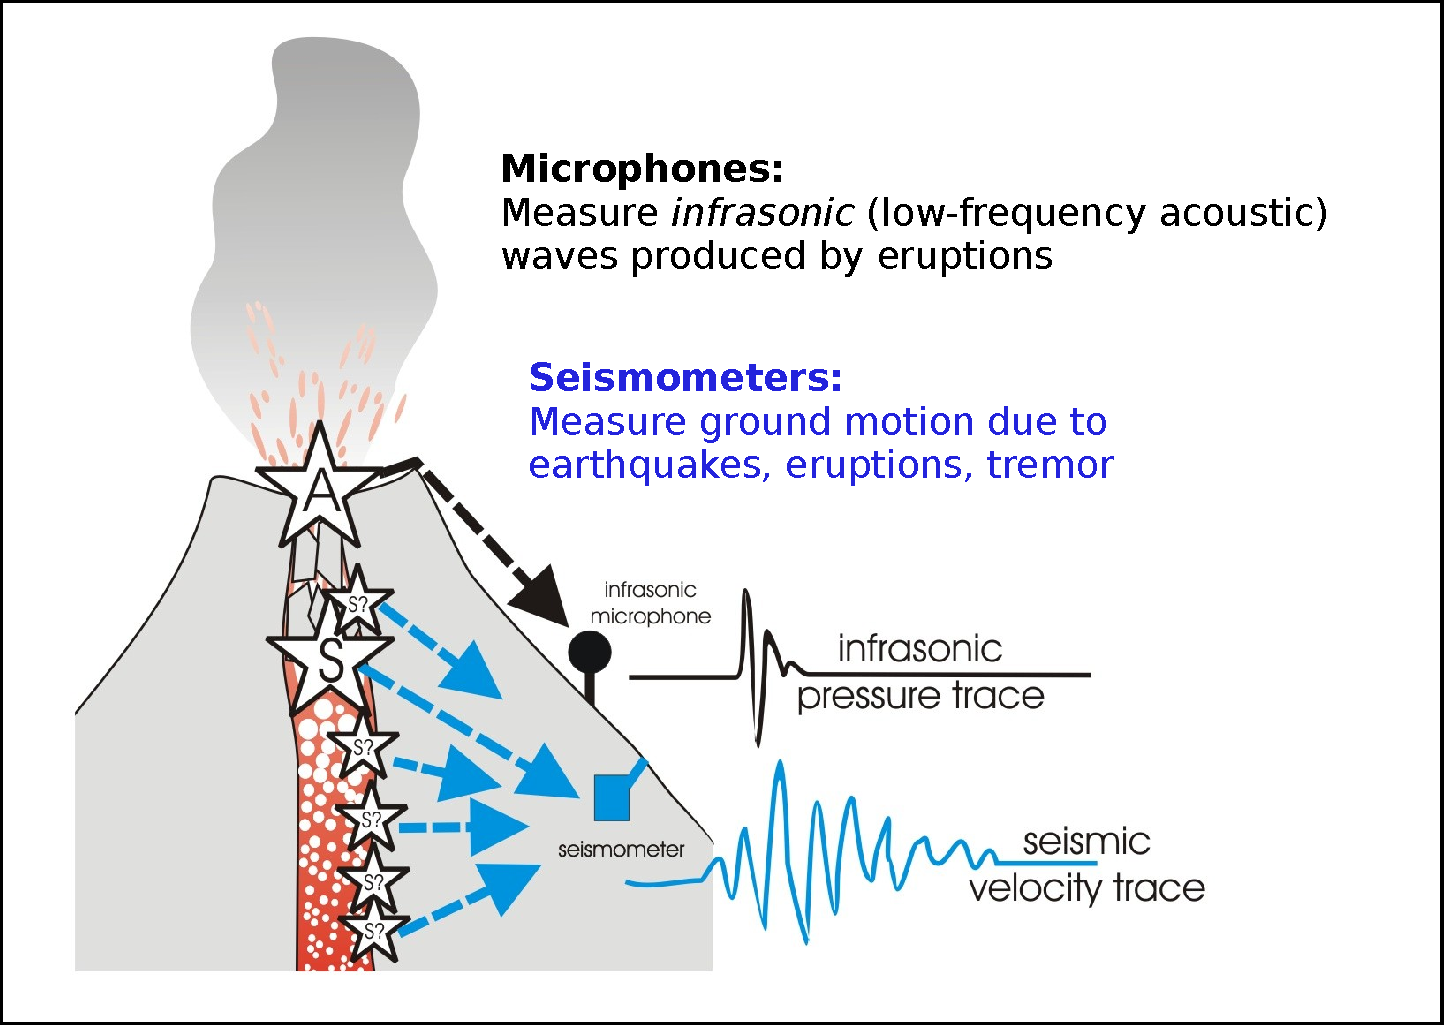
\includegraphics[width=0.9\hsize]{./2-related/figs/NewCartoon.pdf}
\end{center}
\caption{\textbf{Sensors used for volcano monitoring.}}
\label{introduction-fig-cartoon}
\end{figure}

The geophysics community has well-established tools and techniques used to
process the signals extracted by volcanic data collection networks. These
analytical methods require that our wireless sensor network provide data of
extremely high fidelity. A single missed or corrupted sample can invalidate
an entire portion of data. Small differences in sampling rates between two
nodes can frustrate analysis. Samples must be accurately time-stamped to
allow comparisons between nodes and between networks.

An important feature of volcanic signals is that much of the data analysis
focuses on discrete events, such as eruptions, earthquakes, or tremor
activity. Although volcanoes differ significantly in the nature of their
activity, during our deployment many of the interesting signals at Reventador
spanned fewer than 60~s and occurred at the rate of several dozen per day.
This allowed us to design the network to capture time-limited events, rather
than continuous signals.

This is not to say that recording individual events is adequate to answer all
of the scientific questions volcanologists pose. Indeed, understanding
long-term trends requires complete waveforms spanning long time intervals.
However, the low radio bandwidth of typical wireless sensor nodes makes them
inappropriate for these types of studies and for this reason we have focused
on triggered event collection.

\subsection{Existing Volcano Instrumentation}

\begin{figure}[t]
\begin{center}
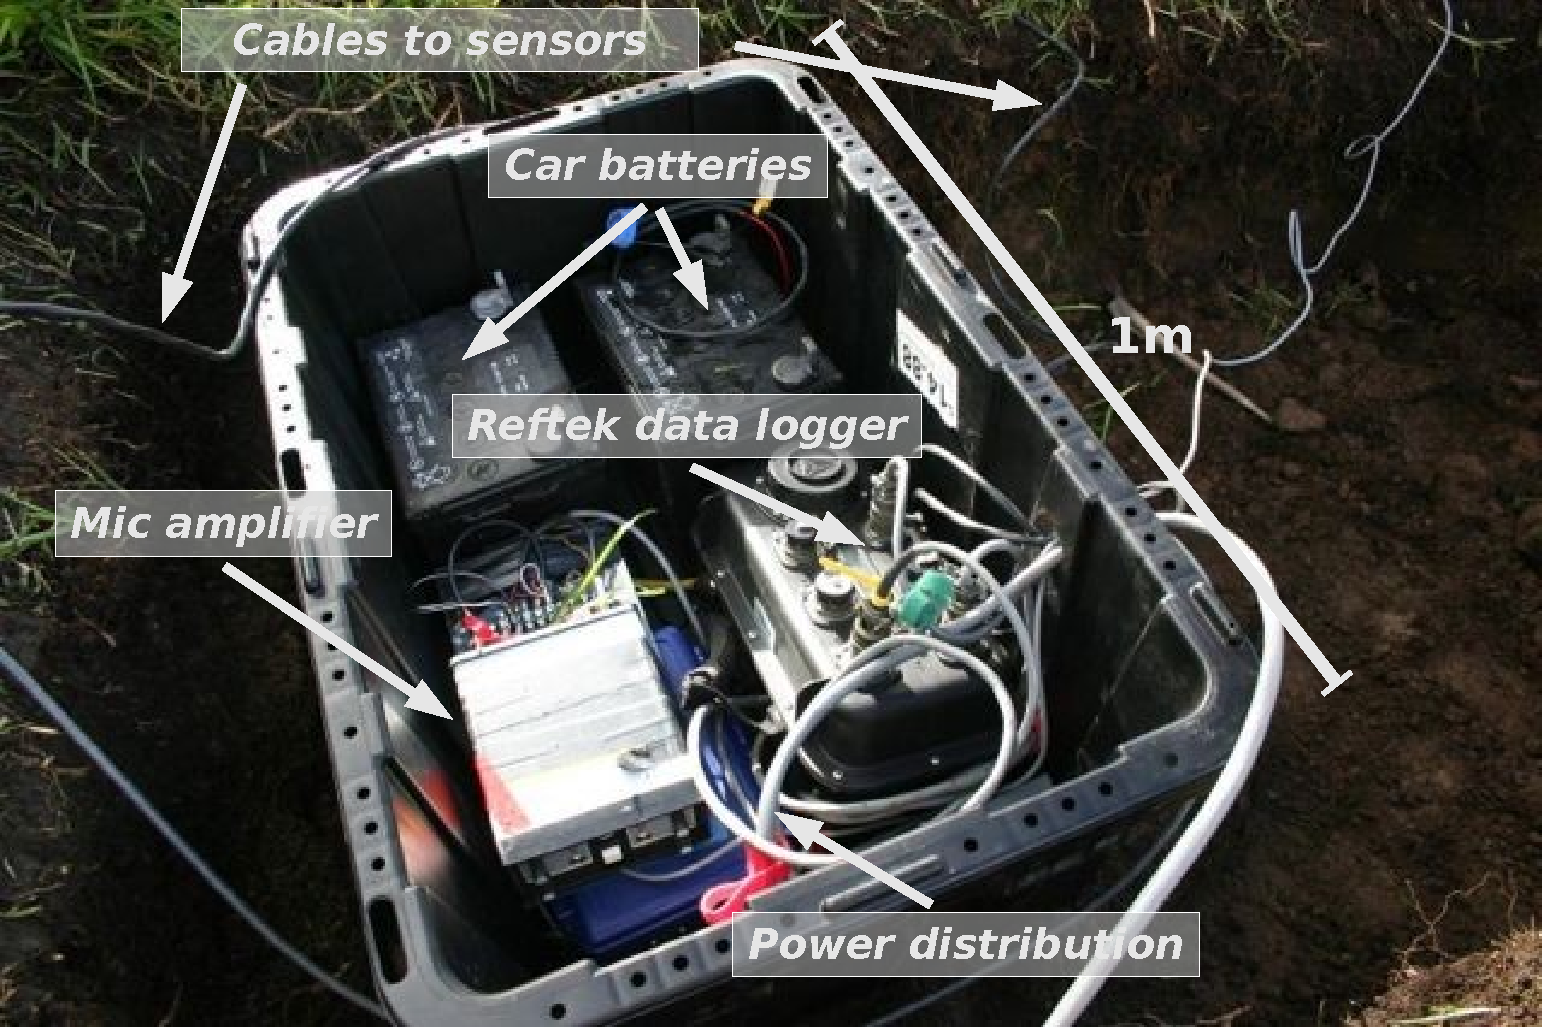
\includegraphics[width=0.9\hsize]{./2-related/figs/Standalone.pdf}
\end{center}
\caption{\textbf{Wired seismoacoustic monitoring station.}}
\label{related-fig-standalone}
\end{figure}

The type of instrumentation used to study volcanoes depends on the the
science goals of the deployment. Geophysicists often use standalone
dataloggers (e.g., Reftek 130-01~\cite{reftek}) that record signals from
seismometers and microphones to a flash drive. These data loggers are
expensize (\~\$9,000) bulky (8500~$cm^2$), heavy (2~kg) and power-hungry
(1~to~2.1W), typically powered by lead-acid car batteries (14.5~kg each)
charged by large (1~$m^2$) solar panels. The sheer size and weight of the
resulting set of equipment precludes deployments of more than a small number
of stations in remote or hazardous areas.

Figure~\ref{related-fig-standalone} shows an example deployed wired
monitoring station with the components labeled. Such a setup would support
several high-resolution powered seismometers, acoustic microphones, and other
instruments. The power supply (two lead-acid car batteries), Reftek data
logger with Flash drive to store collected data, signal amplification and
power distribution components are stored together in a large container and
buried underground. The sensors --- in this case, powered seismometers and
microphones --- are deployed nearby with wired connections to the Reftek data
logger. A solar panel may also be located nearby to recharge the car
batteries and enable long-term operation.

Additionally, data must be retrieved manually from each station every few
weeks, involving significant effort. Analog or digital radio telemetry can
enable real-time transmission of data back to an observatory, and is
typically installed for monitoring stations intended to be permanent.
However, existing telemetry equipment is bulky and difficult to install, and
its limited radio bandwidth can preclude collecting large amounts of data
from multiple channels.

As a result, many short-duration scientific experiments use a stand-alone
data acquisition system at each recording station. The digitizer performs
high-resolution analog-to-digital conversion from the wired sensors and
stores data on a hard drive or Compact Flash card. However, these systems
require data to be manually retrieved from the station prior to processing,
which can be difficult or time-consuming depending on the location of the
station and the duration of the intended deployment. Depending on the size of
the recording media, a station may record several days or weeks worth of data
before it must be serviced.

\section{Opportunities for Wireless Sensor Networks}

\begin{figure}[t]
\begin{center}
\begin{tabular}{ccc}
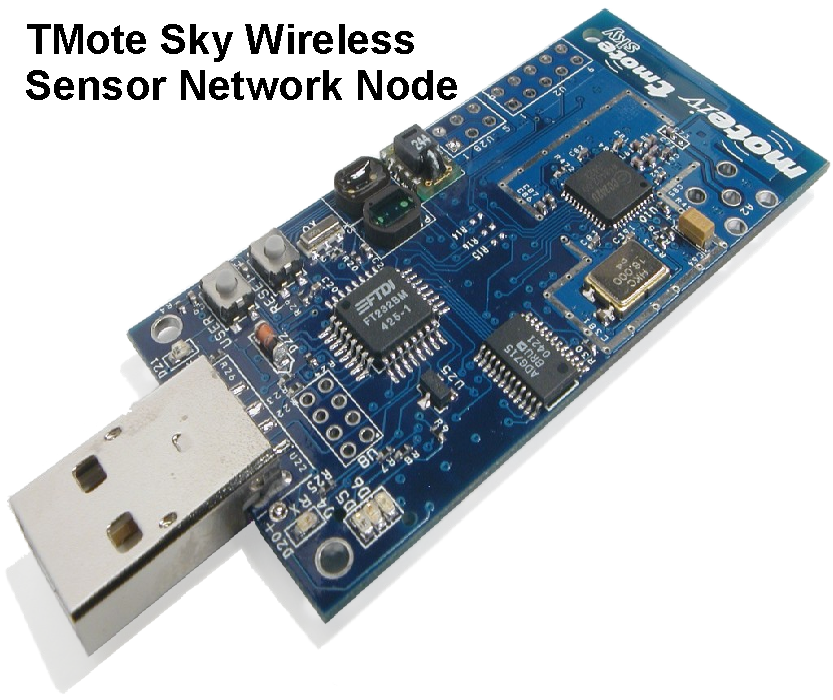
\includegraphics[width=0.3\hsize]{./2-related/figs/TMoteSky.pdf} &
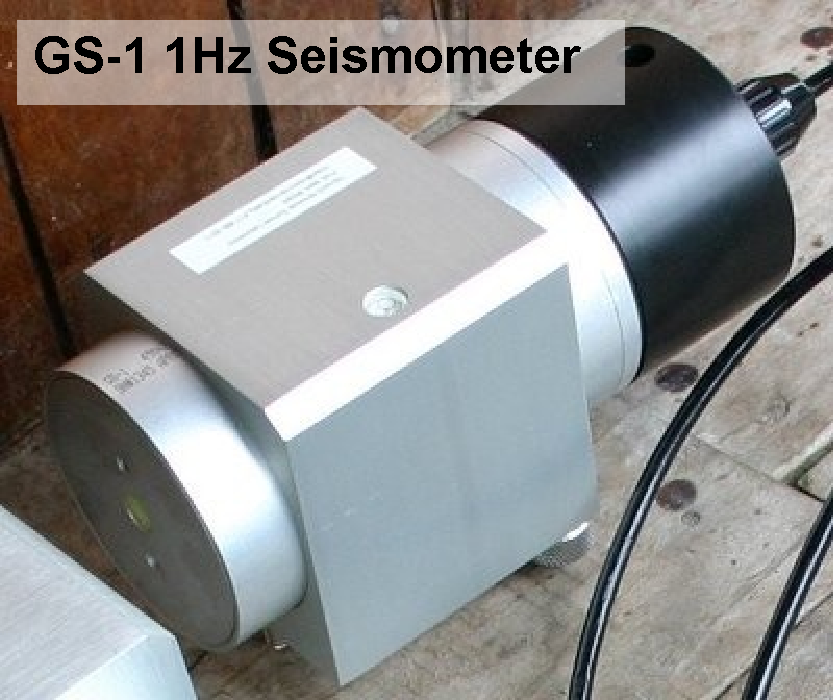
\includegraphics[width=0.3\hsize]{./2-related/figs/GS1.pdf} &
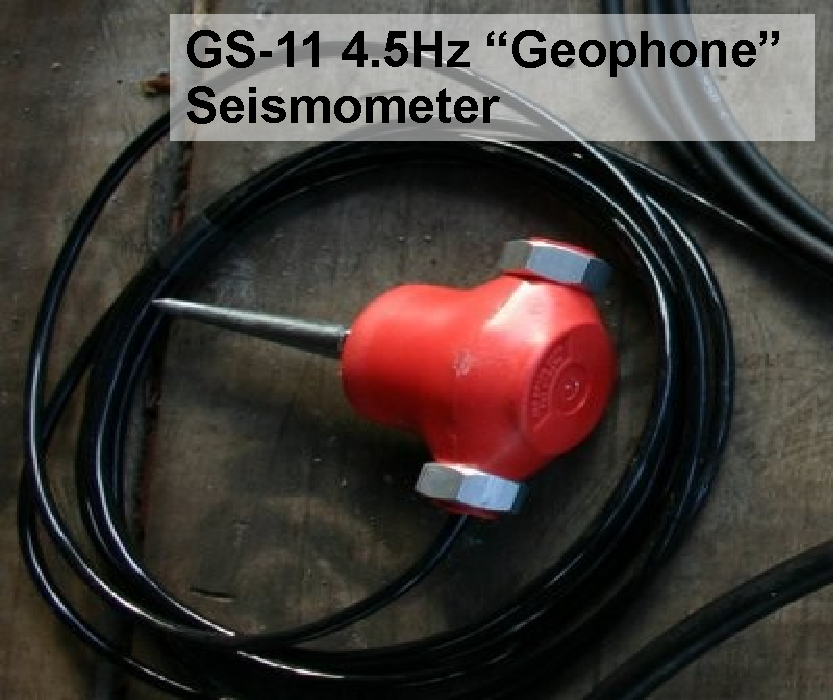
\includegraphics[width=0.3\hsize]{./2-related/figs/GS11.pdf} \\
\textbf{(a)} & \textbf{(b)} & \textbf{(c)} \\
\end{tabular}
\end{center}

\caption{\textbf{Equipment used by our volcano-monitoring sensor network.}
From left to right: (a) a TMote Sky sensor ``mote''; (b) a GS-1 1Hz
seismometer; (c) a GS-11 4.5Hz seismometer, or ``Geophone''. Both
seismometers are passive, single-axis instruments. The GS-1 is significantly
more expensive and accurate. Our deployment used primarily GS-11's, due to
their lower cost.}

\label{introduction-fig-equipment}
\end{figure}

Networks of spatially-distributed sensors are commonly used to monitor
volcanic activity, both for hazard monitoring and scientific
research~\cite{Scarpa96}. Typical types of sensing instruments include
seismic (see Figure~\ref{introduction-fig-equipment}~(b) and (c)), acoustic,
GPS, tilt-meter, optical thermal, and gas flux. Volcanic sensors range from
widely dispersed instrument networks to more confined sensor arrays. An
individual sensor station could consist of a single sensor (e.g., seismometer
or tilt sensor), or an array of several closely-spaced ($10^2$ to $10^3$~m
aperture) wired sensors, perhaps of different types. Multiple stations may be
integrated into a larger network installed over an extended azimuthal
distribution and radial distance ($10^2$ to $10^4$~m) from the volcanic vent.
Data from various stations may be either recorded continuously or as
triggered events and the acquisition bandwidth depends upon the specific data
stream. For instance, seismic data is often acquired at 24-bit resolution at
100~Hz, while tilt data may be recorded with 12-bit resolution at 1~Hz or
less.

Unfortunately, the number of deployed sensors at a given volcano is usually
limited by a variety of factors, including: monetary expenses such as sensor,
communication, and power costs; logistical concerns related to time and
access issues; and archival and telemetry bandwidth constraints. Due to their
small size (12.8~$cm^2$), light weight (0.015~kg without battery), low power
consumption (\~60~mW) and relatively low cost (\$79), wireless sensor nodes
such as the TMote Sky (see Figure~\ref{introduction-fig-equipment}~(a)) have
an important role to play in augmenting and extending existing seismic
instrumentation, providing the increased spatial resolution necessary to
support seismic applications like tomography.

\subsection{Challenges for Sensor Networks}

Wireless sensor networks have the potential to greatly enhance understanding
of volcanic processes by permitting large deployments of sensors in remote
areas. The science requirements give rise to a number of unique challenges
for sensor networks, which we outline below.

\begin{itemize}

\item \textbf{High-resolution signal collection.} Data from seismometers and
microphones must be recorded at relatively high data rates with adequate
per-sample resolution. A sampling rate of 100~Hz and resolution of 24~bits is
typical. This is in contrast to sensor networks targeting low-rate data
collection, such as environmental
monitoring~\cite{gdi-sensys04,berkeley-redwoods}.

\item \textbf{Triggered data acquisition.} Due to limited radio bandwidth
(less than 100~Kbps when accounting for MAC overhead), it is infeasible to
continuously transmit the full-resolution signal. Instead, we rely on
triggered data collection that downloads data from each sensor following a
significant earthquake or eruption. This requires sensor nodes to
continuously sample data and detect events of interest. Event reports from
multiple nodes must be collated to accurately detect \textit{global} triggers
across the network.

\item \textbf{Timing accuracy.} To facilitate comparisons of signals across
nodes, signals must be timestamped with an accuracy of one sample time (i.e.,
10~ms at 100~Hz). Data loggers generally incorporate a GPS receiver and use
low-drift oscillators to maintain accurate timing. However, equipping each
sensor node with a GPS receiver would greatly increase power consumption and
cost. Instead, we rely on a network time synchronization
protocol~\cite{rbs,ftsp} and a \textit{single} GPS receiver. However,
correcting for errors in the time synchronization protocol requires extensive
post-processing of the raw timestamps.

\end{itemize}

\section{Related Work}
\label{sec-relatedwork}

This section discusses four kinds of related systems, those designed to cope
with high data rates, designed to operate in scientific contexts, and related
to Lance or IDEA.

\subsection{High Data Rate Sensing}

Many sensor network applications require collecting high-resolution signals
using low-power nodes. Examples include monitoring acoustic, seismic, and
vibration waveforms in bridges, industrial equipment, and animal habitats.
These systems all attempt to acquire high data rate (100~Hz or higher),
high-fidelity data across the network subject to severe constraints on radio
bandwidth and energy usage.

A group from UC Berkeley performed the largest deployment to date of sensor
network nodes for structural health monitoring: 46 nodes placed on the Golden
Gate Bridge~\cite{ggb-ipsn07}. Nodes collect vibration data at 1~kHz, and the
network uses many of the same routing and time synchronization protocols used
by our volcano monitoring system. A special bulk data collection protocol,
called Straw, was developed for the deployment. The highly linear topology of
the deployed network was later used to test the Flush data collection
protocol~\cite{flush-sensys07}. The deployment at the Golden Gate Bridge also
gave rise to a system called the Structural Health Monitoring Toolkit
(Sentri) that interfaces between the outside world and the sensor network by
transmitting commands to nodes as necessary.

NetSHMis a wireless sensor network for structural health monitoring, which
involves studying the response of buildings, bridges, and other structures to
localize structural damage, e.g., following an
earthquake~\cite{netshm-ewsnsubmission,netshm-emnets05,wisan}. This system
shares many of the challenges of geophysical monitoring. Indeed, the data
rates involved (500~Hz per channel) are higher than are typically used in
volcano studies. The Wireless Modular Monitoring System (WiMMS) is another
structural monitoring network with similar goals that has been validated both
in field deployments at the Geumdang Bridge in Icheon, South Korea, and in
laboratory tests~\cite{wimms-lynch06}. This system is designed to supporting
decentralize control algorithm that respond to structural changes using
actuators. In this context decentralization reduces the amount of data that
must be transmitted to a central location while eliminating the base station
as a single point of failure.

NetSHM implements reliable data collection using both hop-by-hop caching and
end-to-end retransmissions. The work explores the use of local computations
on sensors to reduce bandwidth requirements. Rather than a global
time synchronization protocol, the base station timestamps each sample upon
reception. The \textit{residence time} of each sample as it flows from sensor
to base is calculated based on measurements at each transmission hop and used
to deduce the original sample time.

Several factors distinguish our work on volcano science from structural
monitoring applications. First, structural monitoring networks typically
either collect data following controlled excitations of a structure or at
periodic intervals, which simplifies transmission scheduling. In our case,
volcanic activity is bursty and highly variable, requiring more sophisticated
approaches to event detection and data transfer. While the Golden Gate Bridge
system is sparsely deployed like our volcano sensor networks, many structural
monitoring applications are deployed in relatively dense networks, making
data collection and time synchronization more robust. 

Condition-based maintenance is another emerging area for wireless sensor
networks. The typical approach is to collect vibration waveforms from
equipment (e.g., chillers, pumps, etc.) and perform time- and
frequency-domain analysis to determine when the equipment requires servicing.
Intel Research has explored this area through deployments at a fabrication
plant and an oil tanker in the North Sea~\cite{intel-northseasensys}.
Although this application involves high sampling rates, it does not
necessarily require time synchronization as signals from multiple sensors
need not be correlated. The initial evaluation of these deployments only
considers the network performance and does not address data fidelity issues.

While many early environmental monitoring applications are characterized by
low data rates, some have focused on applications requiring high-speed data
acquisition. An example application is monitoring colonies of marmots. A
group at MIT led by Lew Girod has explored several generations of hardware
and software solutions for distributed acoustic monitoring driven by this
application~\cite{girod-marmots}. This work produced the Acoustic
ENSBox~\cite{girod-ensbox}, a self-calibrating hardware solution designed to
be easy to deploy in support of acoustic sensing applications. The ENSBox
features an ARM processor, which puts it at a different point on the
power-performance curve from typical sensor network nodes and makes it more
suitable for the high-speed processing necessary to capture acoustic signals.

The software environment for the ENSBox was originally provided by
EmStar~\cite{emstar}, which targets Linux-based platforms. More recently, the
ENSBox has been used as the basis of the VoxNet platform, an environment
designed for acoustic signal collection and processing.
VoxNet~\cite{voxnet-ipsn08} is comprised of three pieces:
Wavescope~\cite{wavescope}, a programming environment targeting
heterogeneous sensor networks. Wavescope programs are written in
WaveScript~\cite{wavescript-techreport08}, a stream-processing language.
Users compose a set of filters and other stream operators into a ``script''
similar to a data-flow graph.

The VoxNet platform includes a variety of network services, such as
time synchronization, routing, and node localization that applications
running in this environment can make use of. Once the program is written and
installed on nodes, VoxNet includes a set of control and visualization tools
intended to allow users to interact with the running system and view the data
as it is collected. A system using VoxNet was deployed in 2008 at the Rocky
Mountain Biological Laboratory and used to study the alarm calls of marmots.
Acoustic monitoring has scientific applications to other species as well, as
a variety of animals and birds produce scientifically-interesting
vocalizations.

Another application of high data rate sensing to habitat monitoring is the
cane toad monitoring project run by a team at Portland State University,
CSIRO, and the University of New South Wales. The cane toad is an invasive
species in Australia, and their spread is being monitored due to concerns
about their impact on the country's native fauna. The goals of the project
are to design a system permitting \textit{in situ} classification of various
frog species based on their vocalizations.

After completing a pilot study, two additional iterations advanced the design
of the system. In the first, a hybrid network was developed, mating low-power
sensor nodes and middle-tier devices with more advanced processing and
storage capabilities. Data reduction is performed on the sensor nodes in
order to limit the amount of information that must be sent to the high-power
devices, thus prolonging the lifetime of the embedded
nodes~\cite{canetoad-tosn}. The second iteration explores compressive
sampling techniques and also deploys a classification algorithm that can be
run directly on the resource-constrained sensor nodes.

Camera-based sensor networks also produce high data rates and have been the
subject of considerable study. A group at UCLA built a system called
Cyclops~\cite{cyclops-sensys05} which brings vision technology to sensor
network devices by offering a low-power imaging devices better suited to mating
with resource-constrained sensor nodes. They show that Cyclops nodes can
successfully perform fundamental vision-recognition tasks such as object
detection and hand posture recognition. Another team at UMass Amherst sees
motes fitted with imagers as forming one tier of a multi-tier multi-modal
($M^2$) sensor network~\cite{m2-nossdav05}. Such $M^2$ networks consist of
several tiers operating at different power levels while attempting to combine
the capabilities of multiple types of devices. The lowest tier might consist of
low-power sensor nodes equipped with vibration sensors and be used to trigger
the operation of more power-hungry devices --- such as
Stargates~\cite{stargate} fitted with webcams --- in the upper tiers.

\subsection{Scientific Sensing}

The first generation of sensor network deployments focused on distributed
monitoring of environmental conditions. Representative projects include the
Great Duck Island~\cite{spm:04habitat,polastre-masters,mainwaring-habitat},
Berkeley Redwood Forest~\cite{berkeley-redwoods}, and James
Reserve~\cite{cerpa-habitat} deployments. These systems are characterized by
low data rates (sampling intervals on the order of minutes) and very
low-duty-cycle operation to conserve power. Research in this area has made
valuable contributions in establishing sensor networks as a viable platform
for scientific monitoring and developing essential components used in our
work. 

This previous work has not yet focused on the efficacy of a sensor network as
a scientific instrument. The best example is the Berkeley Redwood Forest
deployment~\cite{berkeley-redwoods}, which involved 33~nodes monitoring the
microclimate of a redwood tree for 44~days. Their study focuses on novel ways
of visualizing and presenting the data captured by the sensor network, as
well as on the data yield of the system. The authors show that the
microclimactic measurements are consistent with existing models, but ground
truth of the data is not established. This paper does highlight many of the
challenges involved in using wireless sensors to augment or replace existing
scientific instrumentation.

A group at UCLA has built a system for soil monitoring and deployed it in the
AMARSS transect in the James Reserve, a biological field station operated by
the University of California. The goal was to augment a set of wired data
loggers with wireless sensor technology, similar in spirit to what we have
attempted with our volcano monitoring system. Since 2005 the deployed system
has collected over 26~million measurements, which are retrieved periodically
by a technician visiting the deployment site. The goal is to study the carbon
cycle and estimate the flux of carbon dioxide from the soil.

The largest challenge facing these researchers was coping with missing data.
To address it, they built a system called Suelo~\cite{suelo-sensys09}.  Suelo
is intended to aid human researchers in monitoring and assisting the health
of the deployment, sense the soil-monitoring sensors used are quite fragile.
Suelo monitors the readings capture by the network and tries to distinguish
between ``interesting'' and ``faulty'' data, and initiating human
intervention when sensors require replacement or recalibration.

Computer scientists at UMass Amherst have been deploying GPS-enabled sensors
to study the movement of a threatened species of turtle. This work led to
Eon, a language and runtime system designed to enable energy-aware
programming. Eon claims to be the first energy-aware programming language and
tries to make resource usage explicit to programmers by allowing them to
annotate their code with energy states. At runtime, Eon will adapt the
behavior of the node based on resource availability.

Similar to our work in its application to environmental hazard mitigation,
previous projects have explored sensor networks for flood and landslide
detection, at MIT and John Hopkins University, respectively. The MIT system
feeds data from a network of sensors into a model designed to predict
rainfall-triggered flooding~\cite{basha-sensys08}. They were able to show the
demonstrate the accuracy of their approach using data collected over multiple
field deployments on Honduras between 2004 and 2007. JHU's approach to
landslide detection employs sensor columns, vertical underground
installations of several different sensors~\cite{landslide-sensys05}. When a
portion of the deployed network detects that a slip surface is forming, nodes
cooperate to estimate the position of the slip surface which is fed into a
model that predicts whether and when a landslide will occur. Both of these
projects differ from our work by involving significant modeling and
prediction components, whereas we have focused primarily on raw data
collection.

Of particular interest is ongoing work at Washington State University using
camera-dropped sensor networks to monitor the activity of Mt. St.
Helens~\cite{wsuvolcano-mobisys09}. This project shares many of our goals,
including ease of deployment and data fidelity, but differs in its focus on
system lifetimes of up to 1~year, and in its aim to replace, rather than
augment, existing volcano monitoring stations. The reliance on helicopter
support while deploying nodes also leads to a different set of design
decisions, including much larger batteries and more capable nodes.

The WSU group uses an iMote2~\cite{imote2} sensor node, which shares the
CC2420 802.15.4 radio with our TMote but features the PXA271 XScale processor
with significantly more computational horsepower than the MSP430. The
expanded form factor and power budget permits the use of GPS at each node,
simplifying time sychronization (although FTSP is available as a backup if
the GPS signal is lost).

While the system aims to provide continuous data collection, the limited
bandwidth of the 802.15.4 radios on each sensor node and the 900~MHz
Freewave~\cite{freewave} modem used to maintain a connection with the
observatory limit the data that can be collected. Similar to our
volcano-monitoring system, an impulse detector implemented as a short-term
average over long-term average (STA/LTA) is used to assign a priority to the
data as it is collected. Data prioritization is used during data collection
and routing to ensure that data from detected events reaches the observatory
first. Currently the system works around energy limitations by using heavy
AIR-ALKALINE batteries, which are feasible because the nodes are being
deployed by helicopter.

\subsection{Data Quality Optimization Frameworks}
\label{lance-sec-related}

Several systems are related to Lance but differ substantially in their goals
and assumptions.

EnviroMic~\cite{enviromic} is a system designed to support distributed
acoustic recording by leveraging the collective storage resources of multiple
sensor nodes. It performs cooperative recording by organizing nodes into
groups when multiple nodes detect the same acoustic event, and using these
groups to ensure that only one node is recording acoustic data for as long as
the event of interest continues. This is intended to reduce the amount of
data that must be stored by eliminating redundant signal collection.

EnviroMic also focuses on distributing the storage load within the network to
ensure that the distributed storage can be utilized and signals of interest
not lost due to full Flash drives. While nodes may exchange data to rebalance
storage during the experiment, the fundamental assumption of the architecture
is that data will be manually retrieved from sensor nodes following the
deployment. Unlike Lance, EnviroMic is not intended for applications with
real-time data needs.

ICEDB~\cite{zhang2007icedb} supplies a delay-tolerant and priority-driven
query processor for the CarTel~\cite{cartel} system. ICEDB provides SQL
extensions allowing queries to assign both inter- and intra-stream
priorities, which are used by the query processor to manage bandwidth and
storage resources. ICEDB also uses a similar node-level summarization
technique to that used by Lance.

While ICEDB considers bandwidth limitations, it does not consider energy as a
constraint. The fundamental goal of ICEDB --- to provide database-like access
to mobile nodes that may experience periods of disconnection or poor
connectivity --- differs from that of Lance, which explains the architectural
differences. CarTel nodes are much higher-power and assumed to be attached to
power sources in the vehicles that they are deployed in.

VanGo~\cite{vango} provides an architecture for collecting and processing
high-resolution sensor data on resource-constrained nodes. VanGo focuses on a
programming model based on a linear filter chain and implementing efficient
signal-processing operations with limited computational power.
WaveScope~\cite{wavescope} and Flask~\cite{flask-tr} are languages for stream
processing applications. These systems are largely complementary to Lance,
and could be used to process signal data prior to collection, although our
focus is on collecting \textit{raw} sensor data from large networks. These
systems do not attempt to optimize data collection under varying energy and
bandwidth constraints. 

\subsection{Energy Load-Balancing Services}
\label{idea-sec-related}

Previous work has addressed the problem of energy load balancing in contexts
such as sensor coverage, role assignment, and energy-aware routing. Other
efforts in sensor networks have focused on reducing the power consumption at
individual nodes without considering energy distribution. Many of these
efforts are specific to a particular application or component and do not
provide a service like IDEA that can be used by a variety of applications. 

A number of existing systems such as Odyssey~\cite{odyssey-osr99},
PowerScope~\cite{powerscope-wmcsa99} and more recently
Cinder~\cite{cinder-mobiheld09}, have addressed measuring or adapting to
energy variations on battery-powered devices, primarily to support mobile
applications. This naturally produces a difference in approach from IDEA,
since IDEA targets networks consisting of multiple nodes but treated as a
single entity. Since nodes are collaborating we can enable more sharing and
ask nodes to sacrifice for each other, whereas mobile device users would
likely be upset if they discovered that their phone was running low on power
because it was trying to improve the lifetime of a stranger's phone located
nearby.

Quanto~\cite{quanto-osdi08} provides a framework for tracking and
understanding energy consumption in embedded sensor systems. The existence of
systems such as Quanto was a primary motivation for IDEA, since the
visibility distributed resource tracking provides creates an opportunity to
adapt to changes in availability across the network. Currently IDEA requires
that components model their own energy consumption, which may be difficult
for components with complex behavior. We are exploring integrating Quanto
into IDEA to provide more precise tracking of energy at runtime, which could
eliminate the need for component-specific modeling and ease the process of
integrating applications with IDEA.

Eon~\cite{eon-sensys07} performs similar energy tracking and forward
projection but focuses on single-node, not network-wide adaptations.
SORA~\cite{sora-nsdi05} focuses on decentralized resource allocation based on
an economic model in which nodes respond to incentives to produce data or
perform specific tasks, with each node trying to maximize its profit for
taking a series of actions. While SORA, using correctly set prices, could
produce similar network-wide behavior to that enabled by IDEA, the connection
between prices and the behavior of the network is not completely clear. IDEA
simplifies the problem of global network control through the energy objective
function which encapsulates the application's goal.

Some work on energy-aware routing~\cite{ShahRabaey2002,381685} has addressed
equitable energy distribution within the network by probabilistically
choosing between multiple good paths between each source and sink pair.
LEACH~\cite{leach} and other similar approaches attempt to distributed energy
in an entirely decentralized way, using local heuristics to do so.
Lexicographically maximum rate allocation~\cite{fairrate-sensys08} uses a
decentralized algorithm to tune optimum data collection rates in perpetual
networks when static routes are used, all nodes route to a single sink, and
the recharging profiles of the nodes are known ahead of time. Rate allocation
could be implemented in IDEA and comparing the two is planned future work.

VigilNet~\cite{vigilnet} is a target-tracking system that attempts to save
energy by rotating ``sentry'' duties between a group of nearby nodes. Nodes
that are not assigned as sentries can sleep and conserve energy while the
sentry monitors the area. When an event occurs, the sentry awakes nearby
nodes and initiates the tracking process. VigilNet assigns sentry duties
based on each node's energy availability while trying to ensure that the
entire area being monitoring is covered. Given the desire both to extend
system lifetime and maintain a desired application fidelity, VigilNet could
be implemented using IDEA, allowing both energy availability and harvesting
to be considered when assigning setries.

EnviroMic~\cite{enviromic} is a distributed acoustic storage system for
sensor networks. When EnviroMic nodes hear an acoustic event, a leader is
elected to assign recording tasks to nodes in the group. As storage space is
limited, EnviroMic attempts to push data to quiet sections of the network
with unused storage, balancing storage consumption across the network. Both
of these tasks involve choosing from a set of nodes that can perform the same
storage task, and so EnviroMic could be integrated with IDEA allowing the
energy overheads of data transfers to be considered.

The IDEA architecture emerged from our own prior work on energy management
for wireless sensor networks, including Lance (Chapter~\ref{chapter-lance})
Pixie~\cite{pixie-sensys08}, and Peloton~\cite{peloton-hotos09}. Pixie
proposed an operating system and programming framework for sensor network
nodes that promotes resources to a first-class primitive, using tickets to
manage resource consumption and brokers to enable specialized management
policies. Pixie does not consider the energy impact of a node on other nodes.

Peloton proposed an architecture for distributed resource management in
sensor networks combining state sharing, vector tickets to represent
distributed resource consumption and a decentralized architecture in which
nodes serve as ticket agents managing the resource consumption of themselves
and on behalf of nearby nodes. IDEA shares many features with Peloton and can
be viewed as the beginnings of an implementation of the Peloton design, with
state sharing to enable energy decision making and every node serving as a
ticket agent for itself but considering the distributed impact of its own
local state.


\chapter{Evaluation of 2005 Deployment}
\label{chapter-evaluation}

In this chapter, we take a hard look at the performance of a wireless sensor
network deployed on an active volcano. We evaluate its effectiveness as a
scientific instrument using two metrics: data \textit{fidelity} and
\textit{yield}. Fidelity encompasses the quality and consistency of retrieved
seismoacoustic signals, while yield reflects the quantity of data delivered
by the network. 

The core contribution of this chapter is an analysis of the efficacy and
accuracy of a volcano-monitoring sensor network as a scientific instrument.
In this chapter, we evaluate the data collected from a 19-day field
deployment of 16~wireless sensors on Reventador volcano, Ecuador, along the
following axes:

\begin{itemize}

\item \textbf{Robustness:} We find that the sensor nodes themselves were
extremely reliable but that overall robustness was limited by power outages
at the base station and a single three-day software failure. Discounting the
power outages and this single failure, mean node uptime exceeded 96\%.

\item \textbf{Event detection accuracy:} Our network was designed to trigger
data collection following volcanic events such as earthquakes and eruptions.
We measure the accuracy of our distributed event-detection algorithm, finding
that the algorithm has a zero false positive rate. However, the network
failed to detect many seismic events due to a poor choice of event-detection
parameters and limitations of our data collection protocol.

\item \textbf{Data transfer performance:} We evaluate the ability of our data
collection protocol to transfer complete signals following an event. We find
a 90th percentile \textit{event yield} (fraction of nodes for which all data
for an event was collected) of 94\% and a latency of 63~sec per radio hop for
downloading 60~sec worth of data.

\item \textbf{Timing accuracy:} Data collected by each node must be
timestamped to within a single sample time (10~ms) to enable seismological
analysis. We evaluate the stability of the underlying time synchronization
protocol (FTSP~\cite{ftsp}), and develop a novel approach to \textit{time
rectification} that accurately timestamps each sample despite failures of the
FTSP protocol. We show that this approach recovers timing with a
90th-percentile error of 6.8~msec in a 6-hop network.

\item \textbf{Data fidelity:} Finally, we take a seismological view of the
captured data and present a head-to-head comparison of data recorded by our
sensor network against a colocated data logger. We also evaluate the
consistency of the recorded signals in terms of seismic and acoustic wave
arrival times across the network, showing that the data is consistent with
expected physical models of the volcano's activity.

\end{itemize}

\XXXnote{GWA: TODO: Rewrite this.}

The rest of this chapter is organized as follows.
Sections~\ref{evaluation-sec-robustness} through
\ref{evaluation-sec-fidelity} present a detailed analysis of the network's
performance along each of the evaluation metrics described above.
Section~\ref{evaluation-sec-lessons} presents several lessons learned from
the deployment.
 
\section{Overview of Three Deployments}

\begin{figure}[t]
\begin{center}
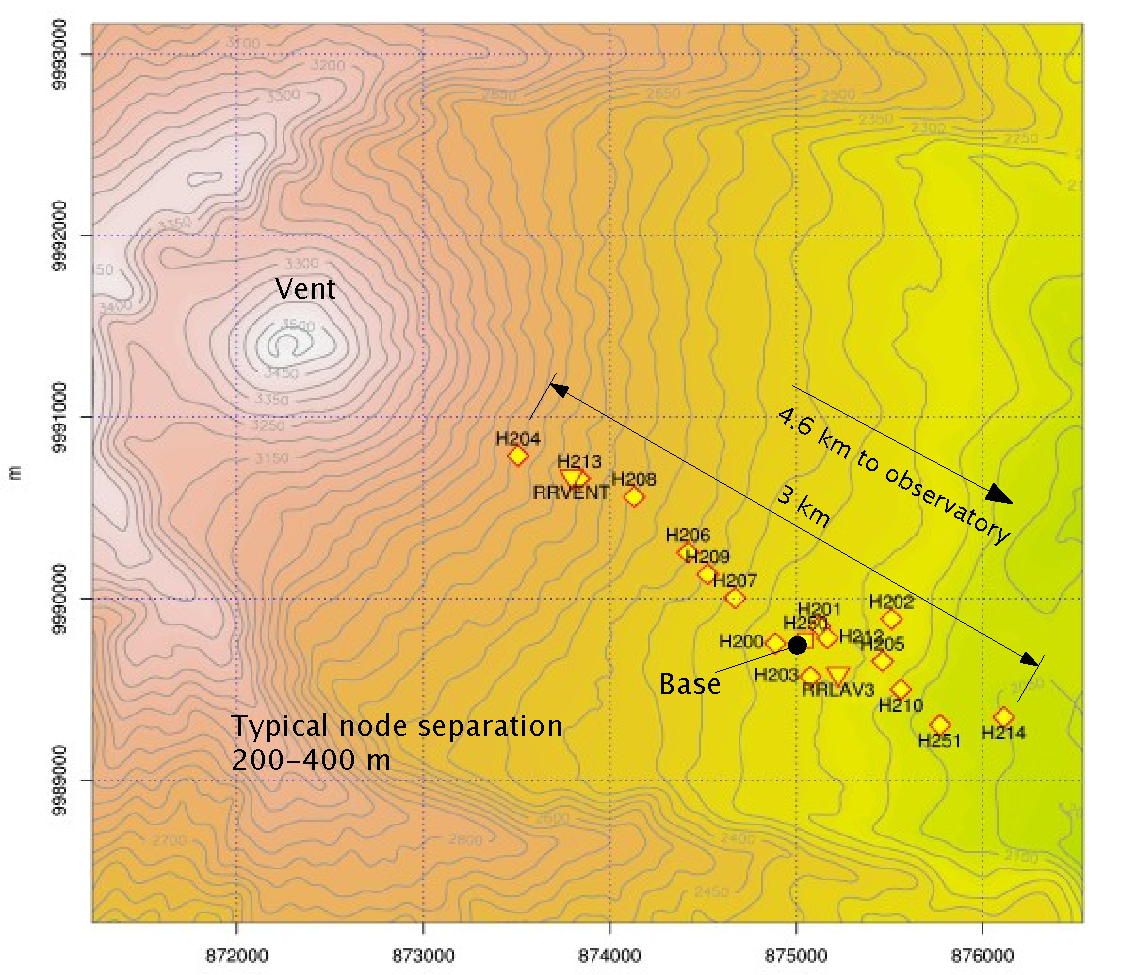
\includegraphics[width=0.8\hsize]{./5-evaluation/figs/2005-deployment-map.pdf}
\end{center}
\caption{\textbf{2005 deployment location.} The figure shows the location of
our second volcano deployment in 2005: 16 nodes deployed on Reventador
Volcano.}
\label{introduction-fig-deployment-map-2005}
\end{figure}

In total, we have performed three deployments of iterations of our system at
active volcanoes in Ecuador. Figs.~\ref{introduction-fig-deployment-map-2005}
and \ref{introduction-fig-deployment-map-2007} show the location and layout
of the second and third deployment. All three are summarized below:

\begin{figure}[t]
\begin{center}
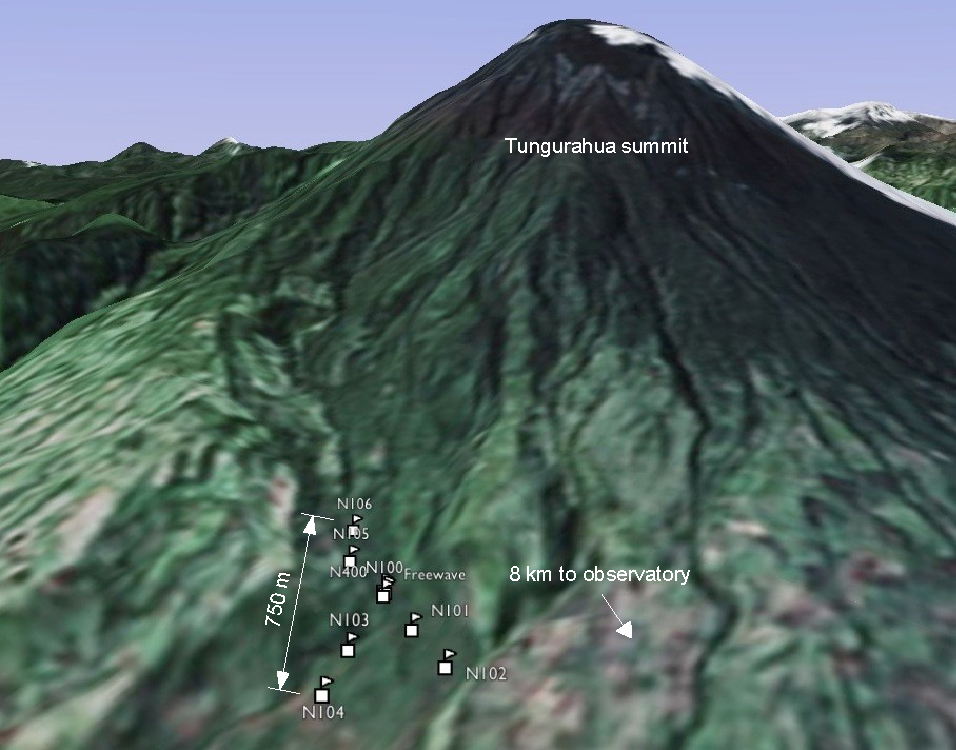
\includegraphics[width=0.8\hsize]{./5-evaluation/figs/2007-deployment-map.pdf}
\end{center}
\caption{\textbf{2007 deployment location.} The figure shows the locations of
our third volcano deployment in 2007: eight nodes deployed on Tungurahua
Volcano.}
\label{introduction-fig-deployment-map-2007}
\end{figure}

\begin{enumerate}

\item \textbf{July, 2004, Tungurahua Volcano:} We deployed three infrasonic
monitoring nodes continuously transmitting at 102~Hz to a central aggregator
node, which relayed the data over a wireless link to the observatory
approximately 9~km away.  Our network was active from July 20--22, 2004, and
collected over 54~hours of infrasonic signals.

\item \textbf{August, 2005, Reventador Volcano:} This deployment featured a larger,
more capable network consisting of sixteen nodes fitted with seismoacoustic
sensors deployed in a 3~km linear array.  Collected data was routed over a
multi-hop network and over a long-distance radio link to a logging laptop
located at the observatory 9~km away from deployment site.  Over three weeks
the network captured 230 volcanic events.

\item \textbf{July, 2007, Tungurahua Volcano:} We returned to Tungurahua Volcano in
2007 and deployed eight sensor nodes in order to test Lance, a framework for
optimizing high-resolution signal collection. The network was operational for
a total of 71~hours, during which time we downloaded 77~MB of raw data.

\end{enumerate}

\section{Deploying on Volc\'{a}n Reventador}

Volc\'{a}n Reventador is located in northern Ecuador, a three hour drive from
the capital, Quito.  Long dormant, Reventador reawakened suddenly in 2002,
erupting with massive force.  Ash thrown into the air blanketed the streets
of Quito 100~km to the east, closing schools and the airport.  Pyroclastic
flows raced down the mountain flattening forests, displacing an oil pipeline,
and severing a major highway.  After 18 months of quiescence, renewed
activity began in November 2004.  During our deployment, Reventador's
activity was characterized by discrete, relatively small explosive events,
ejecting incandescent blocks, gas, and ash several times a day.
Corresponding seismic activity was manifested by explosion earthquakes,
extended-duration shaking (tremor), and shallow rock fracturing earthquakes
that may have been associated with magma migration within the volcano.

Several features of Volc\'{a}n Reventador made it ideal for our
experiment.  Reaching 3,500~meters at its peak, Reventador sits at a
low elevation compared to other Ecuadorean volcanoes making deployment
less strenuous.  Its climate is moderate with temperatures ranging
between 10 and 30 degrees Celsius.  Pyroclastic flows produced by the
large explosion in 2002 left large parts of the flanks denuded of
vegetation.  With the effectiveness of our radio antennas severely
degraded by obstacles to line-of-sight, the lack of vegetation
simplified sensor node positioning.

Our base while working at Reventador was the Hosteria El Reventador, a small
hotel located nearby on the highway from Quito to Lago Agria.  The hotel
provided us with space to set up our equipment and ran an electric generator
to power our laptops and other equipment at the makeshift observatory.

\subsection{Network Hardware}

Our network consisted of 16~stations equipped with seismic and acoustic
sensors.  Each station consisted of a Moteiv TMote Sky~\cite{moteiv} wireless
sensor network node, an 8~dBi~2.4GHz external omnidirectional antenna,
seismometer, microphone, and a custom hardware interface board.
Fourteen~nodes were fitted with a Geospace Industrial GS-11 geophone, a
single-axis seismometer with a corner frequency of 4.5~Hz, oriented in the
vertical plane of motion.  The remaining two~nodes were equipped with
triaxial Geospace Industries GS-1 seismometers with corner frequencies of
1~Hz, yielding separate signals in each of the three axes.

The TMote Sky is a descendant of the UC Berkeley Mica ``mote'' sensor node.
It features a Texas Instruments MSP430 microcontroller, 48~KB of program
memory, 10~KB of SRAM, 1~MByte of external flash memory and a 2.4GHz Chipcon
CC2420 IEEE 802.11.4 radio.  The TMote Sky was designed to run
TinyOS~\cite{tinyos-asplos00}, and all of our software development made use
of this environment.  We chose the TMote Sky for several reasons.  The MSP430
microprocessor provides a large number of configurable ports, easily
supporting external devices.  The large amount of flash memory was useful for
buffering collected data, as described below.

We built a custom hardware board to integrate the TMote Sky with the
seismoacoustic sensors.  The board features up to four Texas Instruments
AD7710 analog to digital converters (ADCs) providing up to 24~bits per
channel of resolution.  Although the MSP430 microcontroller provides on-board
ADCs, they are unsuitable for our application.  First, they provide only
16~bits of resolution while we required at least 20~bits.  Second,
seismoacoustic signals require an aggressive filter centered around 50~Hz.
Due to the infeasibility of implementing such a filter using analog
components, it is usually approximated digitally, requiring several factors
of oversampling.  To perform this filtering, the AD7710 is sampling at over
30~kHz while presenting an output word rate of 100~Hz.  The high sample rate
and computation required by digital filtering are best delegated to a
specialized device.

Each sensor node was powered by a pair of alkaline D~cell batteries.  The
remote location of our network made it important to choose batteries
maximizing node lifetime.  D~cells provided the best combination of low cost
and high capacity, and are able to power a node for over a week.
Approximately 75\% of the power drawn by each node is consumed by the sensor
interface board, primarily due to the high power consumption of the ADCs.
During our three week deployment we swapped batteries between 4~and~5 times.
This was more often than strictly necessary, but battery changes were often
performed while visiting nodes for other reasons.

\subsection{Sensor Network Device Enclosures and Physical Setup}

\begin{figure}[t]
\label{architecture-fig-picture}
\begin{center}
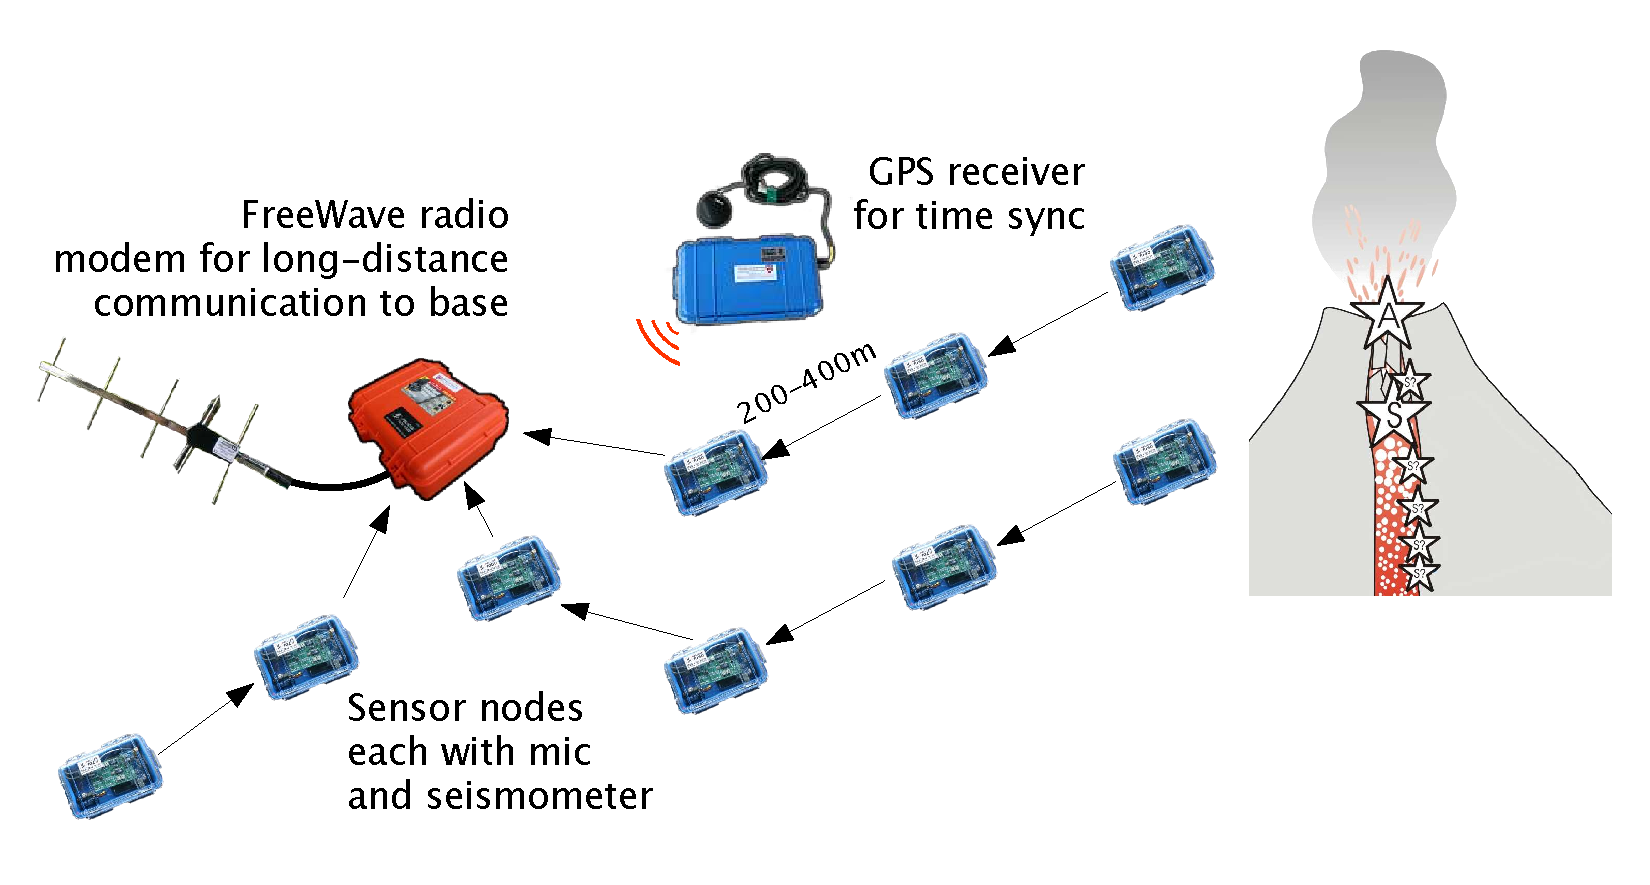
\includegraphics[width=0.7\hsize]{./5-evaluation/figs/schematic}
\end{center}
\caption{\textbf{Schematic representation of our sensor network
architecture.}}
\end{figure}

A single sensor network node, interface board, and battery holder were all
housed inside a small weatherproof and watertight Pelican case.  We installed
environmental connectors through the case allowing cables to external sensors
and antennae to be attached without opening the case and disturbing the
equipment inside.  When working in wet and gritty conditions these became a
tremendous asset.

\begin{figure}[t]
\begin{center}
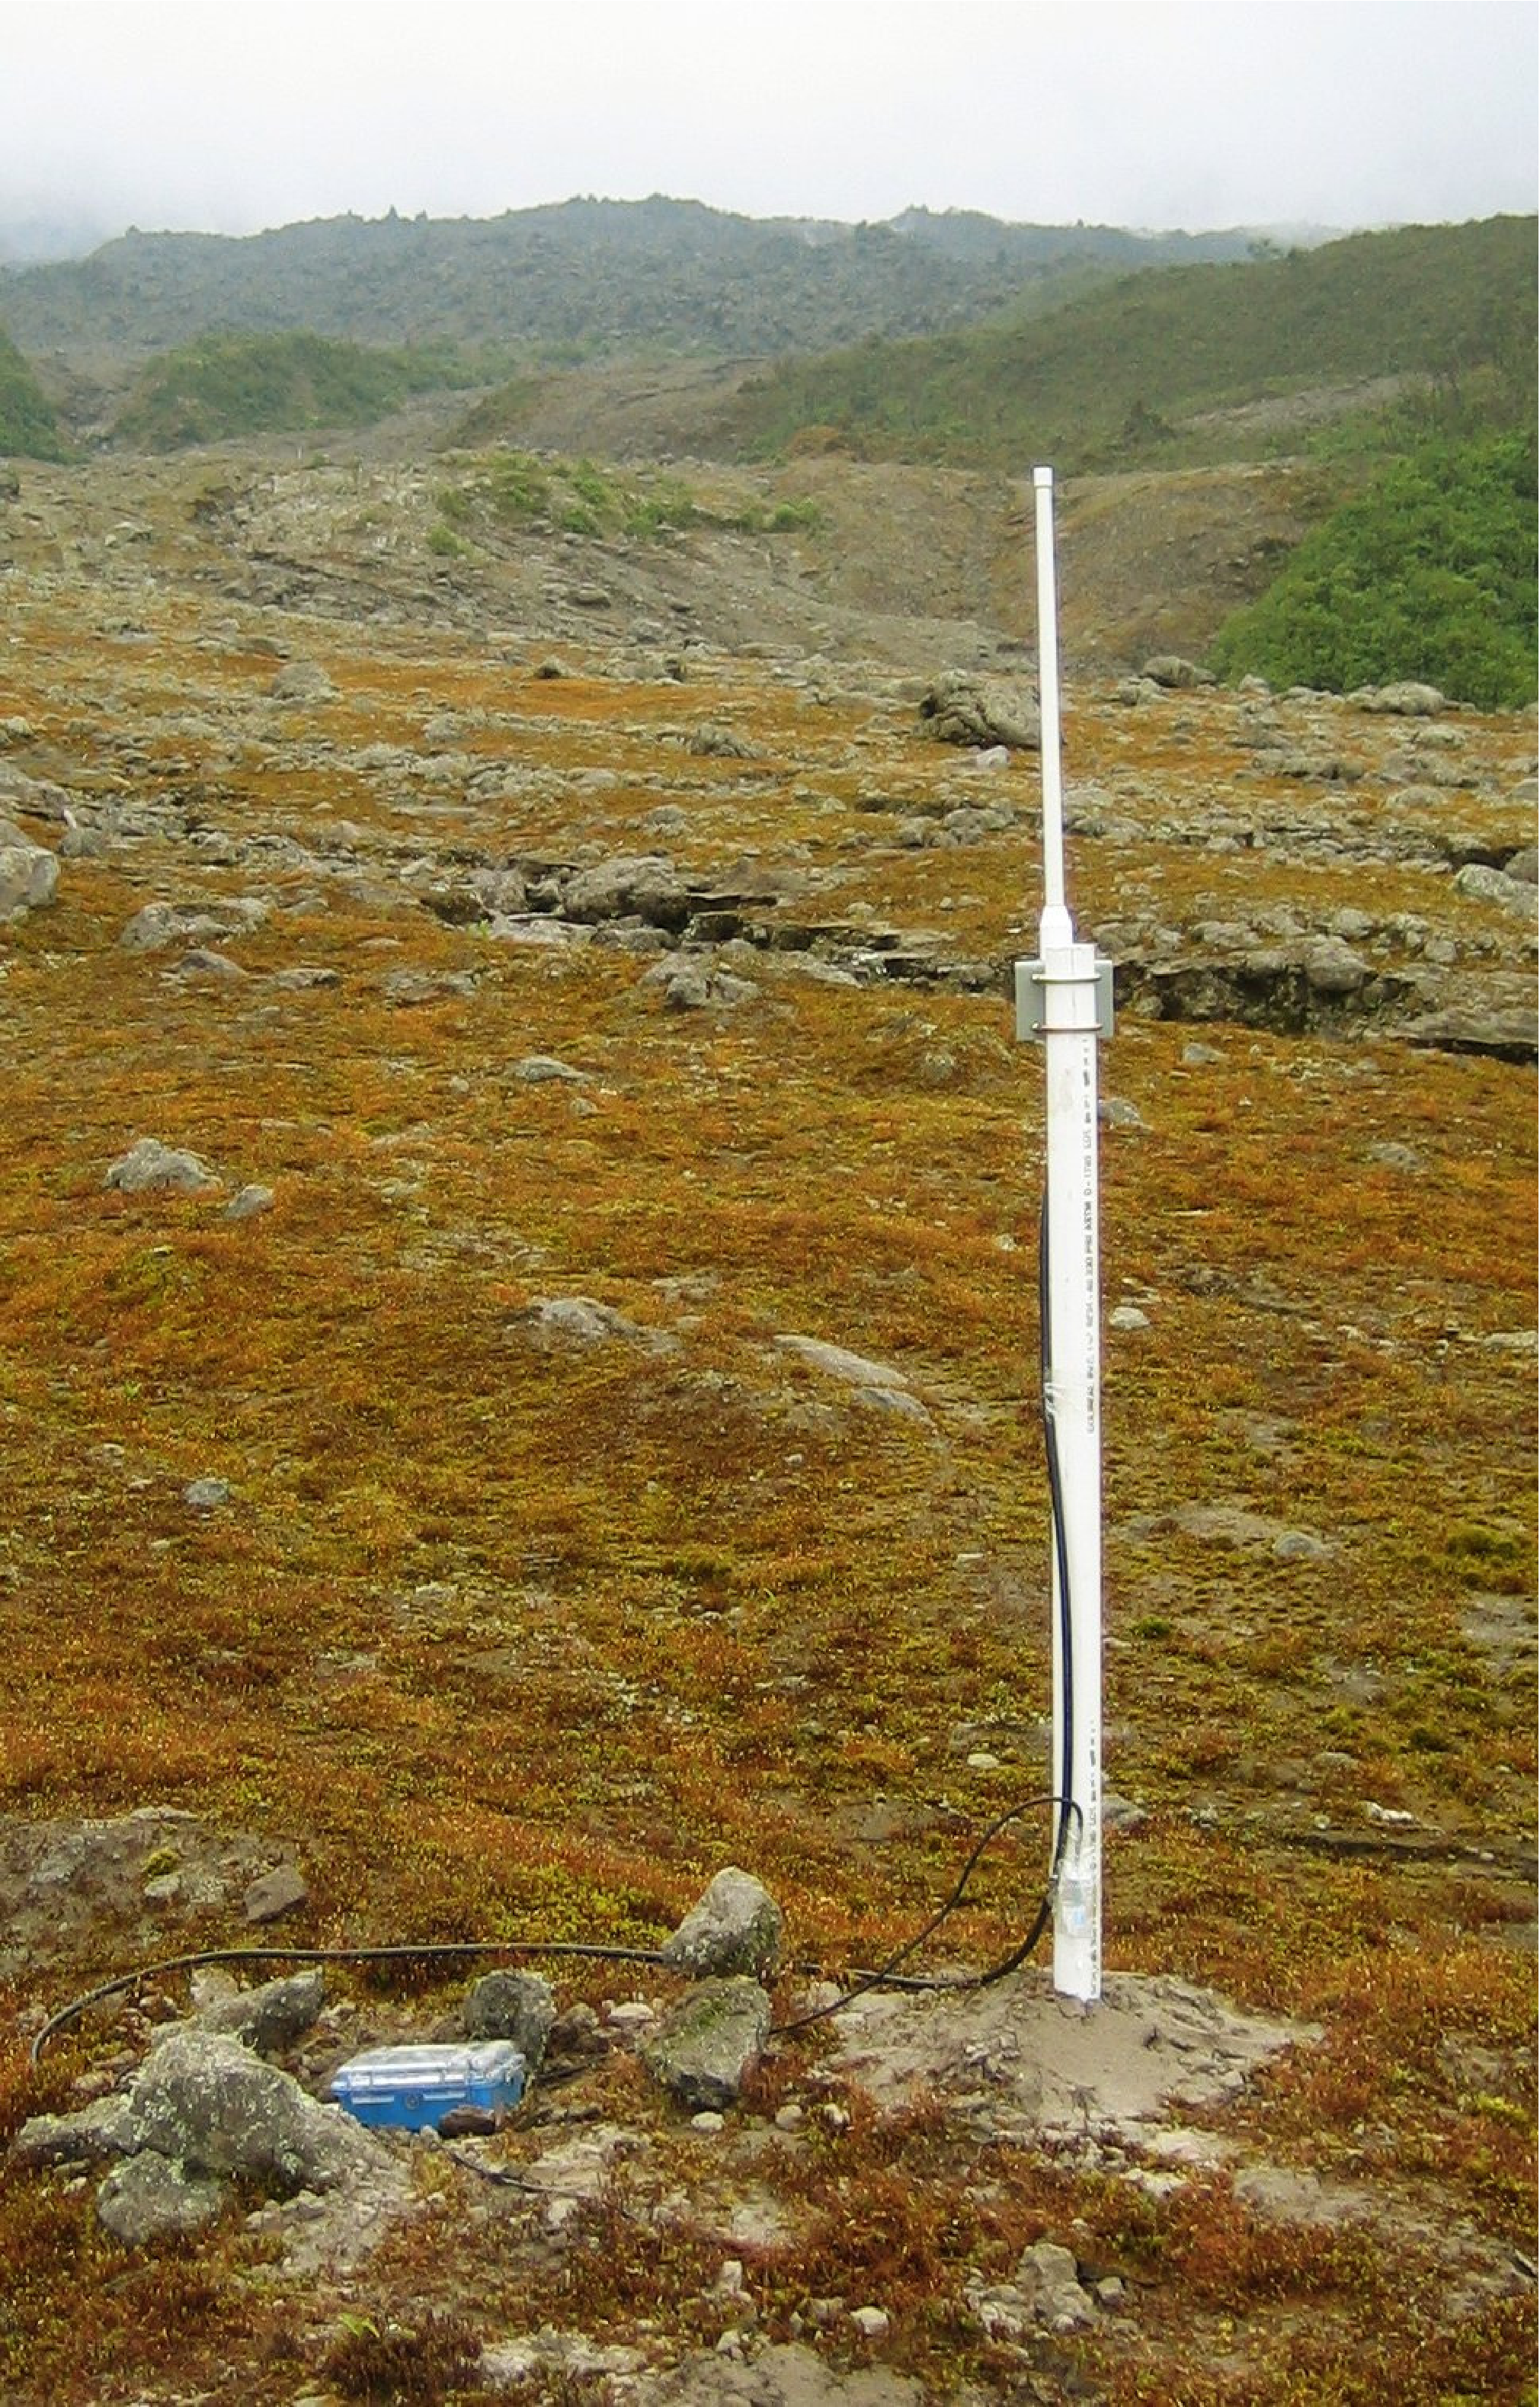
\includegraphics[width=0.7\hsize]{./5-evaluation/figs/Station}
\end{center}
\caption{\textbf{One of our two-component stations.  The blue Pelican
Case contains the wireless sensor network node and hardware interface board.
The external antenna is mounted on the PVC pole to reduce ground effects.
A microphone is taped to the PVC pole and a single seismometer is buried
nearby.}}
\label{fig-station}
\end{figure}

Installing a station involved covering the Pelican case with rocks to anchor
it and shield the contents from direct sunlight.  Cables were run from the
box to each sensor and to the antenna.  The antenna was elevated on a 1.5~m
length of PVC piping to reduce ground effects which reduce radio range.  The
seismometers were buried nearby, but far enough away to remain undisturbed by
any wind-induced shaking of the antenna pole.  The microphone was usually
mounted on the antenna pole and shielded from the wind and elements with
plastic tape.  Installation took a matter of minutes and the equipment was
sufficiently light and small that six stations could be carried in a large
pack.  The PVC poles were light but bulky and proved the most awkward part of
each station to cart around.

\subsection{Network Location and Topology}

We installed our stations in a roughly linear configuration, radiating away
from the vent and producing an aperture of over 3~km.  We attempted to
position the stations as far apart as the radios on each node would allow.
Although our antennas could maintain radio links of over 400~m, the geography
at the deployment site occasionally required installing additional stations
to maintain radio connectivity.  Other times we would deploy a node expecting
it to communicate with an immediate neighbor but later notice that that node
was bypassing its closest companion in favor of a node closer to the base
station.  Most nodes communicated with the base station over three or fewer
hops, but a few were moving data over as many as six.

In addition to the sensor nodes, several other pieces of equipment
were used.  Three Freewave~\cite{freewave} radio modems provided a
long-distance, reliable radio link between the sensor network and the
observatory laptop.  Freewave modems at the deployment site and the
observatory used a 9~dBi directional Yagi antenna to relay data via a
repeater station, installed on a hill with good line-of-sight to both
endpoints.  Each Freewave required a car battery for power, recharged
by solar panels.  A small number of Crossbow~\cite{xbow} MicaZ sensor
network nodes served in supporting roles.  One interfaced between the
network and the Freewave modem; another was attached to a GPS receiver
to provide a global timebase.

\begin{figure}[t]
\label{includegraphics-fig-plot}
\begin{center}
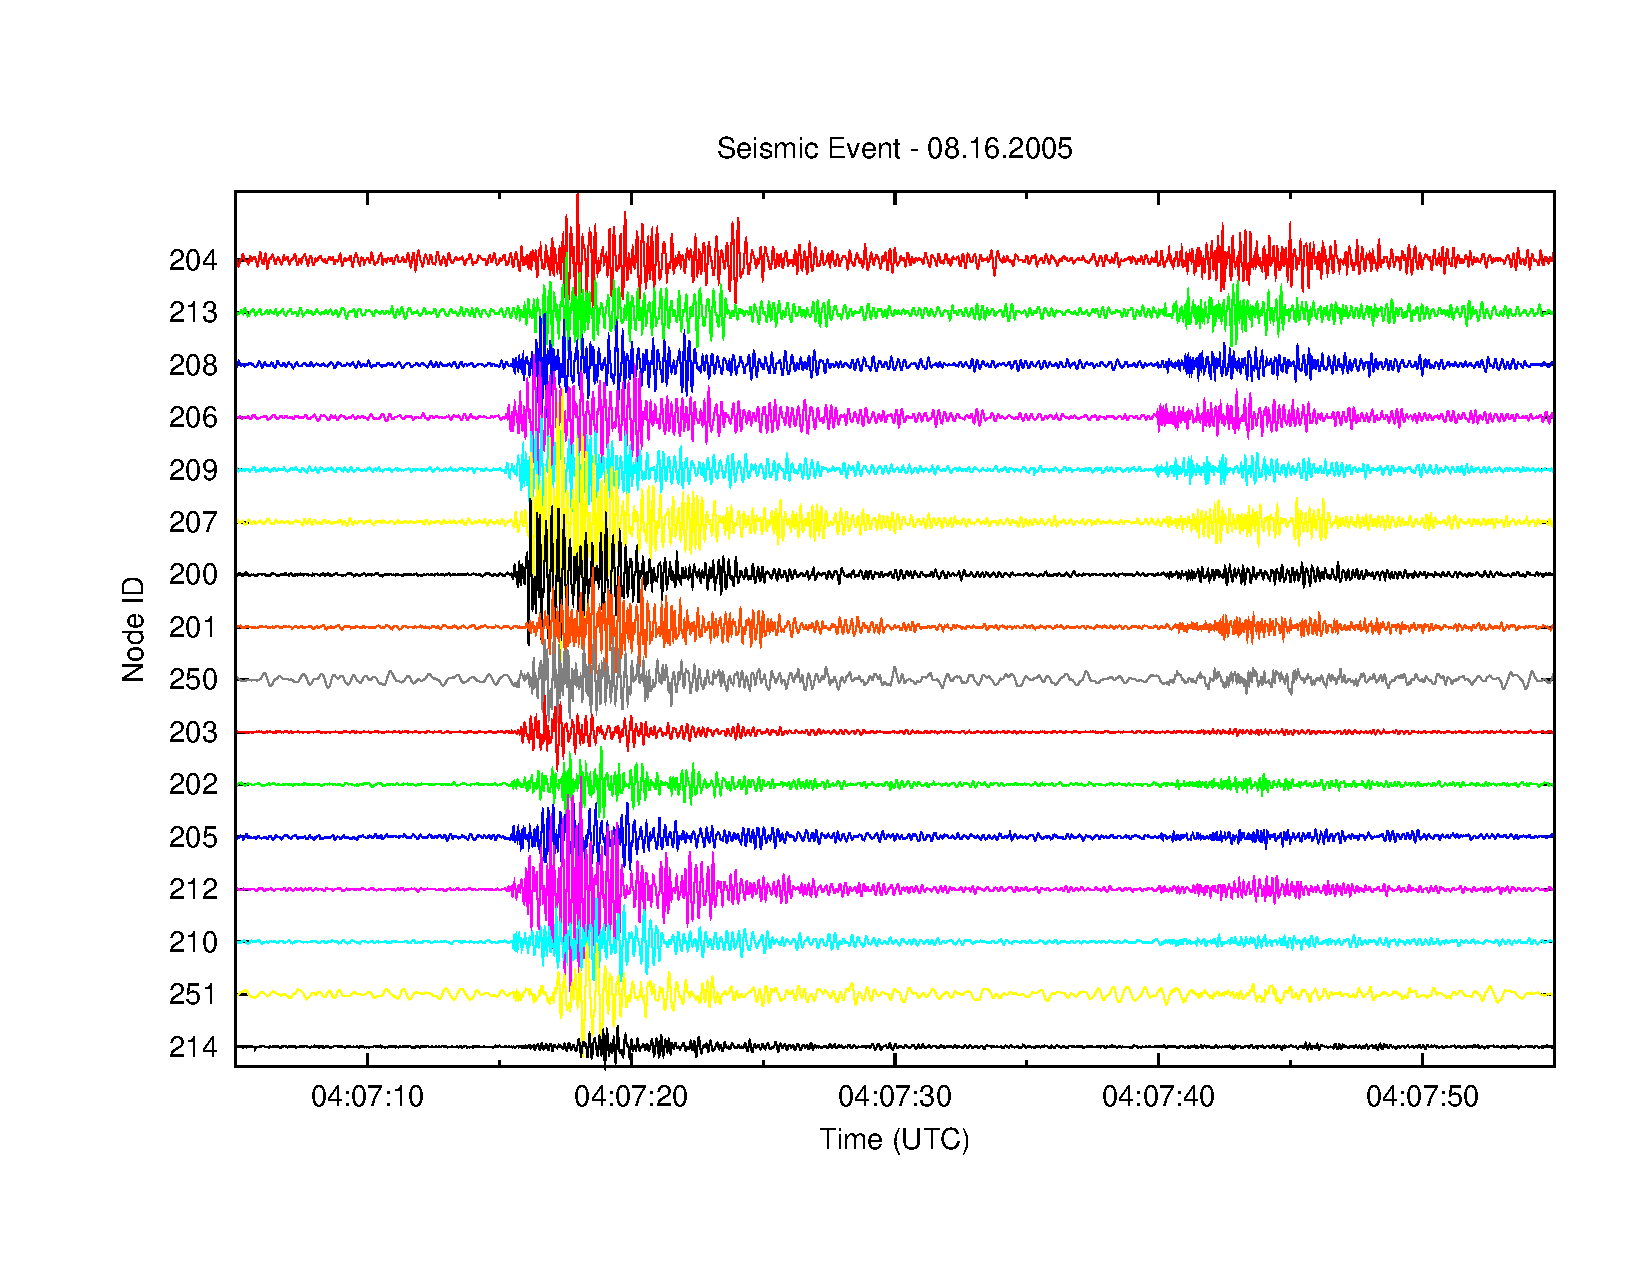
\includegraphics[width=0.7\hsize]{./5-evaluation/figs/TEST}
\end{center}
\caption{\textbf{Example of an event captured by our network.}  Only
seismic signals are shown.  The event shown was a Volcano Tectonic (VT) event
and had no interesting acoustic component.  Data shown has undergone several
rounds of post-processing including mapping to GMT time.}
\end{figure}

\begin{figure}[t]
\begin{center}
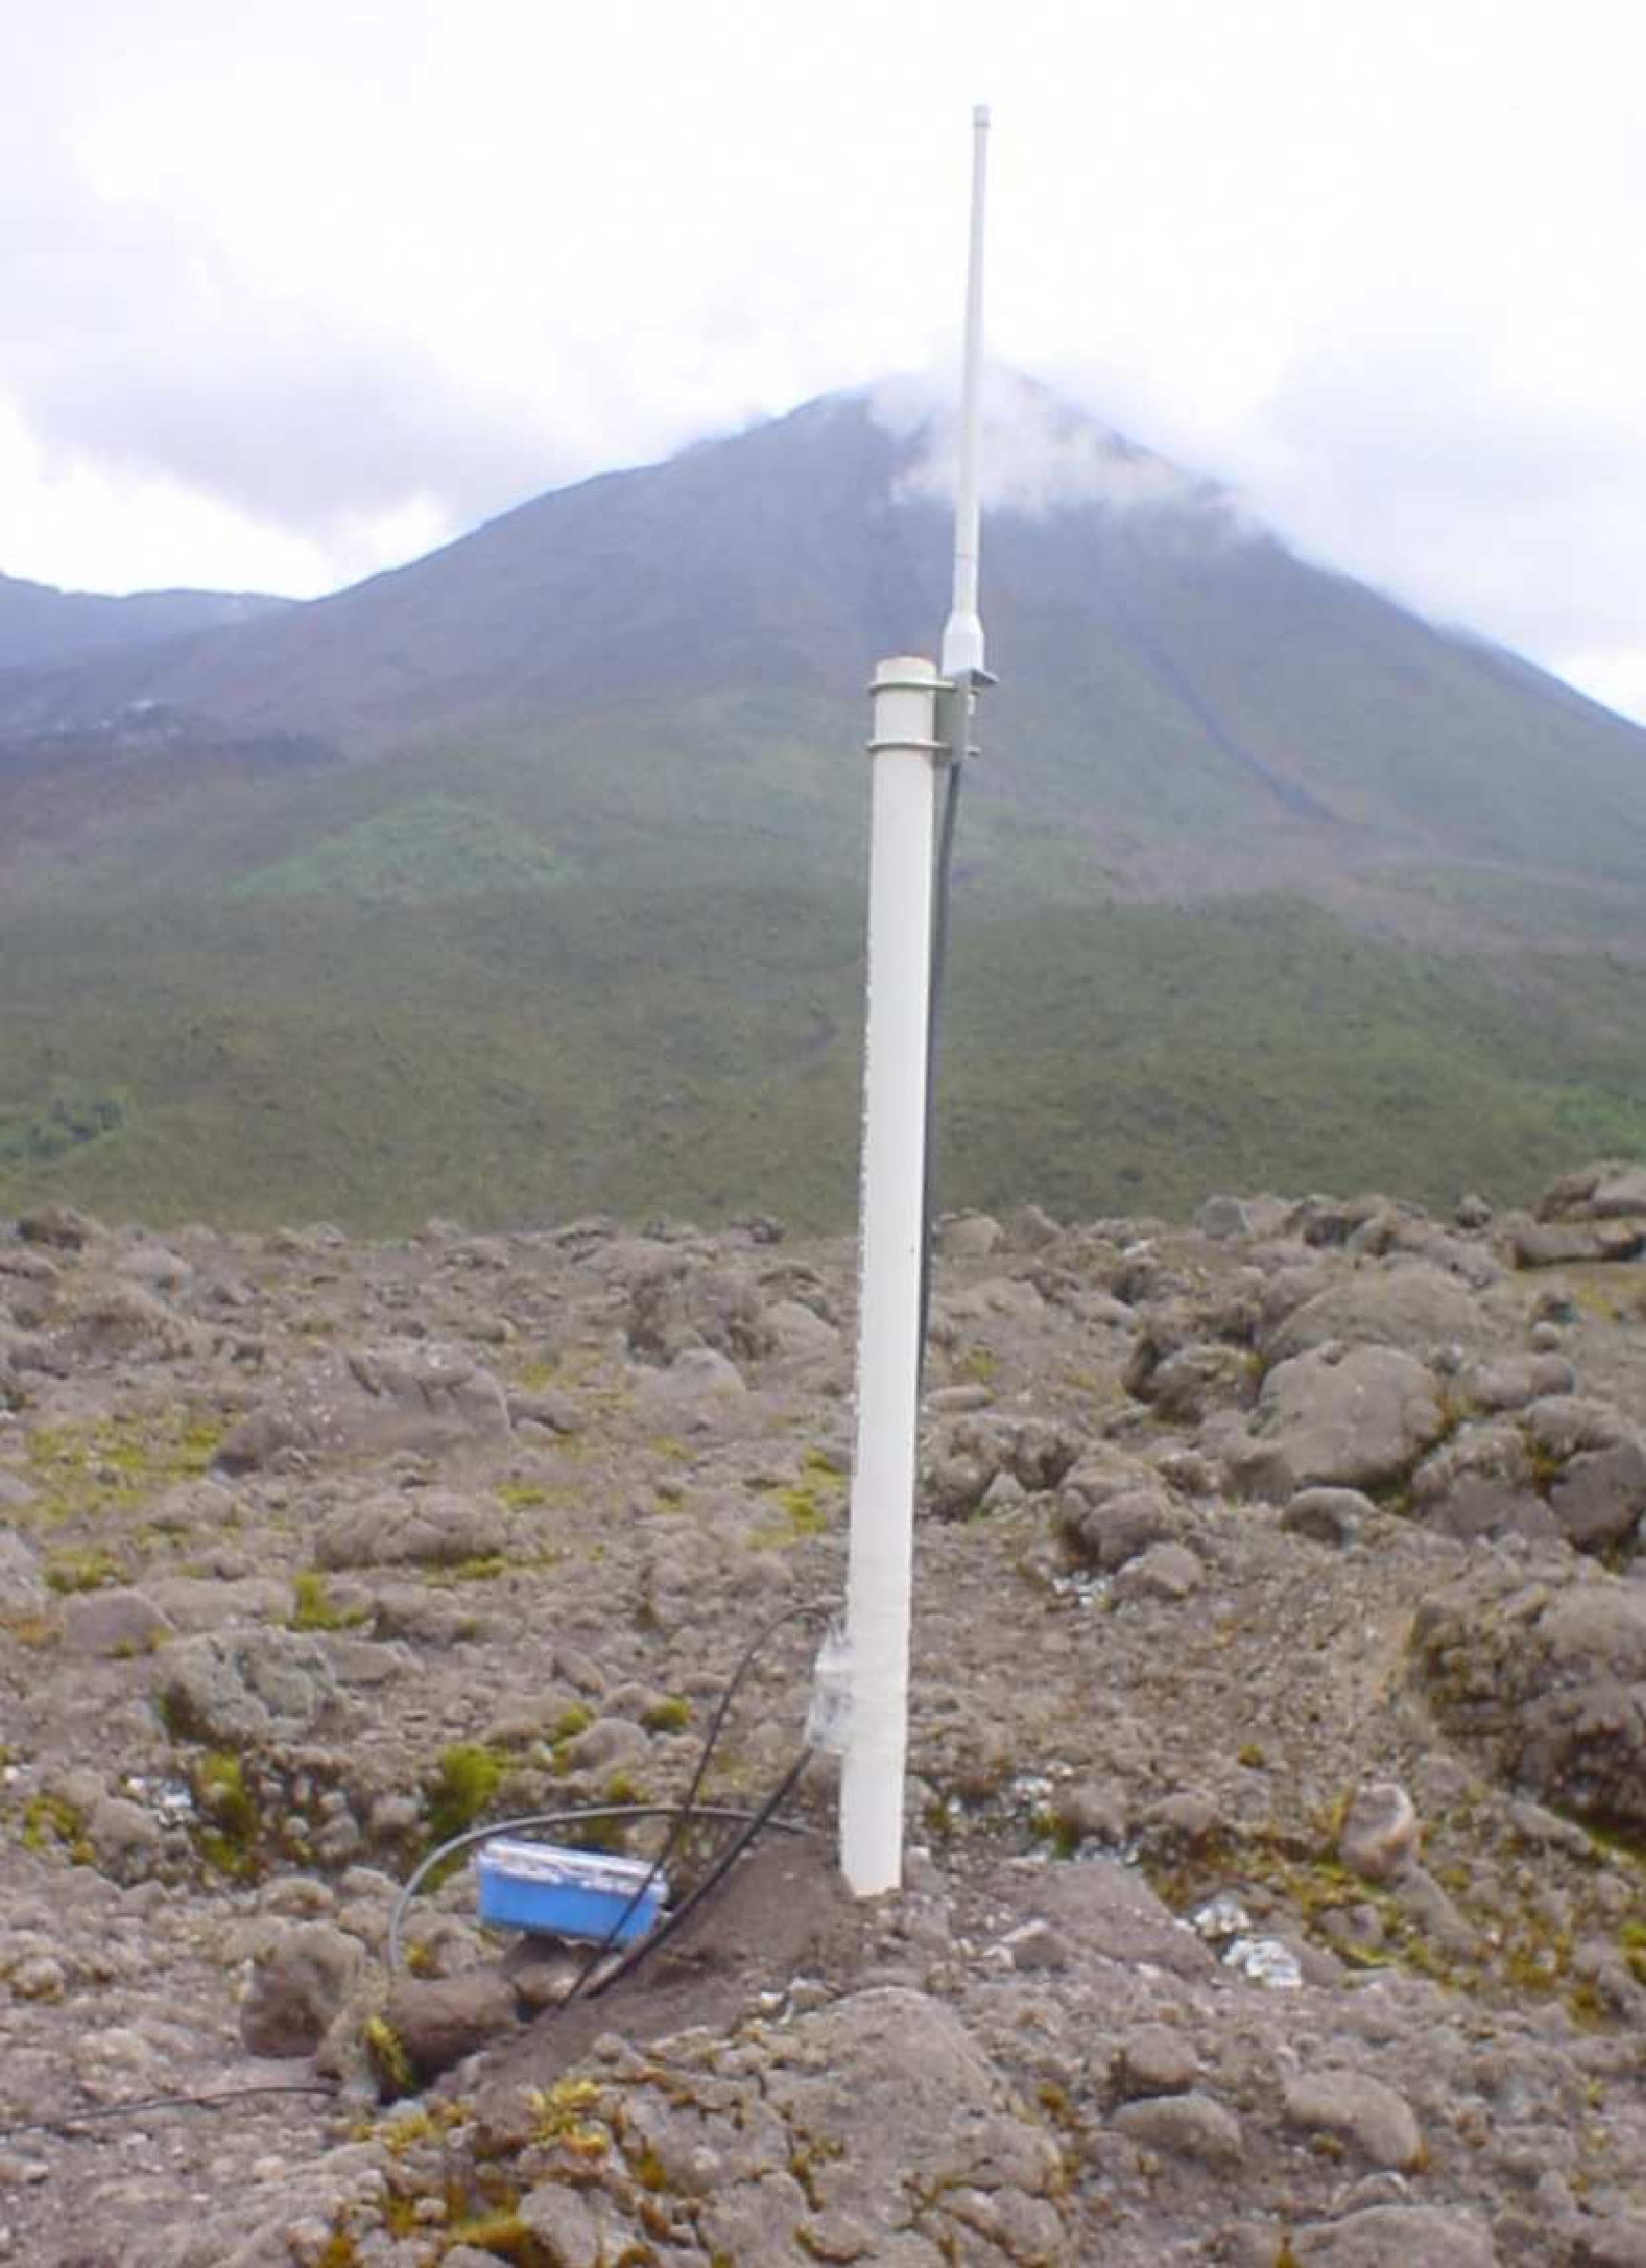
\includegraphics[width=0.7\hsize]{./5-evaluation/figs/Node-212-5}
\end{center}
\caption{\textbf{One of our two-component stations.} The blue Pelican
Case contains the wireless sensor network node and hardware interface board.
The external antenna is mounted on the PVC pole to reduce ground effects.
A microphone is taped to the PVC pole and a single seismometer is buried
nearby.}
\label{includegraphics-fig-station2}
\end{figure}

\XXXnote{GWA: Pulled from OSDI'06 design.}

\subsection{Sensor hardware}
\label{evaluation-sec-hardware}

\begin{figure}[t]
\label{evaluation-fig-station}
\begin{center}
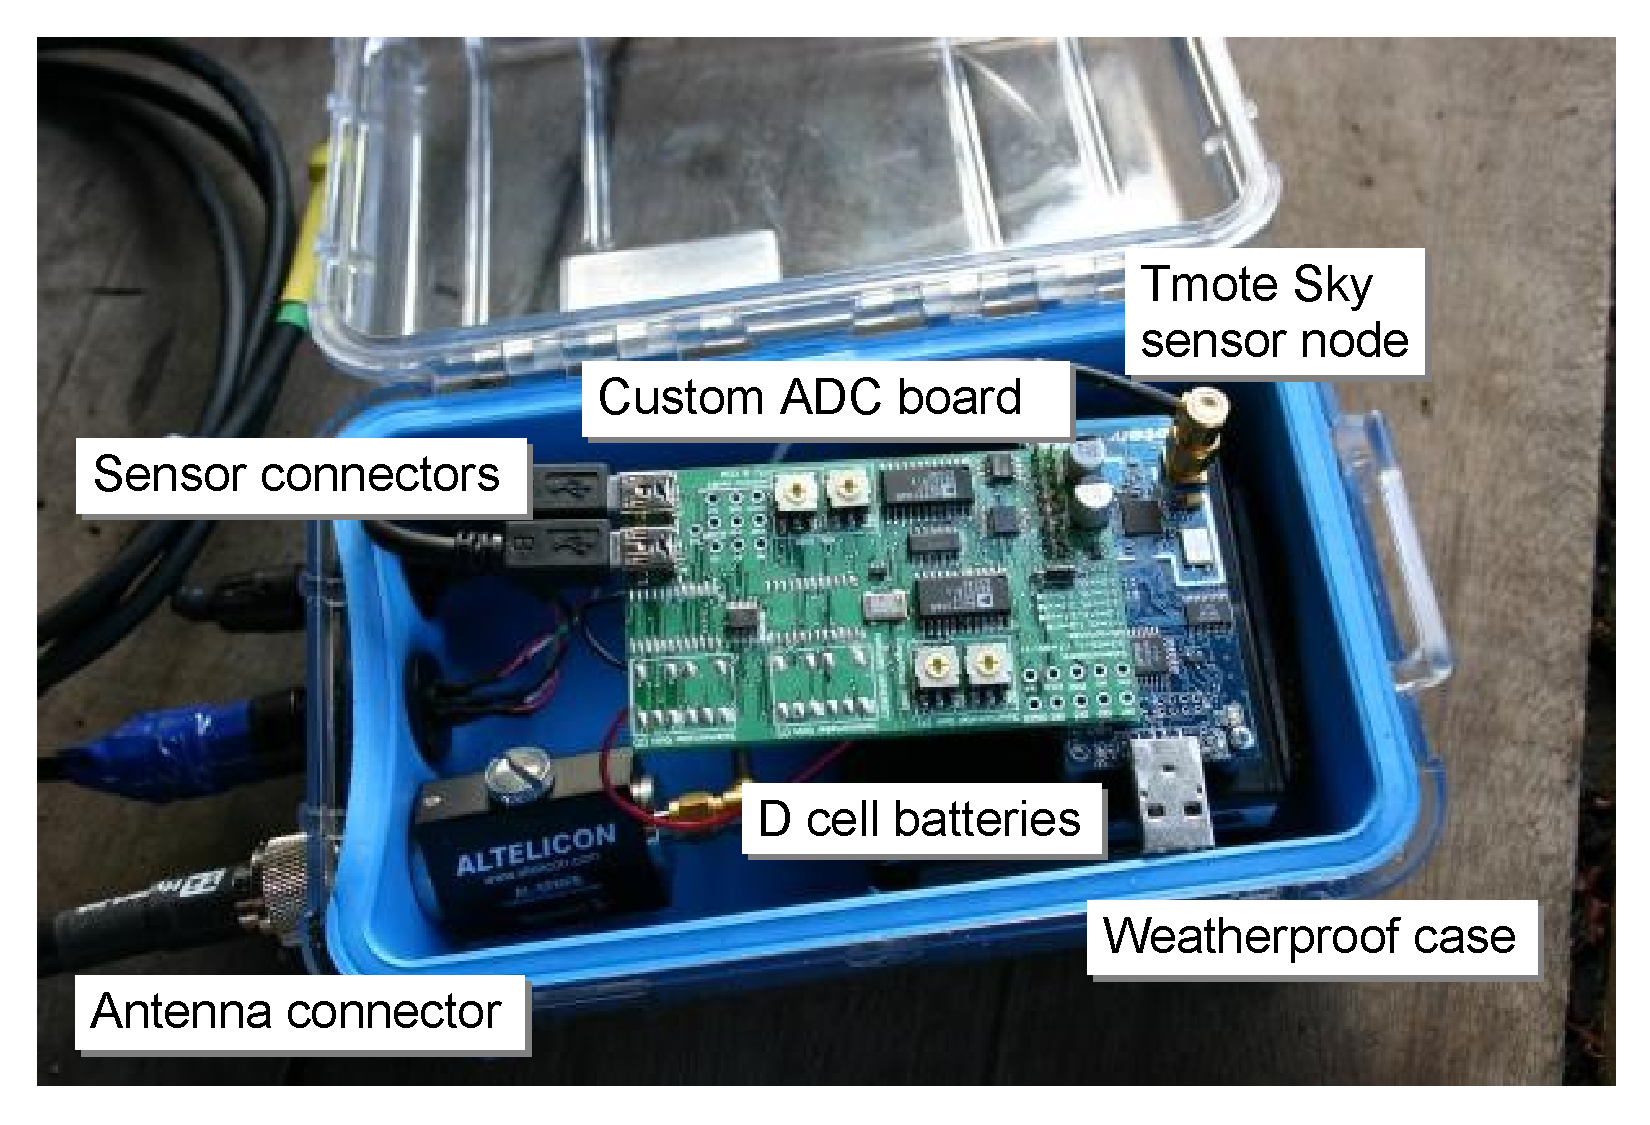
\includegraphics[width=1.0\hsize]{./5-evaluation/figs/Station2-small.pdf}
\end{center}
\caption{\textbf{Our wireless volcano monitoring sensor node.}}
\end{figure}

%We deployed 16 wireless monitoring stations onto Volc\'{a}n Reventador.
%Nodes were arranged in a roughly-linear configuration radiating from the vent
%and spanning over 3km.  Figure REFERENCE shows the locations of each node as
%well as those of several wired monitoring stations deployed nearby.
%\GWAnote{Do we event want to include this figure again? It takes up a lot of
%space but it probably would be nice to have...}

Our wireless sensor node (Figure~\ref{evaluation-fig-station}) is based on
the TMote Sky~\cite{moteiv} platform, which integrates a TI~MSP430 processor,
10~KB of SRAM, 48~KB of program ROM, 1~MByte of flash memory, and a Chipcon
CC2420 radio. All software is implemented in TinyOS~\cite{tinyos-asplos00}.
We designed a custom sampling board that provides four channels of 24-bit
analog-to-digital conversion (TI~AD7710). 
%While the MSP430 provides several channels of ADC, its resolution of 16~bits
%was inadequate for our needs.

Nodes were interfaced to either a single-axis seismometer (GeoSpace GS-11) or
three seismometers in a triaxial configuration (GeoSpace GS-1). 
%The GS-11 sensors are inexpensive and lightweight, but are only sensitive at
%frequencies above 4.5~Hz. In contrast, the GS-1 sensors have a corner
%frequency of 1~Hz but are significantly more expensive and heavy. 
Both sensors are passive instruments; ground motion generates a voltage which
is amplified and digitized by the sampling board.  In addition, each node was
attached to an omnidirectional microphone (Panasonic WM-034BY). This
microphone has been used in other infrasonic monitoring
studies~\cite{johnson-etal-04b}.

% MDW: Node 204 talked to 206 which was 1055 meters away!
Each node was equipped with an 8.5~dBi omnidirectional antenna mounted on
1.5~m of PVC pipe.  This permitted line-of-sight radio range of over 1~km
without amplification; nodes were typically placed 200-400~m apart in our
deployment. Nodes were powered by two D-cell batteries with a lifetime of
approximately 1~week.  Each node was enclosed in a weatherproof Pelican case.

Several other pieces of hardware complete the system. FreeWave radio modems
provided a long-distance radio link between the sensor array and the volcano
observatory, 4.6~km away. A laptop located at the observatory logged data and
was used to monitor and control the network.  Finally, to establish a global
timebase, we used a single Crossbow MicaZ~\cite{xbow} mote interfaced to a
GPS receiver (Garmin OEM~18~LVC).  The GPS receiver provided a 1~Hz pulse
that is accurate to GPS time within 1~$\mu$s, and acted as the root of the
network time synchronization protocol.
%as described in Section~\ref{evaluation-sec-timing}.

\subsection{Network topology and status monitoring}

Nodes form a multihop routing tree rooted at the gateway node that is
physically attached to the FreeWave modem; we use a variant of
MintRoute~\cite{awoo-multihop} that uses the CC2420's Link Quality Indicator
metric to select routing paths. Each node transmits a {\em status message}
every 10~sec that includes its position in the routing tree, buffer status,
local and global timestamps, battery voltage, and other information. 
%These status messages form the basis of much of the analysis in this paper.
In addition, the base station can issue a {\em command} to each node,
instructing it to respond with an immediate status message, start or stop
data sampling, and set various software parameters.  Commands are propagated
using a simple flooding protocol.  The {\em Deluge} protocol~\cite{deluge}
was also used to permit over-the-air reprogramming and rebooting of nodes.

\subsection{Event detection and data collection}

Because of the high data rates involved (600-1200~bytes/sec from each node)
it is infeasible to continuously transmit all sensor data. Rather, nodes are
programmed to locally detect interesting seismic events and transmit event
reports to the base station. If enough nodes trigger in a short time
interval, the base station attempts to download the last 60~sec of data from
each node.  This design forgoes continuous data collection for increased
resolution following significant seismic events, which include earthquakes,
eruptions, or long-period (LP) events, such as tremor.  The download window
of 60~sec was chosen to capture the bulk of the eruptive and earthquake
events, although many LP events can exceed this window (sometimes lasting
minutes or hours).  To validate our network against existing scientific
instrumentation, our network was designed for high-resolution signal
collection rather than extensive in-network processing.
%In the future we would like to explore more advanced in-network signal
%processing.

During normal operation, each node continuously samples its seismic and
acoustic sensors at 100~Hz, storing the data to flash memory. Data is stored
as 256-byte {\em blocks} in the flash.
%with each block identified by a monotonically increasing {\em block ID}.
Each block 
%is tagged with its ID 
is tagged with the {\em local timestamp} corresponding to the first sample in
the block.  This timestamp is later mapped onto a global time reference.
%as described in Section~\ref{evaluation-sec-timing}.
The 1~Mbyte flash is treated as a circular buffer storing approximately
20~min of data. 

In addition, nodes run an {\em event detection algorithm} that computes two
exponentially-weighted moving averages (EWMA) over the input signal with
different gain settings. When the ratio between the two EWMAs exceeds a
threshold, the node transmits an event report to the base station.
%$\alpha_{\mathit{high}} > \alpha_{\mathit{low}}$.  That is, the high-gain
%EWMA is more sensitive to changes in the input signal than the low-gain
%EWMA. If the ratio of the high-gain EWMA to the low-gain EWMA exceeds a
%threshold $T$, the node considers the signal to contain a significant event
%and transmits a {\em trigger} message to the base station.
If the base station receives triggers from 30\% of the active nodes within a
10~sec window, it considers the event to be well-correlated and initiates
data collection.

Our reliable bulk-transfer protocol, called {\em Fetch}, operates as follows.
The base station waits for 30~sec following an event before iterating through
all nodes in the network. The base sends each node a command to temporarily
stop sampling, ensuring the event will not be overwritten by subsequent
samples.  For each of the 206~blocks in the 60~sec window, the base sends a
{\em block request} to the node.  The node reads the requested block from
flash and transmits the data as a series of 8~packets.  After a short timeout
the base will issue a repair request to fill in any missing packets from the
block.
%The repair process continues until all packets have been received or a
%timeout occurs. 
Once all blocks have been received or a timeout occurs, the base station
sends the node a command to resume sampling and proceeds to download data
from the next node. 
%The data is logged by the base station laptop for later analysis.

\subsection{Deployment on Volc\'{a}n Reventador}

\begin{figure}[t]
\label{evaluation-fig-schematic}
\begin{center}
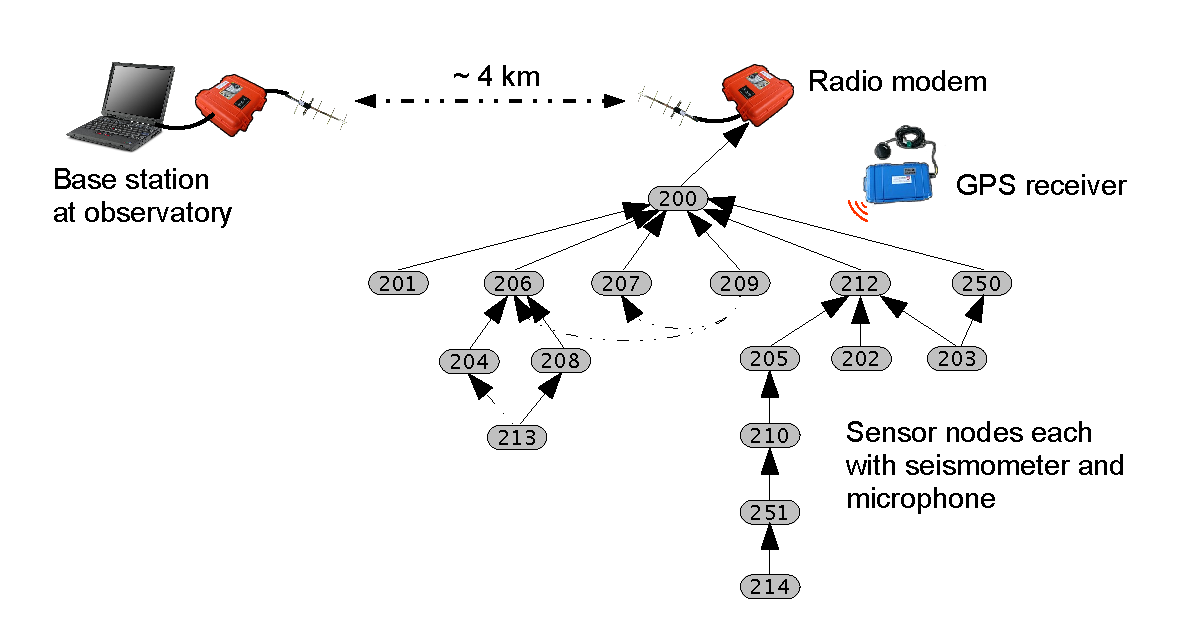
\includegraphics[width=1.0\hsize]{./5-evaluation/figs/schematic2.pdf}
\end{center}
\caption{\textbf{Sensor network architecture.} Nodes form a
multihop routing topology, relaying data via a long-distance radio
modem to the observatory. A GPS receiver is used to establish a global
timebase. The network topology shown here was used during
our deployment at Reventador.}
\end{figure}

\begin{figure}[t]
\label{evaluation-fig-map}
\begin{center}
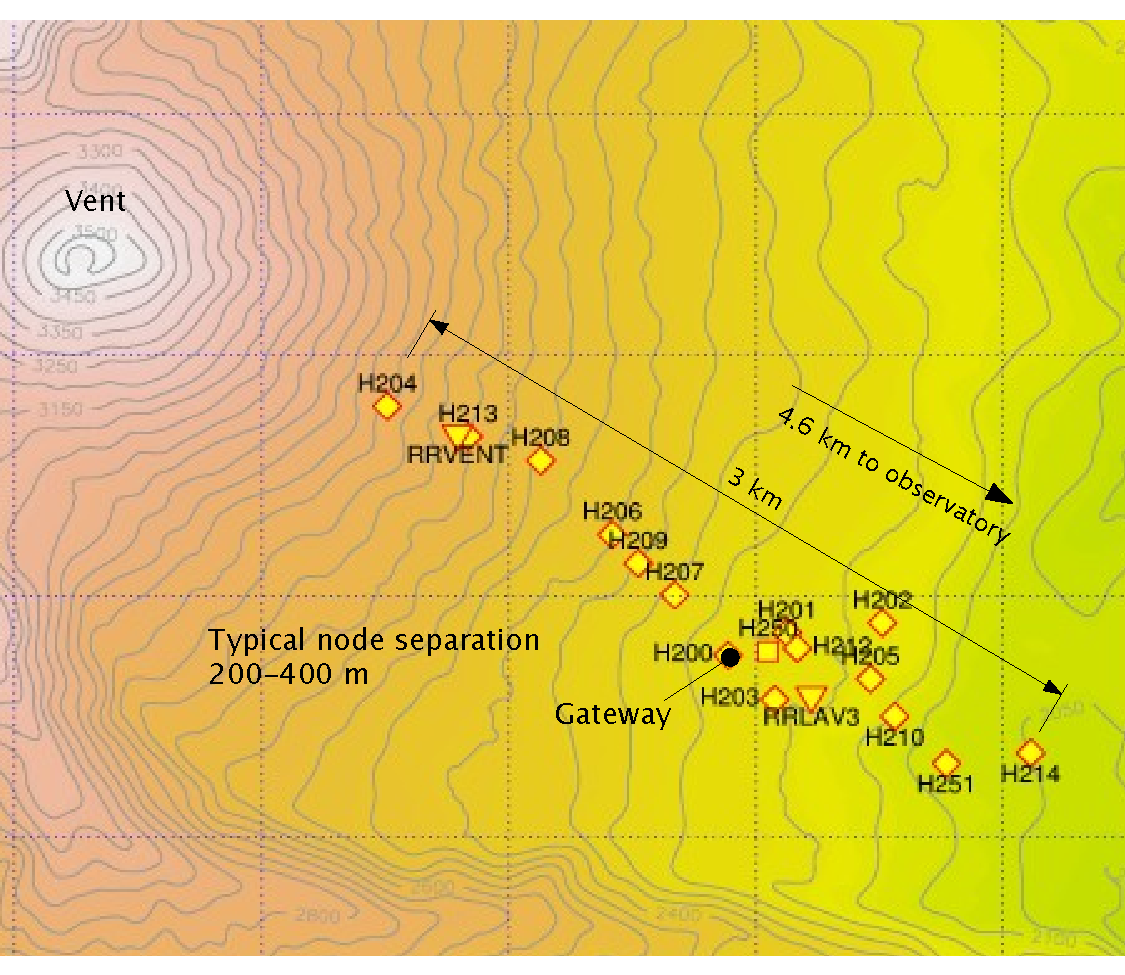
\includegraphics[width=1.0\hsize]{./5-evaluation/figs/reventador-map-crop.pdf}
\end{center}
\caption{\textbf{Map of sensor deployment at Volc\'{a}n Reventador.}
In addition to the 16~sensor nodes, two broadband seismometers
with data loggers (RRVENT and RRLAV3) were colocated with the network.}
\end{figure}

% MDW 26-Aug-06: I have revisited some of Jeff Johnson's suggestions
% in the below text; i.e., hyphenation on "broad-band" and so forth.

Our deployment at Reventador took place between August 1--19, 2005.
Reventador is an active volcano located in northern Ecuador, about 100~km
from Quito. 
%The volcano erupted with massive force in 2002, blanketing the streets of
%Quito with ash, closing schools and the airport. 
During this time, Reventador's activity consisted of small explosive events
that ejected ash and incandescent blocks several times a day. Associated
seismicity included numerous explosion earthquakes as well as
extended-duration shaking (tremor) and shallow rock-fracturing earthquakes.

We deployed 16~sensor nodes on the upper flanks of Reventador, as shown in
Figure~\ref{evaluation-fig-map}, over a 3~km linear configuration radiating
away from the vent. The resulting multihop topology is shown in
Figure~\ref{evaluation-fig-schematic}. The upper flanks of the volcano were
completely deforested by a large eruption in November 2002, allowing for
line-of-sight radio communication between adjacent sensor nodes.  Two
standalone seismic stations, consisting of a broadband sensor, a Reftek 130
data logger with 1~GByte flash memory cards, and a GPS receiver for
timestamping, were colocated with sensor nodes. The data from these stations
is essential to our network validation.
%described in
%Sections~\ref{evaluation-sec-eventdetection}~and~\ref{evaluation-sec-timing}.
The base station was located at a small hotel 4.6~km from the deployment
site.  The sensors were deployed for a total of 19~days, during which time
the network recorded data from 229~earthquakes, eruptions, and tremor events,
logging 107~MBytes of data. The long hike and lack of roads prevented
frequent returns to the deployment site, although we returned several times
to change batteries and perform other network maintenance.

%Colocated with our
%sensor network were two broadband seismometer stations,
%each using a Reftek~130 data logger with 1~GByte flash memory cards
%and a GPS receiver for timestamping. The data from these stations 
%is essential to our network validation, described in 
%Sections~\ref{sec-eventdetection}~and~\ref{sec-timing}.  
%The base station was located at 
%a small hotel 4.6~km from the deployment site. 

% MDW 26-Aug-06: I don't think this subsection is really needed. 
% Maybe the first paragraph could be added back somewhere; the rest is
% not pithy enough to warrant inclusion.

%\subsection{Design decisions}
%
%For this deployment our primary design goals were simplicity,
%statelessness, and robustness.  As such, we chose not to focus on
%aggressive power management, routing performance, fault tolerance
%(e.g. multiple base stations and GPS receivers), or scalability.  We
%plan to address these issues in future deployments.
%
%Some of our design decisions were influenced by the fact that the deployment
%site was a strenuous 3~hour hike from the observatory, meaning that we wanted
%to avoid problems that might require returning to the deployment
%site.  Other decisions were driven by more pragmatic reasons.  For example,
%although having a GPS receiver on each node would make the system more
%robust, we decided against it due to the increased cost, power, and
%deployment logistics.  Each GPS node requires a car battery to power it for a
%longer duration, making the deployment impractical given the difficult
%circumstances.  Instead we decided to equip only one node with a GPS receiver
%and use FTSP~\cite{ftsp} to synchronize the rest of the network.
%
%Finally, we point out that initially we planed on a 25~node network.
%However, because of various hardware failures we ended up with 16
%deployable nodes.


\section{Sensor Network Application Design}
\label{sec-cs}

Given the current capabilities of wireless sensor network nodes, we set out to
design a data collection network meeting the scientific requirements outlined
above.  Before motivating our design we provide a high-level overview of
network operation.

\subsection{Typical Network Operation}

Each node samples two or four channels of seismoacoustic data at 100~Hz,
storing the data in local flash memory. Nodes also transmit periodic status
messages and perform time synchronization, as described below.
When a node detects an interesting event, it routes a message to the 
base station laptop.  
If enough nodes report an event within a short time interval, the laptop
initiates data collection which proceeds in a round-robin fashion. Between
30~and~60~seconds of data is downloaded from each node with a reliable data
collection protocol, ensuring that all buffered data from the event is
retrieved.  When data collection completes, nodes return to sampling 
and storing sensor data.

\subsection{Overcoming High Data Rates: Event Detection and Buffering}

% GWA : Changed numbers to KBS and fixed 50 Kbits/second number which is
% lowballing it.

When designing high data-rate sensing applications the most important
limitation of current sensor network nodes is low radio bandwidth.  IEEE
802.15.4 radios, such as the Chipcon CC2420, have raw data rates of around
30~KBytes/sec.  However overheads caused by packet framing, medium access
control (MAC), and multihop routing reduce the achievable data rate to less
than 10~KBytes/sec even in a single-hop network.

As a result, nodes can acquire data faster than they can transmit.  Simply
logging data to local storage for later retrieval is also infeasible for
these applications.  The TMote Sky has 1~MByte of flash memory which fills in
around 20 minutes on a two-component sensor node.  Fortunately, many
interesting volcanic events will fit in this buffer.  For a typical
earthquake or explosion at Reventador, 60~sec of data from each node is
adequate.  Therefore, we focused on developing a network to reliably collect
data for short, discrete events.  

% MDW: I don't think we need to use the term "local" event detector
% here. Also, you only need to italicize a term the first time it is
% used.
Sampled data is stored in the local flash memory of the node, which is
treated as a circular buffer. Each block of data is timestamped using
the local node time, which can later be mapped onto a global time,
as explained below. Each node runs an {\em event detector} on 
locally-sampled data. 
Good event detection algorithms produce high
event-detection rates while maintaining small false-positive rates.
The sensitivity of the detection algorithm links these two metrics: a more
sensitive detector correctly identifies more events at the
expense of producing more false positives.  

The data set produced by our previous deployment at Volc\'{a}n
Tungurahua~\cite{volcano-ewsn05} aided in the design of the event detector.
We implemented a short-term average/long-term average threshold detector,
which computes two exponentially-weighted moving averages (EWMAs) with
different gain constants. When the ratio between short-term average and the
long-term average exceeds a fixed threshold, the detector fires.  The
detector threshold allows nodes to distinguish between low-amplitude signals,
perhaps caused by distant earthquakes, and high-amplitude signals caused by
nearby volcanic activity.

When the event detector on a node fires it routes a small message to the base
station laptop.  If enough nodes report events within a certain time window
the laptop initiates data collection from the entire network (including nodes
that did not report the event). This global filtering prevents spurious event
detections from triggering a data collection cycle. Fetching 60~sec of data
from all 16 nodes in the network takes approximately one hour.  Because nodes
can only buffer 20 minutes of eruption data locally each node pauses sampling
and reporting events until its data has been uploaded.  As the latency
associated with data collection prevents our network from capturing all
events, optimizing the data collection process is a focus of future work.

%Buffering on each node is required because the identification and data
%retrieval takes time after which data from an event must remain available on
%the node.  We developed a component allowing us to treat the Flash memory as
%circular buffer.  Because our nodes filled this store in roughly 20 minutes
%and it typically took around one hour to download a single event from the
%entire network we disabled sampling on each node before beginning the global
%retrieval process.  

% GWA : Found a lot of this confusing and bordering on incorrect.  Cleaned up
% a bit.

\subsection{Reliable Data Transmission and Time Synchronization}

% Konrad: Rewrote this paragraph. I think it's clearer now.
Extracting high-fidelity data from a wireless sensor network is
challenging for two primary reasons.  First, the radio links are lossy
and frequently asymmetrical.  Second, the low-cost crystal oscillators
on these nodes have low tolerances and therefore the clock rates vary
across the network.  Much prior research has focused on addressing
these challenges.

%% Extracting high-fidelity data from a sensor network means coping with lossy
%% radio links and accurately time-stamping sampled data.  Radio links in
%% wireless sensor networks are lossy and frequently asymmetrical, and low-cost
%% crystal oscillators deployed on wireless sensor network nodes have low
%% tolerances and clock rates vary across the network.  Much prior research has
%% focused on addressing these challenges.

% MDW: I found the fetch description to be somewhat confusing; tried
% to reorganize.

We developed a reliable data-collection protocol, called {\tt Fetch}, that
retrieves buffered data from each node over a multihop network. Samples are
buffered locally in {\em blocks} of 256~bytes, tagged with a sequence number
and timestamp. During transmission each requested block is fragmented into a
number of {\em chunks}, each sent in a single radio message. The base station
laptop retrieves a block by flooding a request to the network using {\tt
Drip}, a variant of the TinyOS {\tt Trickle}~\cite{trickle}
data-dissemination protocol.  The request contains the target node ID, the
block sequence number, and a bitmap identifying missing chunks in the block. 

The target node replies by sending the requested chunks over a multihop path
to the base station.  The routing tree is constructed using {\tt
MultiHopLQI}, a variant of the TinyOS {\tt MintRoute}~\cite{awoo-multihop}
routing protocol modified to select routes based on the CC2420 Link Quality
Indicator (LQI) metric.  Link-layer acknowledgments and retransmissions are
used at each hop to improve reliability.  Retrieving one minute of stored
data from a two-channel sensor node requires fetching 206~blocks and can
takes several minutes to complete, depending on the quality of the multihop
path and the node's depth in the routing tree.

% MDW: I think we paint too rosy of a picture here: we need to explain that
% FTSP does not always work lest the reader think we relied on it blindly,
% and point to future work.
Scientific volcano studies require that sampled data be accurately
timestamped; in our case, a global clock accuracy of 1~msec was sufficient.
We chose to use the Flooding Time Synchronization Protocol (FTSP)~\cite{ftsp}
from Vanderbilt University to establish a global clock across our network.
The published accuracy of FTSP is very high and the TinyOS code was
straightforward to integrate into our application. One of the nodes used a
Garmin GPS receiver to map the FTSP global time to GMT.  Unfortunately, FTSP
occasionally exhibited unexpected behavior which prevented nodes from
accurately timestamping some data. We are currently developing techniques to
correct the timestamps of our data set based on the large amount of status
messages logged from each node, which provide a mapping from the local clock
to the FTSP global time.
% MDW: This is a nice setup for your next paper...

\subsection{Command and Control}

% MDW: This is not universally true!
A feature missing from most traditional volcanic data acquisition equipment
is real-time network control and monitoring. The long-distance radio link
between the observatory and the sensor network allowed the laptop to monitor
and control the network's activity. We developed a Java-based GUI for
monitoring the network's behavior and manually setting parameters, such as
sampling rates and event detection thresholds.  In addition, the GUI was
responsible for controlling data collection following a triggered event,
moving significant complexity out of the sensor network.  All packets
received by the laptop from the sensor network were logged, facilitating
later analysis of the network's operation.

The GUI also displayed a table summarizing network state, based on the
periodic status messages transmitted by each node.  Each table entry included
the node ID; local and global timestamps; various status flags; the amount of
locally-stored data; depth, parent, and radio link quality in the routing
tree; and the node's temperature and battery voltage.  This functionality
greatly aided sensor deployment, as a team member could rapidly determine
whether a new node had joined the network and the quality of its radio
connectivity.


\section{Network Robustness}
\label{evaluation-sec-robustness}

The first evaluation metric that we consider is the {\em robustness} of the
sensor network.  Sensor network deployments have typically been plagued by
failures of individual nodes and the support infrastructure. Clearly,
robustness has a direct effect on the resulting data yield.  Our evaluation
shows that while nodes exhibited very high uptimes, the base station
infrastructure was very unreliable, and a single bug affecting the Deluge
protocol caused a three-day outage of the entire network.

%For example, in the 2003~Great Duck Island
%deployment~\cite{gdi-sensys04}, burrow nodes in the multihop network 
%failed after an average of 29~days, primarily due to battery
%exhaustion.

\subsection{Overall network uptime}

\begin{figure}[t]
\label{evaluation-fig-nodesalive}
\begin{center}
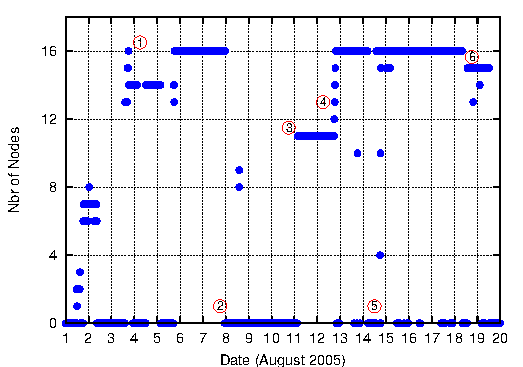
\includegraphics[width=\hsize]{./5-evaluation/figs/robustness/nodesalive/nodesalive.pdf}
\end{center}
\caption{\textbf{Nodes reporting over time.}
This figure shows the number of nodes reporting over each 10~min window
during the 19-day deployment period.  The annotations (1) through (6) are
described in the text.}
\end{figure}

Figure~\ref{evaluation-fig-nodesalive} shows the number of nodes reporting
over each 10-minute interval during the entire 19-day deployment. A node is
included in the count if any of its status messages were received at the base
station during the 10-minute window.  Annotations show several significant
events that occurred during the deployment. The network was installed in two
phases of 8~nodes each, the first on August~1 and the second on August~3.  At
label (1) the entire 16~node network is operational.  However, initial
software misconfiguration required rebooting several nodes during a third
visit to the deployment site on August~5.  The network then ran with 16~nodes
active for a little more than 2~days. 

At label (2) on August~8, a software command was transmitted to reboot the
network, using Deluge~\cite{deluge}, in an attempt to correct the time
synchronization fault described in Section~\ref{evaluation-sec-timing}.  This
caused a software failure affecting all nodes, with only a few reports being
received at the base station later on August~8.  After repeated attempts to
recover the network, we returned to the deployment site on August~11 (label
(3)) to manually reprogram each node.  However, only 11~nodes could be
reached before nightfall, forcing a return to the observatory. On August~12
(label (4)) we returned to the deployment site and reprogrammed the remaining
5~nodes. 

From August~13~through~18, all~16~nodes were reporting nearly continuously.
The intermittent failures (label (5)) were caused by power outages at the
observatory, causing the base station laptop and radio modem to fail. During
these times no data was logged by the base station although the sensor nodes
themselves were probably operational, since all nodes would report when the
base station recovered.

Several days before the end of the deployment, node 204, located closest to
the vent, stopped reporting data (label (6)). When the network was
disassembled we discovered that the antenna mast had been destroyed, most
likely by a bomb ejected from the volcano during an eruption, although the
node itself remained intact.  This failure underscores the importance of
remote telemetry for acquiring data at hazardous volcanoes.

\subsection{Individual node uptime}

\begin{figure}[t]
\label{evaluation-fig-nodeuptime}
\begin{center}
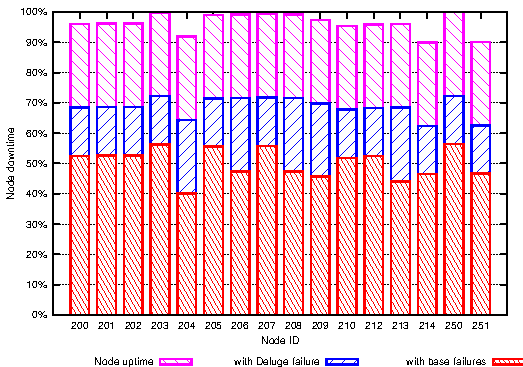
\includegraphics[width=\hsize]{./5-evaluation/figs/robustness/nodesalive/node-uptime2.pdf}
\end{center}
\caption{\textbf{Individual node uptimes.}
This figure shows the percentage of time that each node reported status
messages during the 19-day deployment.  Shown separately are the apparent
node uptimes caused by the whole-network outage and base station outages.
While the former was true sensor node failure, the latter did not seem to
affect the sensor nodes themselves.}
\end{figure}

Figure~\ref{evaluation-fig-nodeuptime} shows the uptime for each node during
the 19-day deployment. Each bar consists of three portions. The lowest
portion is the {\em apparent} uptime of each node accounting for both the
base station failures and single 3-day~software outage. Because base station
failures did not affect individual nodes, the middle bar shows the apparent
uptime including only the 3-day~outage. In this case, the mean node uptime
is~69\%.  However, with the 3-day outage factored out, nodes achieved an
average uptime of~96\%.  These numbers are encouraging and suggest that the
sensor nodes were very reliable in spite of the software crash.

Based on discussions with the authors of Deluge, we believe this failure was
caused by a single bug in the {\tt InternalFlash} TinyOS component (which has
since been fixed).  This bug prevented Deluge from storing critical state
information, causing nodes to reboot continuously at short intervals.  We did
not see this behavior in the lab before deployment, although we had not
rigorously tested this portion of the code. In retrospect, it was optimistic
of us to rely on a complex network reboot protocol that had not been
field-tested.  Deluge was removed from the binary used during the network
reprogram following the failure; it was replaced with a simpler mechanism to
reboot individual nodes using a radio command.

%  - Node reboots [KL]
%    - Determine manual vs. automatic reboots
%    - Correlate reboots to other node properties (routing load?)
%    - Impact of reboot (latency)
%\begin{figure}[t]
%  \begin{center}
%    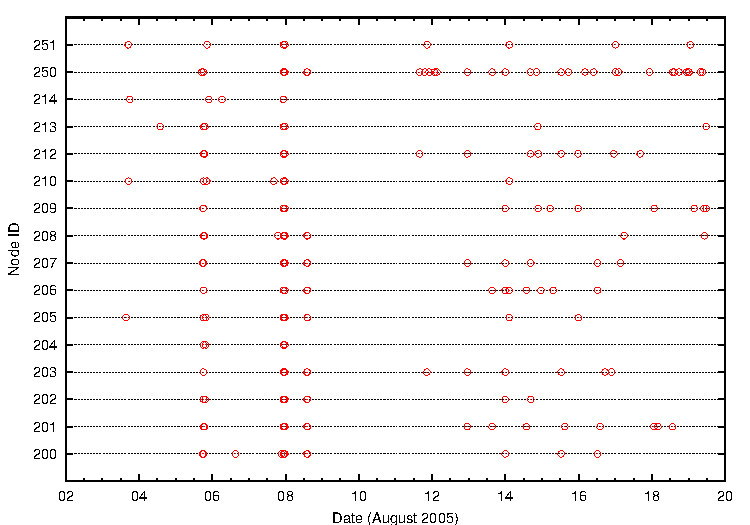
\includegraphics[width=\hsize]{./5-evaluation/figs/robustness/nodeReboots/nodeReboots.pdf}
%  \end{center}
%  \caption{\small{\bf Reboots of each node}
%    {\em This figure shows when each node rebooted during the 19-day deployment.}}
%    \label{fig-nodeReboots}
%\end{figure}


%\begin{figure}[t]
%  \begin{center}
%    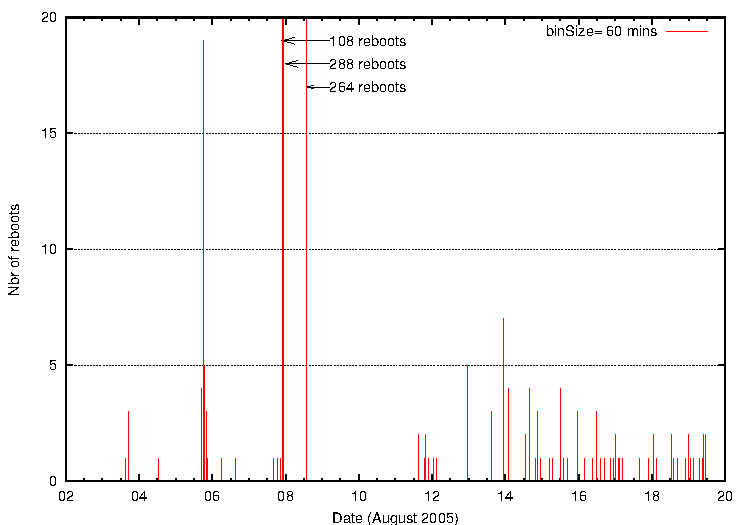
\includegraphics[width=\hsize]{./5-evaluation/figs/robustness/nodeReboots/nodeRebootsBinned.pdf}
%  \end{center}
%  \caption{\small{\bf Number of reboots over time}
%    {\em This figure shows a the number of reboots in 60 minute
%    windows.  As we can see, there was an unusually large number of
%    reboots right before the network reprogramming.}}
%    \label{fig-nodeRebootsBinned}
%\end{figure}

\subsection{Discussion}

Failures of the base station infrastructure were a significant source of
network downtime during the deployment.  This contrasts with common
assumptions that the base station is generally reliable and operating on a
continuous power source. This was our expectation prior to the deployment,
and we did not make adequate preparations for the intermittent electrical
supply at the observatory. A backup diesel generator was used during nightly
power outages, with extra laptop and car batteries supplying power when it
failed.  However, this approach was not ultimately successful.

It may be surprising that node uptime is not related to depth in the routing
tree. This suggests that if a node is ``down'' (i.e., we do not receive any
status messages from it during a 10-minute window) that it is still active
and routing packets for its children in the tree, even as its own status
messages are being lost. An alternate explanation is that a node could select
an alternate parent in the routing topology when its parent fails. However,
our analysis of the routing topology does not support this view, since nodes
rarely use more than one parent. For example, node~214 \textit{always} routes
data through node~251. The volcano-induced failure of node~204 near the end
of the deployment is the only notable failure of a single node.


\section{Event Detector Accuracy}
\label{evaluation-sec-eventdetection}

Our network was designed to capture interesting volcanic signals.  Thus, it
is critical that the system correctly identify and report such events.  This
section evaluates our event detection algorithm both in terms of the number
and rate of event triggers as well as its ability to detect scientifically
interesting events.

\subsection{Event triggers per node}

\begin{figure}[t]
\label{evaluation-fig-eventspernode}
\begin{center}
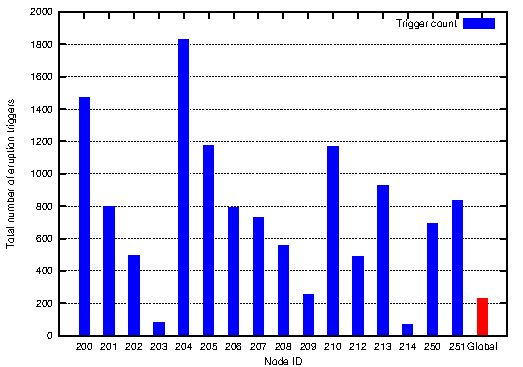
\includegraphics[width=\hsize]{./5-evaluation/figs/eventdetection/eruptionTriggers/eruptCount.pdf}
\end{center}
\caption{\textbf{Event triggers per node.}
This figure shows the total number of event triggers reported by each node.
It demonstrates a wide variation in trigger rates that cannot be attributed
only to varying node uptimes. For example, node~204 had the lowest uptime but
the largest number of event triggers.}
\end{figure}

\begin{figure}[t]
\label{evaluation-fig-eventspertime}
\begin{center}
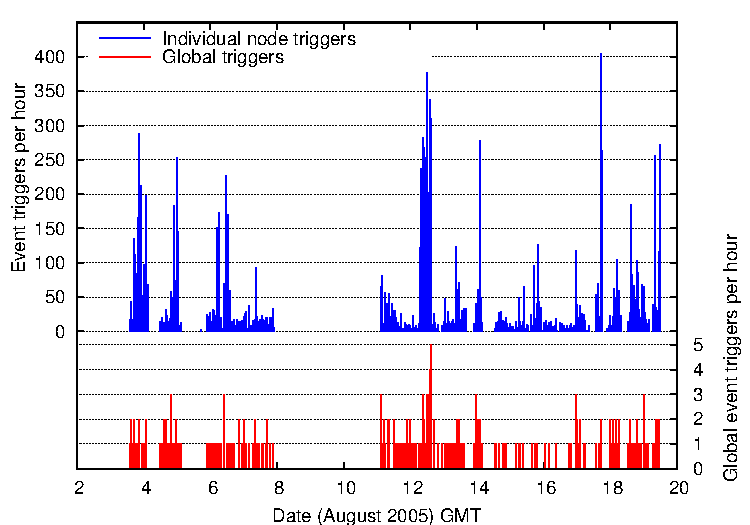
\includegraphics[width=\hsize]{./5-evaluation/figs/eventdetection/eruptionTriggers/eruptCountVsTime.pdf}
\end{center}
\caption{\textbf{Event triggers over time.}
The upper graph shows the total number of individual node triggers per hour.
The lower graph shows the corresponding number of global triggers.
Reventador's varying seismic activity generated between 0~to~5 global
triggers per hour.}
\end{figure}

Figure~\ref{evaluation-fig-eventspernode} shows the total number of events
reported by each node during the deployment. It shows a wide variation in the
event trigger rate, from 70~triggers for node~213 to 1830~triggers for
node~204.  Variation in the trigger rate can be attributed to many factors,
including the location of the node, the orientation of the seismometer, and
the quality of the seismometer-to-ground coupling.  Note that the trigger
rate does not seem to be related to distance from the vent. Although node~204
was closest to the vent and reported the most triggers, nodes 200, 205, and
210 all had high trigger counts despite being significantly farther away.

\subsection{Event triggers over time}

Figure~\ref{evaluation-fig-eventspertime} shows both the number of individual
node and global event triggers over each hour. We observe that the volcano's
activity varied greatly, generating trigger counts ranging between~2~and~405
events per hour when the network was online.  This activity translates into
up to 5~global event triggers an hour, each initiating a Fetch download cycle
of the associated data.

The volcano's bursty and unpredictable activity makes the network's design
more challenging than systems designed for statically-scheduled data
collection.  The data collection protocol, based on our earlier deployment at
Tungurahua~\cite{volcano-ewsn05}, assumed that events would be rare and that
it would be unnecessary to simultaneously record signals for one event while
downloading another. As a result, we missed a number of impressive
back-to-back eruptions typical of the activity at Reventador. It is worth
noting that the variable number of event reports is itself a measure of the
volcano's activity level and could be used to assess hazard levels. 

\subsection{Event detector accuracy}
\label{sec-eventdetectaccuracy}

%  - Event detector accuracy vs. Reftek data [MDW]
%    - Vary E.D. parameters

The network detected 229~eruptions, explosions, earthquakes, and tremor
events during the deployment. Ideally, we would like to assess its accuracy
in terms of the fraction of true events detected, as well as the false
positive rate. Given the high degree of coherence required by the global
event detector (requiring 30\% of the active nodes to trigger within a short
time window), we would be surprised if the sensor network recorded any false
events. Indeed, all of the signals we did capture appear to be based on true
volcanic activity, indicating a zero false positive rate.

We intended to apply our event detection algorithm to the signals collected
by the two broadband seismic stations to establish the algorithm's accuracy.
Unfortunately, we found this to be difficult for several reasons.  First,
each of the broadband stations suffered intermittent power and software
failures, either preventing them from logging any data, or corrupting the
collected signals or timestamps.  Thus, even in those cases where broadband
data is available, it is not always accurate. 
%Moreover, intermittent noise on a single broadband station could be
%interpreted as an event by our algorithm, yielding an artificially high
%trigger rate. 
Second, the broadband stations deployed a more sensitive seismometer with a
much wider frequency response.  The geophones used by our sensor nodes have a
corner frequency of 4.5~Hz, while the broadband sensors have a corner
frequency of 0.033~Hz.  Additionally, the broadband seismometers are much
more sensitive, generating voltages of 800~V/m/sec, whereas the geophones
have a sensitivity of only 32~V/m/sec. As a result, the broadband sensors are
able to detect much weaker seismic signals.

We focus our attention on a single day of data where the broadband stations
were recording clean data and the sensor network was relatively stable. One
of the authors, a seismologist, visually extracted events from the broadband
data; during this 24-hour period, a total of 589~events were recorded by the
broadband sensors. During the same time, the sensor network triggered on just
7~events, suggesting that our detection accuracy is very low (about 1\%).

The network could have failed to detect a seismic event for one of four
reasons: (1) failure of individual nodes; (2) failure of the base station or
radio modem; (3) the low sensitivity of our seismometers; or (4) failure of
the event detection algorithm itself. To factor out the increased sensitivity
of the broadband seismometers, we only consider the 174~events with SNR~$\geq
10$ from both stations, which we expect the geophones should have been able
to detect as well.  Also, Section~\ref{evaluation-sec-robustness} has already
addressed the question of uptime, so we focus here on the inherent accuracy
of the event detector when the network was operating correctly. 136~of the
174~broadband events occurred during times when the network was operational.
Taking these two factors into account, the network's detection accuracy is
still only about 5\%. 

%It is not
%clear how to tune the event detection algorithm for the broadband data.
%If the algorithm is not sensitive enough, it will fail to detect events that
%our network did in fact report.  If the algorithm is too sensitive, it will
%report false events that the sensor network should not have reported. 
%Although our EWMA-based algorithm was developed after consultation
%with seismologists, there is no single gold standard for event detection in
%the volcanological community.
%However, we did not experiment with different event-detection parameters in
%the field, as the number of eruptions and earthquakes triggering the current
%detector was more than adequate to exercise the network.  For our deployment
%the sheer volume of data precludes manual selection of events.

%In an attempt to assess the event detector's accuracy, we
%applied our original event-detection algorithm to the filtered 
%broadband data from August~11--19, which corresponds to 143~events 
%captured by our sensor network. 75~out of these~143 events (52\%) 
%have a trigger from at least one broadband station; 47~events (32\%)
%have triggers from both stations. The lack of triggers for the 
%remaining events (all of which are true seismic activity) 
%is due to corruption or gaps in the broadband data. 

%143~events from August 11--19 which were properly time rectified as described
%in Section~\ref{sec-timing}.  Of these events, 142 had corresponding data
%from at least one broadband station.  We then ran the original event
%detection algorithm on the broadband signals.
%%In addition, we lowered the EWMA ratio threshold of the detector from 1050
%%to 1030, making the detector much more sensitive than the mote detector.
%Due to the small number of broadband stations we consider a trigger from 
%{\em either} station as identifying a meaningful event. This implies that
%noise on a single station can increase our false positive rate.

% PARAMETERS USED HERE:
%   - Broadband event detector: low gain 1.0, high gain 9.0, threshold 1050
%   - Vote count required: 1 
%   - No suppression
%This resulted in 12505~individual triggers from the broadband data.
%123~out of the~142~events (87\%) had a
%corresponding trigger in the broadband data.  
%Given the high degree of
%coherence required by the global event detector (requiring 5~nodes to
%trigger within a short time window), we would be surprised if the sensor
%network recorded any spurious events. Indeed, all of the signals we did
%capture appear to be based on true volcanic activity.  
%We suspect that the
%lack of triggers for the remaining 19~events is due to corruption in the
%broadband data.
%However, with only 3~broadband stations, any one of
%which could have been faulty at any time, it is difficult to use this
%data to definitively evaluate event detection accuracy. 

%%%%%%%%%%%%%%%%%%%%%%%%%%%%%%%%%%%%%%%%%%%%%%%%%%%%%%%%%%%%%%%%%%%%%%%%%%%%
%%% MDW: Original text here:
%The more difficult question is what fraction of ``true'' events were
%successfully detected. As discussed above, without a gold standard for event
%detection and complete broadband data coverage, it is impossible to make 
%a direct comparison. The best we can do is use our original 
%event-detection algorithm on the broadband data and compare the 
%set of triggers to those reported by our network.
%
%Using the same global detector parameters (requiring both broadband
%stations to trigger within a 10~sec window) 
%yields 285 events in the broadband data set.
%%(a significant reduction from the 12505 individual triggers, suggesting very
%%high noise in the broadband data).
%Of these, 36 events (13\%) correspond to events recorded by our network.
%Each of remaining 249 missing events is the result of either the failure of
%the event detector, the failure of the sensor network, or false positives
%in the broadband data set. With only two broadband stations it is
%difficult to tease these reasons apart.  Of the 136 broadband events that
%occurred while all 16~nodes of the sensor network were operational, our
%network detected~24. If the broadband stations are considered ground truth
%this results in a detection accuracy of 17.7\%. 
%%%%%%%%%%%%%%%%%%%%%%%%%%%%%%%%%%%%%%%%%%%%%%%%%%%%%%%%%%%%%%%%%%%%%%%%%%%%

%%%%%%%%%%%%%%%%%%%%%%%%%%%%%%%%%%%%%%%%%%%%%%%%%%%%%%%%%%%%%%%%%%%%%%%%%%%%
%%% MDW: New text here:

%Without complete broadband data coverage, there is no way to tell how
%many true events occurred.  For sake of argument, let us consider the set
%of seismic events triggered in {\em both} broadband stations, a total
%of 406~triggers, as ``ground truth.''  However, because there are only
%two broadband stations, we expect a high false positive rate in the
%broadband data.  For example, if we had required only two~sensor votes 
%to trigger (rather than five), the number of sensor node events jumps 
%from 70~to~462 (an increase of 660\%) suggesting that the broadband
%trigger rate is artificially high.

%To compare the sensor network and broadband triggers, 
%We dilate each broadband trigger by 60~sec and consider
%any sensor network trigger that falls within this window to be 
%a match. 27~out of~the~70~(38\%) sensor network triggers match some 
%broadband trigger. Combining the broadband and sensor network
%triggers, there are 449~unique events; the sensor network detected 6\%. 
%However, it is worth noting
%that the broadband station missed 43~of the 70~sensor network events,
%likely due to missing data. The fact that the
%sensor network and broadband triggers are poorly correlated
%suggests that using the broadband stations is not an accurate 
%measure of ground truth. 

Recall that during a Fetch download cycle, nodes disabled sampling to avoid
overwriting data in flash. Download cycles could take up to several minutes
{\em per node} (see Section~\ref{evaluation-sec-performance}), meaning that
there are significant time windows when the network was unable to detect new
events.  During the Fetch cycles on August 15, the broadband stations
recorded 42~events, 24\% of the total events detected.  This indicates that,
all else being equal, the sensor network could have detected approximately
24\% more events had we designed the protocol to sample and download
simultaneously. We plan to add this feature in the next version of our
system.

In the end, we believe that our low detection rate is the result of the
parameters used in the EWMA-based event detection algorithm.  These
parameters were chosen prior to the deployment, based on our experience with
detecting infrasonic events at a different volcano~\cite{volcano-ewsn05}. We
did not experiment with modifying them in the field. Indeed, using our
algorithm with these same parameters on the broadband data for August~15
detects only 101~events, a fraction of the events chosen manually by an
expert.  We plan to tune our event-detection parameters for future
deployments based on the data collected by the broadband stations.

%Because we cannot define ground truth in absolute terms, we cannot
%directly report on the specificity and sensitivity of our event detection
%algorithm. Instead, we verify that for each event recorded by the
%sensor network, the same event-detection algorithm applied to the
%corresponding broadband station data would have also reported an 
%event. This is a measure of how many ``false positives'' are reported
%by the sensor network but does not capture ``false negatives.''
%
%We took a representative set of 78~events that appear to have accurate 
%timing (as described in Section~\ref{sec-timing}). We then applied our
%original event-detection algorithm on the corresponding data from 
%the RRVEN and RHOTEL stations (eliding station RLAV3 for the reasons 
%described above). The same event-detection parameters were used as
%by the motes in the original deployment. As expected, the algorithm 
%applied to the broadband data triggered events in 100\% of these cases, 
%meaning that there are no false positive events in our data set.

%less consensus about what constitutes a ``real event.''
%It is an open question what proportion of ``true'' events we
%successfully captured. 

%Applying our
%original algorithm to the broadband data set for August 11--19 
%reports 315~unique events. During the same period the sensor network
%reported 144~events. Only 33 events, or 23\% of the events reported
%by the network, match in both data sets. This is due to many factors.

%\begin{figure*}[t]
%\begin{tabular}{|llllll|} \hline
%{\bf Suppression window} & 
%{\bf Broadband events} &
%{\bf Mote events} &
%{\bf Matching events} & 
%{\bf ``False positive'' \%} & 
%{\bf ``False negative'' \%} \\ \hline
%{\bf 1 votes needed, thresh 1050} & & & & & \\ \hline
% {\em none}	& 8031 & 144 & 89 & 38\% & 99\% \\  \hline
%{\bf 2 votes needed, thresh 1050} & & & & & \\ \hline
% {\em none}	& 3530 & 144 & 37 & 74\% & 99\% \\  \hline
%\end{tabular}
%\caption{\small \XXXnote{finish this!}}
%\end{figure*}
%
%  - Global detector accuracy [MDW]
%    - How well did global detector filter out false events
%    - Specificity/sensitivity analysis [MDW - hold off]



\section{Data Collection Performance}
\label{evaluation-sec-performance}

In this section we assess the performance of the {\em Fetch} data collection
protocol. We evaluate Fetch in terms of its {\em yield}, its ability to
successfully collect requested data; and its {\em latency}, the time to
download events from the network.

\subsection{Data yield}

We define the {\em event yield} of a Fetch transfer as the fraction of nodes
for which the entire 60~sec signal was successfully downloaded following an
event. The calculation only considers those nodes that were active at the
time of the event detection (Figure~\ref{evaluation-fig-nodesalive}).  For
example, if 10~nodes were active during an event, then the event yield is
defined in terms of 10~nodes.  Note that the Fetch protocol attempts to
download a signal from all active nodes, even those that did not detect the
event.

\begin{figure}[t]
\label{evaluation-fig-compBlockYieldCDF}
\begin{center}
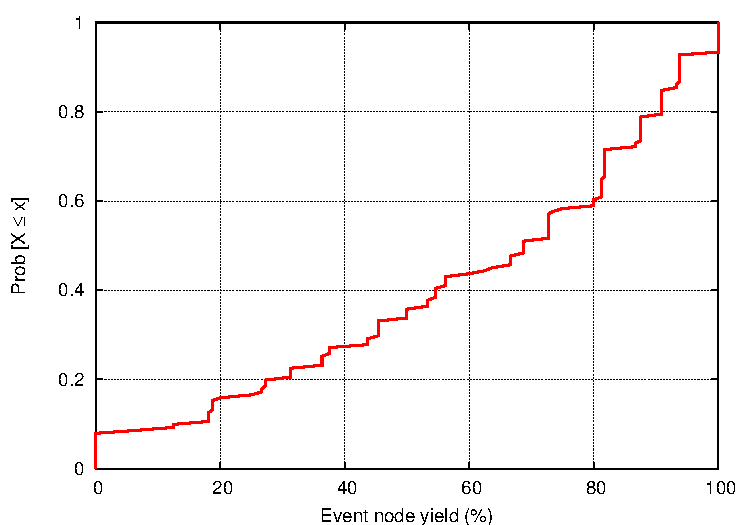
\includegraphics[width=\hsize]{./5-evaluation/figs/performance/yields/comparison/availableEventNodeYieldCDF.pdf}
\end{center}
\caption{\textbf{vent yield.}
This graph shows a CDF of the event yield for each of the 229~events recorded
during the entire deployment. Event yield is the fraction of active nodes
from which a complete 60~sec signal was downloaded following an event.}
\end{figure}

Figure~\ref{evaluation-fig-compBlockYieldCDF} shows a CDF of the event yield
for all 229~events recorded during the deployment.  As the figure shows, the
median event yield was 68.5\% and the 90th percentile was 94\%.  The yield
can be affected by several factors.  First, the protocol will abort a
transfer from a node after re-requesting the same block more than 20~times,
or if the transfer from a single node exceeds 10~minutes.  Second, because
sampling is disabled while performing a data transfer, if two back-to-back
events occur a node may not end up storing data for the second event.


% ------ Original text ------------------------
%% In this section we assess the performance of the {\em Fetch} data collection
%% protocol. We evaluate Fetch in terms of its {\em yield}, its ability 
%% to successfully collect requested data; and its {\em latency}, the 
%% time it took to download events from the network.

%% \subsection{Data yield}
%% %  - Yield [KL]
%% %    - % of detected events that we successfully downloaded data for
%% %    - How much data per event
%% %    - Consider all nodes vs. only "active" nodes
%% %    - Before and after reprogram

%% We define the {\em event block yield} of a Fetch transfer as the fraction of
%% requested data blocks successfully downloaded from each node following an
%% event. The calculation only considers those nodes that were operational at
%% the time of the event detection. For example, if 10~nodes were active during an
%% event, then the event block yield is defined as the fraction of data blocks
%% retrieved from those 10~nodes.  Normally, following an event the system would
%% attempt to download 60~sec of data from each operational node, including
%% nodes that did not report the event. 

%% \begin{figure}[t]
%% \begin{center}
%% 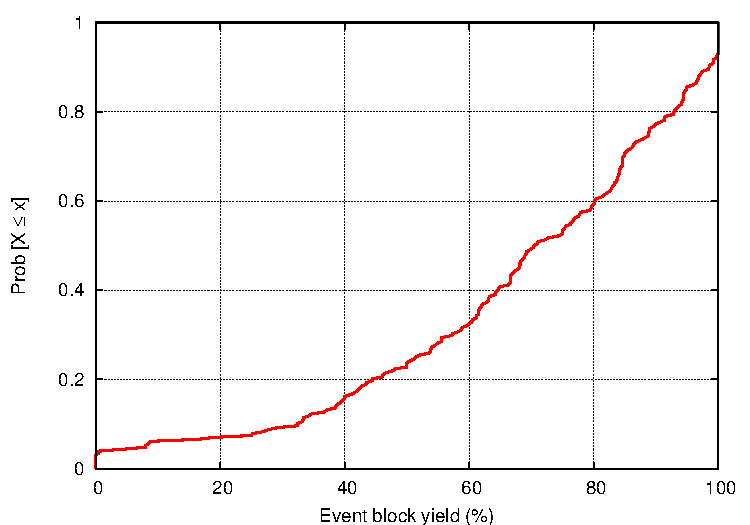
\includegraphics[width=\hsize]{./5-evaluation/figs/performance/yields/comparison/schBlockYieldCDF_entire.pdf}
%% \end{center}
%% \caption{\small{\bf Event block yield.}
%% {\em This graph shows a CDF of the event block yield for each of the 229~events
%% recorded during the entire deployment.}}
%% \label{fig-compBlockYieldCDF}
%% \end{figure}

%% Figure~\ref{fig-compBlockYieldCDF} shows a CDF of the event block
%% yield for all 229~events recorded during the deployment.  As the
%% figure shows, the median event block yield was 70.4\% and the 90th
%% percentile was 98.6\%.  The yield can be affected by several factors.
%% First, the protocol will abort a transfer from a node after
%% re-requesting the same block more than 20~times, or if the transfer
%% from a single node exceeds 10~minutes.  Second, because sampling is
%% disabled while performing a data transfer, if two back-to-back events
%% occur a node may not end up storing data for the second event.
% --------------------------------------------------------


%The event block yield of each transfer is affected by several factors.
%First, the Fetch protocol will timeout on a transfer from a node after
%re-requesting the same block more than 20~times, or if the cumulative
%transfer time from a single node exceeds 10~minutes.	Second, the protocol
%may request blocks not in a node's cache.  Because we disable sampling during
%a Fetch transfer, if two back-to-back events occur the second Fetch operation
%may attempt to request blocks that the node never stored because it was busy
%with the first transfer. Or we may simply fail to disable sampling on a
%particular node causing the requested blocks to be overwritten before we are
%able to retrieve them. 

%Also shown is a breakdown of the
%event block yield both before and after the network was reprogrammed on
%August 11, 2005 following the Deluge failure. After the
%reprogramming, the median event block yield improved from 66.7\% to 77.8\%. 

%The improvement is due to several changes that were introduced
%following the reprogramming in an attempt to improve the performance
%and robustness of the Fetch protocol based on our observations in the
%first few days of the deployment.  First, the transfer timeout was
%increased from 10~minutes to 20~minutes, giving nodes more time to
%respond to Fetch requests. Second, the speed at which Fetch commands
%were propagated through the network was increased by a factor of~4,
%decreasing the latency for a Fetch request to reach a node.  Third, we
%disabled duplicate suppression in the flooding protocol used to
%propagate Fetch requests to the network, increasing overall network
%load but increasing reliability.

%Figure~\ref{fig-compNodePercentiles} shows the 50th-percentile yield
%for each node before and after network reprogramming.  The yield for
%most nodes is very good (100\% in most cases), with a couple of
%exceptions.  In general, the yield is highest for nodes that were
%closest to the root of the tree and for those that only had 2
%channels.  This is consistent with our expectations.  When the base
%station concludes that there was an event, it first floods the network
%with a command telling nodes to stop sampling.  Afterwards, it
%downloads the event data from each node in a round-robin fashion,
%ordered by hop count from the root.  We observed that the stop
%sampling message did not always propagate to all the nodes, with nodes
%farter away from the root beeing less likely to have received the stop
%sampling command.  If a node did not stop sampling, there was a good
%chance that it might have overwritten it's circular flash buffer by
%the time it was scheduled to be downloaded.  Again this is more likely
%for nodes farter away because they were scheduled later.  The two
%nodes with 4 channeles, 250 and 251, produce twice as much data than
%the 2-channel nodes and therefore fill in their falsh at twice the
%rate.  Note that node 251 was also the second farthes node from the
%root after node 214.
%
%In Figure~\ref{fig-compNodePercentiles} we also see that after the
%network reprogramming, the yield for each node improved or stayed the
%same.  \XXXnote{add explanations}.

%\begin{figure}[t]
%\begin{center}
%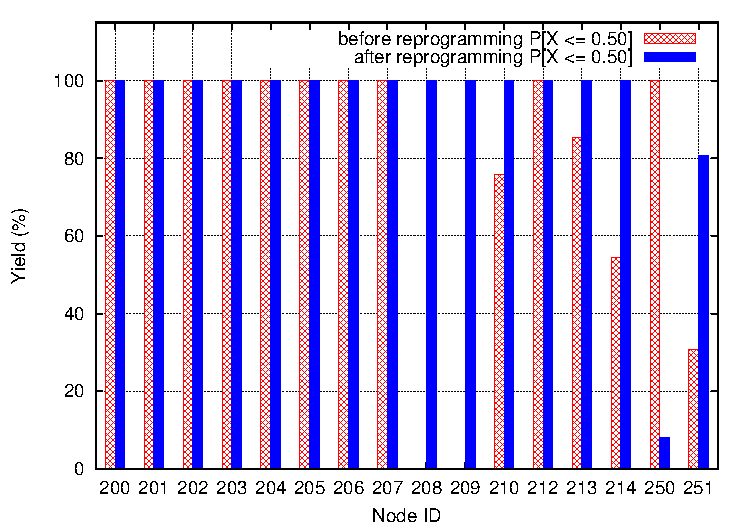
\includegraphics[width=\hsize]{./5-evaluation/figs/performance/yields/comparison/nodePercentiles.pdf}
%\end{center}
%\caption{\small{\bf 50th-percentile yield by nodeID before and after network reprogramming.}
%{\em The 50th-percentile yield for most of the nodes is very good,
%with a few exceptions.  After the network reprogramming, the yield for
%all nodes either improved or stayed the same.}}
%\label{fig-compNodePercentiles}
%\end{figure}

%% \XXXnote{MDW: The previous definition of ``node yield'' did not make
%% sense to me. I have tried to reword this but Konrad needs to check
%% that this is right. It does not make sense to ``download a node.''}

Next, we look at the {\em node yield} which we define as the probability that
an event was successfully downloaded from a given node.  Like the event
yield, the calculation only considers those nodes that were active at the
time of each event detection.  Node yield can be affected by several factors.
The depth and radio link quality of a node's routing path to the base station
affect packet loss rate and thereby the likelihood of a Fetch timeout.
%The farther a node is from the root of the tree, and the more low-quality
%links it has to route across, the more likely its packets will get lost.  
Additionally, two nodes outfitted with triaxial seismometers
(nodes~250~and~251) sample and store twice as much data as the others,
increasing the probability of a timeout.  Finally, a bug in our control
application caused node~250 to sample data continuously, even during a Fetch
operation. As a result, this node was more likely to overwrite an event
stored in flash before it could be downloaded.

\begin{figure}[t]
\label{evaluation-fig-nodeYield}
\begin{center}
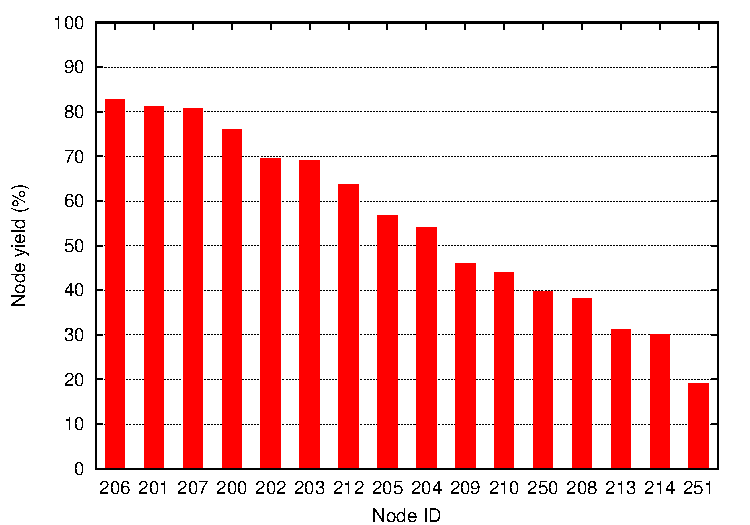
\includegraphics[width=\hsize]{./5-evaluation/figs/performance/yields/nodeYield/nodeYieldOnly.pdf}
\end{center}
\caption{\textbf{Node yield.}
This graph shows the node yield for each of the 16 nodes over the entire
deployment, defined as the probability that an event was successfully
downloaded from a node, as long as that node is active during the
corresponding event detection.}
\end{figure}

%% \XXXnote{MDW: I am very confused by this figure and the terminology
%% here. What does ``the total number of times a node was available and
%% successfully downloaded'' mean? I think we should probably just
%% eliminate the extra bars from the figure here, and only show the node
%% yield by itself. We have already shown the node uptimes in another figure.}

Figure~\ref{evaluation-fig-nodeYield} shows the node yield for each of the
nodes.
%% For comparison, it also shows the total number of times a node was
%% available and successfully downloaded for the entire deployment.  
We can see how the factors mentioned above affected performance.  First, the
nodes with the highest yield (above 80\%) tend to be within two hops from the
root (see Figure~\ref{evaluation-fig-schematic}).  However, despite being
within two or three hops, node~209 had a fairly low yield.  This is explained
by the fact that node~209 had a poor link to its closest parent, node~200.
In fact, although most nodes had a stable parent throughout the deployment,
node~209 used node~200 as its parent only 33\% of the time and nodes
206~and~207 the remaining 66\% of the time.  Node~213 also switched parents
between nodes 204~and~208, but unlike node~209 it was always three hops away.
Node~214 was the farthest node in terms of hopcount and as a result had one
of the lowest yields.  The larger amount of data was also a factor for the
four-channel nodes, 250~and~251. In addition, node~251 was five radio hops
from the gateway.


% -------- Original text ---------------------------------------------
%% Next, we look at the {\em node block yield} which we define as the fraction
%% of requested data blocks successfully downloaded from each node.
%% The node block yield can be affected by several 
%% factors. The depth and radio link quality of a node's routing path 
%% to the base station affect packet loss rate and thereby the likelihood
%% of a Fetch timeout.
%% %The farther a node
%% %is from the root of the tree, 
%% %and the more low-quality links it has to route
%% %across, 
%% %the more likely its packets will get lost.  
%% Additionally, two nodes outfitted with triaxial seismometers
%% (nodes~250~and~251) sample and store twice as much data as the others,
%% increasing the likelihood of failure.  Finally, a bug in our control
%% application caused node 250 to sample data continuously, even during a Fetch
%% operation. As a result, this node was more likely to overwrite an 
%% event stored in flash before it could be downloaded.

%% \begin{figure}[t]
%% \begin{center}
%% 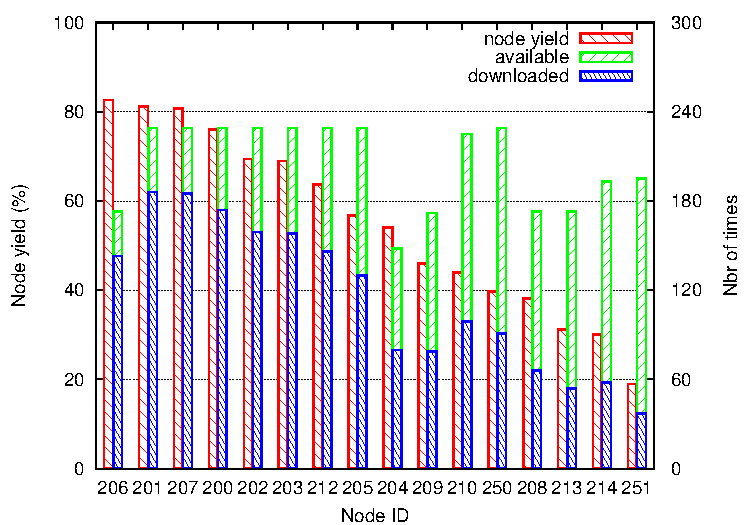
\includegraphics[width=\hsize]{./5-evaluation/figs/performance/yields/nodeYield/nodeYield.pdf}
%% \end{center}
%% \caption{\small{\bf Node block yield.}
%% {\em This graph shows the node block yield for each of the 16 nodes
%%   over the entire deployment. For comparison, the graph also shows the
%% total number of scheduled and downloaded blocks for each node on the 
%% right-hand $y$-axis.}}
%% \label{fig-nodeYield}
%% \end{figure}

%% Figure~\ref{fig-nodeYield} shows the node block yield for each of the nodes.
%% For comparison, it also shows the total number of blocks scheduled and
%% downloaded for the entire deployment.  We can see how the factors mentioned
%% above affected performance.  First, the blocks with the highest yield (above
%% 85\%) tend to be within two hops from the root (see
%% Figure~\ref{fig-schematic}).  However, despite being within two or three hops
%% node~209 had one of the lowest yields.  This is explained by the fact that
%% node~209 had a poor link to its closest parent, node~200.  In fact, although
%% most nodes had a stable parent throughout the deployment, node~209 used 
%% node~200 as its parent only 33\% of the time and nodes 206~and~207 
%% the remaining 66\% of the time.  
%% Node~213 also switched parents between nodes 204~and~208, but
%% unlike node~209 it was always three hops away.  Node~214 was the farthest
%% node in terms of hopcount and as a result had one of the lowest yields.  
%% The larger amount of data was also a factor for the four-channel nodes, 
%% 250~and~251. In addition, node~251 was five radio hops from the gateway.
% --------------------------------------------------------------


%% ; node 250 was continousely sampling, and therefore Fetch could not %
%always reach it before it overwrote the relevant data.

%% \begin{figure}[t]
%% \begin{center}
%% 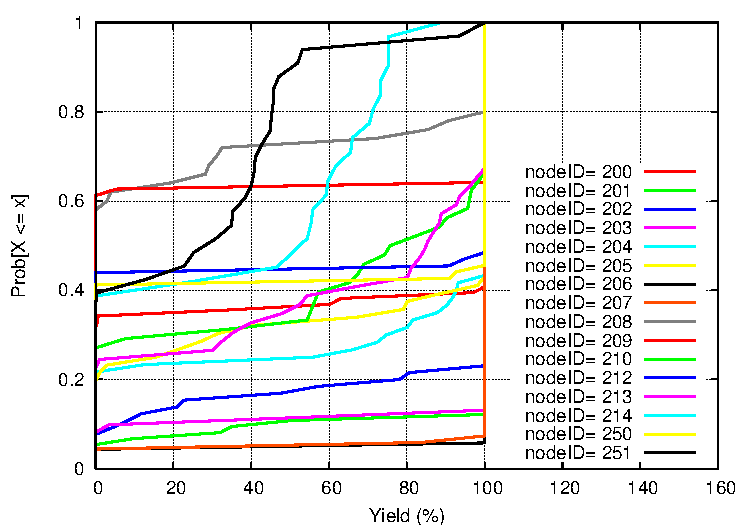
\includegraphics[width=\hsize]{./5-evaluation/figs/performance/yields/beforeReprogram/schBlockYieldCDFByNode.pdf}
%% \end{center}
%% \caption{\small{\bf Block yield by nodeID before network reprogramming.}
%% {\em This graph shows CDFs of the block yields for each node.  The
%% yields for some of the nodes is much higher (mostly the ones that were
%% farther in the routing tree) than for others.}}
%% \label{fig-blockYieldByNodeBeforeReprog}
%% \end{figure}

%% \begin{figure}[t]
%% \begin{center}
%% 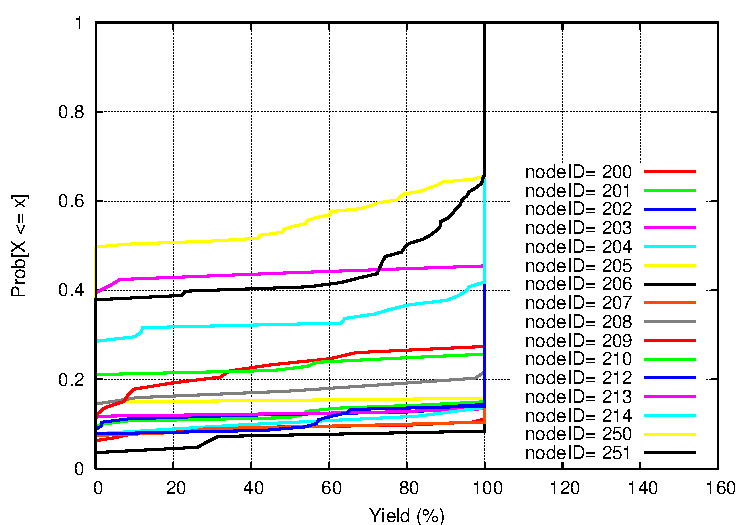
\includegraphics[width=\hsize]{./5-evaluation/figs/performance/yields/afterReprogram/schBlockYieldCDFByNode.pdf}
%% \end{center}
%% \caption{\small{\bf Block yield by nodeID after network reprogramming.}
%% {\em This graph shows CDFs of the block yields for each node.  The
%% yields for some of the nodes is much higher (mostly the ones that were
%% farther in the routing tree) than for others.}}
%% \label{fig-blockYieldByNodeAfterReprog}
%% \end{figure}


%% \begin{figure}[t]
%% \begin{center}
%% 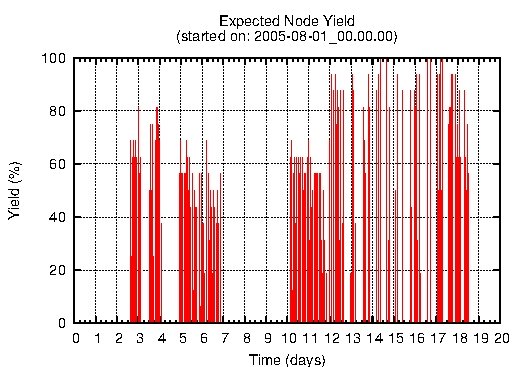
\includegraphics[width=\hsize]{./5-evaluation/figs/performance/yields/expNodeYield.pdf}
%% \end{center}
%% \caption{\small{\bf Expected node yield.}
%% {\em This graph shows the node yield out of the 16 nodes.  Only nodes
%% for which the enitre event was downloaded successfully are considered.}}
%% \label{fig-expNodeYield}
%% \end{figure}

%% \begin{figure}[t]
%% \begin{center}
%% 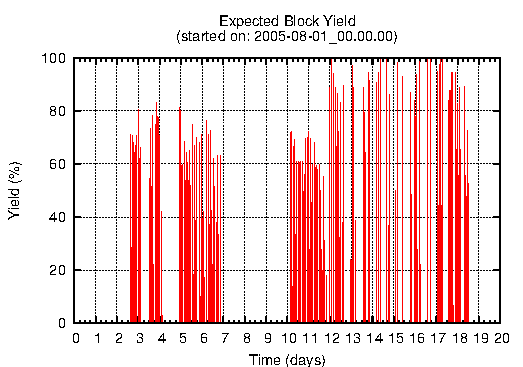
\includegraphics[width=\hsize]{./5-evaluation/figs/performance/yields/expBlockYield.pdf}
%% \end{center}
%% \caption{\small{\bf Expected block yield.}
%% {\em This graph shows the block yield out of the 16 nodes.  Only block
%% for which the enitre block was downloaded successfully are considered.}}
%% \label{fig-expBlockYield}
%% \end{figure}

%% \begin{figure}[t]
%% \begin{center}
%% 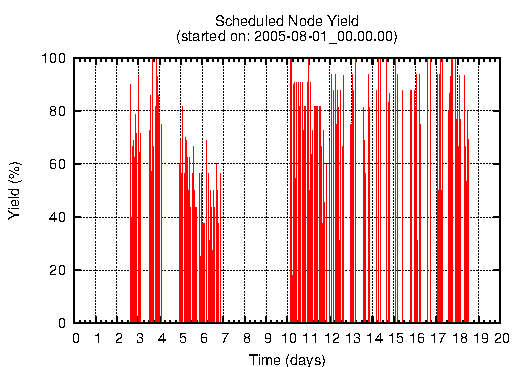
\includegraphics[width=\hsize]{./5-evaluation/figs/performance/yields/schNodeYield.pdf}
%% \end{center}
%% \caption{\small{\bf Scheduled node yield.}
%% {\em This graph shows the node yield out of the scheduled nodes for
%% each event.}}
%% \label{fig-schNodeYield}
%% \end{figure}

%% \begin{figure}[t]
%% \begin{center}
%% 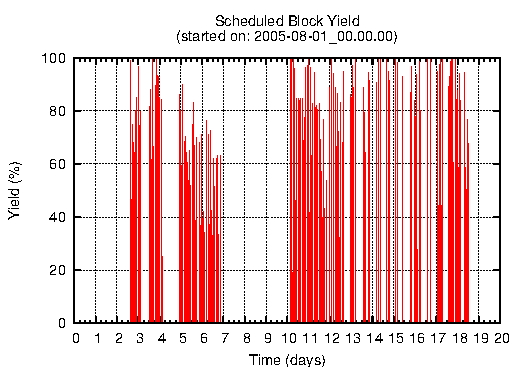
\includegraphics[width=\hsize]{./5-evaluation/figs/performance/yields/schBlockYield.pdf}
%% \end{center}
%% \caption{\small{\bf Scheduled block yield.}
%% {\em This graph shows the block yield out of the scheduled block for
%% each event.}}
%% \label{fig-schBlockYield}
%% \end{figure}

\subsection{Fetch latency}

Transfer latency directly impacts data yield. Because we disabled sampling on
each node (apart from node~250) during a Fetch download cycle, the duration
of the data transfer also affects a node's ability to record back-to-back
events.  

\begin{figure}[t]
\label{evaluation-fig-fetchlatency-byhops}
\begin{center}
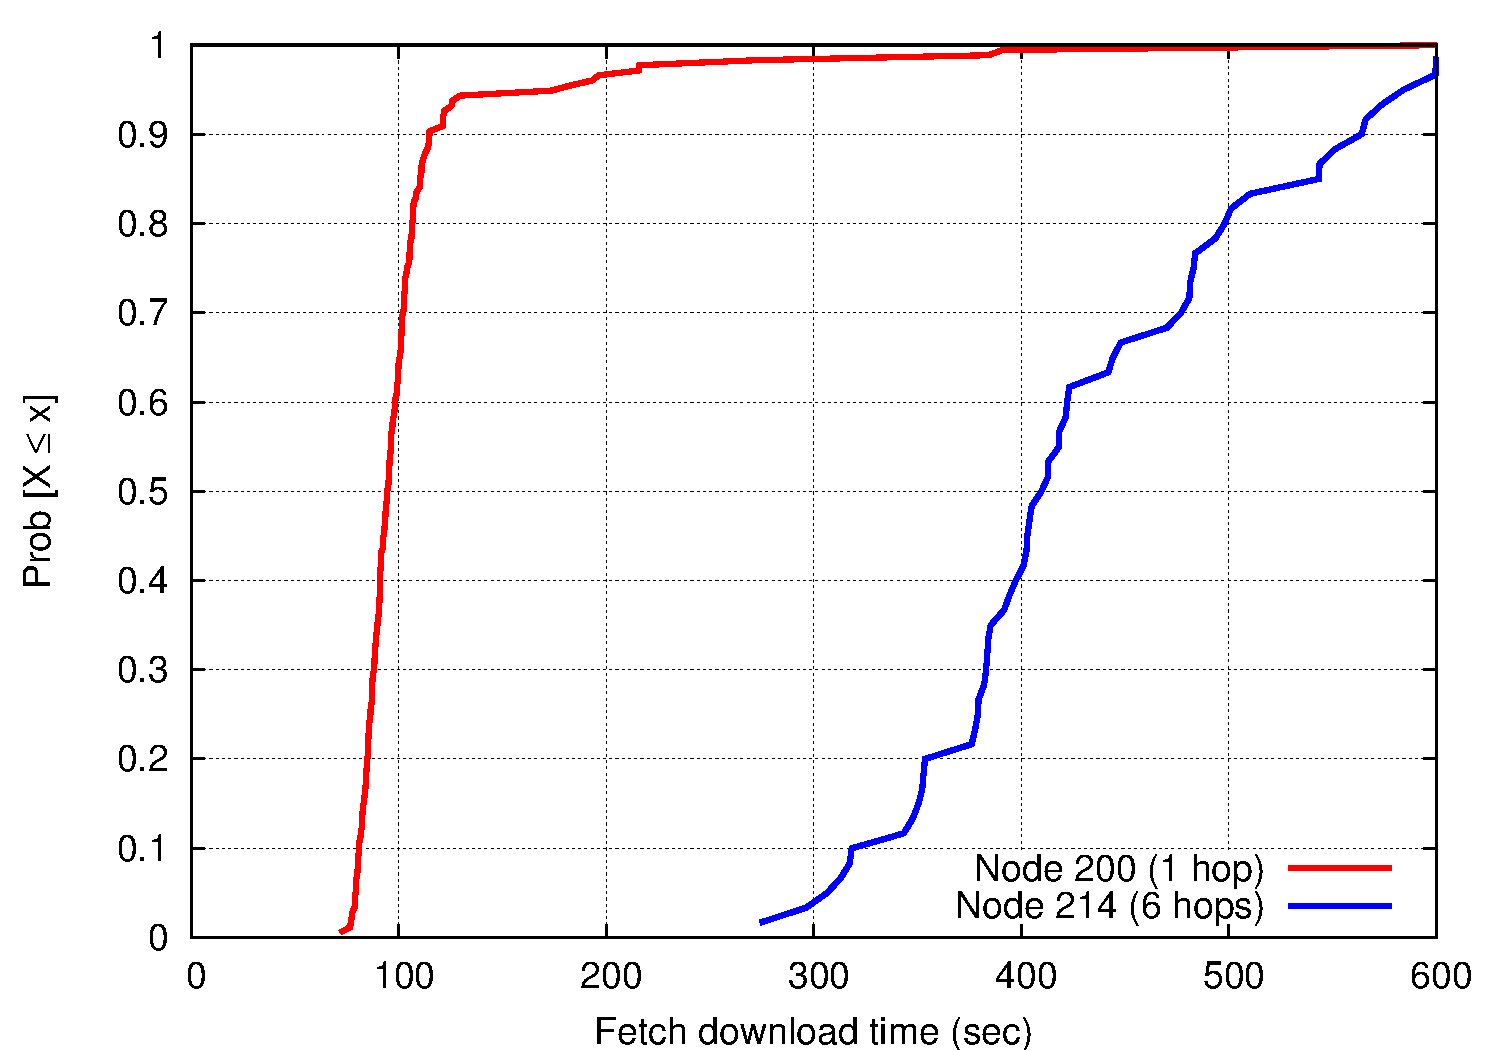
\includegraphics[width=\hsize]{./5-evaluation/figs/performance/CDFByHops/CDFBYHOPS.pdf}
\end{center}
\caption{\textbf{Distribution of Fetch latency for two nodes.}
The latency for a Fetch download depends on the depth of the node in the
routing tree, which affects both command propagation latency and reliability
of the routing path. Node~200 is located 1~hop from the sink and node~214 is
located 6~hops away.}
\end{figure}

The median latency for Fetch operations (downloading 60~sec worth of data
from a single node) was 186~sec and the 90th percentile was 444~sec.
Unsurprisingly, latency varies with the depth of the node in the routing
tree. Figure~\ref{evaluation-fig-fetchlatency-byhops} compares Fetch latency
for nodes 200~and~214, located 1~and~6 hops away from the sink, respectively.
Node~200 had a median Fetch latency of 94~sec, while node 214~had a median
latency of 409~sec, about 63~sec per hop.  This is due to both increased
delay for propagating Fetch command messages, as well as increasing packet
loss and retransmission overheads as the data flows over multiple hops to the
base.

%\begin{figure}[t]
%\begin{center}
%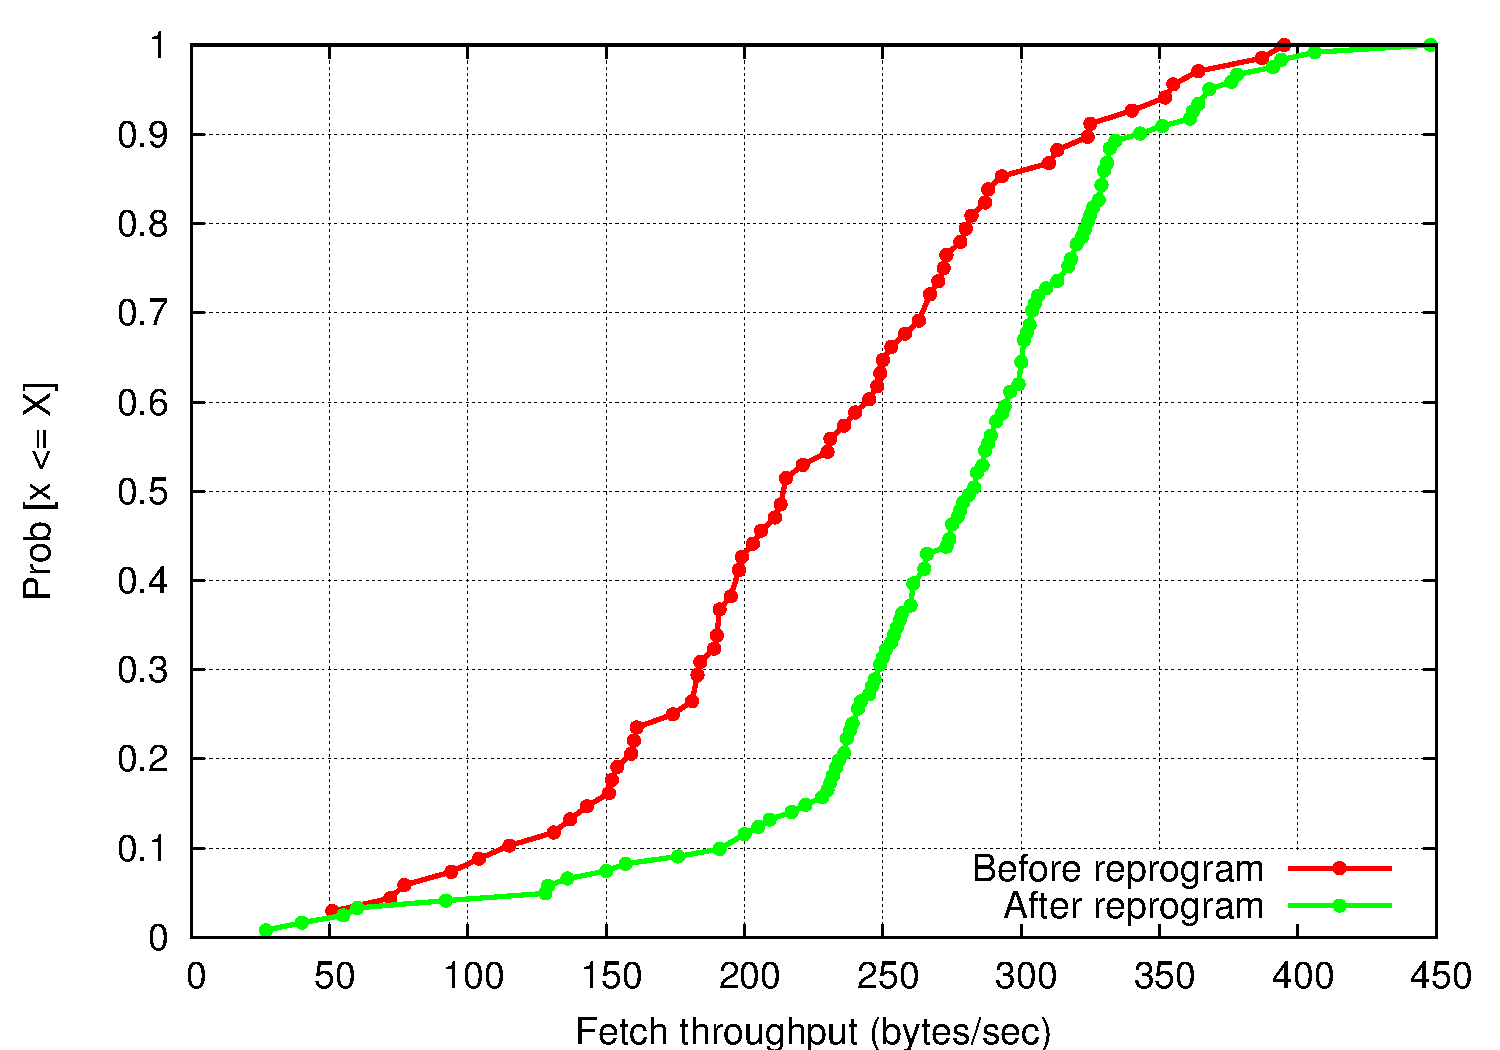
\includegraphics[width=\hsize]{./5-evaluation/figs/performance/fetchspeed/fetchspeed-cdf-oldnew.pdf}
%\end{center}
%\caption{\small{\bf Fetch throughput.}
%{\em This graph shows a CDF of the the throughput for each Fetch
%operation before and after the node reprogram. 
%Before programming, the median throughput was XXX~bytes/sec and after
%the median was~XXX~bytes/sec.}}
%\label{fig-fetchspeed-oldnew}
%\end{figure}

%Figure~\ref{fig-fetchspeed-oldnew} shows a CDF of the throughput of
%each Fetch operation from each node following an event. Before
%the network reprogram on August 11, the median throughput was
%215~bytes/sec; after the reprogram the median increased to 283~bytes/sec.
%While these values are far less than the peak thoughput achievable
%by the radio (which can exceed 12000 bytes/sec when MAC delays
%are accounted for), it is important to note that the Fetch protocol
%was never designed to maximize throughput. In particular, the 
%protocol requests a single block at a time from the network, and
%uses a long delay (up to 1~sec) before retransmitting a block request.

Fetch was initially designed to support reliable downloads of infrequent
events and we did not anticipate the need to capture back-to-back signals.
Unfortunately, these were common at Reventador, and may necessitate a
redesign. For example, it may be possible to reduce latency by streaming
multiple blocks in one request and reconstructing partial blocks after a
burst. Caching recently-received blocks on intermediate nodes could reduce
latency for repair requests~\cite{netshm-emnets05}.  However, such changes
would greatly increase the complexity of the protocol. For this deployment we
opted to prioritize simplicity and stability over performance.

%   - Throughput by hopcount
%\begin{figure}[t]
%\begin{center}
%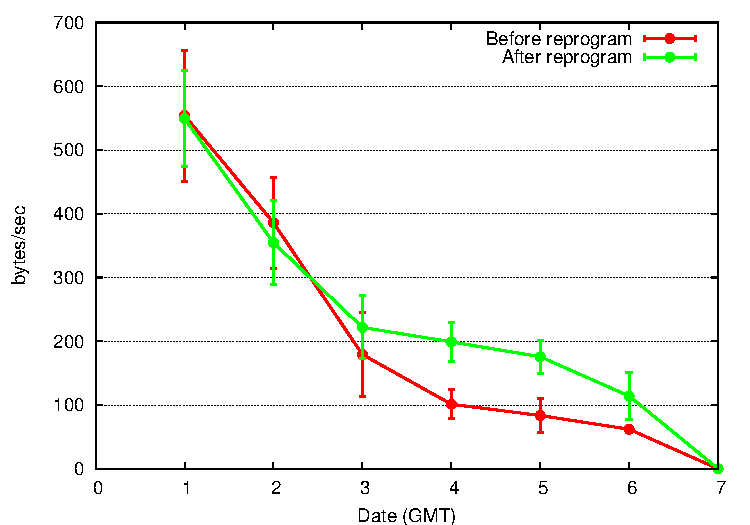
\includegraphics[width=\hsize]{./5-evaluation/figs/performance/fetchspeed-byhops/fetchspeed-oldnew.pdf}
%\end{center}
%\caption{\small{\bf Fetch throughput by node hop count.}
%{\em The throughput of fetch downloads diminishes rapidly as the
%hopcount distance to the node increases. This is due to increased
%packet loss and longer latencies for propagating fetch command
%messages. After reprogramming, fetch throughput increases primarily
%for nodes several hops from the base station.}}
%\label{fig-fetchspeed-byhops}
%\end{figure}

%  - Throughput [MDW]
%    - Bytes/sec
%\begin{figure}[t]
%\begin{center}
%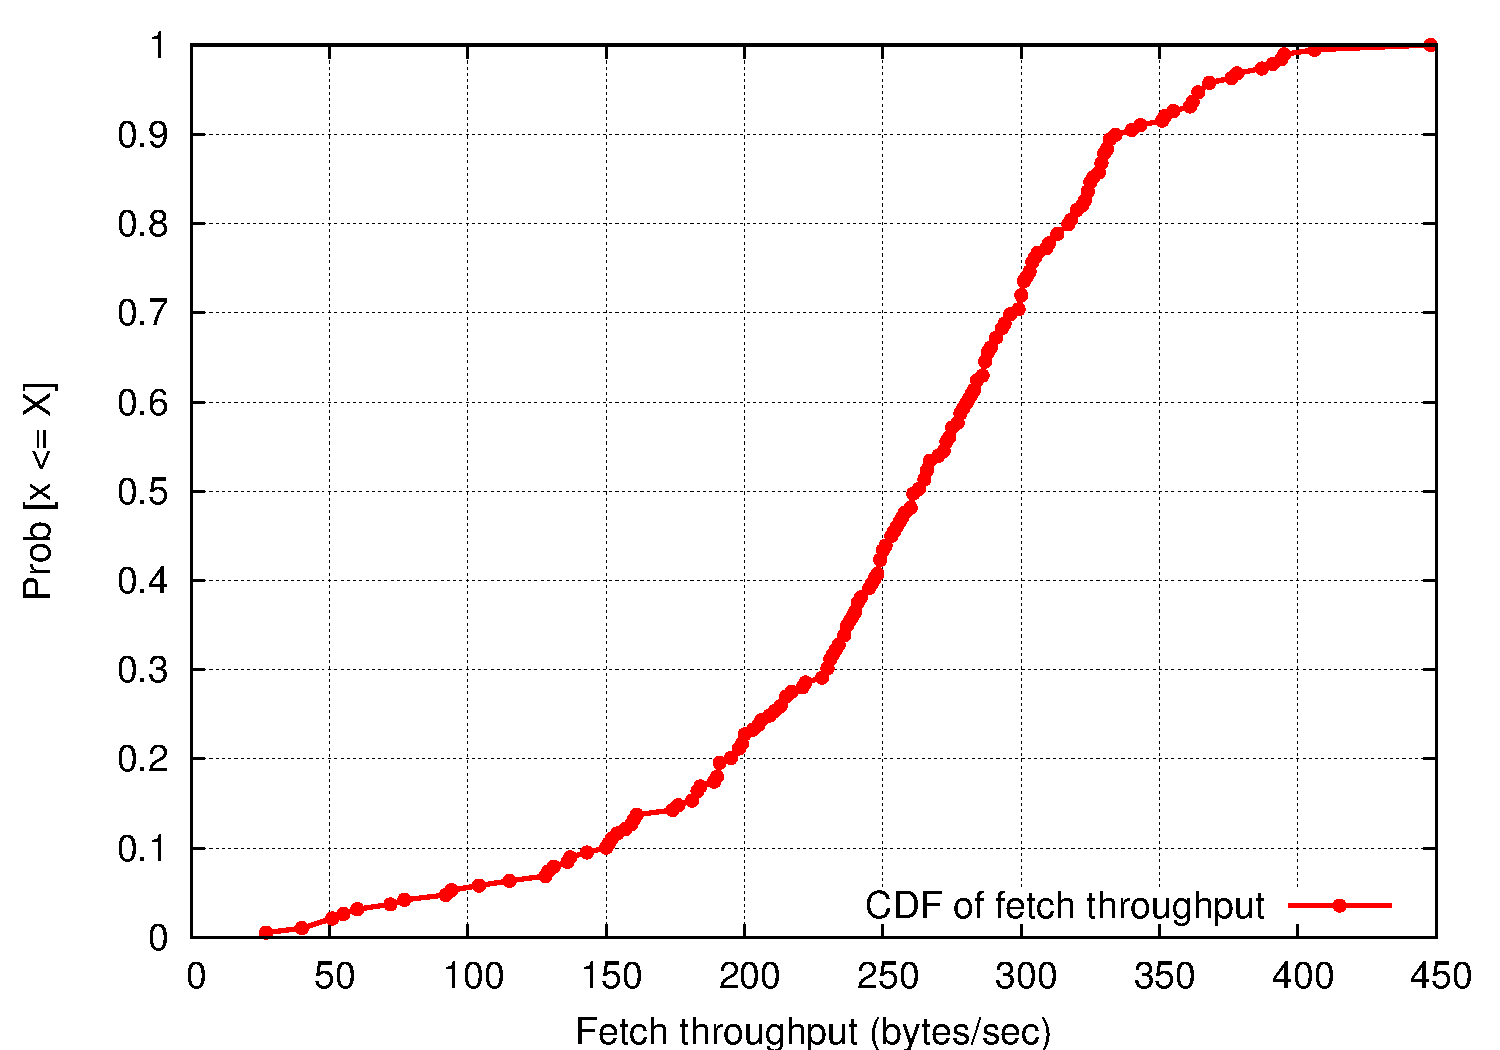
\includegraphics[width=\hsize]{./5-evaluation/figs/performance/fetchspeed/fetchspeed-cdf.pdf}
%\end{center}
%\caption{\small{\bf Fetch throughput.}
%{\em This graph shows a CDF of the the throughput for each fetch
%operation. The median throughput was XXX~bytes/sec and the
%mean~XXX~bytes/sec.}}
%\label{fig-fetchspeed}
%\end{figure}

% 23 Apr 2006 : GWA : Need to discuss this in text... TODO.

%    - Latency for data transfer
%\begin{figure}[t]
%\begin{center}
%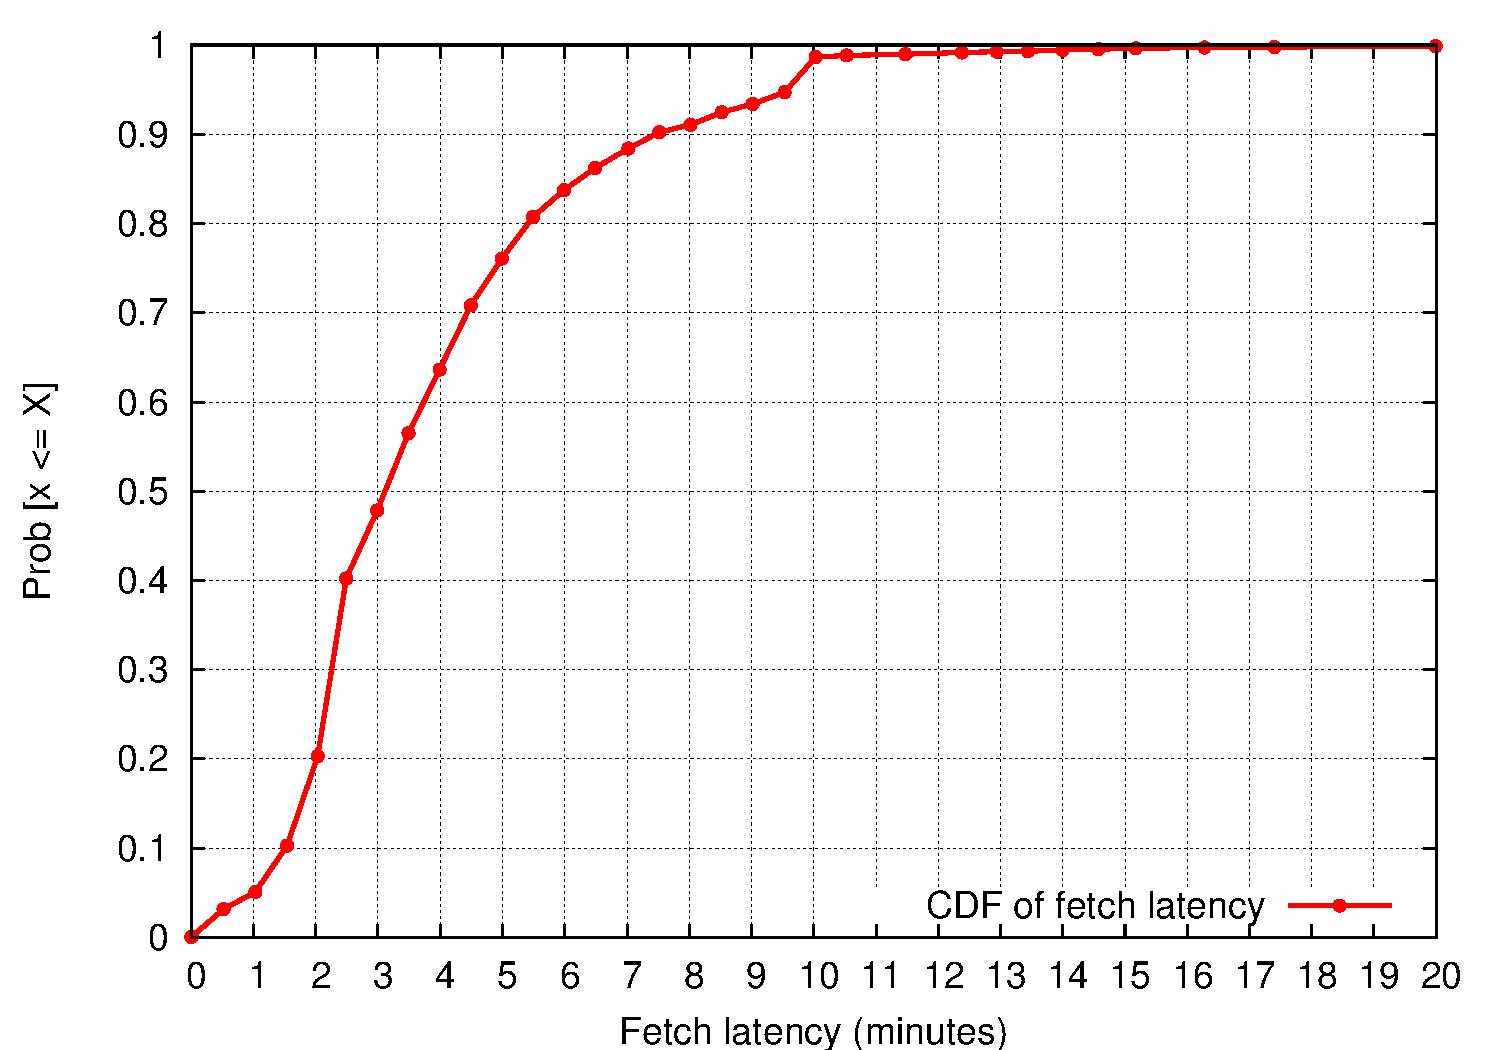
\includegraphics[width=\hsize]{./5-evaluation/figs/performance/fetchlatency/fetch-latency-cdf.pdf}
%\end{center}
%\caption{\small{\bf Fetch latency.}
%{\em This is a CDF of the latency for each fetch operation on a
%per-node basis. The median latency is just over 3~minutes, and the
%maximum latency (in all but a few cases) is 10~minutes.}}
%\label{fig-fetchlatency}
%\end{figure}

%    - Latency by hopcount
%\begin{figure}[t]
%\begin{center}
%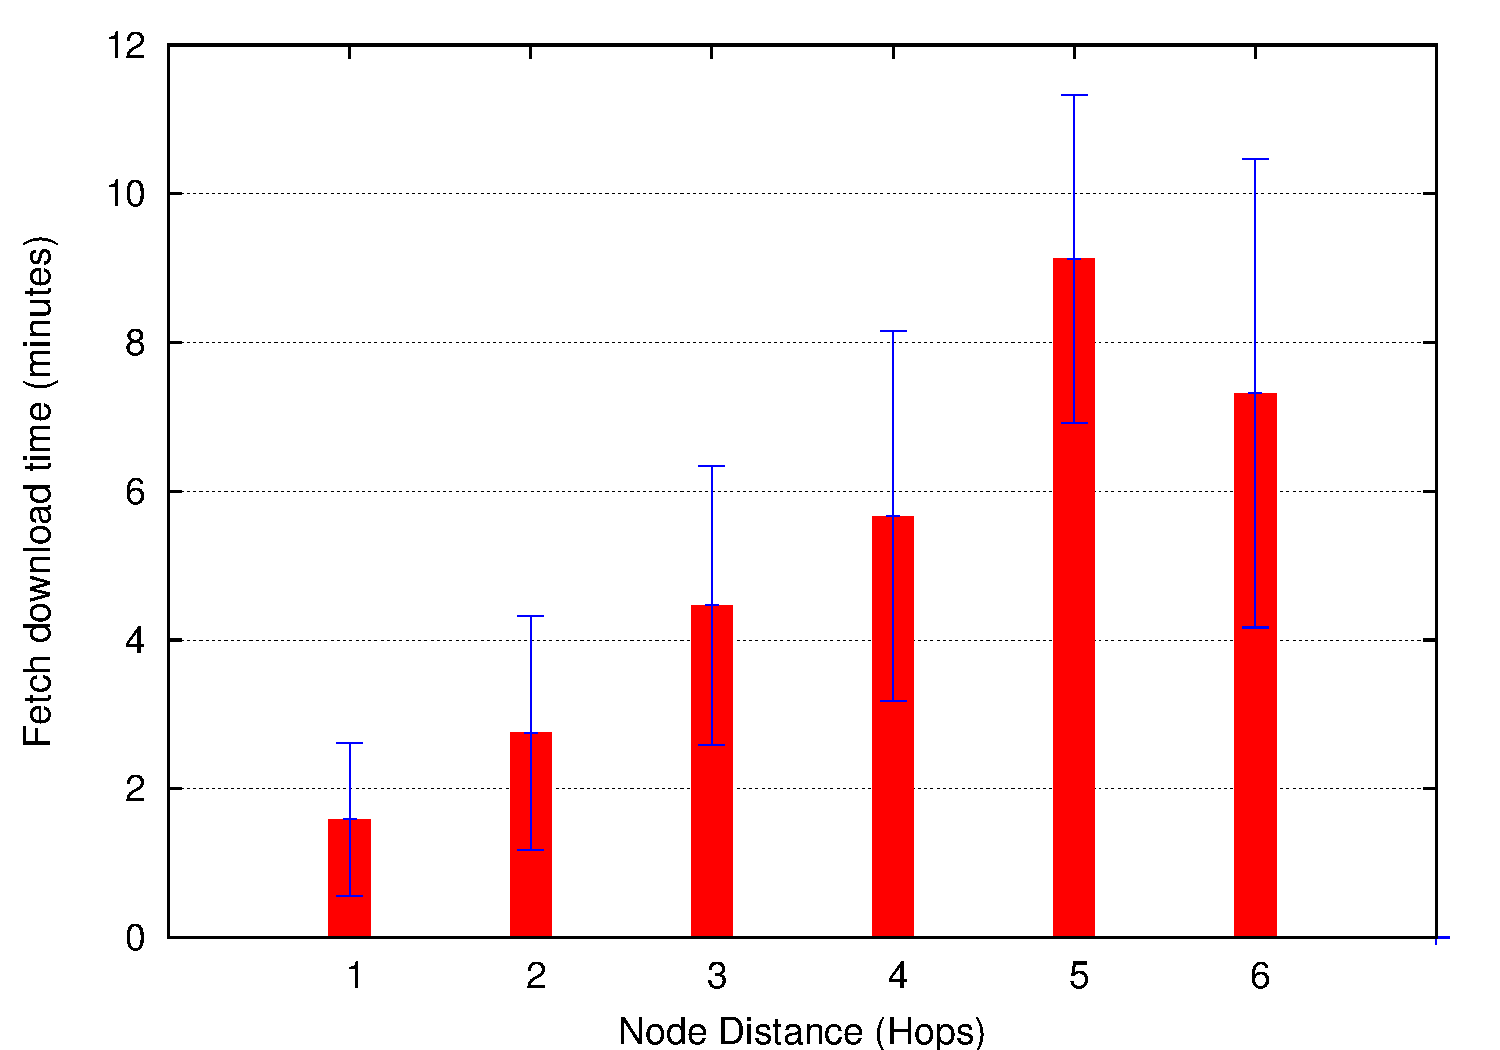
\includegraphics[width=\hsize]{./5-evaluation/figs/performance/fetchlatency/fetchlatency-byhops.pdf}
%\end{center}
%\caption{\small{\bf Fetch latency by hopcount.}
%{\em The latency for a Fetch download depends on the hop distance of
%the node from the root of the spanning tree, which affects both
%command propagation latency and reliability of the routing path.}}
%\label{fig-fetchlatency-byhops}
%\end{figure}


\section{Time Rectification and Accuracy}
\label{evaluation-sec-timing}

\begin{figure}[t!]
\begin{center}
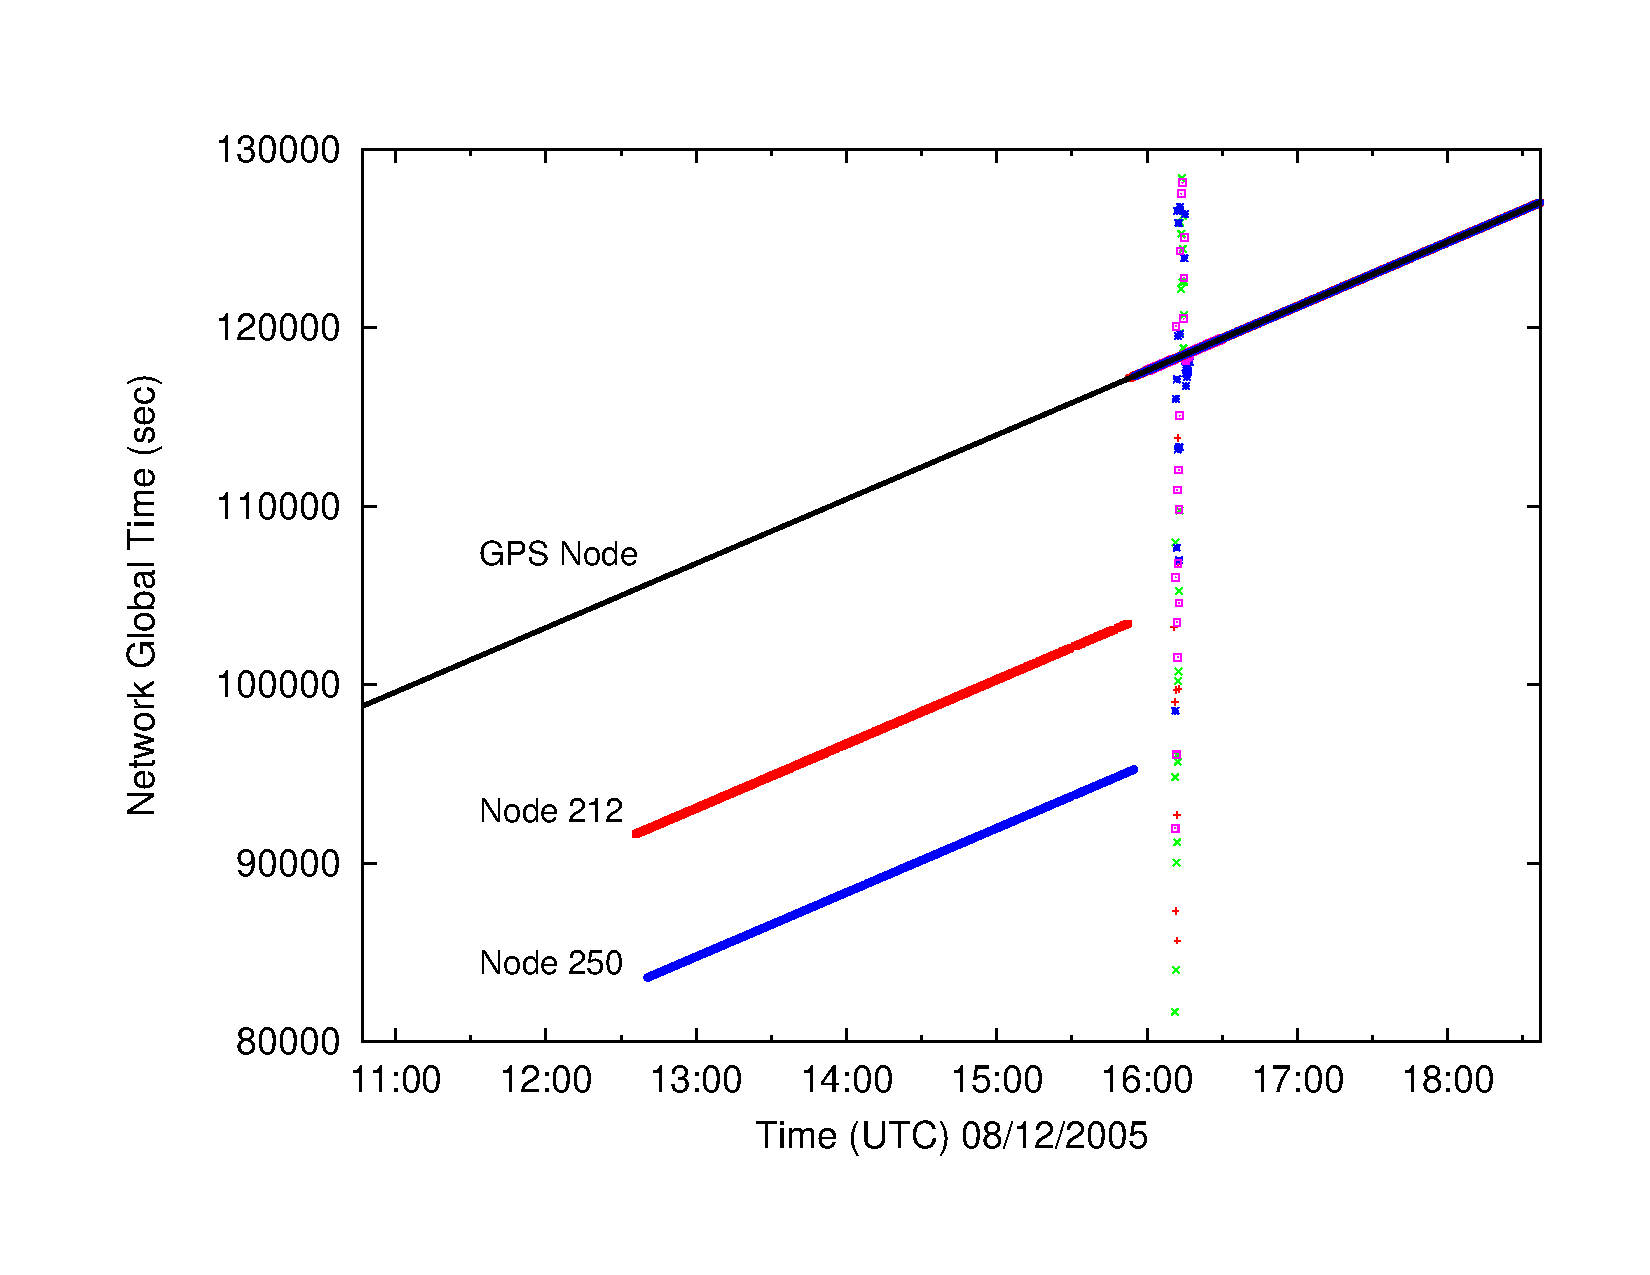
\includegraphics[width=\hsize]{./5-evaluation/figs/timing/MDW/instability/FTSPINSTABILITY.pdf}
\end{center} 
\caption{\textbf{Example of observed FTSP instability.}
The global time value reported by sensor nodes and the GPS node is plotted
against the time that the base station received the corresponding status
messages. All nodes are initially synchronized, but starting at 1230 GMT,
nodes 212~and~250 report incorrect global times for the next 4.5~hours. When
the nodes eventually resynchronize, the global timestamps of other nodes
initially experience some instability.}
\label{evaluation-fig-globaltimeproblem}
\end{figure}

When analyzing seismoacoustic data acquired at volcanoes, accurate timing of
recorded signals is paramount. Studying volcanic source processes
necessitates precisely identifying the arrival time of P-~and S-waves at each
sensor. Also, correlating signals across the sensor array requires accurately
timestamping each sample.  Ideally, timing should be accurate to within one
sample interval, or 10~ms when sampling at 100~Hz.  As described earlier, 
%seismologists typically deploy a GPS receiver at each station. Because GPS
%receivers are expensive and power hungry, 
we opted to use a single GPS receiver and employ a multihop
time-synchronization protocol to establish a global timebase. The protocol
worked well in laboratory experiments. However, it experienced significant
failures in the field, requiring extensive postprocessing of the data to
recover accurate timing for each signal.

In this section, we provide an overview of the time synchronization errors
observed in the field. We then present a novel {\em time rectification}
technique that allows us to recover accurate timing despite protocol
failures.  
%Prior internet measurement work has examined similar techniques for error
%detection and recovery and produced valuable insights and
%advice~\cite{paxson98calibrating,1028824} However, the specific techniques
%do not map directly to our application for several reasons. First, they
%focus more on error detection and do not address rectification.  Second, the
%sensor network time synchronization protocols we deployed are new and have
%goals distinct from common network time-synchronization protocols.
%Additionally, most network measurements can be performed using relative
%times only, whereas the scientific requirements of our application required
%assigning an accurate absolute timestamp to each collected sample.
We evaluate our approach through lab experiments with a known, ground-truth
timebase, and by comparing our signals with signals recorded by the colocated
data loggers. This paper is the first to our knowledge to evaluate the
stability of a multihop time synchronization protocol during a lengthy sensor
network field deployment. 

\subsection{Time synchronization architecture}

We chose to use the Flooding Time Synchronization Protocol
(FTSP)~\cite{ftsp}, an existing protocol developed for wireless sensor nodes.
In the original FTSP work~\cite{ftsp}, timing errors of less than 67~$\mu$sec
were reported for an 11-hop network of Mica2 nodes.  We verified in our
testbed that FTSP provided a 90th-percentile time error of under 2.1~ms in a
5-hop linear network of TMote Sky nodes.

A single MicaZ sensor node was used as the root of the FTSP synchronization
tree. It interfaced to a Garmin GPS receiver and received a 1~Hz interrupt
synchronized to within 1~$\mu$sec of the GPS ``pulse per second'' signal.
When the interrupt is raised, the node records the GPS time and corresponding
FTSP global time and sends a short message containing this information to the
base station.  Each sensor node runs the FTSP protocol which maintains a
global timebase. Every 10~sec, each node records its local time and the
corresponding FTSP global time, sending this information in its status
message to the base station. Finally, as each node records data, the first
sample of each block is marked with the node's local time. After downloading
data from each node following an event, this local time can be used to
recover the time for each sample in the block.

Therefore, we have three relevant timebases: the {\em local time} at each
node; the {\em global time} established by the FTSP protocol; and the {\em
GPS time} recorded by the FTSP root. The information in the nodes' status
messages can be used to map local time to global time, and the information in
the GPS node's status messages can be used to map global time to GPS-based
GMT.

\subsection{FTSP failures in the field}
\label{evaluation-timing-deploymentfailures}

In the absence of failures, this mapping would be a straightforward process.
However, in the field, we noticed that nodes would occasionally lose
synchronization with the rest of the network and report FTSP global times
with significant errors, sometimes exceeding several hours. We suspect that
the sparse deployment conditions at the volcano might have led to different
behavior in the time synchronization protocol than in the lab. For example,
occasional message loss or failure of a neighbor could cause the node's
global time to drift from the rest of the network.  However, in lab tests
that constrained the network topology we did not observe these instabilities.

Figure~\ref{evaluation-fig-globaltimeproblem} shows an example of the FTSP
instability observed in the field. The global time reported by two nodes
suddenly jumps off by several hours, and the nodes do not resynchronize until
rebooted 4.5~hours later.  It turns out that two bugs conflated to cause this
problem.  First, it was discovered that the TinyOS clock driver would
occasionally return bogus local timestamps.  This bug was fixed in February
2006, several months after our deployment.  Second, FTSP does not check the
validity of synchronization messages, so a node reading an incorrect value
for its local clock can corrupt the state of other nodes, throwing off the
global time calculation.  To our knowledge, few if any sensor network
deployments have attempted to use network time synchronization protocols for
extended periods.  In addition, ours may have been the first deployment of
FTSP on the TMote Sky platform where the clock driver bug manifested itself. 

\begin{figure}[t]
\label{evaluation-fig-rectificationcartoon}
\begin{center}
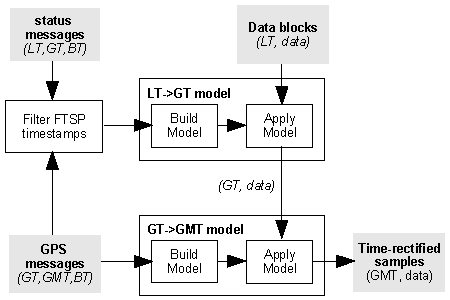
\includegraphics[width=0.8\hsize]{./5-evaluation/figs/timing/RectificationCartoon/cartoon.pdf}
\end{center}
\caption{\textbf{Time rectification process overview.}}
\end{figure}

The failures of the time synchronization protocol make establishing the
correct GPS-based timestamp for each data sample extremely challenging. Our
{\em time rectification} approach filters and remaps recorded timestamps to
accurately recover timing despite these failures.  The time rectification
process is illustrated in Figure~\ref{evaluation-fig-rectificationcartoon}.
The first step is to {\em filter} the global timestamps recorded by each
node, discarding bogus data. Second, we build a model mapping the local time
on each node to FTSP-based global time.  Third, we use the GPS timestamp
information to build a second model mapping FTSP time to GMT. Finally, both
models are applied to the timestamps recorded in each data block producing a
GMT time for each sample.

\subsection{Timestamp filtering}
\label{evaluation-subsection-filtering}

We begin by filtering out status messages appearing to contain incorrect
global timestamps. To do this, we correlate global timestamps from each node
against a common reference timebase and reject those that differ by more than
some threshold.  For this, we use the base station laptop's local time, which
is {\em only} used for filtering FTSP timestamps, not for establishing the
correct timing. The filtering process in is many ways similar to prior
work~\cite{paxson98calibrating,1028824} on detecting adjustments in
network-synchronized clocks.

We use the following abbreviations: {\em LT} is the local time of a node;
{\em GT} is the FTSP global time; {\em BT} is the base station's local time;
and {\em GMT} is the true GMT from the GPS signal.  Each GPS status message
logged by the base station consists of the triple {\em (GT, GMT, BT)}.  We
use linear regression on this data to produce a reference timebase mapping
{\em BT} to {\em GT}.\footnote{We assume that the global time reported by the
GPS node is always correct; indeed, the definition of ``global time'' is the
FTSP time reported by the GPS node. We verified that the FTSP instability
affecting the sensor nodes did not occur on the GPS node, most likely because
the MicaZ uses a different processor that is unaffected by the clock driver
bug.} For each node status message logged by the laptop {\em (LT, GT, BT)},
we map {\em BT} to the expected $\mathit{GT}_{\mathit{ref}}$ using the
reference timebase. If $ \mid \mathit{GT}_{\mathit{ref}} - \mathit{GT} \mid >
\delta$, we discard the status message from further consideration.  We use a
threshold of $\delta = 1$~sec.  Although radio message propagation and delays
on the base station can affect the {\em BT} for each status message, a small
rejection threshold $\delta$ makes it unlikely that any truly incorrect FTSP
timestamps pass the filter. Indeed, of the 7.8\% of timestamps filtered out,
the median {\em GT} error was 8.1~hours.


%\begin{figure}[t]
%\begin{center}
%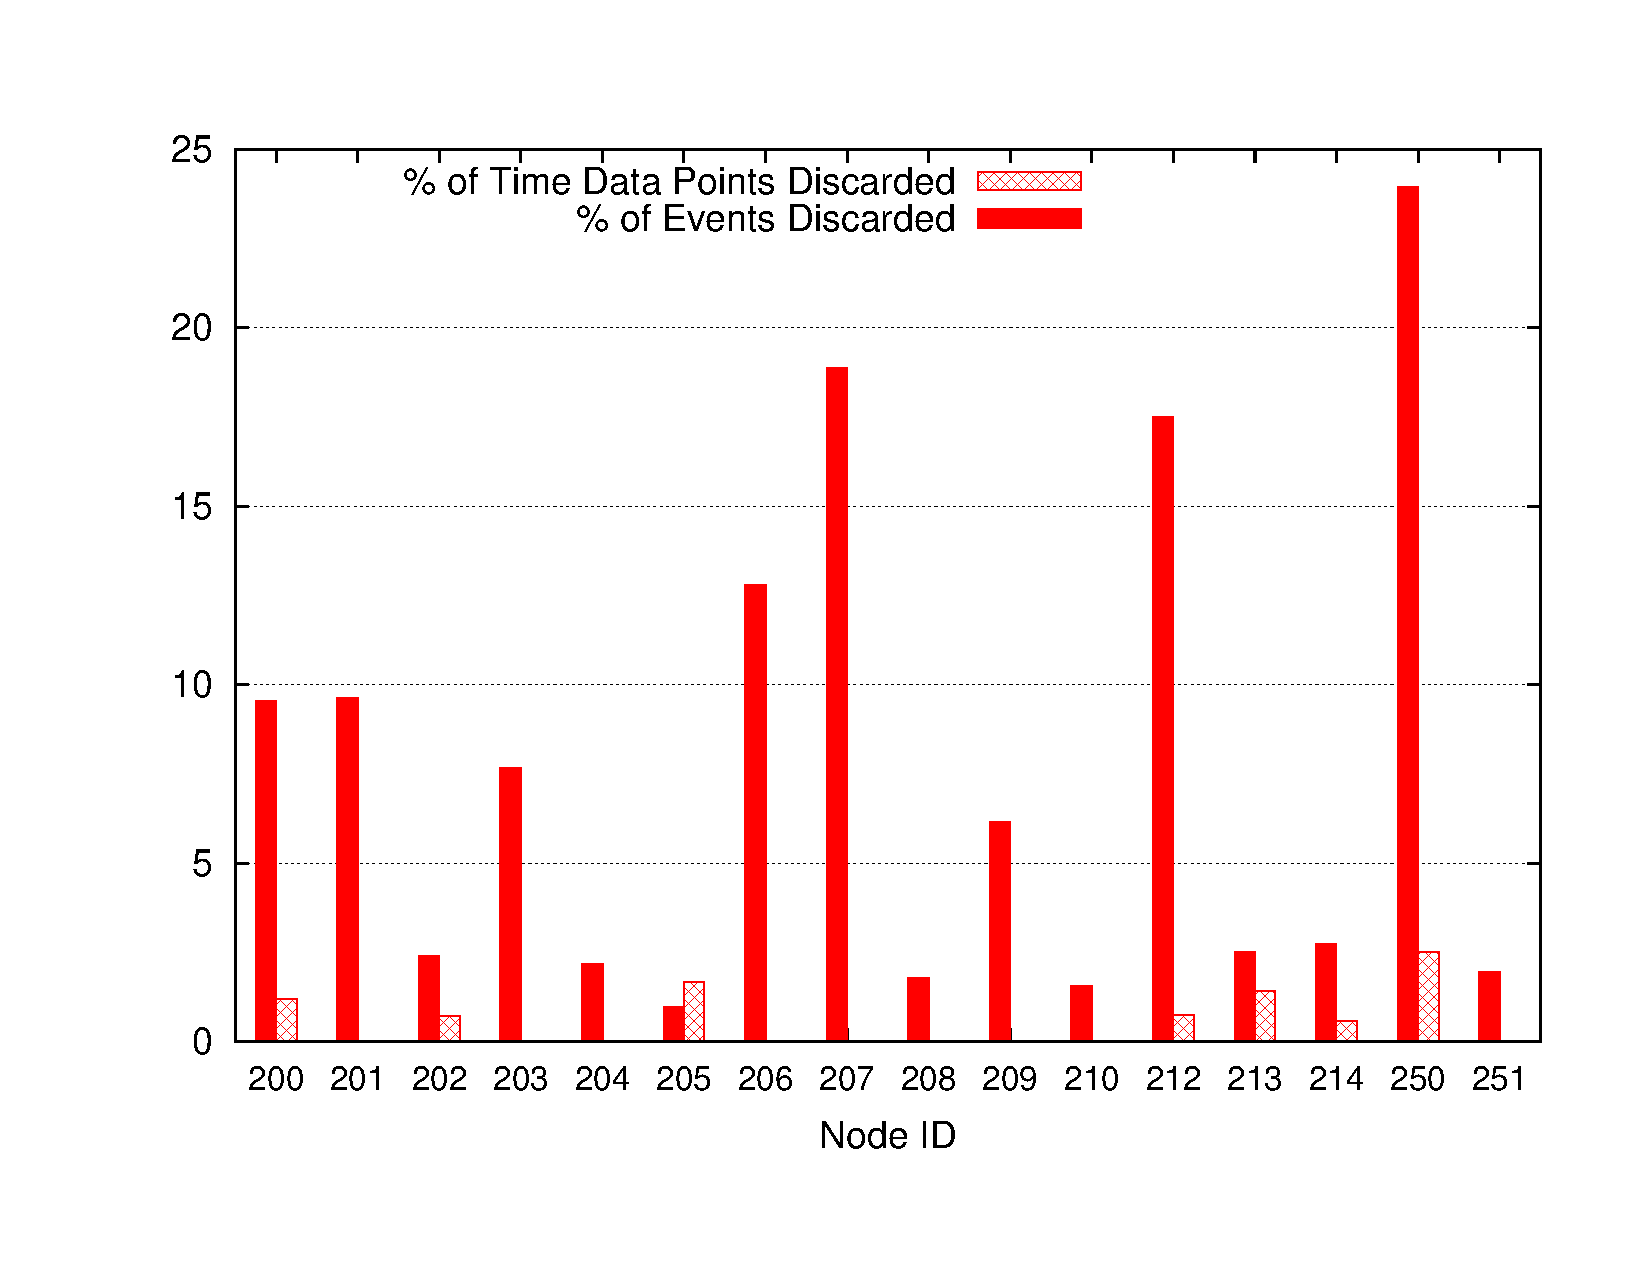
\includegraphics[width=\hsize]{./5-evaluation/figs/timing/ComparisonFigure/COMPARISONFIGURE.pdf}
%\end{center}
%\caption{\small{\bf Percentage of timestamps discarded by filtering versus
%percentage of events discarded because of timing failures:}
%{\em Overall, the filter rejected 7.9\% of the time 
%stamps reported by sensor nodes. Certain nodes, such as
%node~250, had an unusually large number of FTSP failures. However, the time
%rectification process can hide FTSP errors, as seen by the fact that overall
%we only had to discard 0.8\% of events because of bad timing.}}
%\label{fig-ftspdown}
%\end{figure}

\subsection{Timestamp rectification}
\label{evaluation-section-timerectification}

\begin{figure}[t]
\label{evaluation-fig-rectificationprocess}
\begin{center}
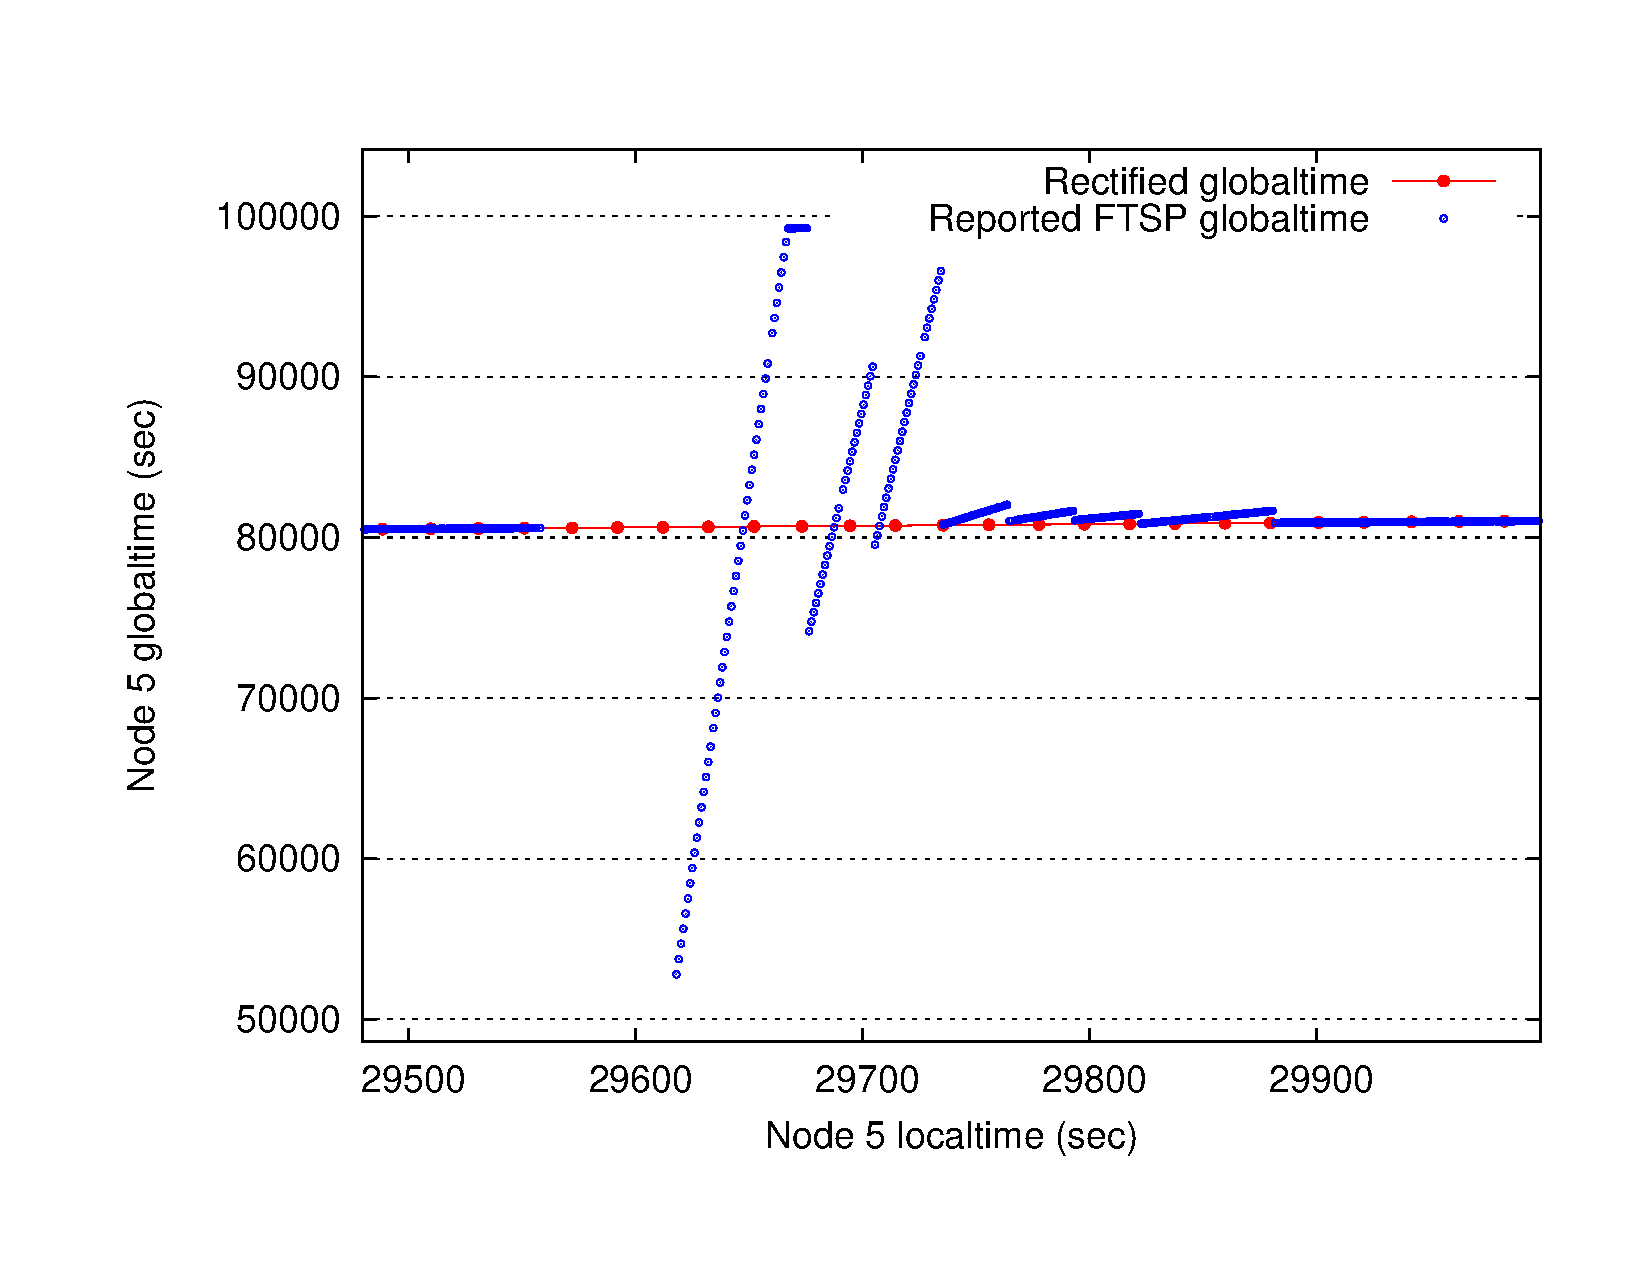
\includegraphics[width=\hsize]{./5-evaluation/figs/timing/MDW/rectification/rectify.pdf}
\end{center}
\caption{\textbf{Time rectification example.}
The raw (LT, GT) pairs collected from the node show that it experiences a
period of FTSP instability.  The time rectification process removes the
errant timestamps creating an accurate mapping between LT and GT created
using a linear regression on the remaining timestamps.}
\end{figure}

The goal of {\em time rectification} is to assign a GMT timestamp to each
sample in the recorded data. In order to do so, we build two models: one
mapping a node's local time to global time, and another mapping global time
to GMT. 

%\begin{figure}[t]
%\begin{center}
%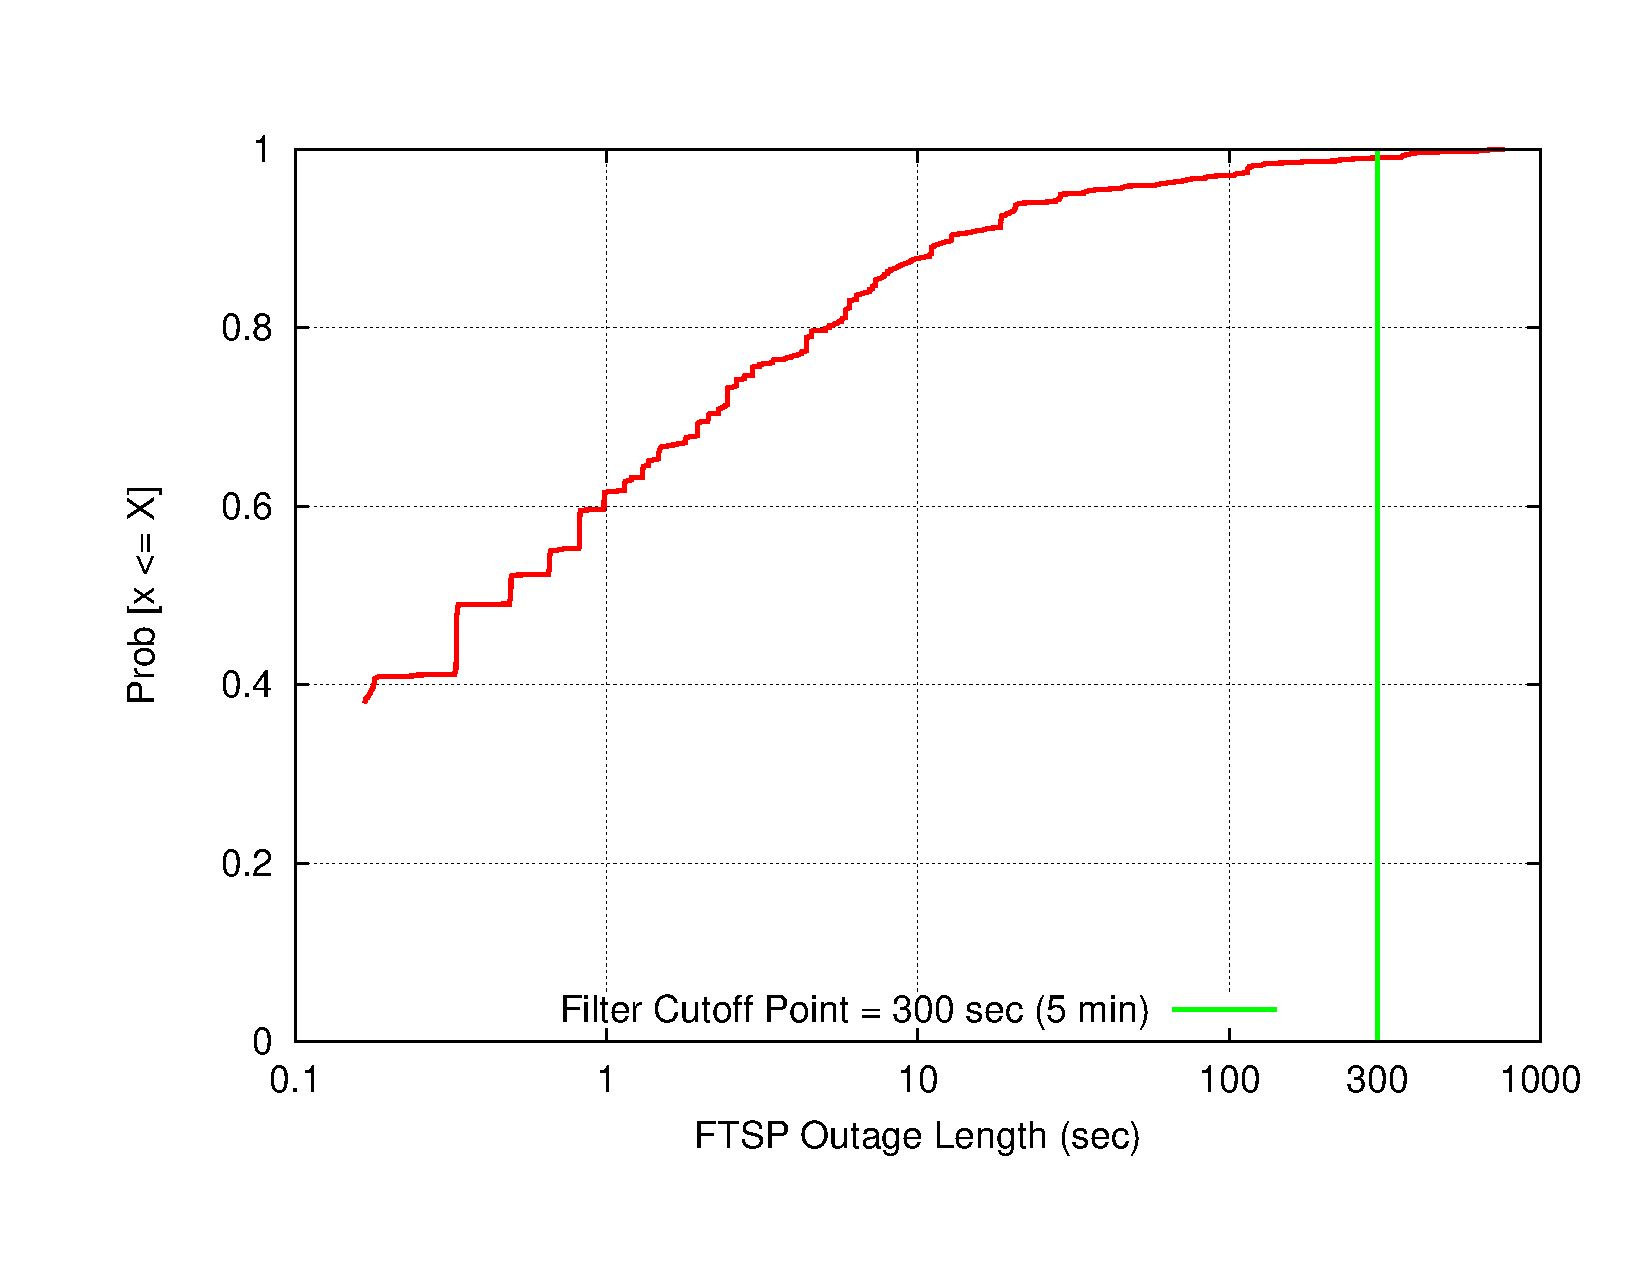
\includegraphics[width=\hsize]{./5-evaluation/figs/timing/FTSPRuns/FTSPDOWN-RUNS-CDF.pdf}
%\end{center}
%\caption{\small{\bf Run lengths for discarded timestamps:} {\em This is a CDF
%of the length of consecutive runs of timestamps discarded by our filter. As
%the figure shows, only 1\% of runs exceed our cutoff threshold of 5~minutes.
%The majority of runs are short and can be be bridged by the time
%rectification process.}}
%\label{fig-ftspdown-runs-cdf}
%\end{figure}

From those status messages that pass the filter, we build a piecewise linear
model mapping {\em LT} to {\em GT} using a series of linear regressions.
Models are constructed for each node separately, since local times vary
significantly between nodes.  Each regression spans up to 5~minutes of data
and we initiate a new regression if the gap between subsequent {\em (LT, GT)}
pairs exceeds 5~minutes.  Each interval must contain at least two valid
status messages to construct the model.  We take the {\em LT} value stored in
each data block and use this model to recover the corresponding {\em GT}
value.

The next step is to map global time to GMT. Each of the GPS node's status
messages contain a {\em (GT, GMT)} pair. As above, we build a piecewise
linear model mapping {\em GT} to {\em GMT}, and apply this model to the {\em
GT} values for each data block. Finally, we assign a GMT value to each sample
contained in the block, using linear interpolation between the GMT values
assigned to the first sample in each block.  This process makes no
assumptions about sampling rate, which varies slightly from node to node due
to clock drift.

\subsection{Evaluation}
\label{evaluation-timing-postdeployment}

Evaluating this time rectification process has proved difficult, primarily
because we have no ground truth for the timing of the signals recorded in the
field. However, by reproducing the deployment conditions in the lab, we have
been able to measure the accuracy of the recovered timing in a controlled
setting. In addition, as described earlier, two GPS-synchronized data loggers
were colocated with our sensor network, providing us the opportunity to
directly compare our time-rectified signals with those recorded by
conventional instrumentation.

Our first validation took place in the lab. Feeding the output of a signal
generator to both a miniature version of our sensor network and to a
Reftek~130 data logger allowed us to directly compare the data between both
systems. The miniature network consisted of a single sensor node, routing
gateway, and GPS receiver node. The same software was used as in the field
deployment. The Reftek~130 logs data to a flash memory card and timestamps
each sample using its own GPS receiver. The Reftek~130 is commonly used in
volcano field studies and its timing accuracy has been extensively validated.

The results showed a consistent 15~ms offset between the time-rectified
signals recorded by the sensor node and the Reftek data logger.  We
discovered that this offset was due to delays introduced by the digital
filtering performed by the ADC on our sensor board. Adjusting for this delay
resulted in an indiscernible offset between the sensor node and Reftek
signals. While this experiment does not reproduce the full complexity of our
deployed network, it does serve as a baseline for validation.

In the second lab experiment, we set up a network of 7~sensor nodes in a
6-hop linear topology. The topology is enforced by software, but all nodes
are within radio range of each other, making it possible to stimulate all
nodes simultaneously with a radio message.  Each node samples data and sends
status messages using the same software as the field deployment. The FTSP
root node periodically transmits a beacon message. On reception of the
beacon, each node records the FTSP global timestamp of the message reception
time (note that reception of the beacon message is not limited by the
software-induced topology).  Because we expect all nodes to receive this
message at the same instant, modulo interrupt latency jitter, we expect the
FTSP time recorded by each node to be nearly identical. The FTSP root also
records the time that the beacon was transmitted, accounting for MAC delay.
The experiment ran for 34~hours, during which time FTSP experienced
instabilities similar to those seen during our deployment.

\begin{figure}[t]
\label{evaluation-fig-time-rect-lab}
\begin{tabular}{|lll|} \hline
                  & {\bf Raw error} & {\bf Rectified error} \\ \hline
{\bf  1 hop}, 50th percentile & 1.52 ms & 1.42 ms \\ 
{\bf 1 hop}, 90th percentile & 9.86 ms & 6.77 ms \\ \hline 
{\bf 6 hops}, 50th percentile & 2.63 ms & 2.18 ms \\ 
{\bf 6 hops}, 90th percentile & 13.5 ms & 6.8 ms \\ \hline 
\end{tabular} \\
\caption{\textbf{Timestamp errors in a 6-hop lab testbed.}
This table shows the 50th and 90th-percentile timing errors on both the raw
FTSP timestamps, and rectified timestamps.}
\end{figure}

This allows us to compare the {\em true} global time of each beacon message
transmission and the {\em apparent} global time on each receiving node, both
before and after subjecting the data to our time rectification process.  We
call the difference between the true and apparent times the {\em timestamp
error}. Figure~\ref{evaluation-fig-time-rect-lab} shows the results for nodes
one and six hops away from the FTSP root.  After rectification, 99.9\% of the
errors for the one-hop node and 93.1\% of the errors for the six-hop node
fall within our 10~ms error envelope.

\clearpage

%\begin{figure}[t]
%\begin{center}
%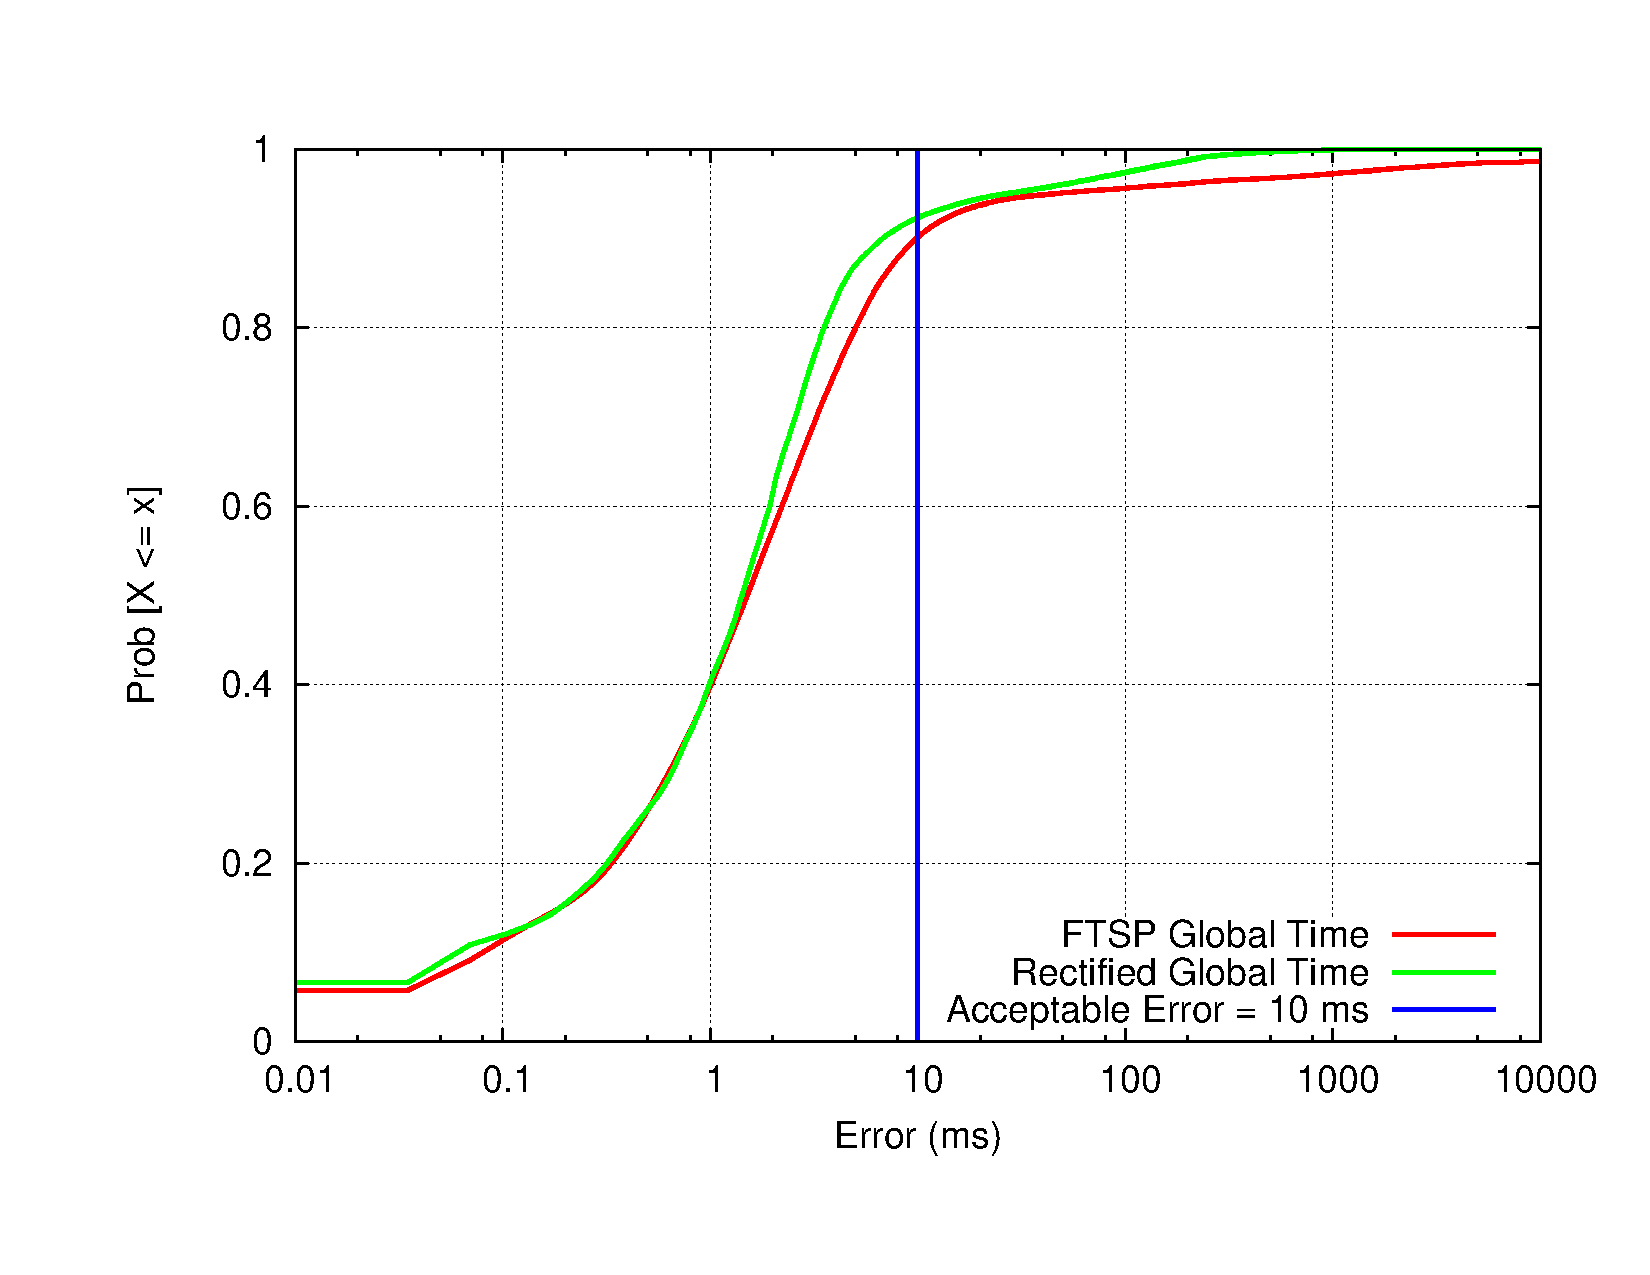
\includegraphics[width=\hsize]{./5-evaluation/figs/timing/TelosLabNew/FTSPVMAPPEDNODE0.pdf}
%{\small {\bf (a, 1 hop)}}
%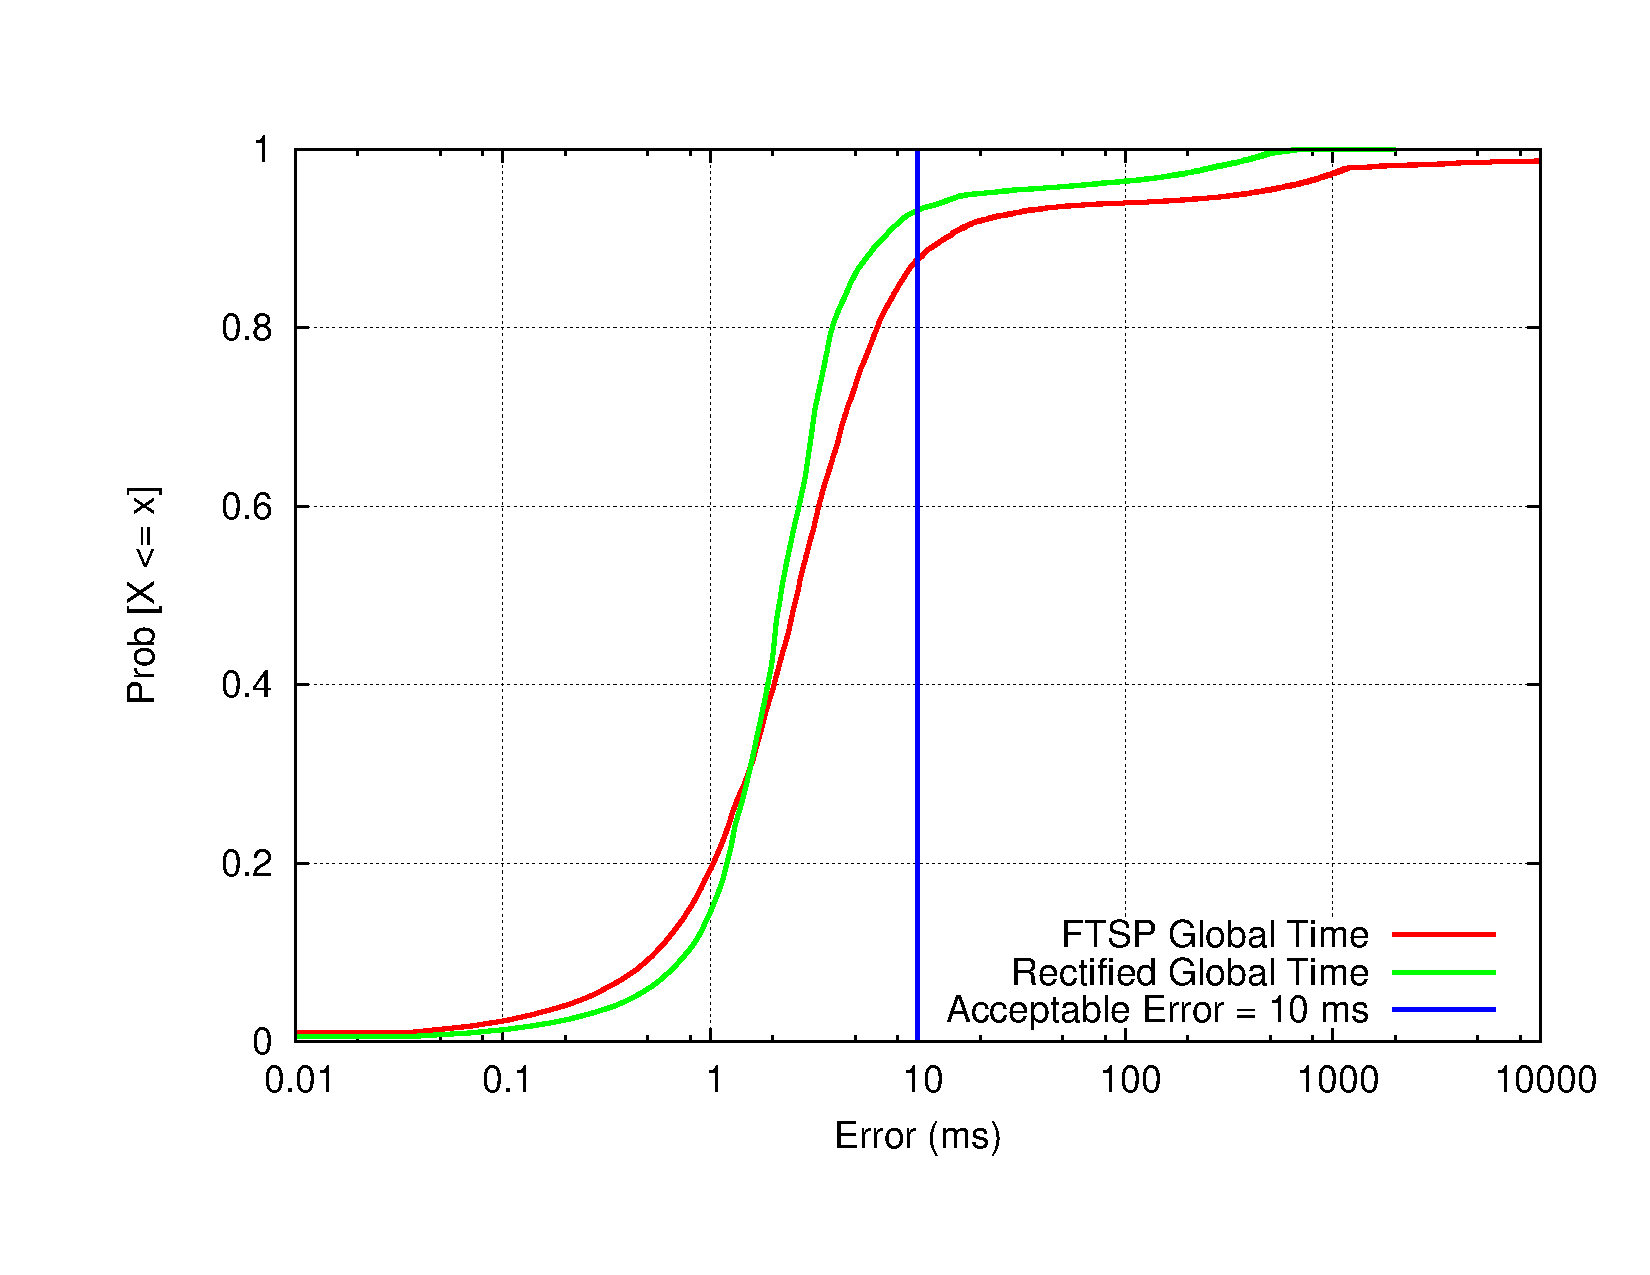
\includegraphics[width=\hsize]{./5-evaluation/figs/timing/TelosLabNew/FTSPVMAPPEDNODE6.pdf}
%{\small {\bf (b, 6 hops)}}
%\end{center}
%\caption{\small{\bf Testbed Comparison of FTSP and Time Rectification Errors}
%{\em During the experiment described in Section~\ref{timing-postdeployment}
%we used periodic heartbeat messages to collect synchronous local time, global
%time pairs across the network.  These graphs show the distribution of the
%FTSP error and the mapping error with respect to the ``true'' global time,
%that is the stamp recorded on the broadcast node when it sent the message,
%for two nodes.  Figure (a) shows the distribution for the node 1 hop away
%  from the root of the FTSP tree.  For this node, 96.4\% of the FTSP global
%  timestamps and 99.9\% of the mapped global timestamps were within 10~ms of
%  the true global time. Figure (b) shows the same distribution for the node 6
%  hops from the root.  For this node, 87.6\% of the FTSP global timestamps
%  and 93.1\% of the mapped global timestamps were within 10~ms of the true
%  global time. We had a difficult time reproducing the long periods of FTSP
%  instability experienced in the field in the testbed setting.}}
%\label{fig-benchtest}
%\end{figure}

% 20 Apr 2006 : GWA : UNUSED FIGURES.

%\begin{figure}[t]
%  \begin{small}
%    \begin{center}
%      \begin{tabular}{|cc|} \hline
%        {\bf Event} & {\bf Shift} \\ \hline
%2005-08-13\_03.38.08 & 29 \\
%2005-08-13\_06.16.46 & -45 \\
%2005-08-13\_08.17.51 & 29 \\
%2005-08-13\_15.24.58 & -36 \\
%2005-08-15\_04.48.27 & -43 \\
%2005-08-15\_07.07.52 & 46 \\
%2005-08-15\_09.11.28 & -29 \\
%2005-08-15\_16.04.37 & 48 \\
%2005-08-16\_04.04.56 & -21 \\
%2005-08-16\_09.45.14 & 15 \\
%2005-08-17\_05.07.31 & -26 \\
%2005-08-17\_14.00.43 & -26 \\
%2005-08-17\_16.48.26 & -71 \\
%2005-08-18\_00.52.31 & 11 \\
%2005-08-18\_03.43.05 & 41 \\
%2005-08-18\_04.54.30 & 23 \\
%2005-08-18\_06.26.50 & 19 \\
%2005-08-18\_17.59.49 & 45 \\
%2005-08-18\_21.33.01 & 8 \\
%2005-08-19\_00.16.22 & -7 \\
%2005-08-19\_01.52.09 & -25 \\
%2005-08-19\_02.33.30 & -58 \\
%2005-08-15\_19.29.08 & 48 \\
%2005-08-17\_00.22.39 & -55 \\
%2005-08-17\_02.09.47 & -27 \\
%2005-08-18\_13.28.54 & 9 \\
%2005-08-18\_14.23.06 & 25 \\
%2005-08-18\_15.31.06 & -42 \\
%        \hline
%      \end{tabular}
%    \end{center}
%  \end{small}
%\caption{\small{\bf Hand-picked Shifts Between Node 213 and Reftek} {\em For
%each event that we had signals from both Node 213 and the RVEN, the Reftek
%station located nearby, we used {\tt MATLAB}'s {\tt xcorr} function to
%produce some possible time shifts between each signal.  We then examined each
%shift by hand to pick the best one.  An example of this process can be seen
%in Figure~\ref{fig-rvenv213}. This table shows the shifts for all events for
%which we had paired data. As can be seen most are under 50~ms, the greatest
%possible shift possible given the distance between the stations.}}
%\label{fig-rvenv213table}
%\end{figure}

%\begin{figure}[t]
%\begin{center}
%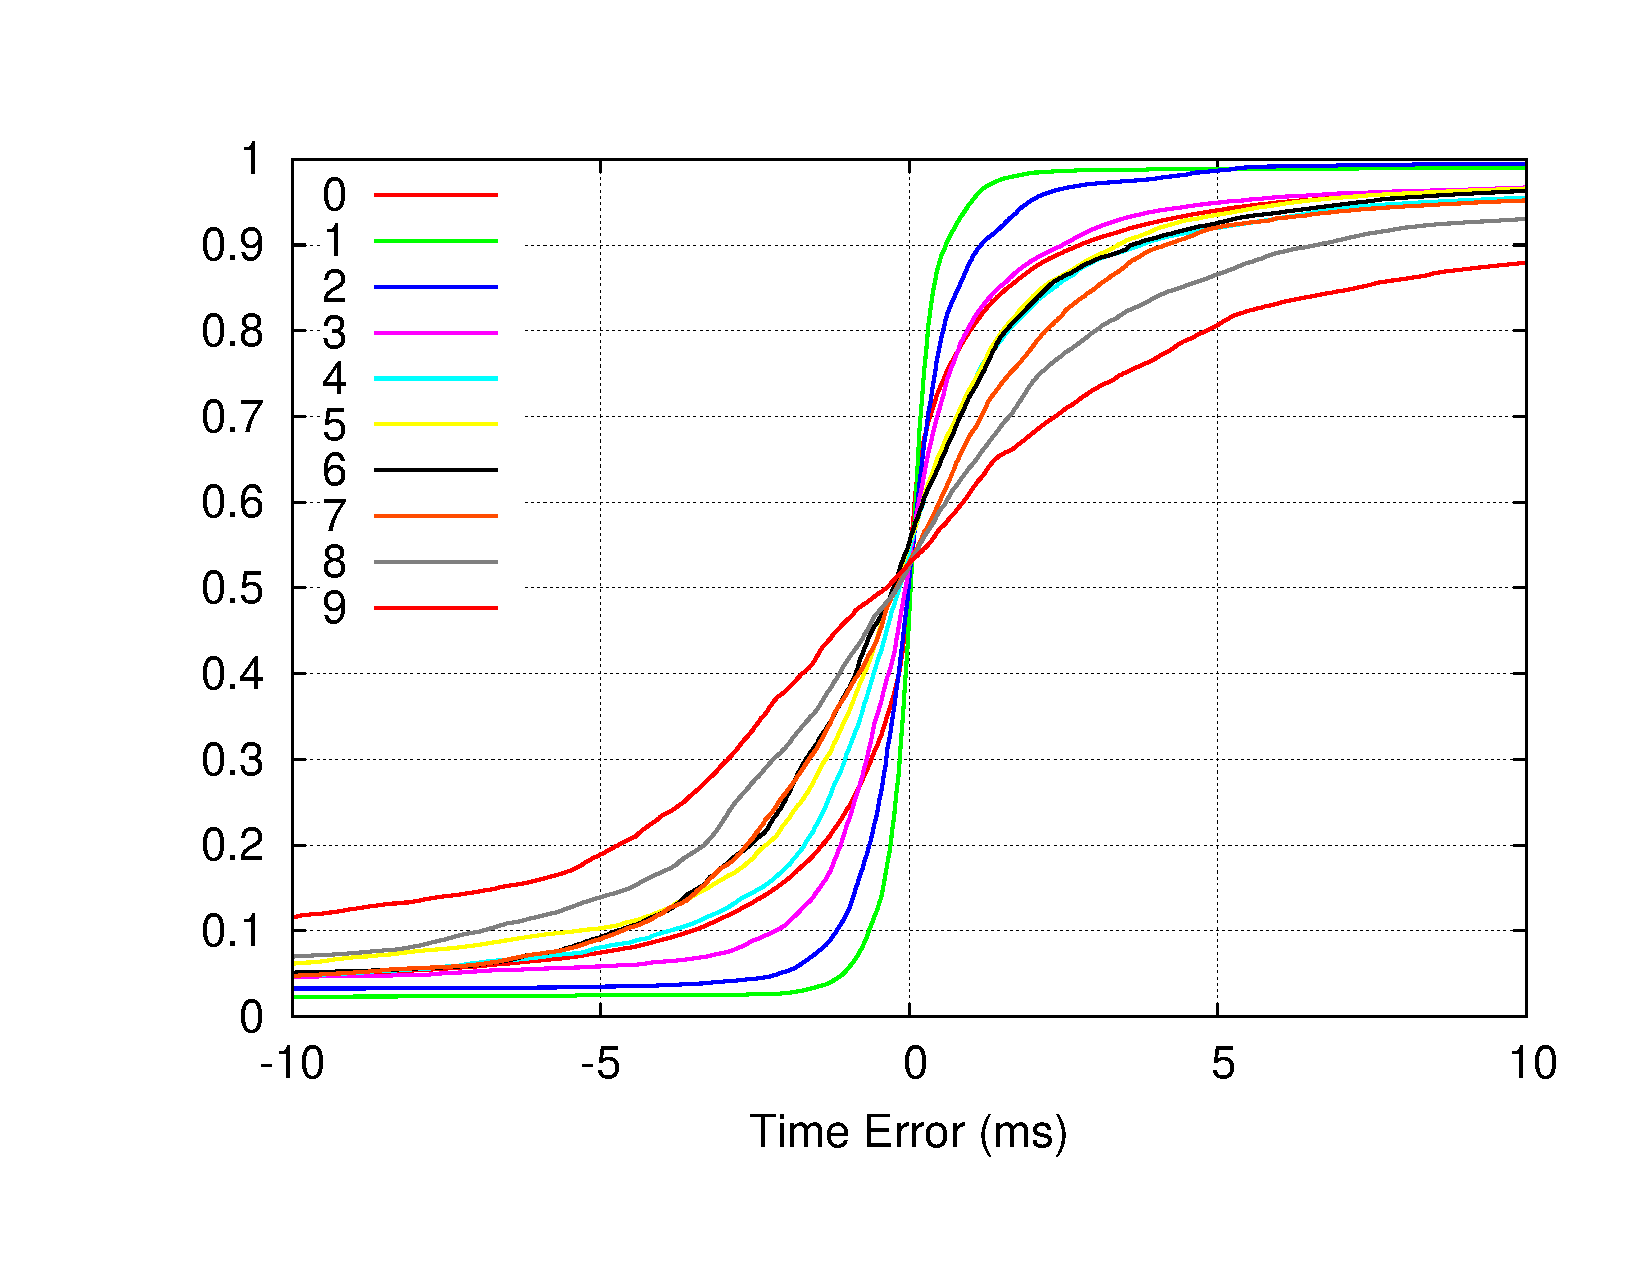
\includegraphics[width=\hsize]{./5-evaluation/figs/timing/TelosLabTiming/MAPPINGERROR.pdf}
%\end{center}
%\caption{\small{\bf Distribution of Bench Test FTSP Mapped Global to Reported
%Global Time Errors}
%{\em \GWAnote{I don't think that this graph should be in the paper, so I'm
%not commenting it.  The rest of this stuff is confusing enough and this
%doesn't say much because the errors are not additive!}}}
%\label{fig-mappingerror}
%\end{figure}

%\begin{figure}[t]
%\begin{center}
%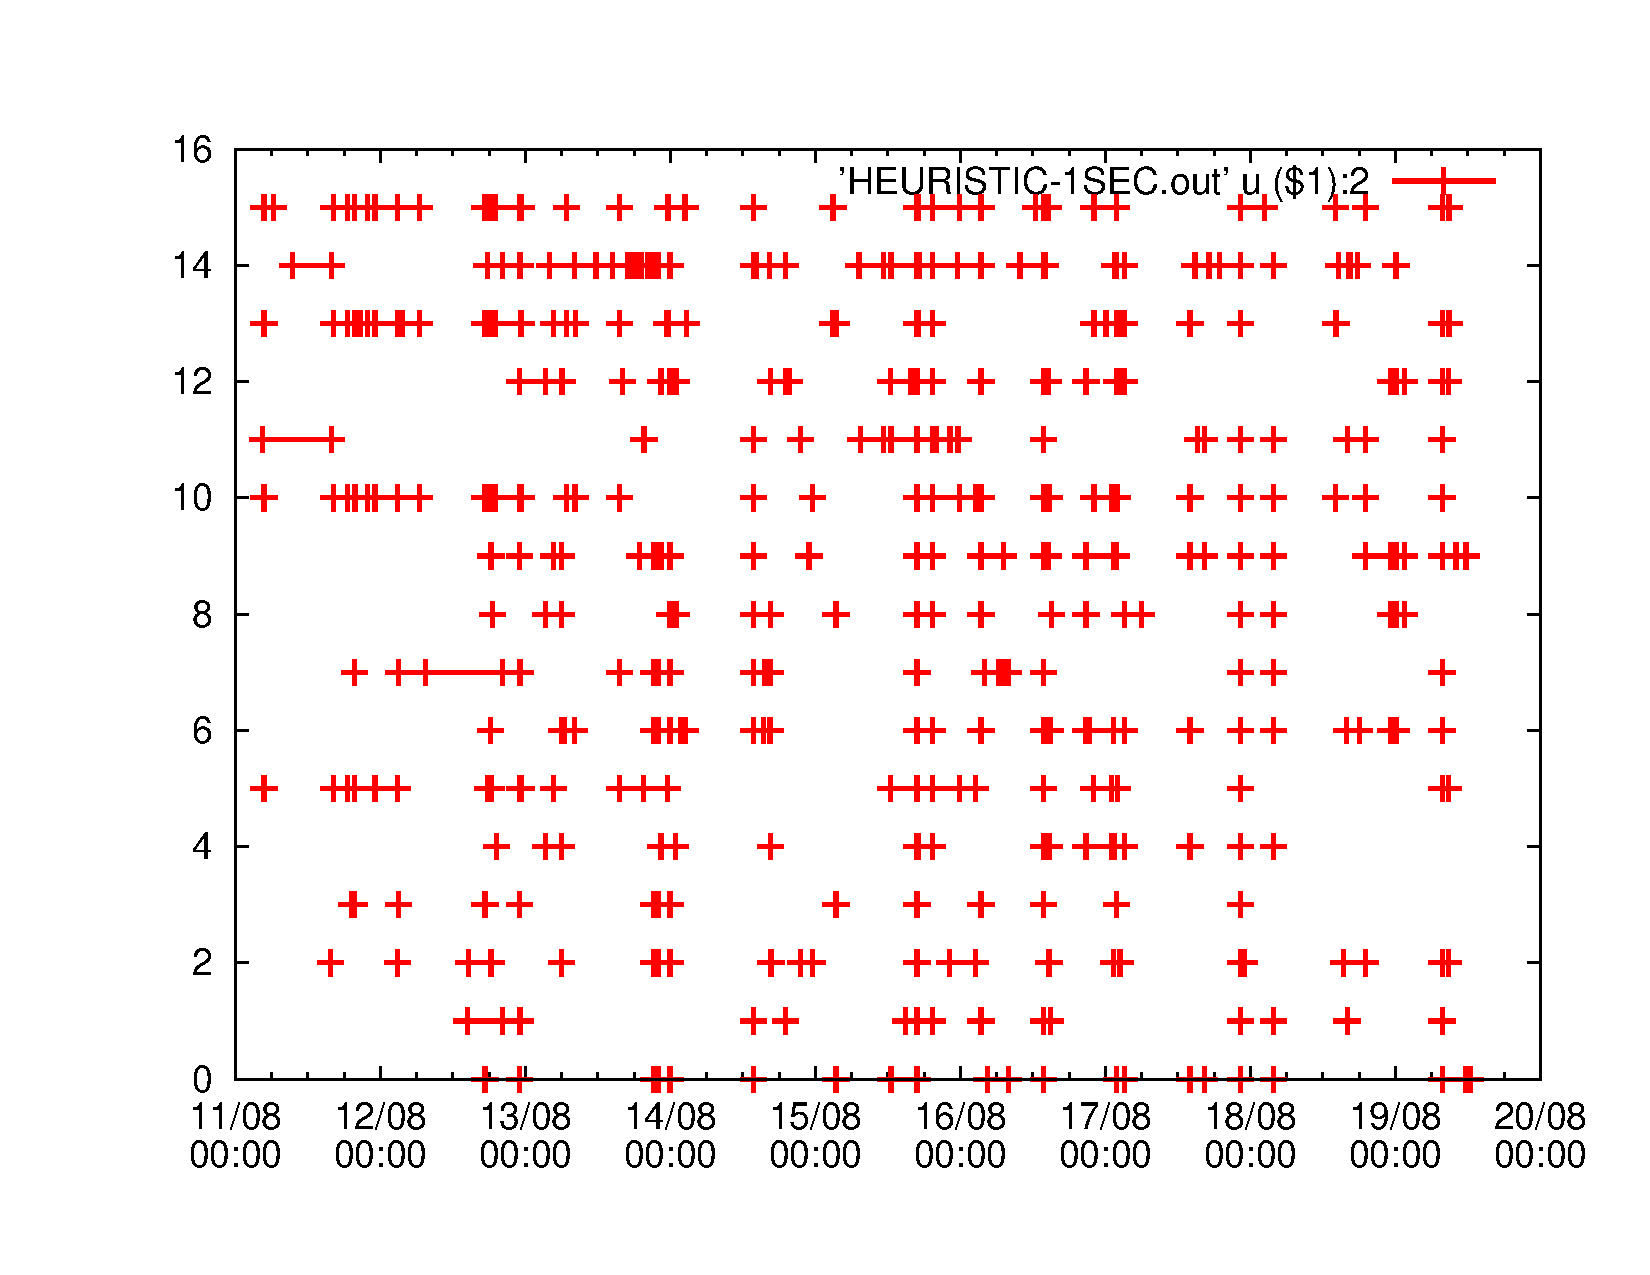
\includegraphics[width=\hsize]{./5-evaluation/figs/timing/TimingHeuristicRuns/HEURISTIC-1SEC.pdf}
%\end{center}
%\caption{\small{\bf Time Location of Consecutive Runs of Timestamps with
%Heuristic Time Difference of Over 1 second}
%{\em \GWAnote{This probably won't be in the paper either.}}}
%\label{fig-heuristic-1sec}
%\end{figure}

%\begin{figure}[t]
%\begin{center}
%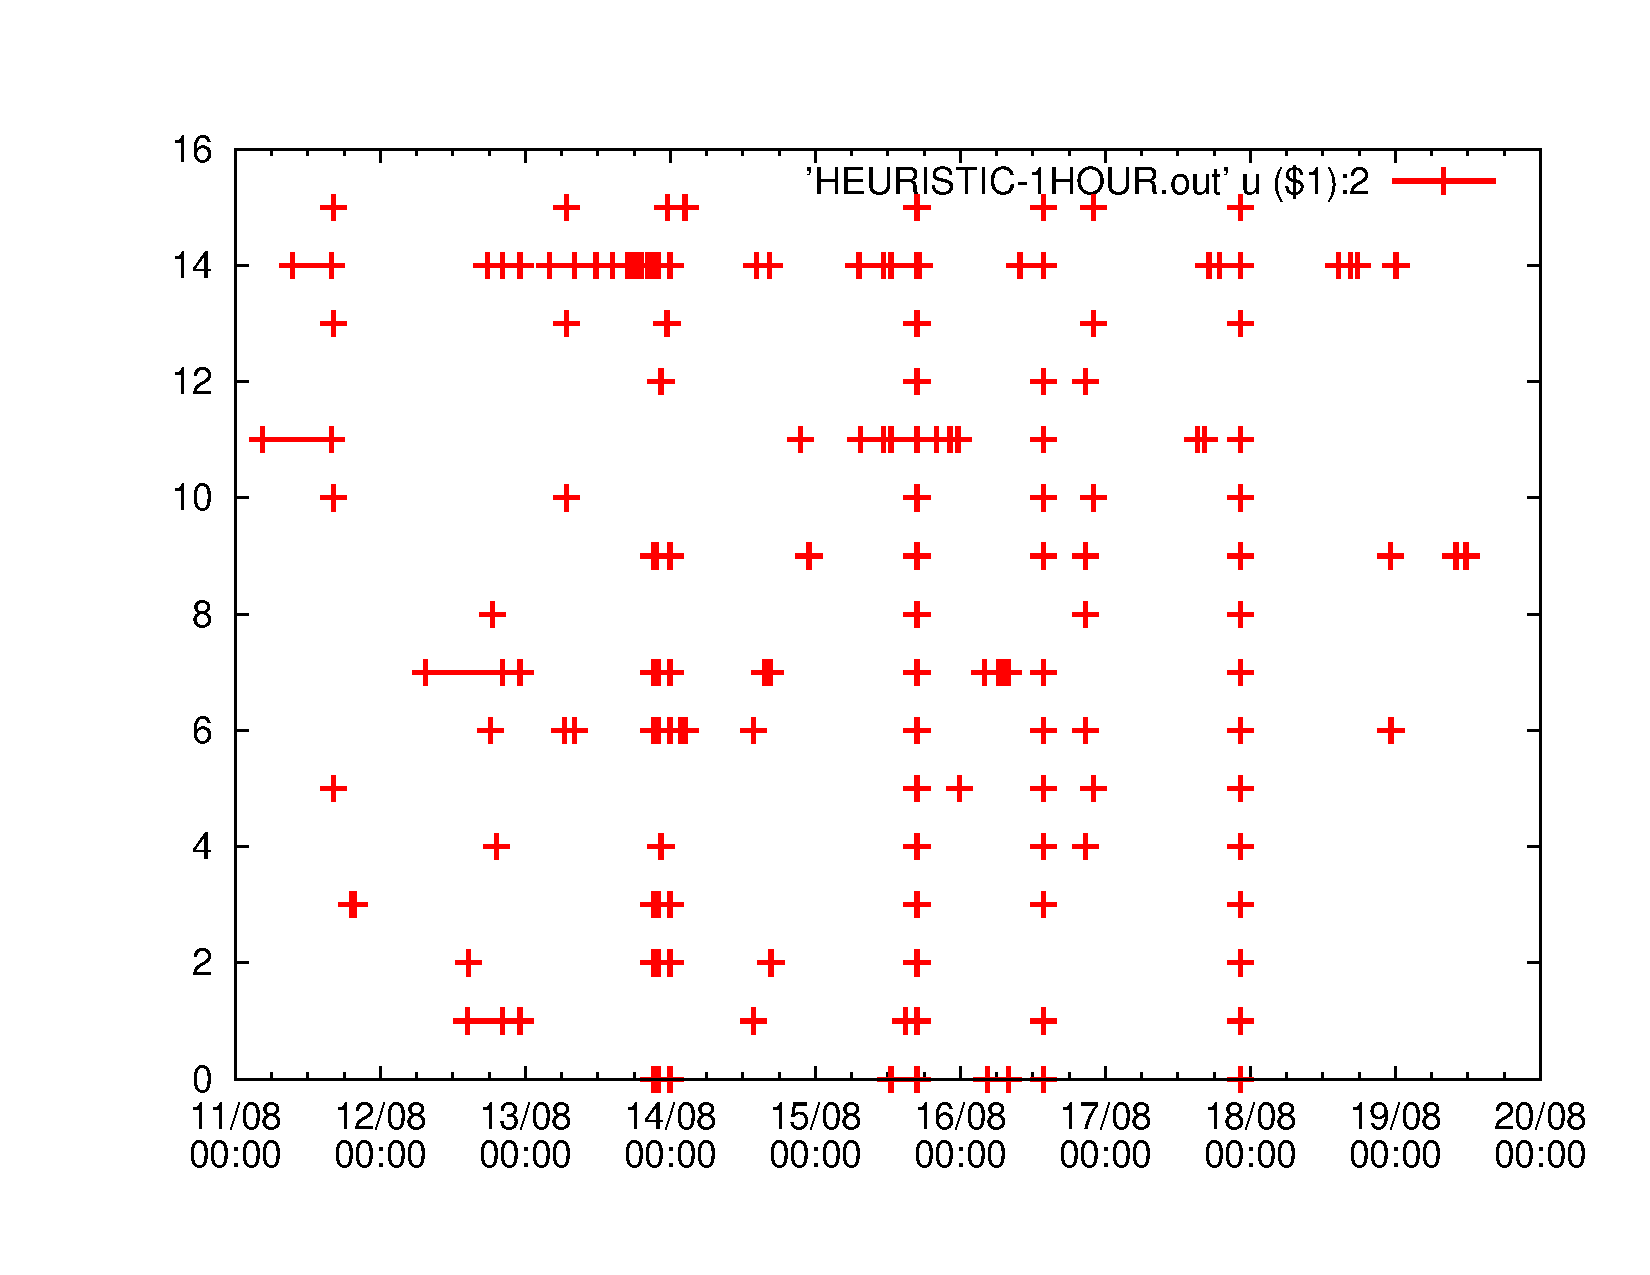
\includegraphics[width=\hsize]{./5-evaluation/figs/timing/TimingHeuristicRuns/HEURISTIC-1HOUR.pdf}
%\end{center}
%\caption{\small{\bf Time Location of Consecutive Runs of Timestamps with
%Heuristic Time Difference of Over 1 hour}
%{\em Marked regions on this time-series indicate periods during with a given
%nodes time data points had a heuristic error of over 1 hour.  There are
%several small, well-correlated periods at periodic intervals caused by clock
%rollover on the root node.  Larger intervals show periods when FTSP errors
%prevented nodes from accurated time stamping data.  As shown in Figure FIXME
%and Figure FIXME this occured more often for certain nodes than for others.
%\GWAnote{I think that if we keep one of these it should be this one.  1 hour
%is obviously a bad heuristic diff and this graph looks a lot like the 60
%second one.}}}
%\label{fig-heuristic-1hour}
%\end{figure}

%\begin{figure}[t]
%\begin{center}
%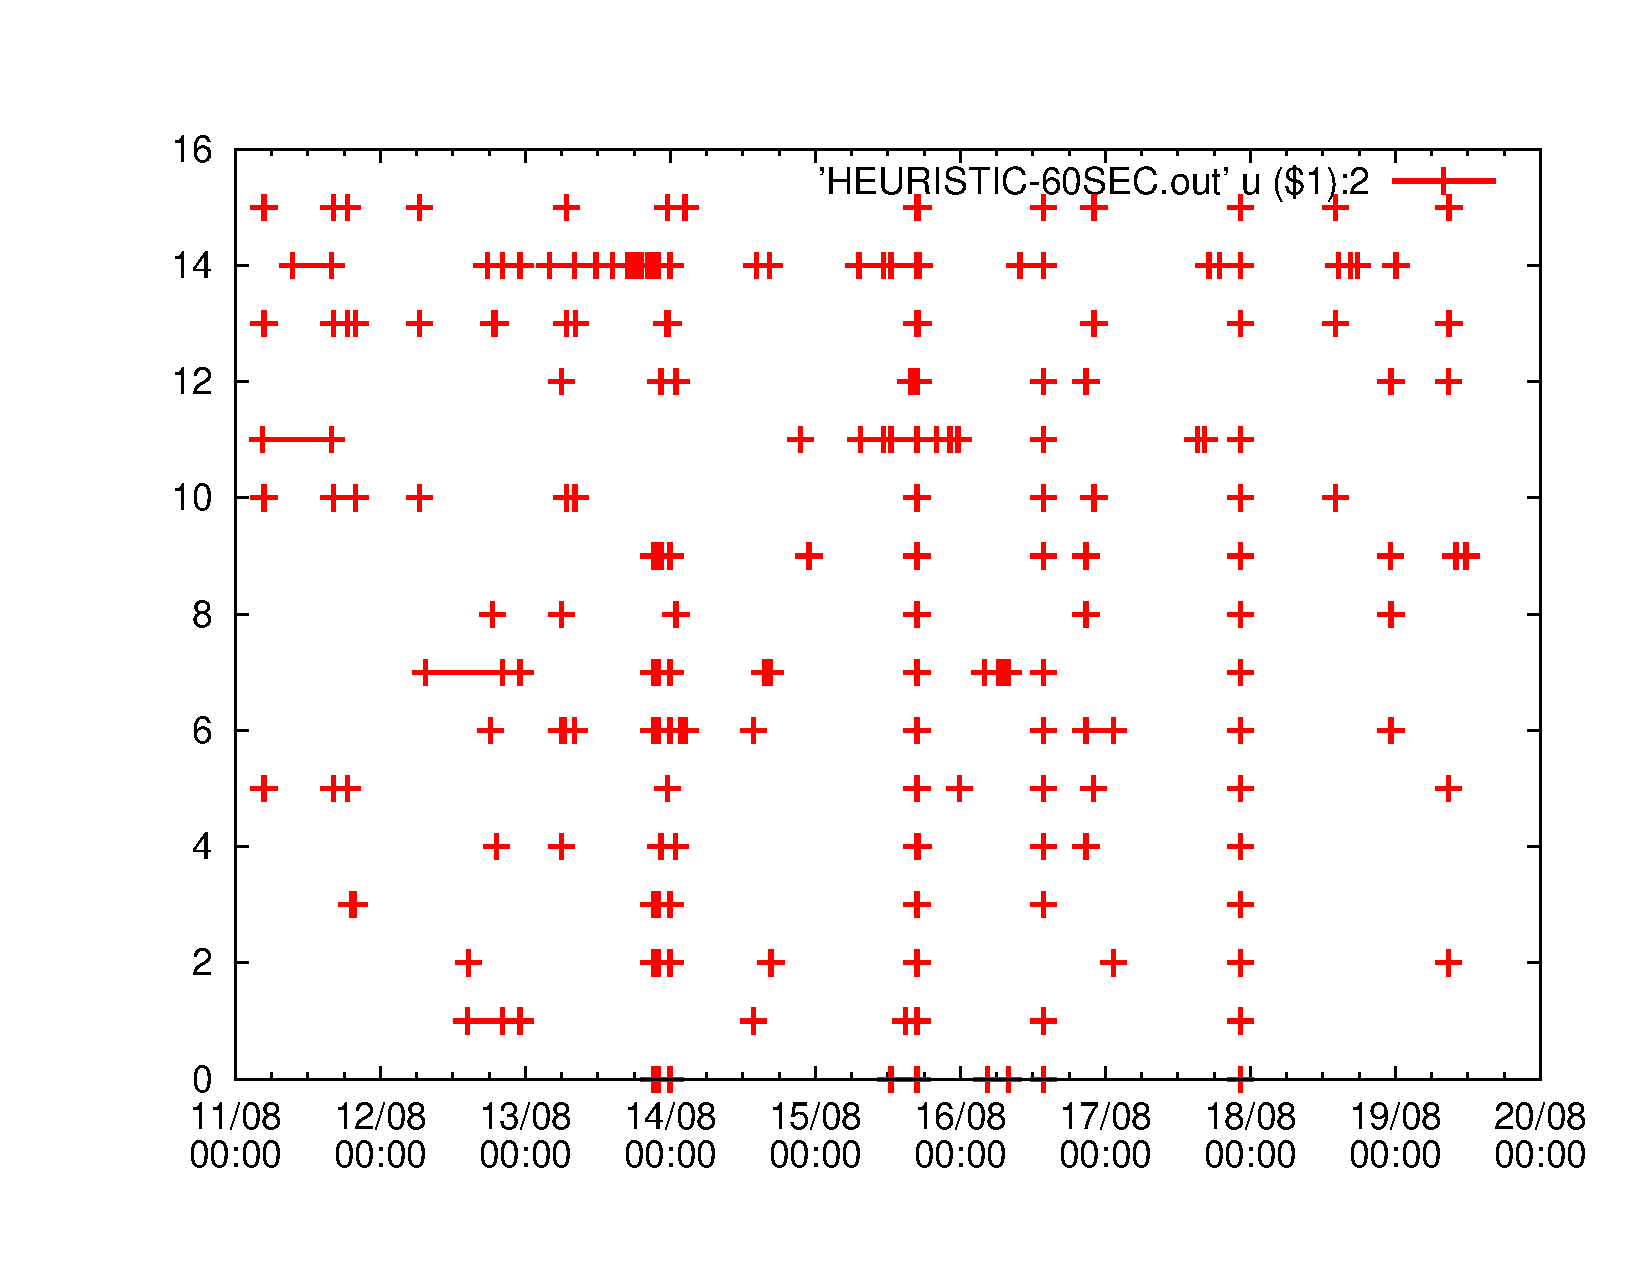
\includegraphics[width=\hsize]{./5-evaluation/figs/timing/TimingHeuristicRuns/HEURISTIC-60SEC.pdf}
%\end{center}
%\caption{\small{\bf Time Location of Consecutive Runs of Timestamps with
%Heuristic Time Difference of Over 60 seconds}
%{\em \GWAnote{Don't think that we need this one either.}}}
%\label{fig-heuristic-60sec}
%\end{figure}

%\begin{figure}[t]
%\begin{center}
%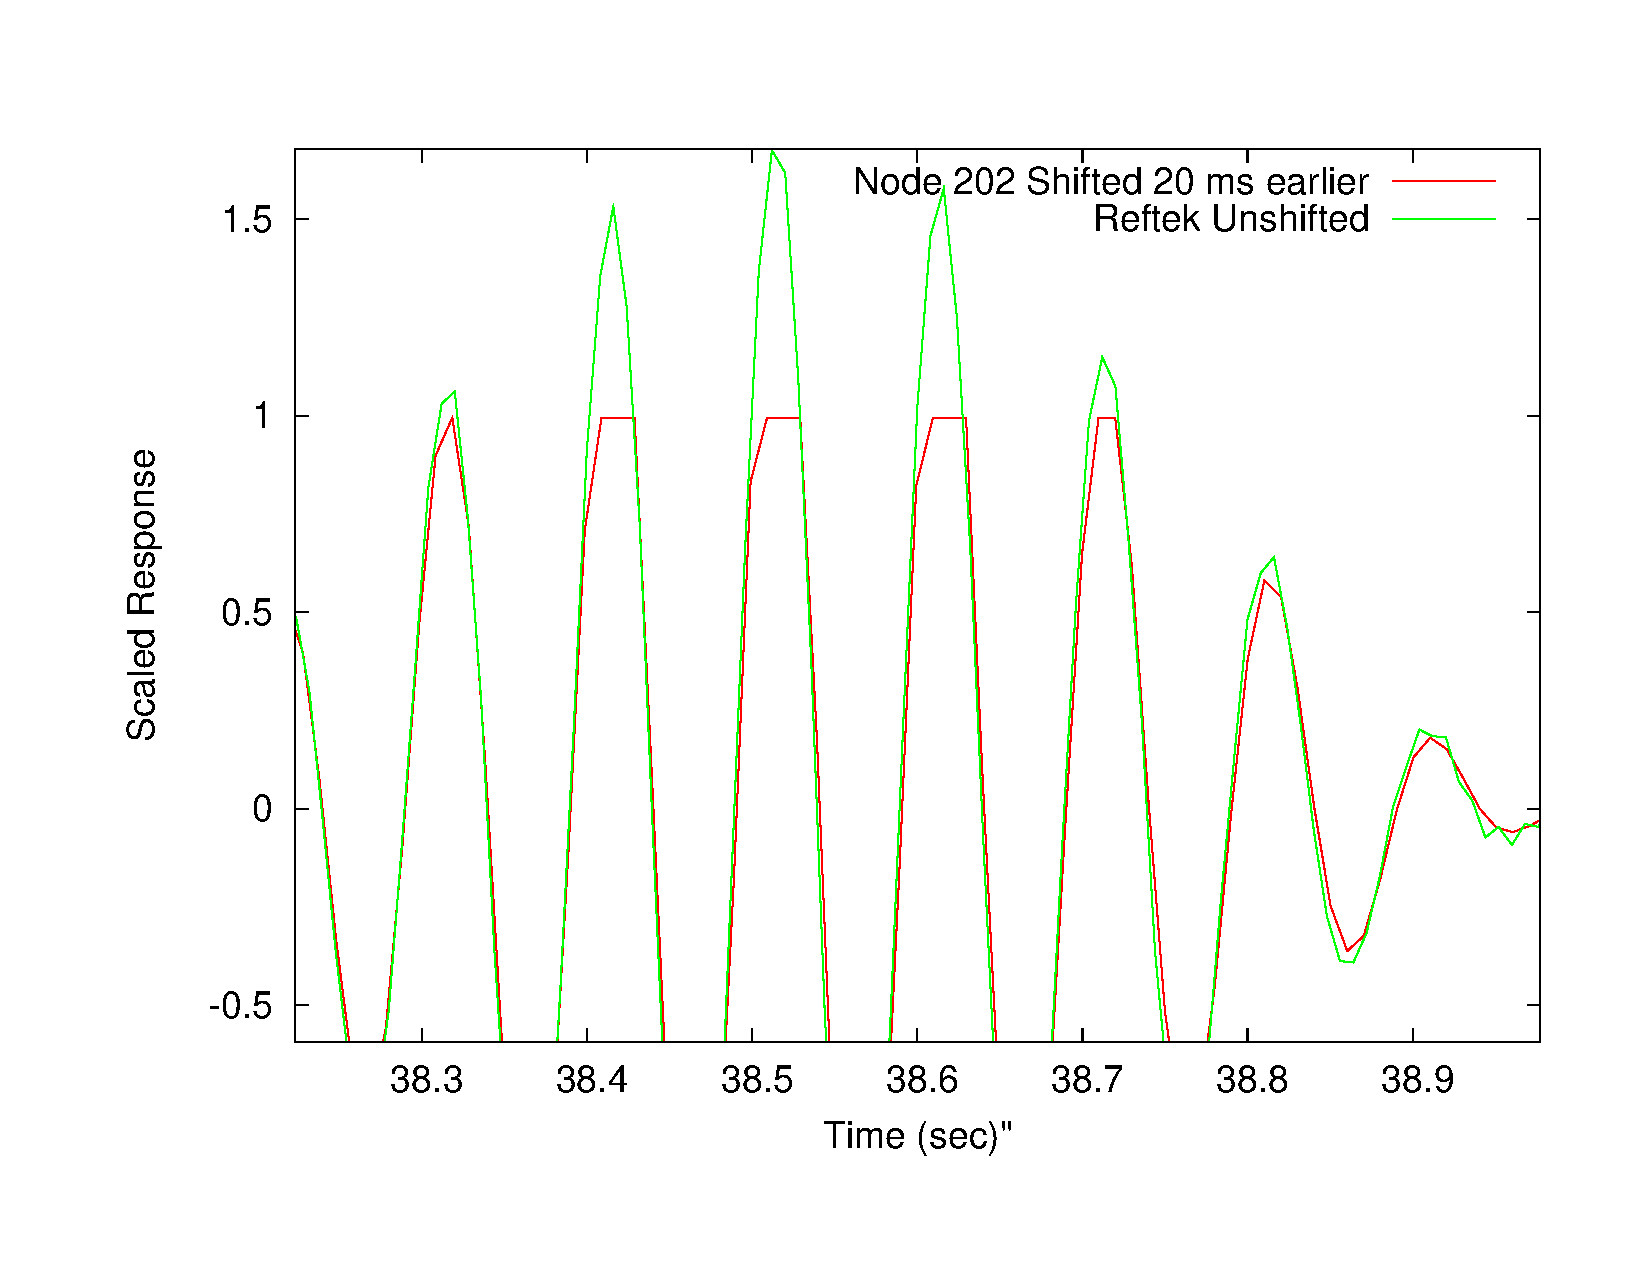
\includegraphics[width=\hsize]{./5-evaluation/figs/timing/FirstReftekComparison/COMPARISON-SHIFTED.pdf}
%\end{center}
%\caption{\small{\bf Reftek Side-by-side Test Signals with 15 ms Shift Applied}
%{\em This graph shows the output of the Reftek side-by-side test (described
%in more detail in Section FIXME) after applying a 15ms time shift as
%suggested by the engineers at Analog Devices.}}
%\label{fig-comparisonshifted}
%\end{figure}

%\begin{figure}[t]
%\begin{center}
%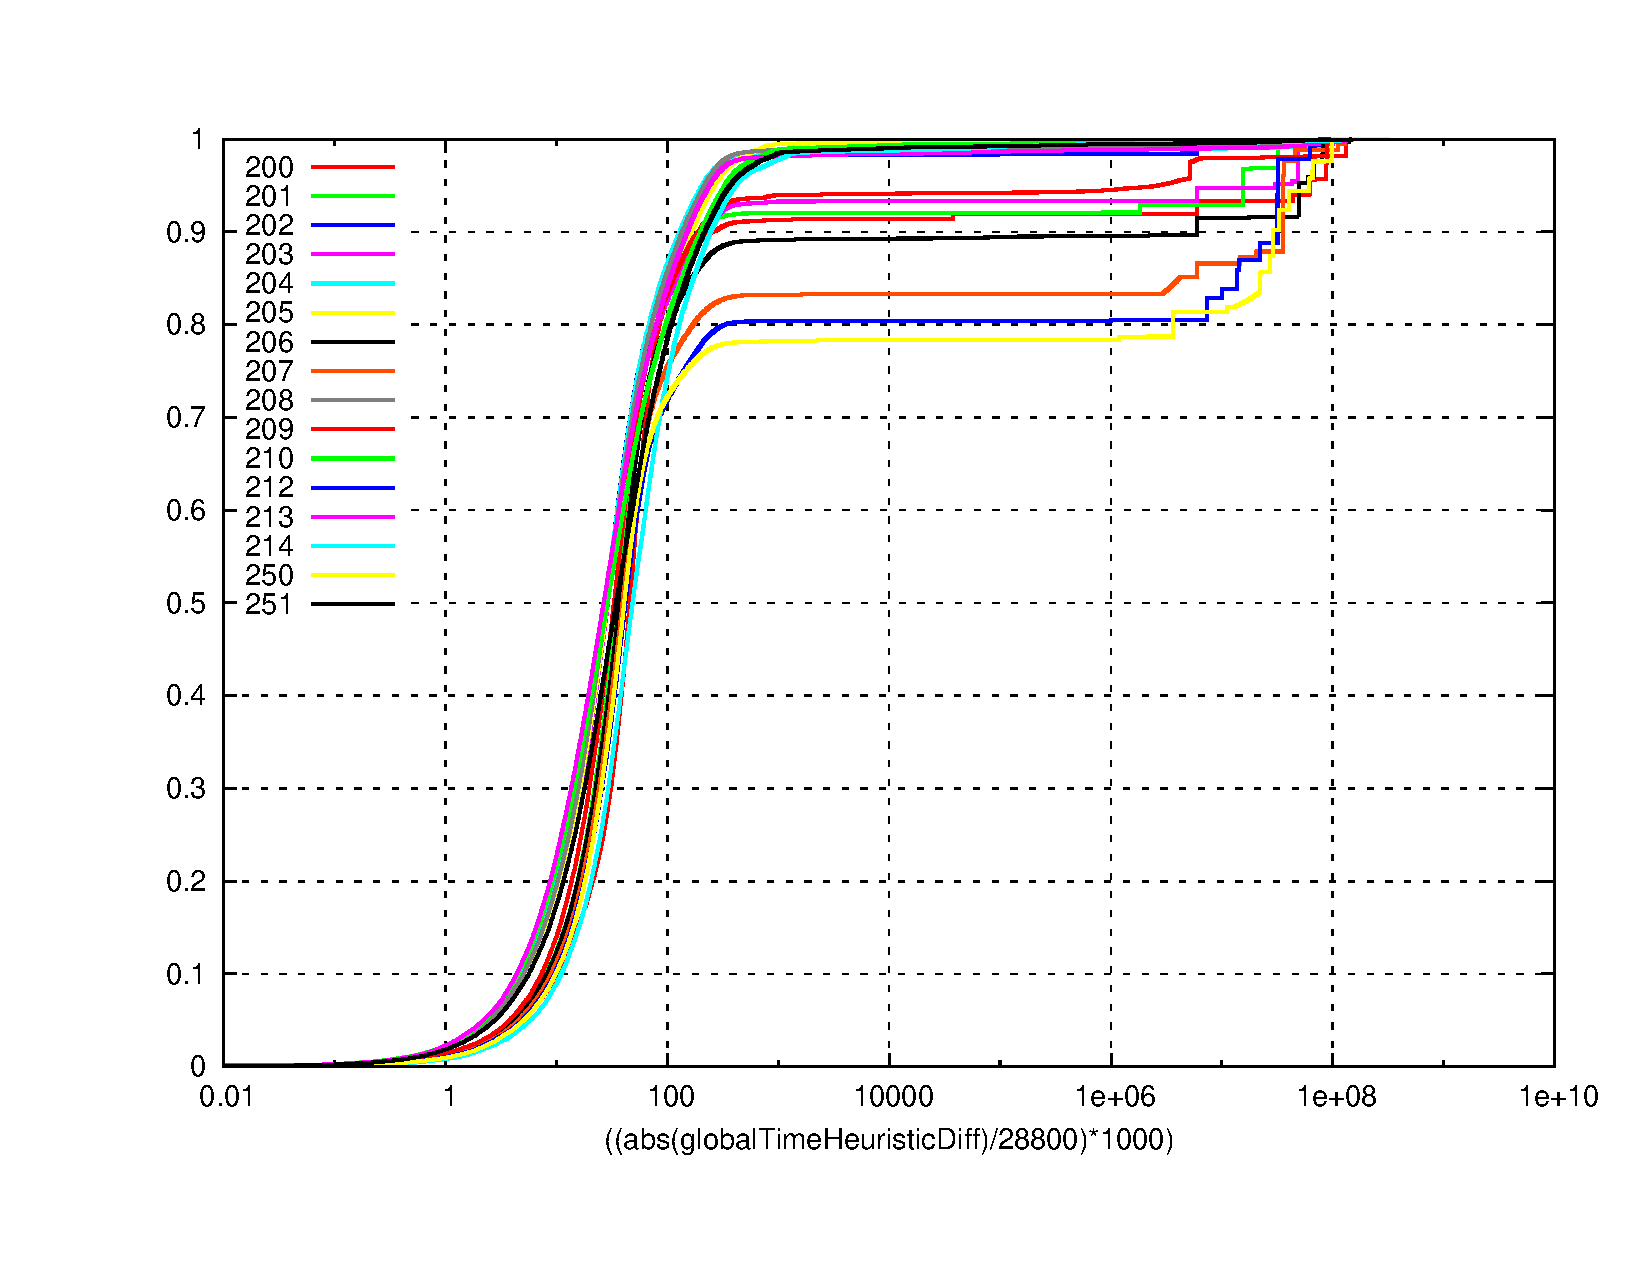
\includegraphics[width=\hsize]{./5-evaluation/figs/timing/TimingHeuristicDiffs/TIMINGHEURISTICABS.pdf}
%\end{center}
%\caption{\small{\bf Distribution of Absolute Heuristic Time Difference by
%Node ID} {\em The graph shows the distribution of absolute heuristic time
%differences (as described in Section~\ref{}).  The time rectification process discards
%points with a difference of over 1000ms (1 sec).}}
%\label{fig-timingheuristicabs}
%\end{figure}

%\begin{figure}[t]
%\begin{center}
%\includegraphics[width=\hsize]{./5-evaluation/figs/timing/SampleRates/SAMPLERATESHISTOGRAM.pdf}
%\end{center}
%\caption{\small{\bf Histogram of Output Sample Rate on Data Records}
%{\em As a first step in the data ground truthing we examined the apparent
%sample rate on each data record that emerged as an output of the time
%rectification process.  Data sampling was driven by an 50 parts-per-million
%oscillator on the interface board independent of the oscillator used for
%FTSP. What this figure shows is that on data records that we were able to
%time rectify the sample rates that emerge conform to the rates we would
%expect from the oscillator on board the interface board. \GWAnote{Not sure we
%need this and maybe it should be a CDF?}}}
%\label{fig-samplerates}
%\end{figure}

%\begin{figure}[t]
%\begin{center}
%\includegraphics[width=\hsize]{./5-evaluation/figs/timing/TelosLabTiming/ABSOLUTEERROR.pdf}
%\end{center}
%\caption{\small{\bf Distribution of Bench Test FTSP Global Time Errors}
%{\em During the experiment described in Section~\ref{} we used periodic
%heartbeat messages to collect synchronous local time, global time pairs
%across the network.  This graph shows the distribution of the errors with
%respect to the ``true'' global time, that is the stamp recorded on the
%broadcast node when it sent the message.  FTSP performed well: FIXME\% of
%global timestamps reported by nodes within FIXME hops of the FTSP root had
%errors of less than FIXME ms. \GWAnote{This graph should probably show
%absolute values. I'm not sure its worth getting into why this shows a bias in
%one direction or the other...}}}
%\label{fig-absoluteerror}
%\end{figure}

%\begin{figure}[t]
%\begin{center}
%\includegraphics[width=\hsize]{./5-evaluation/figs/timing/TelosLabTiming/MAPPEDERROR.pdf}
%\end{center}
%\caption{\small{\bf Distribution of Bench Test Local to Global Time Mapping Error} 
%{\em For the experiment described in Section~\ref{} we simulated the time
%rectification process by using time data points collected in the status
%messages to map local time values onto known good global time values.  This
%graph shows the distribution of the result errors.  As the graph shows
%FIXME\% of local timestamps collected by nodes within FIXME hops of the FTSP
%root could be rectified to within FIXMEms of the true value. \GWAnote{See the
%note on the other figure like this.}}}
%\label{fig-mappederror}
%\end{figure}

%\begin{figure}[t]
%\begin{center}
%\includegraphics[width=\hsize]{./5-evaluation/figs/timing/FirstReftekComparison/COMPARISON-UNSHIFTED.pdf}
%\end{center}
%\caption{\small{\bf Reftek Side-by-side Test Signals Unshifted}
%{\em \GWAnote{I'm not sure we need to show this.  Or maybe we should, and
%talk about how we used this to discover the ``hidden'' 15ms delay?  Might be
%a better story than the shifted graph.}}}
%\label{fig-comparisonunshifted}
%\end{figure}

%\begin{figure}[t]
%\begin{center}
%\includegraphics[width=\hsize]{./5-evaluation/figs/timing/GlobalTimeProblem/GlobalTimeProblem.pdf}
%\end{center}
%\caption{\small{\bf Example of FTSP Instability Observed During Field
%Deployment}
%{\em As describe in Section~\ref{timing-deploymentfailures} FTSP experienced
%periods of instability during our field experiment.  This graph shows an
%example of what we noticed in the field.  The global time value reported by
%two nodes and the GPS node is plotted against the time that the observatory
%laptop received the status message. At first all the lines are on top of each
%other.  However the graph shows that around 0400 GMT Node 212 began reporting
%a global time off by some 30,000 seconds, or over 8 hours. At around 0930 GMT
%Node 250 also began reporting an erroneous global time value. Although they
%both seem to make corrections at around 0100 hours they do not rejoin the GPS
%node until 1600 hours, producing 4.5 hours of global time downtime for Node
%250 and 9.5 for Node 212.  Although the heuristic filtering described in
%Section~\ref{timing-deploymentfailures} can identify and remove these
%timestamps no data collected by nodes during long outages such as this one
%can be correctly timestamped. Note that the absolute value of the global time
%value shown on the Y-axis is meaningless; global time values are mapped onto
%GMT time using techniques described in Section~\ref{section-timerectification}.}}
%\label{fig-globaltimeproblem}
%\end{figure}

%\begin{figure}[t]
%\begin{center}
%\includegraphics[width=\hsize]{./5-evaluation/figs/timing/MDW/rectification/rectify-STEP1.pdf}
%(a)
%\includegraphics[width=\hsize]{./5-evaluation/figs/timing/MDW/rectification/rectify-STEP2.pdf}
%(b)
%\end{center}
%\caption{\small{\bf Operation of the Heuristic Filter}
%{\em The two figures above show the operation of the heuristic filter. Figure
%(a) shows the raw $(localtime,globaltime)$ pairs collected from the node and
%shows that it experiences a period of FTSP instability.  Figure (b) shows
%that errant timestamps have been removed and a mapping between $localtime$
%and $globaltime$ created.}}
%\label{fig-rectificationprocess}
%\end{figure}

%\begin{figure}[t]
%\begin{center}
%\includegraphics[width=\hsize]{./5-evaluation/figs/timing/FTSPUpDown/FTSPDOWN.pdf}
%\end{center}
%\caption{\small{\bf Percentage of timestamps discarded by filtering.}
%{\em Overall, the filter rejected \XXXnote{7.9\% ???} of the time 
%stamps reported by sensor nodes. However, certain nodes, such as
%node~250, had an unusually large number of FTSP failures.}}
%\label{fig-ftspdown}
%\end{figure}


\section{Data Fidelity}
\label{evaluation-sec-fidelity}

The final and most important measure of our network is its ability to provide
scientifically-meaningful data on the volcano's activity. In this section, we
perform an initial analysis of the seismic and acoustic signals from a
seismological perspective, with the goal of validating the accuracy of the
signal quality and timing.

\subsection{Acoustic wave propagation}

The infrasonic (low-frequency acoustic) waves generated by the volcano are
primarily the result of explosive events. 
%% As such, infrasound is a useful complement to seismic monitoring and
%% can be used to differentiate explosions from other kinds of
%% earthquakes.
We start by measuring the velocity of infrasonic waves recorded by our
network, which is more straightforward than seismic analysis for several
reasons.  First, infrasonic waves generate a clear impulse in the microphone
signal, making it easy to determine the time of the wave arrival at each
sensor. In addition, acoustic waves propagate about an order of magnitude
slower than seismic waves (roughly 340~m/s versus 1500-4000~m/s).
%% , and compared to ground-propagating seismic waves, air is a
%% relatively homogenous medium.
We also expect an infrasonic wave to originate at the vent of the volcano,
simplifying the wave velocity calculation.

%% \begin{figure*}[t]
%% \begin{center}
%% \begin{tabular}{cc}
%% \includegraphics[width=0.4\hsize]{./5-evaluation/figs/fidelity/acousticSeismicSketches.pdf}
%% &
%% \includegraphics[width=0.4\hsize]{./5-evaluation/figs/fidelity/acousticSeismicSketches2.pdf}
%% \\
%% {\small\bf (a) Acoustic wave propagation} &
%% {\small\bf (b) Seismic wave propagation} \\
%% \end{tabular}
%% \end{center} 
%% \caption{\small {\bf Computing wave arrivals of seismic and acoustic
%% waves.} {\em These sketches show the propagation of (a) acoustic
%% and (b) seismic waves from the volcano. While acoustic waves emanate
%% from the vent, seismic waves may be generated by explosions from the
%% vent or sources within the volcano.}}
%% \label{fig-acousticSketch}
%% \label{fig-seismicSketch}
%% \end{figure*}

\begin{figure}[t]
\label{evaluation-fig-acousticSketch}
\begin{center}
\includegraphics[width=\hsize]{./5-evaluation/figs/fidelity/acousticSeismicSketches.pdf}
\end{center}
\caption{\textbf{Computing acoustic wave velocity.}
The velocity of the acoustic wave is calculated based on the distance of each
station from the vent, $d_i$, and the arrival time of the wave at each
station, $t_i$.}
\end{figure}

We identified four events in our data set with a clear infrasonic component.
For each event, we hand-picked the arrival time of the wave at each node
using the time-rectified signal.  Figure~\ref{evaluation-fig-acousticArrival}
plots the wave arrival time versus the distance of each node from the vent.
As shown in Figure~\ref{evaluation-fig-acousticSketch}, the velocity of the
wave can be calculated by performing a linear regression on this dataset.

\begin{figure}[t]
\label{evaluation-fig-acousticArrival}
\begin{center}
\includegraphics[width=\hsize]{./5-evaluation/figs/fidelity/acousticArrival/acoustic.pdf}
\end{center}
\caption{\textbf{Acoustic wave arrival times and velocity.}
This figure shows the acoustic wave arrival time vs. distance from the vent
for 4~separate events. Also shown is the resulting acoustic wave velocity and
the $R^2$ coefficient of determination.}
\end{figure}

The result of this calculation is also shown in
Figure~\ref{evaluation-fig-acousticArrival}.  The velocity of sound in air is
temperature-dependent; for temperatures between 10--20 $^{\circ}$C the
velocity range is 337--343~m/s.  The calculated wave velocities are mostly in
this range, with a mean of 339.5~m/s. The coefficients of determination $R^2$
are very high, between 0.9988~and~0.9999, showing that the timing and quality
of the acoustic data closely matches our expectation of the infrasonic waves
produced by the volcano.

%\begin{figure}[t]
%  \begin{small}
%    \begin{center}
%      \begin{tabular}{|ccc|} \hline
%               {\bf Event} & {\bf Velocity m/s)} & {\bf $R^2$} \\ \hline
%               08/12/05 02:15:18 & 331 & 0.9988 \\
%               08/13/05 01:27:46 & 339 & 0.9998 \\
%               08/15/05 19:29:08 & 346 & 0.9995 \\
%               08/16/05 09:45:14 & 342 & 0.9999 \\ \hline
%               {\bf Mean} & 339.5 & 0.9995 \\
%               {\bf StdDev} & 6.35 & 0.0005 \\ \hline
%      \end{tabular}
%    \end{center}
%  \end{small}
%  \caption{\small{\bf Acoustic time of arrival summary.}  {\em This
%          table summarizes the acoustic wave velocity and $R^2$ from
%          our linear regression.  The mean velocity for the 4 events
%          is 339.5~$m/s$ which is between the expected velocity of
%          soundm, 337~$m/s$ at 10\textcelsius $ $ and 343~$m/s$ at
%          20\textcelsius. The $R^2$ coefficient is very close to 1.0,
%          indicating a very strong correlation.}}
%  \label{fig-acousticArrivalReg}
%\end{figure}

\subsection{Seismic wave propagation}

Analyzing the seismic waves captured by our network is significantly more
challenging. This is primarily because the source locations of seismic waves
are unknown.  Seismic events may originate at the vent (in the case of an
explosion) or deep within the edifice, producing very different patterns of
P-~and S-wave arrivals at each node. A full seismological analysis of our
data is beyond the scope of this paper. However, we present a high-level
measure of the {\em consistency} of the signals captured by our network: that
is, we evaluate whether the seismic wave arrivals are consistent with
expected volcanic activity.

%% Our sensor array was established in a radial geometry for two primary
%% reasons: (1) to understand the attenuation structure of volcanic
%% explosion earthquakes, and (2) to calculate the seismic wavefield
%% incidence for events occurring near the volcanic conduit. Seismic
%% wavefield incidence is an especially important parameter to recover
%% because it provides us with information about the relative depth of
%% volcanic earthquakes. In addition, knowing the velocity structure of the volcanic edifice 
%% provides important geophysical constraints that are used to assess
%% earthquake source parameters.

%% Our sensor array was established in a radial geometry for two 
%% primary reasons: (1) to understand the attenuation structure of 
%% volcanic explosion earthquakes, and (2) to calculate the seismic 
%% wavefield incidence for events occurring near the volcanic
%% conduit.  
%% %Both seismic attenuation, which is the study of how seismic
%% %ground shaking decreases with propagation distance and frequency
%% %content, and wavefield analyses are the focus of ongoing study with
%% %the collected dataset.
%% Seismic wavefield incidence is an especially important parameter to
%% recover because it provides us with information about the relative
%% depth of volcanic earthquakes.  
%For a simplified 2-D geometry, the apparent velocity $V_a$ of seismic
%wave arrivals across the array is determined by the intrinsic 
%P-wave velocity $V_p$ of the medium and angle of incidence $\theta$ 
%of seismic energy on the array: $V_a = V_p / \cos(\theta)$.  
%Typically depth is hard
%to determine through traditional means because seismic stations at
%volcanoes are most easily deployed around the periphery of the volcano
%(providing good epicentral locations but poor depth constraints).  
%
%Our sensors were deployed along a radial trajectory away
%from the vent in order to calculate the move-out of first arrivals
%(i.e., time distribution of compressional P-Wave first arrivals).
%This allows us to discriminate sources originating in the shallow
%portion of the cone near the vent from events occurring more deeply.
%Furthermore, variations in apparent velocity, calculated from the
%move-out, enable us to estimate origin depth of various events.
%
%For a near-surface source in the vicinity of the
%vent, $\theta$ approaches zero and apparent velocity approaches intrinsic
%compressional velocity of the medium.  Conversely, for a deeper source
%(i.e., volcano-tectonic event), seismic angles can steeply impinge
%upon the free surface of the volcanic edifice leading to infinite
%apparent velocity.  For both types of events presented in Figure 3, the
%lowest apparent velocities (1.5 to 2.0 km/s) is observed towards the
%far end of the array (Figure 3).  This is the value that most closely
%approximates the seismic P-wave velocity of the volcano in this locale.
%% In addition, knowing the velocity structure of the volcanic edifice 
%% provides important geophysical constraints that are used to assess earthquake
%% source parameters.

\begin{figure}[t]
\label{evaluation-fig-seismicArrivalScatteredNode}
\begin{center}
\includegraphics[width=\hsize]{./5-evaluation/figs/fidelity/seismicArrival/arrivalTimesPlotScatteredNode.pdf}
\end{center}
\caption{\textbf{Time of arrival of each node over multiple events.}
This graph shows the spread of arrival times for each node.  The arrival time
and distance is relative to node~207.  The arrival time for each node is
fairly consistent over multiple events, with the exception of node~214.  The
shaded area indicates a move-out velocity of less than 1,500 $m/s$.}
\end{figure}

The most natural measure of data consistency is whether the time of the
seismic P-wave arrival at each sensor falls within an expected {\em envelope}
based on the minimum speed at which seismic waves are believed to propagate
at Reventador, which we estimate as 1500~m/s. We took 15~seismic events with
clear P-wave arrivals and used an automatic algorithm~\cite{pwave-picking} to
determine the wave arrival time.\footnote{Unlike acoustic waves, determining
seismic wave arrival times is notoriously difficult. The seismograms in
Figures~\ref{evaluation-fig-jjExplosion} and
Figure~\ref{evaluation-fig-jjTectonic} should give the reader some
appreciation for this.} 

Figure~\ref{evaluation-fig-seismicArrivalScatteredNode} shows a scatterplot
of the arrival times with respect to node~207, which was chosen as an
arbitrary reference point since data for this node appeared in all 15~events.
The $y$-axis represents the distance of each node from~207. Depending on the
seismic source location, we expect waves to arrive both before and after
node~207.  However, the slowest wave speed (1500~m/s) dictates the maximum
difference in the wave arrival between each station.\footnote{Note that there
is no lower bound on arrival times, since a wave emanating from a deep source
could arrive at all stations nearly simultaneously.} The shaded area in
Figure~\ref{evaluation-fig-seismicArrivalScatteredNode} covers the
``exclusion envelope'' of arrival times at each station.  As the figure
shows, only 2~out of~124 arrivals fall outside of this envelope.

%It is interesting to note that although node~204 is closest
%to the vent, seismic waves do not appear to reach this node first;
%this suggests a deep source under the middle of the sensor array,
%which is by itself an interesting scientific finding.

%The automated picking algorithm uses a tiered approach.  Seismograms
%are initially prepared by extracting the envelope waveform using the
%Hilbert transform.  This is followed by a median smoothing filter to
%remove noise glitches and otherwise undesirable high frequency
%signals.  The smoothed envelopes are then passed through a series of
%gradually refined forward-backward (sometimes called STA/LTA)
%root-mean-square ratio estimate.  Arrival times where significant
%changes in the ratio curves occur are saved.  Several thresholds are
%examined statistically and the initial estimate of the pick is
%determined by robust quantile cut-offs.
%
%This initial arrival time estimate is then used as a first guess
%provided to the so-called ARAIC algorithm (Auto-Regressive Akaiki
%Information Criterion) of Sleeman and van Eck~\cite{pwave-picking}.
%The ARAIC method uses an autoregressive characterization of the noise
%and signal and finds the time along the trace that minimizes the
%maximum likelihood function fit to the AR models.  The algorithms were
%implemented in R~\cite{r-book}, an interactive computation platform.

\begin{figure}[t]
\label{evaluation-fig-jjExplosion}
\begin{center}
\includegraphics[width=\hsize]{./5-evaluation/figs/fidelity/seismicArrival/johnson/2005-08-16_09-45-14.pdf}
\end{center}
\caption{\textbf{Explosion earthquake event at 08/16/2005 09:45:14 GMT.}
P-wave arrivals have been identified manually and a second-order polynomial
(solid line) is fit to the arrivals. The arrival time move-outs are
consistent with a shallow near-vent source.}
\end{figure}

Finally, we take a closer look at two seismic events recorded by our array.
Figures~\ref{evaluation-fig-jjExplosion}~and~\ref{evaluation-fig-jjTectonic}
show seismograms from each of the sensor nodes after time rectification.  The
$y$-axis corresponds to the distance of each node from the vent.  For each
event, the P-wave arrivals have been determined by hand and a second-order
polynomial has been fit to the arrival times at each node for clarity.

These two events show a very different pattern of wave arrival times.
Figure~\ref{evaluation-fig-jjExplosion} shows the seismic wave arriving first
at stations near the vent (nodes~204 and 213). This is consistent with a
shallow near-vent source corresponding to an explosion. This is confirmed by
the corresponding acoustic data (shown in
Figure~\ref{evaluation-fig-acousticArrival}) attributed to explosive
expansion of gas. 

In contrast, Figure~\ref{evaluation-fig-jjTectonic} shows an event with the
earliest arrivals in the middle of the sensor array and the endpoints
relatively delayed; many such events were recorded by our network.  This
distribution implies a deeper source.  At the same time, seismic velocity in
the uppermost cone, which is comprised of unconsolidated volcanic deposits,
is presumed to be slower.  Such volcano-tectonic events are likely generated
by the fracturing of solid media typically induced by pressurization within
the edifice. This preliminary study demonstrates the value of our wireless
sensor network for collecting accurate signals that can be subjected to
seismological analysis.

\begin{figure}[t]
\label{evaluation-fig-jjTectonic}
\begin{center}
\includegraphics[width=\hsize]{./5-evaluation/figs/fidelity/seismicArrival/johnson/2005-08-15_16-04-37.pdf}
\end{center}
\caption{\textbf{Tectonic earthquake event at 08/15/2005 16:04:37 GMT.}
In this event, seismic waves are first recorded near the middle of the sensor
array. This is due either to a source closer to the center of the array,
variations in velocity structure, or most likely both.}
\end{figure}


%%%%%%%%%%%%% OLD text %%%%%%%%%%%%%%%%%%%%%%%%
% - How different from acoustic
% - Subset of events that we analyzed
% - How we did linear fit and table fo results

%% \begin{figure}[t]
%% \begin{center}
%% \includegraphics[width=\hsize]{./5-evaluation/figs/fidelity/seismicArrival/arrivalTimesPlot.pdf}
%% \end{center}
%% \caption{\small{\bf Time of arrival for the seismic data.}
%% {\em This figure shows the seismic wave arrival time offset by the
%% first arrival vs. normalized distance between nodes.  The graph indicates that
%% most events originate closer to the center of the array.}}
%% \label{fig-seismicArrival}
%% \end{figure}

%% \begin{figure}[t]
%% \begin{center}
%% \includegraphics[width=\hsize]{./5-evaluation/figs/fidelity/seismicArrival/arrivalTimesPlotFit.pdf}
%% \end{center}
%% \caption{\small{\bf Liner regression for the time of arrival for the seismic data.}
%% {\em This arrival times of nodes to the right of the node with
%% the first arrival are mirrored about the x-axis.  This allows us to
%% draw a linear fit through the data points.  As we can see, most events
%% have a similar slope which indicates consistent wave velocities.}}
%% \label{fig-seismicArrivalFit}
%% \end{figure}

%% \begin{figure}[t]
%% \begin{center}
%% \includegraphics[width=\hsize]{./5-evaluation/figs/fidelity/seismicArrival/arrivalTimesPlotFit.pdf}
%% \end{center}
%% \caption{\small{\bf Liner regression for the time of arrival for the seismic data.}
%% {\em This arrival times of nodes to the right of the node with
%% the first arrival are mirrored about the x-axis.  This allows us to
%% draw a linear fit through the data points.  As we can see, most events
%% have a similar slope which indicates consistent wave velocities.}}
%% \label{fig-seismicArrivalFit}
%% \end{figure}

%% \begin{figure}[t]
%% %  \begin{minipage}[t]{.45\textwidth}
%%   \begin{small}
%%     \begin{center}
%%       \begin{tabular}{|ccc|} \hline
%%                {\bf Event} & {\bf Velocity (m/s)} & {\bf $R^2$} \\ \hline
%%                2005-08-11\_08.33.49 & 2356.97 & 0.91 \\
%%                2005-08-11\_09.12.38 & 5519.13 & 0.89 \\
%%                2005-08-11\_15.04.27 & 4287.73 & 0.99 \\
%%                2005-08-12\_00.30.40 & 1324.12 & 0.96 \\
%%                2005-08-12\_02.15.18 &  832.95 & 0.93 \\
%%                2005-08-13\_02.17.32 & 3376.40 & 0.96 \\
%%                2005-08-13\_04.24.42 & 2406.30 & 0.94 \\
%%                2005-08-13\_07.08.05 & 3241.98 & 0.95 \\
%%                2005-08-14\_04.32.29 & 8204.96 & 0.67 \\
%%                2005-08-14\_20.17.02 & 3061.23 & 0.87 \\
%%                2005-08-15\_09.11.28 & 3175.71 & 0.89 \\
%%                2005-08-15\_16.04.37 & 2903.11 & 0.51 \\
%%                2005-08-16\_01.32.19 & 2173.40 & 0.65 \\
%%                2005-08-16\_18.30.04 & 2981.71 & 0.77 \\
%%                2005-08-18\_02.45.51 & 3621.04 & 0.81 \\ \hline
%%       \end{tabular}
%%     \end{center}
%%   \end{small}
%%   \caption{\small{\bf Coefficient of determination ($R^{2}$) for events.}
%%           {\em The coefficien of determination is a measure of how well the
%%           regression line represents the data.  A coefficient value greater than
%%           0.65 is generally described as a strong correlation.  As we can see,
%%           most of our events have a coorelation higher than 0.65 indicating a good fit.}}
%%   \label{fig-seismicArrivalReg}
%% %  \end{minipage}
%% \end{figure}


%% \begin{figure}[t]
%% \begin{center}
%% \includegraphics[width=\hsize]{./5-evaluation/figs/fidelity/seismicArrival/arrivalTimesPlotReg.pdf}
%% \end{center}
%% \caption{\small{\bf Coefficient of determination ($R^{2}$) for events.}
%% {\em The coefficien of determination is a measure of how well the
%% regression line represents the data.  A coefficient value greater than
%% 0.65 is generally described as a strong correlation.  As we can see,
%% most of our events have a coorelation higher than 0.65 indicating a good fit.}}
%% \label{fig-seismicArrivalReg}
%% \end{figure}


%% \begin{figure}[t]
%% \begin{center}
%% \includegraphics[width=\hsize]{./5-evaluation/figs/fidelity/seismicArrival/arrivalTimesPlotScatteredEvent.pdf}
%% \end{center}
%% \caption{\small{\bf Time of arrival of nodes for each event.}
%% {\em This graph shows the spread of arrival times.  The arrival times
%% are relative to node 207.  As we can see, most arrival times are
%% within a 1 second window of each other with a few outliers.}}
%% \label{fig-seismicArrivalScatteredEvents}
%% \end{figure}

%\begin{figure}[t]
%\begin{center}
%\includegraphics[width=0.8\hsize,angle=90]{./5-evaluation/figs/timing/RV213/2005-08-15_16.04.37/213VREFTEK-NO-OFFSET.pdf}
%(a)
%\includegraphics[width=0.8\hsize,angle=90]{./5-evaluation/figs/timing/RV213/2005-08-15_16.04.37/213VREFTEK-POSITIVE48MS-OFFSET.pdf}
%(b)
%\end{center}
%\caption{\small{\bf Comparison of Node 213 and Reftek Signals}
%{\em The figures above show two signals, one collected by a sensor
%network station, Node 213, the other collected by a Reftek data logger
%attached to a broadband seismometer. Figure (a) shows the signals before a
%shift is applied, and Figure (b) shows the signals with a 48 ms shift
%applied. Both signals have been bandpass filtered between 6 and 8 Hz to
%reduce the differences in instrument response.  As these figures show a 48 ms
%shift produces a good match at the arrival time of the energy.  The
%signals are expected to differ throughout the coda showing the arrival of
%S-waves. \GWAnote{Need a better way to describe this...}}}
%\label{fig-rvenv213}
%\end{figure}



\chapter{Addressing Data Quality with Lance}
\label{chapter-lance}

One of the core challenges that emerges in high data-rate networks is the
inability of the network to reliable collect all sampled data. This can be
either due to bandwidth constraints --- when data is being sampled faster
than it can be retrieved --- or to energy constraints that emerge when
duty-cycling sensor node radios in order to save power and meet a target
lifetime.

A typical approach to addressing this challenge is to try and prioritize
certain signals over others. However, many times these resource-management
decisions are made in \textit{ad hoc} or application-specific ways, limiting
the applicability and hurting the performance of solutions that attempt to
bridge multiple application domains.

Optimizing reliable data acquisition requires a coordinated approach to
managing both limited energy capacity and severely constrained radio
bandwidth. Depending on the sampling rate and resolution, downloading signals
may take longer than real time: while low-power sensor node radios obtain
single-hop throughput of about 100~kBps, the the best reliable protocols
achieve less than 8~kBps for a single transfer over multiple
hops~\cite{flush-sensys07}. Likewise, to achieve long lifetimes in the field,
the energy cost of downloading a signal from the network must be carefully
considered. The fundamental challenge is how to best direct these limited
network resources to acquire the most valuable data to the application.

This chapter describes \textit{Lance}, a general approach to bandwidth and
energy management for reliable signal collection in wireless sensor networks.
In Lance, each node acquires data at potentially high rates. For each
application data unit (ADU), each node generates a concise ADU
\textit{summary}, which is periodically sent to the base station and used to
compute an ADU \textit{value}. Lance computes an ADU \textit{download
schedule} based on these values and uses a reliable transfer protocol to
download ADUs according to this schedule.

Energy usage and battery lifetime are major concerns for long-term sensor
network deployments. Lance incorporates a \textit{cost estimator} that
predicts the energy cost for reliably downloading each ADU from the network.
We describe a novel energy cost estimation algorithm that uses information on
the network topology to determine the energy cost at the sensor node hosting
the ADU as well as intermediate nodes affected by the multihop transfer
protocol. Information from the cost estimator is used to adjust the download
schedule for ADUs, allowing Lance to target a battery lifetime for the
network by load-balancing download operations in a manner that adheres to an
energy schedule.

Lance incorporates a general framework for managing bandwidth and energy that
decouples the mechanism for prioritizing resource allocation from the
application-specific policies used to assign ADU values. This is accomplished
through user-supplied \textit{policy modules} that permit a range of
sophisticated prioritization policies to be tailored for specific
applications. Policy modules allow Lance to target a broad range of
optimization metrics, including node-local and network-wide value
maximization, lifetime targeting, and acquiring temporally- or
spatially-correlated data from across the network. Policy modules allow the
network's behavior to be significantly altered at the base station, without
reprogramming the sensor nodes themselves.

Lance emerged as a direct result of our field experiences at Reventador
volcano in 2005. We were frustrated by our network's inability to collect all
sampled data, and, given it's relatively modest size (16~nodes), we
anticipated this problem impeding future efforts to deploy large scientific
macroscopes. Our 2005 volcano monitoring system strove to identify and
acquire the most ``interesting'' signals --- such as earthquakes and
explosions --- and thereby avoid wasting resources on ``uninteresting''
signals. However, like other approaches ours was too tailored to our target
application and too embedded in application-specific code.

We saw an opportunity for an architectural solution to coordinated resource
management that would optimize the application-specific value of the data
acquired. Such an architecture would both improve the performance of our
volcano-monitoring macroscope while benefiting other high data-rate
applications. We have been able to validate the performance of Lance and
demonstrate its utility both to our volcano-monitoring application and to a
body sensor network designed to monitor patients with neuromuscular disease.

This chapter is structured as follows:

\begin{enumerate}

\item We motivate the Lance architecture and describe its goal in more detail
in Section~\ref{lance-sec-motivation}.

\item Section~\ref{lance-sec-architecture} presents the Lance architecture in
detail, which is the first system to provide a value-driven bandwidth and
energy management framework for high-data-rate sensor networks.

\item In Section~\ref{lance-sec-policies} we describe Lance's policy modules,
which offer a clean separation of policy and mechanism that allows the system
to be tailored to a broad range of applications.

\item Section~\ref{lance-sec-adaptation} discusses the process of adapting
our volcano-monitoring system to the Lance architecture and also points out
other applications that are a good fit for this approach.  Throughout the
rest of the chapter we focus on the volcano-monitoring example in detail.

\item Section~\ref{lance-sec-evaluation} shows through detailed simulation
measurements that Lance achieves \textit{near optimal} efficiency (greater
than 96\% in most cases) under a range of data distributions and resource
limitations.

\item In Section~\ref{lance-sec-deployment} we present results from an
eight-node field deployment of Lance at Tungurahua volcano, Ecuador,
demonstrating the system's performance in a real field setting and the
flexibility of policy modules for altering the network's operation following
deployment.

\item Finally, in Section~\ref{lance-sec-mercury} we discuss another
application of the Lance architecture to a body sensor network designed for
activity monitoring and summarize the evaluation of the system that emerged:
Mercury.

\end{enumerate}

\section{Motivation}
\label{lance-sec-motivation}

Wireless sensor networks are becoming more common for applications that focus
on reliable collection of raw signals at relatively high sampling rates, as
opposed to in-network aggregation of low-data-rate samples. These
applications generally make use of extensive offline analysis to study the
collected data, and it is often infeasible or impossible to perform this
computation within the network itself. Even in cases where it is possible to
shift computation to the network, a system designer may wish to extract raw
data occasionally for calibration or testing.

These systems typically record data to flash at each sensor node and make use
of a reliable bulk-transfer protocol to collect data at a base station. Given
that the network is capable of sampling data at a higher rate than it can be
downloaded, it is not possible to collect the complete signal from all nodes.
The system is therefore forced to make decisions about what data to collect
and what to throw away. In most cases these decisions are
application-specific: for example, a volcanologist may be chiefly interested
in a specific type of seismic tremor, while a doctor may be looking for a
particular type of muscular tremor associated with a specific condition. The
implication is that the system must be able to determine the intrinsic
\textit{value} of a given signal to determine whether resources should be
devoted to storing and downloading that signal.

The typical approach to download management is a FIFO model where downloads
occur in a round-robin fashion across the network once a trigger occurs. In
general, new data may be sampled and stored to flash while a download is
taking place. Therefore, the trigger frequency, download cycle duration and
the number of nodes in the network all effect the amount of data captured by
such an approach. For example, the Flush~\cite{flush-sensys07} protocol
achieves only 8~Kbps for a reliable transfer over multiple hops; the
Fetch~\cite{volcano-osdi06} and Straw~\cite{ggb-ipsn07} protocols fare
somewhat worse. The RCRT protocol~\cite{rcrt-sensys07} is designed for a case
where all nodes are transmitting simultaneously to the sink, although this
approach severely limits the obtained per-node throughput. As a result, when
incoming data rates exceed download capacity, FIFO download management can
produce excessive delays between data acquisition and retrieval.

Lance assumes that sensor nodes contain adequate flash storage to buffer
signals prior to download. While the popular TMote~Sky platform supports a
relatively small 1~MB flash, more recent sensor designs~\cite{shimmer} have
several GB~of flash, and we expect this trend to continue. Rather than
focusing on per-node storage, our primary concern is with limitations on
bandwidth and energy.

Our goal is to develop a general-purpose approach to bandwidth and energy
management that complements a reliable data-collection protocol. Such a
system should have several key properties. First, it should be
\textit{customizable}, allowing different applications to specify their own
policies for storage management and bandwidth prioritization. Second, the
system should target a range of optimization goals. Examples include
maximizing overall data priority, bounding energy consumption, maximizing
temporal or spatial coverage of the collected data, or achieving fairness
across sensor nodes. Third, the system should be decoupled from a specific
routing protocol, reliable collection protocol, or sensor node platform,
making it possible to leverage the system in different settings.

\section{Lance System Architecture}
\label{lance-sec-architecture}

\begin{figure}[t]
\label{lance-fig-architecture}
\begin{center}
\includegraphics[width=1.0\hsize]{./4-lance/figs/new-arch.pdf}
\end{center}
\caption{\textbf{The Lance system architecture.}
The summarization portions are provided by the application; all other
components are generic.}
\end{figure}

This section describes the Lance architecture, introducing a
formal problem definition, design principles, and major system components.
Section~\ref{lance-sec-implementation} covers implementation details omitted here.

\subsection{Problem definition}
\label{lance-sec-problem-definition}

In Lance, the network consists of a set of sensor nodes that continuously
sample and store sensor data into {\em application data units (ADUs)}, which
are the unit of data storage and retrieval.  Each unique ADU $a_i$ consists
of a tuple $\{ i, n_i, t_i, d_i, v_i, \bar{c}_i \}$, 
where $i$ is a unique ADU identifier,
$n_i$ is the node storing the ADU, $t_i$ is a timestamp, and $d_i$ is the raw
sensor data.  We assume that ADUs are of uniform size and that nodes 
have sufficient flash storage to buffer collected signals, so an 
ADU is only evicted from a node's flash once it has been downloaded.
We define the {\em universe} $U$ as the set of all ADUs sampled by the 
network over time. 

Every ADU is assigned an application-specific {\em value} $v_i$ that
represents the application's intrinsic ``utility'' for the data contained
within the ADU.  We make no assumptions about how ADU values are assigned;
the value could be a function of the data itself, the time the data was
acquired, which node sampled the data, data being sampled by other nodes,
and so forth. Lance provides a flexible infrastructure for applications
to define their own value functions through policy modules.

Each ADU has an associated cost $\bar{c}_i$ that represents the energy
requirement to download the ADU from the network.  $\bar{c}_i$ is a vector
$\{ c_i^1, c_i^2, \ldots, c_i^n \}$ where $c_i^j$ represents the estimated
energy expenditure of node $j$ when ADU $i$ is retrieved. The key idea is
that we explicitly model both the energy cost for downloading the ADU from
its ``host'' node $n_i$ and the energy cost for each node along the
routing path from $n_i$ to the base station which must forward packets during
the transfer. In addition, we also model the energy cost to nodes that
overhear transmissions by nodes participating in the transfer.  This energy
cost on intermediate nodes is non-negligible, since reliable transfer
protocols involve a potentially large number of retransmission. However, the
overhearing cost is typically small, since modern low-power MAC protocols
quickly return to sleep when overhearing transmissions to another node.  The
cost vector $\bar{c}_i$ therefore depends on the network topology.

We assume that each node has a battery with a fixed capacity of $C$
joules, and no energy harvesting is performed in the field. 
Without loss of generality, let us assume that $C$ is
identical for all nodes in the network and is known {\em a priori}. 
We define the {\em lifetime target} $L$ as the desired lifetime 
of each node in the network. To meet the lifetime
target, nodes should strive to consume no more than $C/L$ 
joules per unit time on average; we call this the {\em discharge rate} of 
the node. 

The high-level goal of Lance is to download the set of ADUs that
maximizes the total value, subject to the lifetime target. Abstractly,
we define an {\em epoch duration} $\Delta$. Over each epoch, the 
energy consumption of each node must be less than the discharge rate,
that is, $\sum_i \sum_j c_i^j \leq \Delta \times C/L$. 
Determining the optimal set of ADUs to download can be determined by 
solving a multidimensional knapsack problem in which each ADU
represents an item to place in the knapsack with value $v_i$ and 
cost $\bar{c}_i$. The knapsack has $N$ dimensions (where $N$ is the
number of nodes in the network), each of size $\Delta \times C/L$
representing the energy availability over an epoch.
However, calculating the optimal
solution requires {\em a priori} knowledge of all ADUs generated by
the network over time. Clearly, any real system must make use of an
online, heuristic algorithm to approximate the optimal solution.
We discuss and evaluate several different approaches, presenting 
results with respect to the optimal offline solution.

\subsection{Design principles}

Before describing Lance in detail, we first outline several principles 
that guide its design. 

{\em Decouple mechanism from policy.}
We wish to make it easy to adapt Lance to different application
domains by providing a simple set of underlying mechanisms for 
weighing cost and data value that can be tailored 
for different
end-user goals. These core mechanisms should not be tied to any
interpretation of the data stored in an ADU. This approach leads 
to a clean separation of concerns between Lance's resource management
layer and the higher-level policies informing its operation.

{\em Simplicity through centralized control.} In a field deployment setting, 
it is highly desirable for the sensor network to be as simple
as possible, to prevent failures or unexpected behavior due to bugs.
Past deployment experiences have taught us, and others, that 
introducing complex dynamics within the network can lead to a system
that is difficult to understand, debug, or fix in the
field~\cite{volcano-osdi06,volcano-ewsn05}.
To maximize the chances of a successful deployment, 
Lance places most of the control
logic at the base station, treating sensor nodes as slave devices.
This principle makes it easy to change the behavior of the network
at the base station and allows nodes to fail independently without 
affecting the rest of the system. Conventional replication and
failover techniques can be used to bolster the reliability of the 
base station itself.

{\em Low cost for maintenance traffic.} Given limited node energy, 
we wish to reserve as much capacity as possible to support
data collection. This implies that the system
should strive to limit control messages between the base station and
the sensor nodes, as well as internal traffic within the network, as
transmitting packets unnecessarily consumes valuable energy.
This is somewhat at odds with the need for central control,
as the latter could require extensive coordination between 
sensor nodes and the base station; we wish to strike a good balance
between these two conflicting goals.

\subsection{System overview}

Figure~\ref{lance-fig-architecture} provides an overview of the Lance
architecture. Sensor nodes sample sensor data, storing the
data to local flash storage. Each application data unit (ADU)
consists of
some amount of raw sensor data, a unique {\em ADU identifier}, and a 
{\em timestamp} indicating the time that the first sample in the ADU
was sampled. ADU timestamps can either be based on local clocks at
each node, or tied to a global timebase using a time synchronization
protocol such as FTSP~\cite{ftsp}. The size of an ADU should be
chosen to balance the granularity of data storage and download with
the overhead for maintaining the per-ADU metadata. In the applications
we have studied, an ADU stores several seconds or minutes 
of sensor data, not an individual sample. ADUs are stored
locally in flash, which is treated as a circular buffer.

Ideally, nodes would be able to compute the value $v_i$ of an ADU
locally, as the data is sampled. However, since the value might depend
on factors other than the ADU's data, such as data computed at
other nodes. Lance assigns values $v_i$ at the base station,
based on global knowledge of the state of the network. However, this
requires nodes to communicate some low-bandwidth information on the ADU
contents to the base station.  For this purpose, each node applies an
application-supplied {\em summarization function}, computing a 
concise summary $s_i$ of the contents of the ADU as it is sampled.
Nodes periodically send {\em ADU summary} messages to the
base station, providing information on the ADUs they have sampled,
their summaries, timestamps, and other metadata. As a special case,
if a node is able to assign the ADU's initial value directly, this is used
as the summary.

The Lance {\em controller} receives ADU summaries from the network.
The controller also estimates the download cost $\bar{c}_i$ for each
ADU, based on information on network topology as well as a model of
energy consumption for download operations. The ADU summaries and cost
are passed through a series of {\em policy modules}, which provide
application-specific logic to assign the value $v_i$ to each ADU.
The resulting values are passed to the Lance {\em download manager}
which is responsible for performing downloads, using a reliable
data-collection protocol, such as Flush~\cite{flush-sensys07}.

\subsection{Summarization functions}

Lance computes ADU values using two application-provided components.  The
first is the summarization function, described above.  The second component
is a chain of {\em policy modules} executed at the base station which, by
modifying the value for each ADU, can implement a range of
application-specific policies. Since the base station receives ADU summaries
from every node, the policy modules can use global information not available
to individual nodes to make informed bandwidth and energy allocation
decisions.

Lance places two constraints on the on the summarization function. First,
we require that the summary be small (typically a few bytes) to limit the 
overhead for storing and transmitting these values. Second, 
the function must be able to run efficiently on the sensor node as 
ADUs are being sampled.  Otherwise, the exact form of the function is 
entirely application-specific.

As a concrete example, consider a network for downloading seismic events
from an earthquake zone.  One commonly-used measure of
overall seismicity during a time period is the Real-Time Seismic Amplitude
Measurement (RSAM)~\cite{rsam}, which computes the average amplitude
of a seismic signal over some time window (typically 1~to~10~minutes).
This function is simple to compute and reduces a complex seismic waveform
to a single scalar value, with higher values indicating greater seismic
activity.

Another form of summarization is an event detector, which would
produce a nonzero value whenever an event of interest is
contained within the ADU; the summary might also represent the strength
or confidence of the event detection. For example, an acoustic animal
tracking system~\cite{girod-ipsn07} or countersniper localization
system~\cite{shooter-localization} might use a simple trigger-based
summarization function, indicating the detection of a marmot call or
gunshot in the ADU.

\subsection{Cost estimation}
\label{lance-sec-costassignment}

Lance estimates the download energy cost
vector $\bar{c}_i$ for each ADU sampled by the network. 
We assume that nodes are organized into a spanning tree topology
rooted at the base station. The cost is a function of many factors,
including the reliable transport protocol, each node's position 
in the routing tree, radio link quality characteristics, and the 
MAC protocol. 

Given the complex dynamics that can arise during a sensor network's
operation, we opt to use a simple conservative estimate of the energy cost to
download an ADU from a node. Our approach is based on an empirical model that
captures three primitive energy costs involved in downloading an ADU. The
first, $E_d$, represents the energy used to download an ADU from a given node
which includes the energy cost for reading data from flash and sending
multiple radio packets (including any retransmissions) to the next hop in the
routing tree.  The second, $E_r$, represents the energy cost at intermediate
nodes to forward messages during the ADU transfer. The third, $E_o$,
represents the energy cost to nodes that overhear transmissions during a
transfer.  For simplicity, we assume ADUs of fixed size and compute $E_d$,
$E_r$, and $E_o$ based on the time necessary to download an ADU from the
target node.

Using this simple model, we set the elements of the cost vector $\bar{c}_i$ 
as follows. $c_i^n = E_d$ for the node $n$ hosting the ADU, and 
$c_i^m = E_r$ for nodes $m$ along the routing path from
$n$ to the base station. We set $c_i^o = E_o$ for nodes that are
assumed to be within one radio hop of any of the nodes involved in
the transfer. Estimating $\bar{c}_i$ therefore requires
knowledge of the current routing topology. This information 
is readily available: the periodic summary messages, sent to the 
base station by every node, include the node's radio neighbors and 
parent in the routing tree. Cost vectors can be easily recomputed 
whenever the routing topology changes.

To ensure that all nodes meet the lifetime target $L$, Lance models the
energy availability at each node using a token bucket with depth $D$ and fill
rate $C/L$, corresponding to the mean discharge rate.  $D$ is determined by
the target lifetime $L$, the battery capacity $B$ and the background drain
rate $R$.  In general, $D = B - L*R$, so $D$ represents the energy remaining
after the node reserves enough to ensure it can meet its target lifetime at
the background level.

\subsection{Lance optimizer}
\label{lance-sec-lanceoptimizer}

The Lance optimizer is responsible for scheduling ADUs for download,
based on knowledge of the set of ADUs currently stored by the
network, their associated values, and costs. 
ADU download itself is accomplished using a reliable transfer protocol such as 
Fetch~\cite{volcano-osdi06} or Flush~\cite{flush-sensys07}. In our
design, Lance attempts to download a single ADU at a time, in 
order to prevent network congestion, although it may be possible to
download multiple ADUs simultaneously, depending on the network
topology. A download completes either when the entire ADU has been
received or a timeout occurs.

Lance's optimization process attempts to maximize the value of the ADUs
retrieved while adhering to the lifetime target $L$. In essence, we seek a
greedy heuristic approximation of the multidimensional knapsack solution that
would be used by an oracle with complete knowledge of the ADUs sampled by the
network over all time.  The optimizer first excludes ADUs that would involve
nodes without enough energy to perform a download.  That is, if the token
bucket for a given node $m$ has $E(m)$ joules, ADUs for which $E(m) < c_i^m$
are excluded from consideration.  Note that as the bucket fills, the ADU may
become available for download at a later time. We call these ADUs {\em
infeasible}, and the remaining {\em feasible}.

To determine the next ADU to download, the optimizer considers the 
value $v_i$ of each ADU and the its associated cost $\bar{c}_i$.
We consider three {\em scoring functions} that assign a 
download score to each feasible ADU; the ADU with the highest download score
is downloaded next. In the case of ties, an arbitrary ADU is chosen.

The first scoring function, {\em value-only}, simply downloads the feasible
ADU with the highest value $v_i$. Note that {\em value-only} will meet the
network's lifetime target (since only feasible ADUs are considered) but does
not rank ADUs according to cost.  The second scoring function, {\em
cost-total}, assigns the score $\hat{v}_i$ by scaling the value of the ADU by
its total cost: $\hat{v}_i = v_i / \sum_j c_i^j$. The feasible ADU with the
highest score is then downloaded from the network. This approach penalizes
ADUs stored deep in the routing tree, which have a higher overall cost than
those located near the base station. 

The third scoring function, {\em cost-bottleneck}, scales the ADU value $v_i$ 
by the cost to the node that is an energy bottleneck for downloading
this ADU. That is, let $b$ represent the node with the minimum value
of $E(b)$ such that $c_i^b > 0$. {\em cost-bottleneck} sets the score
$\hat{v}_i = v_i / c_i^b$. The intuition behind this scoring function is
that the most energy-constrained node should be considered when
scoring ADUs for download. We evaluate all three scoring functions in 
this paper and show that they yield very different results in terms
of spatial distribution and energy efficiency.


\section{Policy Modules}
\label{lance-sec-policies}

Policy modules provide an interface through which applications can tune the
operation of the Lance optimizer. Since policy modules are loaded into the
system at the base station, they can be modified at any time without
necessitating reprogramming of the sensor nodes themselves. In this section
we provide a general discussion of policy modules and examples of policies
that can be implemented using this feature.

\subsection{Definitions}

A policy module is an application-supplied function that takes as input an
ADU $a_i = \{ i, n_i, t_i, d_i, \bar{c}_i, s_i, v_i \}$ and produces a new
ADU $a'_i$ with a possibly modified value $v'_i$. Policy modules run at the
base station, can maintain internal state, and operate with global knowledge
of the ADUs stored in the network.

\vfill\eject

A series of policy modules $\{m_1, m_2, ... m_n\}$ are composed into a linear
chain, which is passed the ADU information extracted from the ADU summary
messages received at the base station. The first policy module in the chain
is responsible for assigning the initial value $v_i$ to the ADU based on the
summary information $s_i$ calculated by the sensor node. The final ADU value
produced by the chain is used as input to Lance's optimizer for the purpose
of scheduling ADUs for download.

Lance requires that policy modules be efficient in that they can process the
stream of ADU summaries received from the network in real time. In practice
this is not difficult to accomplish, as the rate of ADU summary reception is
modest, and the base station (typically a PC or laptop) is assumed to have
adequate resources. For example, a 100-node network with an ADU size of
60~s would receive an ADU summary every 600~ms. Typical policy modules
take a small fraction of this time to run.

One of the main benefits of policy modules is that they permit significant
changes to the network's behavior \textit{without requiring changes to the
node-level summarization function}. Changing the latter would typically
involve reprogramming sensor nodes. In the field, it is often undesirable to
reprogram the network except when absolutely necessary, and in many cases it
is difficult to reach sensor nodes physically once deployed. Although systems
such as Deluge~\cite{deluge} permit over-the-air reprogramming, any changes
to the sensor node software could result in unexpected failures that can be
very difficult to debug without manual intervention. On the other hand,
introducing new policy modules at the base station is relatively
straightforward and can be quickly reversed without risking sensor node
failures.

\subsection{Example policy modules}

\begin{table}[t]
\label{lance-fig-policymodules}
\begin{center}
\begin{tabular}{|l|l|} \hline
\textit{Policy module} & \textit{Description} \\ \hline
\texttt{filter} & Set ADUs below threshold to zero value \\
\texttt{boost} & Set ADUs above threshold to max value \\
\texttt{timespread} & Dilate ADU values across time \\
\texttt{spacespread} & Dilate ADU values across space \\
\texttt{adjust} & Add or subtract offset to ADU value \\
\texttt{smooth} & Apply low-pass filter to remove noise \\
\texttt{debias} & Median filter DC debiasing \\
\texttt{correlated} & Boost values for correlated events \\
\texttt{costfilter} & Filter ADUs above cost threshold \\
\texttt{valuefilter} & Filter ADUs below value threshold \\ \hline
\end{tabular}
\end{center}

\caption{\textbf{Standard policy modules provided by Lance.}}

\label{lance-sec-example-policies}
\end{table}

Policy modules can be used to encapsulate a wide range of data collection
goals, and make it easy to customize Lance's behavior for specific
applications. We provide a standard toolkit of general-purpose policy
modules, summarized in Figure~\ref{lance-fig-policymodules}. Application
developers are free to implement their own modules as well. By composing
modules in a linear chain, it is easy to implement various behaviors without
requiring a general-purpose ``policy language.''

\begin{itemize}

\item \textbf{Value thresholding:} \texttt{filter} is perhaps the simplest
example of a policy module that filters out ADUs with a value below a given
threshold $T$ by setting their values to zero. Setting $v'_i = 0$ prevents
an ADU from being considered for download by the optimizer. This type of
filtering can be used to force a drop of low-valued data. Conversely, the
\texttt{boost} policy module sets the value for an ADU above a given
threshold to the maximum value, ensuring it will be downloaded as soon as it
is feasible.

\item \textbf{Value adjustment and noise removal:} Policy modules can be used
to remove the effects of noise or correct for node-level value bias, for
example, based on poor sensor calibration or differences in site response.
Moreover, since each node computes the ADU summary based only on local sensor
data, it may be necessary to normalize the ADU values in order to compare
values across nodes.

\hspace{0.25in} \texttt{adjust} adds or subtracts a node-specific offset to
each ADU value to correct for differences in sensor
calibration.\texttt{smooth} applies a simple low-pass filter on the raw ADU
values to remove spikes caused by spurious sensor noise. Likewise,
\texttt{debias} is intended to remove sensor-specific DC~bias from the ADU
values. \texttt{debias} computes the median ADU value for a given node over a
time window. It then subtracts the median from each ADU value before passing
it along to the next module in the chain.

\hspace{0.25in} Likewise, when a sensor network contains multiple sensors
with varying sensitivity, it is natural to prioritize data from more
sensitive instruments. In cases where networks are deployed to monitor fixed
physical phenomena, it may be desirable to prioritize data from nodes located
close to the phenomena being observed. The \texttt{adjust} module can be used
to scale raw ADU values based on a sensor's location, SNR, or other
attributes.

\item \textbf{Value dilation:} Another useful policy is to dilate a high (or
low) ADU value observed in one ADU across different ADUs sampled at different
times or different nodes. This can be used to achieve greater spatial or
temporal coverage of an interesting signal observed at one or more nodes. The
\texttt{timespread} detects ADUs with a value above some threshold $T$ and
assigns the same value to those ADUs sampled just before and just after.

\hspace{0.25in} Likewise, the \texttt{spacespread} module groups ADUs from
multiple nodes into time windows and assigns the maximum ADU value to all
ADUs in that window. Define a window $W(t,\delta)$ as the set of ADUs such
that $t-\delta \leq t_i \leq t+\delta$ where $t$ represents the center of the
window and $\delta$ the window size. \texttt{spacespread} determines the
maximum ADU in the window $v^* = \arg_{i \in W} \max v_i$ and sets $v'_i =
v^{*}$ for each ADU in $W$.

\vfill\eject

\item \textbf{Correlated event detection:} The \texttt{correlated} module is
used to select for ADUs that appear to represent a correlated event observed
across the entire sensor network. \texttt{correlated} counts the number of
ADUs within a time window $W(t,\delta)$ with a nonzero ADU value. If at least
$k$ ADUs meet this criterion, we assume that there is a correlated stimulus,
and the values for all ADUs in the set are passed through. Otherwise, we
filter out the ADUs in the window by setting $v'_i = 0$ for each ADU in $W$.

\hspace{0.25in} As an example of composing policy modules to implement an
interesting behavior, consider the chain \[
\mathit{filter}(T)\rightarrow\mathit{correlated}(k)\rightarrow\mathit{spacespread}
\] This policy filters incoming values, rejects time-correlated sets with
fewer than $k$ ADUs above the threshold, and assigns the max value across the
set to all ADUs. This can be useful in systems that wish to perform
collection of time-correlated data, but avoid spurious high-value data from a
few nodes. This policy is similar to the earthquake detector discussed in
Section~\ref{evaluation-sec-eventdetection}.

\item \textbf{Cost-based filtering:} Lance's optimizer considers both the
cost of ADUs as well as their application-assigned values when making
download scheduling decisions. The cost vector $\bar{c}_i$ is also available
to the policy module chain, allowing policy modules to perform their own
adjustments to the ADU value according to cost, permitting applications to
augment Lance's own policies for energy scheduling. For example, the
\textit{costfilter} policy module filters out ADUs with a total energy cost
$\sum_j c_i^j$ greater than some threshold; this ensures that the network
avoids expending an arbitrary amount of energy to download a given ADU
(regardless of its data value). Policy modules give applications a great deal
of control over energy usage to complement Lance's own energy scheduling
policy.

\item \textbf{Value-based filtering:} Lance's policy modules can store and
utilize history when modifying ADU values. This can be useful when \textit{a
priori} information about the expected ADU value distribution is known. For
the volcano monitoring example, traces of activity at the volcano of interest
may be available before deployment. These may be used to produce a
distribution of ADU values based on the activity levels seen during that time
period. Lance can use this distribution to decide how interesting a
particular ADU is in the context of a longer period of activity.

\hspace{0.25in} This can be particularly helpful as a way of bootstrapping
the system. Without seeding it in this way, if Lance begins running while the
volcano is quiet it will greedily begin downloading the highest-value ADUs
available despite the fact that these do not in fact contain interesting
data, wasting energy that could be saved and used later. Instead, it could
use the \textit{valuefilter} policy module with a filter threshold chosen
based on the expected ADU distribution, perhaps chosen to ADUs with values in
the top percentile. The filter threshold can also be adjusted online based on
the value distribution as ADUs are sampled.

\end{itemize}

\subsection{Interaction with ADU Summary Delivery}

The policy module chain is invoked each time a new summarization message
arrives at the base station. Once the application has assigned an initial
value, the ADU is passed to the policy module chain for processing. Note that
ADU inputs may stall along the policy module chain, or be grouped by policy
modules, so that inserting a new ADU into the chain may produce that ADU as
output, may not produce an output, or may produce a different ADU or set of
ADUs as output.

Note that policies modules like \texttt{correlated} which rely on information
from multiple nodes have to cope with delayed or missing information
resulting from dropped summarization messages. These policy modules will
usually hold sets of ADUs while awaiting members that have not yet arrived,
and then release a whole group at once after they have heard from a complete
set of nodes or a timeout occurs. When data is missing or delayed, we expect
different policy modules to respond differently. Some may choose to compute
their functions over incomplete sets of ADUs, others may not and either set
the values to zero (inhibiting download) or leave them unchanged.

Depending on the sensitivity of the policy modules in use to missing data,
different summarization message formats can be used. For our experiments we
send summarization messages each time an ADU is sampled, but which contain
the last $k$ ADU summaries (up to the maximum packet size). This ensures
that, if one is dropped, the next will contain the missing information. Other
applications may want to reduce the summarization overhead further by not
sending summarization messages each time an ADU is produced, with resulting
higher delays in policy modules like \texttt{correlated}.

\section{Adaptation to Lance}
\label{lance-sec-adaptation}

As mentioned, the Lance approach grew out of challenges emerging from our
2005 field deployment at Reventador. Although this system was successfully
deployed, it exhibited several deficiencies which led to a significant loss
of data~\cite{volcano-osdi06}.

The first problem is that the decision used to download a given signal was
based on a simplistic binary approach, based on the event-detection algorithm
running on each node. As a result, the system could not prioritize certain
events over others. The event-detector logic used a simple threshold scheme,
and as reported in~\cite{volcano-osdi06}, the threshold was set too low,
causing the network to trigger on less than 5\% of the actual seismic events.

The second problem was that following each trigger, the network initiated a
\textit{nonpreemptive} download from every node in the network in a
round-robin fashion. This policy caused the system to devote resources to
downloading small precursor earthquakes that immediately preceded larger
eruptions~\cite{volcano-osdi06}. As a result, many such larger events were
not captured.

Finally, our 2005 system made no attempt to manage energy. As a result, the
expected lifetime of the network is only about a week (using D-cell
batteries), necessitating frequent battery changes over a long deployment.
Clearly, this system could benefit from a prioritized approach to download
management that also considers energy costs to increase lifetime.

\subsection{Volcano Monitoring}
\label{lance-subsec-volcano}

To address these problems, we reimplemented our previous volcano monitoring
system using Lance. Many of the components of the original system, such as
multihop routing, time synchronization, reliable download protocol, and flash
storage interface, remained unchanged. The node-level event detector was
replaced by an ADU summarization function, as described below. The base
station code for responding to correlated events was replaced with Lance's
optimizer and policy modules. Our deployment of the completed system at
Tungurahua volcano in August 2007 is discussed in
Section~\ref{lance-sec-deployment}.

The original system was intended to detect correlated seismic events from
across the network and download data from all nodes, regardless of whether
every node detected the event. This was based on a simple event detector that
computes two exponentially-weighted moving averages (EWMA) of the seismic
signal, with different gain settings; one EWMA represents the short-term
average and the other the long-term average. When the ratio between these two
averages exceeds a threshold, an event detection message is sent to the base
station. Subsequent triggers are suppressed for a short duration afterwards.

This policy is straightforward to implement in Lance by using the ``ratio of
two averages'' as the node-level summarization function. Rather than
performing thresholding at the node level, we report the maximum ratio over
the ADU as its value, allowing Lance to prioritize different events. The base
station's policy modules are configured as shown in
Section~\ref{lance-sec-example-policies}, using a chain of \texttt{filter},
{\tt correlated}, and \texttt{spacespread} to implement the equivalent of the
event triggering policy used in the original system. Note that the Lance
version of the system differs from the original in that download management
is value-driven rather than FIFO. Also, Lance can download ADUs from
different events out of order, avoiding the nonpreemptive download problems
of the earlier system.

While our original system was designed to capture short earthquakes, were
also interested in determining whether Lance could be used to capture
different types of volcanic activity. For this, we make use of the Real-Time
Seismic Amplitude Measurement (RSAM)~\cite{rsam}, which computes the average
seismic amplitude over a given time window. Intuitively, RSAM measures the
total amount of ground shaking caused by earthquakes and tremor, and is often
used by volcano observatories to characterize the overall level of seismic
activity.

Different summarization functions and policy modules can be used to implement
a wide range of geophysical monitoring systems with Lance. For example, a
hazard monitoring system could be configured to periodically report RSAM
values for all sensor nodes and download only the strongest events for
further analysis. By limiting downloads to those ADUs with RSAM above some
threshold, energy can be saved. In contrast, a scientific study that wishes
to perform earthquake localization~\cite{aki-richards-80} or tomographic
inversion~\cite{lees-lindley-94} would prefer to download only small
earthquakes with clearly delineated onsets, which can be used to determine
the velocities of seismic waves. Likewise, a researcher studying explosive
events would prefer to download only seismic events with a corresponding
infrasonic component, since non-explosive earthquakes should not generate any
infrasound.

\subsection{Other Application Domains}

We believe that Lance can be used to benefit many applications that make use
of high-resolution signals delivered over a bandwidth-limited wireless
network. These applications require high data rates, precluding continuous
data collection, and rely on classification techniques to determine which
signals to download. Three examples follow.

\begin{enumerate}

\item \textbf{Structural monitoring:} Structural monitoring systems collect
vibration waveforms from a building, bridge, or other structure in order to
study structural properties and seismic response.  In previous
systems~\cite{netshm-emnets05,ggb-ipsn07}, data collection has been triggered
manually or on a simple periodic schedule. Instead, Lance can be used to
prioritize signals following an earthquake or forced excitation of the
structure, similar to the EWMA and RSAM functions described earlier. To save
energy, the system could choose a subset of nodes from which to download data
to achieve a good spatial distribution across the structure. The size of the
subset could be chosen depending on the strength of the excitation. In
addition, policy modules can be used to perform periodic downloading of ADUs
from each sensor for calibration, as well as to determine whether each sensor
is still functioning properly.

\textbf{Animal habitat monitoring:} Habitat monitoring applications that
deploy high-bandwidth sensors, such as microphones or cameras, are good
candidates for prioritized data extraction.  An example application may
attempt to download interesting audio signals facilitating offline species
classification or localization~\cite{girod-ipsn07}. The summarization
function could involve either a triggered event detector, an audio waveform
classifier, or motion detector from a series of camera images~\cite{cyclops}.

At the base station, policy modules can use offline knowledge of node
positions to modify the initial ADU value. One approach might enhance spatial
coverage by prioritizing data collection from nodes nearby the source of the
signal. Another could reject noise by deprioritizing signals detected by only
one node. For example, if fewer than three nodes report an audio event, it is
impossible to perform acoustic localization and Lance need not waste
bandwidth on the signal.  Policy modules can take other metrics into account
as well, such as the SNR of the recorded signal or the time of day (e.g.,
reducing confidence in camera images taken at night).

\item \textbf{Medical monitoring:} Another application domain that we are
exploring is motion analysis of patients with movement disorders, such as
Parkinson's Disease~\cite{parkinsons-embs07}. In this context, up to ten
sensor nodes equipped with triaxial accelerometers and gyroscopes are placed
on the patient's limb segments (two each on the arms and legs plus one each
on the torso and waist), collecting high-resolution data at rates up to
100~Hz or more. The goal is to capture data from the body sensor network
during periods of dyskinesia (abnormal movements) or bradykinesia (slowness
of movement) associated with the disease. The base station will typically be
a laptop located in the home, and as such will experience a wide variation in
bandwidth to the body sensor network (including disconnections), depending on
the patient's location.

Use of low-power wireless sensors keeps the size and weight of each device
down: for example, the wearable sensor node described
in~\cite{parkinsons-embs07} measures $44 \times 20 \times 13$~mm and weighs
just 10~g.  While the sensor network is not spatially distributed, and all
nodes are within a single radio hop of each other, the data rates greatly
exceed the radio channel bandwidth: a single node will consume more than a
quarter of the best-case radio capacity, assuming no protocol overhead or
retransmissions.

Following our deployment at Tungurahua Volcano in 2008 we adapted the Lance
system to support this medical monitoring application, resulting in a system
called Mercury~\cite{mercury-sensys09}. Mercury makes use of Lance to drive
the energy and bandwidth management. Each sensor node computes a series of
high-level \textit{features} from the raw sensor data, such as peak
amplitude, maximum entropy, and RMS. The node prioritization function assigns
higher priority to features appearing to represent abnormal movement. The raw
signal is also stored as separate ADUs with lower priority than the features,
allowing Lance to restrict downloads of the raw data to periods with a strong
radio link to the sensors. During periods of disconnection, nodes will buffer
ADUs for later transmission; the wearable sensors we are using support a
large (up to 2~GByte) flash memory for this purpose. Policy modules at the
base station estimate the available bandwidth to the body sensors, based on
radio link quality, and prioritize downloads accordingly.

\end{enumerate}

\section{Evaluation}
\label{lance-sec-evaluation}

\begin{figure}[t]
\begin{center}
\includegraphics[width=1.0\hsize]{./4-lance/figs/linear.pdf}
\end{center}

\caption{\textbf{Per-node distribution of ADU value and energy usage for the
linear simulation experiment.} The top graph shows the amount of data value
downloaded from each node, while the bottom graph breaks down the amount of
energy used by each node into the downloading, routing and overhearing
components. Node~1 is closest to the base station.}

\label{lance-fig-linear}
\end{figure}

\begin{figure}[t]
\begin{center}
\includegraphics[width=1.0\hsize]{./4-lance/figs/error.pdf}
\end{center}

\caption{\textbf{Effect of cost vector error on optimality.} The optimization
process is guided by the cost vectors, but predicting the energy cost of
operations before they are performed can be difficult. Here we show the
impact of introducing a degree of error into the cost vectors used by the
optimizer. As can be seen, we can tolerate a relatively high degree of error,
as long as the shape of the cost vector does not change.}

\label{lance-fig-error}
\end{figure}

This section presents a careful evaluation of Lance conducted along several
lines. Using a high-level system simulator and synthetic data sets, we
evaluate the three scoring functions described in
Section~\ref{lance-subsec-optimizer}. We motivate our use of the
\textit{cost-bottleneck} scoring function and demonstrate that it performs
better than simpler alternatives. Next, we look at the impact of varying
parameters such as download bandwidth and network lifetime, as well as the
impact of errors in the cost vectors. We also present results from
experiments run on a 50-node sensor network testbed using realistic data
sets.

\subsection{Metrics and Methodology}

\begin{figure}[t]
\begin{center}
\includegraphics[width=1.0\hsize]{./4-lance/figs/crossover.pdf}
\end{center}

\caption{\textbf{Crossover between bandwidth and energy constraint dominance
as lifetime is varied.} This graph shows the transition between bandwidth and
energy constrained regions for an optimal system. The right axis shows the
percent of energy consumed by the most highly-drained node, and the left axis
shows the amount of time spent downloading.}

\label{lance-fig-crossover}
\end{figure}

As stated in Section~\ref{lance-sec-problem-definition}, the high-level goal
of Lance is to download a set of ADUs maximizing the total value subject to
energy and bandwidth constraints. The \textit{optimal} solution is defined as
the solution to the multidimensional knapsack problem, which yields a set of
downloaded ADUs $\mathcal{O} = \{a_1, a_2, ... a_n\}$ that maximize data
value subject to bandwidth and energy constraints. The total data value of
the optimal solution $\hat{v}(\mathcal{O}) = \sum_{a_i \in \mathcal{O}} v_i$.
Recall that computing the optimal solution requires \textit{a priori}
knowledge of all of the ADU values sampled by the network over time. We
define \textit{optimality} as the fraction of the data value downloaded by
Lance compared to the optimal solution. That is, given a set of downloaded
ADUs $\mathcal{L}$ with total data value $v(\mathcal{L})$, we define
optimality as $v(\mathcal{L}) / \hat{v}(\mathcal{O})$.

We begin by presenting results based on a realistic system simulator that
allows us to quickly vary parameters such as ADU data value distribution,
network topologies, download speeds, energy costs, and target lifetimes. We
also present results from Lance running on MoteLab~\cite{motelab}, a sensor
network testbed deployed over 3~floors of the Harvard EECS building. Our
simulation experiments use a 10-node linear topology as well as a 25-node
realistic tree topology shown in Figure~\ref{lance-fig-topology}(a).
Both topologies use per-node ADU download speeds based on empirical
measurements taken using the testbed. In our experiments, the ADU size is
36~KB and each node samples one ADU every 60~s (or 600~Bps of data).

We draw ADU values from several distributions in an attempt to understand
Lance's behavior as the properties of the sampled data change. Three value
distributions are used: uniform random, exponentially distributed, and Zipf
with exponent $\alpha = 1$. We also make use of an ADU value distribution
based on a 6~hour seismic signal collected at Reventador Volcano, Ecuador in
2005~\cite{volcano-osdi06}.

The energy costs for various operations are modeled as follows. The
background current drain of each node is set to 2~mA, based on empirical
measurements of a TMote~Sky sensor node performing high-data-rate sampling
and storing to flash. We also measured the current consumption to download an
ADU from a sensor node, and derived the energy costs for downloading ($E_d =
17.6$~mA/s), routing ($E_r = 16.9$~mA/s), and overhearing ($E_o = 2$~mA/s).
Our experiments assume that each node can only overhear its parent in the
routing tree; developing more detailed overhearing models is the subject of
future work. Computing the components of the cost vector for a particular ADU
is done by multiplying the current consumption by the ADU download time for
each node either downloading, routing, or overhearing the transmission.

\subsection{Effectiveness of Scoring Functions}
\label{lance-sec-eval-heuristics}

\begin{table}[t]
\begin{center}
\begin{tabular}{|l|l|ccc|}
\hline
& & \multicolumn{3}{|c|}{Scoring Functions} \\ \hline
& & Value & Cost & Cost \\
Distribution & Lifetime & Only & Total & Bottleneck \\ \hline
\multirow{3}{*}{Uniform} & 4 months & 62.4\% & 90.5\% & \textbf{93.2\%} \\
& 11 months & 43.4\% & 68.0\% & \textbf{96.9\%} \\
& 18 months & 44.6\% & 49.0\% & \textbf{90.0\%} \\ \hline
\multirow{3}{*}{Exponential} & 4 months & 83.9\% & 85.1\% & \textbf{88.0\%}
\\
& 11 months & 70.4\% & 82.0\% & \textbf{93.0\%} \\
& 18 months & 67.2\% & 72.8\% & \textbf{91.2\%} \\ \hline
\multirow{3}{*}{Zipfian} & 4 months & 84.7\% & \textbf{91.4\%} & 87.1\% \\
& 11 months & 63.8\% & 91.1\% & \textbf{96.2\%} \\
& 18 months & 53.1\% & 86.9\% & \textbf{93.8\%} \\ \hline
\end{tabular}
\end{center}

\caption{\textbf{Optimality of different scoring functions.} This table
summarizes simulation results evaluating the three different scoring
functions. Results are shown for several different lifetime targets and value
distributions. \textit{cost-bottleneck} out-performs the others in almost all
cases.}

\label{lance-fig-table}
\end{table}

We begin by evaluating the three scoring functions described
Section~\ref{lance-subsec-optimizer}. We want to see which is the most able
to approximate the optimal solution across a range of target lifetimes and
ADU distributions. As discussed earlier we expected the \textit{value-only}
scoring function, without considering the energy or bandwidth overhead of
downloading each ADU, to consume more energy downloading high-valued ADUs
when it could have increased the total data value by downloading several
slightly less-highly valued ADUs with lower costs. The \textit{cost-total}
scoring function incorporates a notion of cost, but will tend to favor nodes
closer to the base station at the expense of high-valued ADUs that are more
routing hops away. The \textit{cost-bottleneck} scoring function should
strike a balance between the two, since it considers only the most
significant component of the cost vector when ranking ADUs.

Figure~\ref{lance-fig-linear} shows simulation results using the 10-node
linear topology with exponentially-distributed ADU values, and a target
lifetime of 3~months. Nodes are numbered in increasing distance from the base
station. The graph confirms the intuition behind the scoring function
behavior. \textit{value-only} downloads roughly equal value from each node,
but fails to match the optimal performance. \textit{cost-total} downloads
more data from nodes near the sink. \textit{cost-bottleneck} comes close to
matching the optimal solution, retrieving over 99\% of the value retrieved by
the optimal solution.

\begin{figure}[t]
\begin{center}
\includegraphics[width=1.0\hsize]{./4-lance/figs/zipfian.pdf}
\end{center}

\caption{\textbf{Scoring function performance on Zipfian distribution.} The
\textit{cost-bottleneck} scoring function outperforms the other two across a
range of lifetime targets.}

\label{lance-fig-zipfian}
\end{figure}

\begin{figure}[t]
\begin{center}
\includegraphics[width=1.0\hsize]{./4-lance/figs/speeds.pdf}
\end{center}

\caption{\textbf{Effect of varying download bandwidth.} Lance maintains a
high degree of optimality as the per-node download bandwidth is varied. Here
results are shown for the three synthetic distributions across a 25~node tree
topology and the \textit{cost-bottleneck} scoring function. Note that the
$y$-axis starts at 90\%.}

\label{lance-fig-speeds}
\end{figure}


Table~\ref{lance-fig-table} summarizes simulation results from a variety of
different lifetimes and value distributions, run on the 25-node tree
topology. The table shows that the \textit{cost-bottleneck} scoring function
outperforms the other two in most cases, with optimality values between
87.1\% and 96.9\%. The one exception is the 4-month Zipfian data set, where
\textit{cost-total} slightly outperforms \textit{cost-bottleneck}.
Figure~\ref{lance-fig-zipfian} shows the effect of varying the network's
target lifetime, using the 25-node tree topology and a Zipfian data value
distribution. As the figure shows, the \textit{cost-bottleneck} scoring
function maintains a high degree of optimality as the network bandwidth
changes.

To illustrate the effect of varying lifetime targets in more detail,
Figure~\ref{lance-fig-crossover} shows how the optimal solution transitions
between bandwidth-dominant and energy-dominant constraints as the target
lifetime increases. At low lifetime targets, the system is bandwidth
constrained and cannot download data fast enough to exhaust the nodes'
batteries. At high lifetime targets, the system is energy constrained and
cannot download continuously without exhausting the nodes' batteries.

\subsection{Bandwidth Adaptation}
\label{lance-sec-eval-params}

Next, we evaluate the impact of varying the download bandwidth in
Figure~\ref{lance-fig-speeds}, using the 25-node tree topology and the
\textit{cost-bottleneck} scoring function. We vary the per-node download
bandwidth from 128~to~2048~bytes/s and peg the target lifetime at 8~months.
As the figure shows, Lance performs very well across the range of bandwidths,
with optimality greater than 97\% in all cases.

\subsection{Effect of Cost Vector Error}

Our last simulation study evaluates the effect of introducing errors into
estimated download cost. This experiment uses the 25-node topology,
\textit{cost-bottleneck} scoring function, and an exponential data
distribution. As described in Section~\ref{lance-subsec-costestimation}
estimating the cost of performing different operations \textit{a priori} can
be difficult. As shown in Figure~\ref{lance-fig-error}, even a 40\% error in
each component of the cost vector $\bar{c}_i$ for a given ADU only degrades
optimality by approximately 15\%. We conclude that accurate estimations of
download costs are not strictly necessary to achieve good performance.

\subsection{Testbed Experiments}
\label{lance-sec-eval-policies}

\begin{figure}[t]
\begin{center}
\begin{tabular}{cc}
\includegraphics[width=0.45\hsize]{./4-lance/figs/topology25.pdf} &
\includegraphics[width=0.45\hsize]{./4-lance/figs/topology50.pdf} \\
\textbf{(a)} &
\textbf{(b)} \\
\end{tabular}
\end{center}

\caption{\textbf{Topologies for testbed experiments.} This graph shows the 25
(a) and 50 (b) node topologies used for our testbed experiments.}

\label{lance-fig-topology}
\end{figure}

\begin{figure}[t]
\begin{center}
\includegraphics[width=1.0\hsize]{./4-lance/figs/big.pdf}
\end{center}

\caption{\textbf{Optimality and energy use in the 50-node testbed
experiment.} Lance achieved near-optimal performance during this 8-hour
testbed experiment, retrieving 98\% of the value obtained by the offline
optimal algorithm.}

\label{lance-fig-big}
\end{figure}

In this section, we present results from the Lance system running on the
MoteLab testbed, in 25-node and 50-node configurations shown in
Figure~\ref{lance-fig-topology}. These experiments stress the system in a
realistic setting subject to radio interference and congestion, and exercise
the multihop routing protocol, Fetch reliable data-collection protocol, and
ADU summary traffic generated by the nodes. For these experiments, we
injected artificial ADU values directly into each node rather than relying on
the nodes sampling real sensor data; this approach allows us to perform
repeatable experiments that explore a wider range of ADU value distributions.
We use the \textit{cost-bottleneck} scoring function.

Figure~\ref{lance-fig-big} shows the results of a 50-node testbed experiment
using a Zipfian data distribution and a target lifetime of 6~months. The
upper portion of the figure shows the amount of data value obtained by Lance
from each node, compared to the optimal solution (which was computed
offline). Nodes are sorted by decreasing optimal value. As the figure shows,
Lance achieves very close to the optimal solution, with an optimality of 98\%
overall. In some cases, Lance incorrectly downloads more data from some nodes
and less data from others; this is due to the inherent limitations of an
online solution that cannot foresee future ADU values. The lower portion of
the figure shows the energy breakdown for each node with downloading,
forwarding, and overhearing costs shown. Some nodes consume more than others
because of their location in the routing tree. For example, node~103 uses a
great deal of energy for routing packets as it is one hop from the base
station, although no ADUs are ever downloaded from that node.

\begin{figure}[t!]
\begin{center}
\includegraphics[width=0.7\hsize]{./4-lance/figs/fill.pdf}
\end{center}

\caption{\textbf{Usage of policy modules to affect download distribution.}
Here we illustrate the use of policy modules in the context of the
volcano-monitoring application. The graph compares the download behavior of
the system with and without the policy module chain described in
Section~\ref{lance-sec-ewma-deployment}, which assign greater values to ADUs
corresponding to correlated seismic activity. The graph is colored at a
particular timestamp and node ID if we downloaded that signal from that node.
The top graph shows the ADU values over time, with the threshold for the
\texttt{filter} component of the policy module chain indicated.}

\label{lance-fig-fill}
\end{figure}

Finally, we demonstrate the use of Lance's policy modules. For this
experiment, we use a distribution of ADU data values based on a 6-hour
seismic trace collected at Reventador Volcano, Ecuador in
2005~\cite{volcano-osdi06}. The raw seismic data is divided into ADUs of 36
KB and ADU values $v_i$ are assigned by computing the ratio of two
EWMA~filters on the data; this assigns greater value to ADUs that contain
earthquakes, as described in Section~\ref{lance-sec-ewma-deployment}. For
each node in the 25-node topology, the ADU values from the seismic trace are
attenuated based on a hypothetical signal source and assigned to each of the
25-nodes based on their location with respect to the signal source. We then
enable a policy module chain, as described in
Section~\ref{lance-sec-policies}, that assigns higher priority to ADUs that
correspond to correlated seismic activity across the network.

Figure~\ref{lance-fig-fill} shows the result of this experiment running on
the MoteLab testbed. The upper portion of the figure shows the ADU values
over time; the middle portion, the set of ADUs downloaded by the system with
no policy modules in use; and the lower portion, the ADUs downloaded with the
policy module chain in use. As the figure shows, the policy modules cause the
network to prefer correlated seismic events and download an ADU from all
nodes in the network when such an event is detected. Gaps in the set of ADUs
downloaded are due to download timeouts. In one case, a single ADU is
downloaded spuriously due to an incorrect value being reported by that node
to the base station. This use of policy modules shows the drastic change in
the system behavior that is affected without programming the sensor nodes
themselves.

\section{Field Deployment at Tungurahua Volcano}
\label{lance-sec-deployment}

To evaluate the performance of Lance in a real field setting, we undertook a
one week deployment of eight~sensor nodes at Tungurahua Volcano, Ecuador, in
August~2007. Lance was used to manage the bandwidth resources of the sensor
network, as described below. Time and budget constraints prevented us from
deploying a larger network for longer period of time. An earlier version of
Lance was used in this deployment that did not explicitly model energy cost
in the download manager. However, due to the short duration of the
deployment, we knew that the battery lifetime used would be more than
adequate (two D-cell batteries offer a lifetime of approximately 12~days with
this platform). Our primary goal was to validate Lance's operation in a field
campaign, as well as to identify challenges that only arise in real
deployments.

\begin{figure}[t]
\begin{center}
\includegraphics[width=0.7\hsize]{./4-lance/figs/map.pdf}
\end{center}

\caption{\textbf{Location of the Tungurahua sensor network deployment.}}

\label{lance-fig-map}
\end{figure}

As shown in Figure~\ref{lance-fig-map}, seven of the nodes were deployed in a
three-armed ``star'' topology radiating away from a central hub node, with
two nodes per arm. The eighth node was colocated with the hub and transmitted
an unreliable continuous stream of sensor data packets for establishing
ground truth. A separate gateway node relayed data (using a FreeWave radio
modem) to the base station laptop at the volcano observatory, 8~km from the
deployment site. Time synchronization was established using FTSP~\cite{ftsp}
with a single GPS receiver as the root of the synchronization tree. We
experimented with two different summarization functions as well as several
different policy modules during the field deployment.

\subsection{Overall Performance and Data Yield}

\begin{figure}[t]
\begin{center}
\begin{tabular}{|l|l|l|} \hline
\textbf{Node}	& \textbf{ADUs downloaded} & \textbf{Mean throughput} \\ \hline
100 & 311 & 651.0 Bps \\
101 & 131 & 446.8 Bps \\
102 & 262 & 445.8 Bps \\
103 & 292 & 424.4 Bps \\
104 & 150 & 256.8 Bps \\
105 & 66 & 453.7 Bps \\
106 & 20 & 253.4 Bps \\ \hline
\textit{Total} & 1232 & 431.5 Bps \\ \hline
\end{tabular}
\end{center}

\caption{\textbf{Download performance during the deployment.}}

\label{lance-fig-throughput}
\end{figure}

The sensor network was operational for a total of 71~hours, out of which the
Lance download manager ran for a total of 56~hours. During this time, Lance
successfully downloaded 1232~ADUs, or 77~MB of raw data. An additional
308~downloads failed due to timeout or stale summary information, for an
overall success rate of 80\%. 11012~unique ADU summaries were received from
the network, representing an aggregate of 688~MB of sampled data. Lance
therefore downloaded approximately 11\% of the data produced by the network.
Figure~\ref{lance-fig-throughput} summarizes the number of ADUs downloaded
and the mean throughput for each node.

\begin{figure}[t]
\begin{center}
\includegraphics[width=0.9\hsize]{./4-lance/figs/packetgraph.pdf}
\end{center}

\caption{\textbf{Breakdown of radio traffic by packet type.} This figure
shows the total number of bytes received at the base station, averaged over
15~s intervals. Periodic node status messages and storage summaries comprise
a small fraction of the overall bandwidth.}

\label{lance-fig-packetgraph}
\end{figure}

Figure~\ref{lance-fig-packetgraph} shows a breakdown of the packets received
at the base station for a representative time period. Fetch download packets
consumed the majority of the bandwidth, followed by the continuous sampling
packets. The latter is a debugging feature allowing us to visualize the
seismic activity from a single node in real time, and is entirely optional.
Every node sent a periodic heartbeat to the base station every~10~s, and a
storage summary every 109~s. As the figure shows, this overhead is a small
percentage (less than 5\%) of the overall network traffic.

\subsection{RSAM-based Summarization}

\begin{figure}[t!]
\begin{center}
\includegraphics[width=0.8\hsize]{./4-lance/figs/dcbias.pdf}
\end{center}

\caption{\textbf{Effect of DC bias on RSAM summarization function.} Each
point represents the ADU value received at the base station, and the
triangles indicate those ADUs that were downloaded by Lance. Since nodes'
RSAM values are offset significantly from each other, Lance prefers
downloading from the node with the largest positive bias.}

\label{lance-fig-dcbias}
\end{figure}

The system as initially deployed computed the RSAM~\cite{rsam} as the value
for each ADU. This approach was intended to prioritize data based on the
overall level of seismic activity. We experienced two problems as soon as the
system was fielded. First, the RSAM calculation was sensitive to DC~bias in
the seismometer signal, causing Lance to generally prefer downloading ADUs
from one or two nodes (those with the largest positive bias).
Figure~\ref{lance-fig-dcbias} shows this effect, with Lance only downloading
ADUs from Node~103.

This problem was easily corrected, without any node software changes, by
introducing a policy module at the base station to process the raw RSAM
values received from each node and filter out the DC~bias. This was achieved
by computing the median RSAM value over each 30-minute window of raw RSAM
values on each node, and subtracting the median from the RSAM.

The second problem with the RSAM summarization function was caused by the
uncharacteristically low level of seismicity at the volcano throughout the
deployment. We observed only about 20~volcano-tectonic earthquakes and
\textit{no} clear explosions, whereas the previous week, Tungurahua exhibited
dozens of earthquakes each day. As a result, the RSAM summarization function
was generally unable to distinguish between actual seismic activity and
noise. We corrected this problem by switching to a different summarization
function (described below) that was designed to pick out small earthquakes.

To evaluate Lance's behavior with respect to an ``optimal'' system, we took
the 8483~RSAM summaries received during a 16-hour period when the debiasing
filter was enabled. Using this information, we compute the set of ADUs that
the optimal system would have downloaded, with complete knowledge of all ADUs
but limited to the same time duration the original network was operating. We
assume the download throughput for a given node is always the mean throughput
for that node observed during the deployment
(Figure~\ref{lance-fig-throughput}). This calculation ignores energy
constraints because the deployed system did not consider energy costs.

An optimal system would have downloaded 392~out of the~8483 ADUs, whereas the
actual system downloaded 418~ADUs during this time.\footnote{The optimal
system would download fewer ADUs than the real system due to the variation in
the throughput to each node: the optimal system would download more ADUs from
nodes with lower throughput, thereby limiting the total number of ADUs it
could download.} The total value of ADUs downloaded by the optimal system is
10678, whereas the value of the actual network was 10629, for an optimality
of 99.5\%. Lance did an exceptional job of extracting the highest-value data
from the network using our online heuristic algorithm.

\subsection{EWMA-based Summarization Function}
\label{lance-sec-ewma-deployment}

Given the low level of volcanic activity, after the first 25~hours of the
deployment we chose to reprogram the network to use a different summarization
function that is designed to pick out small earthquakes from background
noise. This function computes the maximum ratio of two EWMA filters over the
seismic signal; it is similar to that described in~\cite{volcano-osdi06}. Due
to code size limitations on the motes, it was necessary to manually reprogram
each node with the new summarization function, which took two teams about
4~hours.

This summarization function reports a high value for an ADU that appears to
contain an earthquake or other seismic event. However, there is no guarantee
that the event will be centered in the ADU: in the worst case, the earthquake
might occur at the very beginning or very end of the ADU, causing the initial
seismic P-wave arrival or waveform coda to be stored in adjacent ADUs with
low value. To avoid this problem, we made use of the \texttt{timespread}
policy module that detects ADUs with an elevated value (over a fixed
threshold) and assigns the immediately preceding and succeeding ADUs the same
value. By dilating the value over time, Lance should download all three of
the ADUs and maximize the probability that a given earthquake signal is
entirely downloaded.

As with the RSAM-based summarization function, we estimate the optimal set of
ADUs that an oracle would have downloaded. During a 25-hour period, the
network reported 11012~unique ADU summaries. An optimal system would have
downloaded 554 ADUs with total value 577377. The actual network downloaded
518~ADUs with a value of 539115, for an optimality of 93.3\%.

As a final evaluation metric, we wish to consider how well Lance, configured
in this manner, was able to download seismic signals representing
earthquakes. Given the low level of volcanic activity, it turns out that most
of the ADUs downloaded by Lance contain no discernible seismic signal. In
fact, upon manual inspection of the 518~ADUs downloaded during this period,
we identified only 20~ADUs showing a clear earthquake signal, corresponding
to only 9~separate seismic events. Note that we did \textit{not} configure
Lance to explicitly download correlated earthquakes as described in
Section~\ref{lance-sec-adaptation} so we would not expect a high degree of
coverage for the same event across multiple nodes.

\begin{figure}[t]
\begin{center}
\includegraphics[width=1.0\hsize]{./4-lance/figs/everything.pdf}
\end{center}

\caption{\textbf{Lance download behavior overlayed with average ADU value.}
The top plot shows the continuous seismic signal collected by a single node.
The lower plot shows the average value of ADUs and the number of ADUs
downloaded for each window.}

\label{lance-fig-everything}
\end{figure}

Figure~\ref{lance-fig-everything} shows the behavior of Lance during a
representative 83-minute period. In the figure, we have broken time into
windows of one-half an ADU duration (55~s in this case), and computed the
mean ADU value as well as the number of downloaded ADUs that overlap each
time window. As the data shows, elevated seismic activity is well-correlated
with an increase in the ADU value from across the network, as well as the
number of downloaded ADUs. Moreover, the few cases of clear seismic activity
in the trace (at times 111000, 112700, and so forth) tend to have more ADUs
downloaded. Of the 9~separate seismic events, a total of 27~ADUs were
downloaded, representing a per-event ``coverage'' of 3~ADUs per event. This
represents just under half of the 7~nodes participating in the network.

\section{Related Work}
\label{lance-sec-related}

\XXXnote{GWA: TODO: Need to flesh this out more.}

Several systems are related to Lance but differ substantially in their goals
and assumptions. EnviroMic~\cite{enviromic} is a system designed to support
distributed acoustic recording by leveraging the collective storage resources
of multiple sensor nodes. EnviroMic focuses on storage management and load
balancing, and assumes that data will be manually retrieved from sensor nodes
following the deployment. Unlike Lance, EnviroMic is not intended for
applications with real-time data needs.

ICEDB~\cite{zhang2007icedb} supplies a delay-tolerant and priority-driven
query processor for the CarTel~\cite{cartel} system. While ICEDB considers
bandwidth limitations, it does not consider energy as a constraint. ICEDB
provides SQL extensions allowing queries to assign both inter- and
intra-stream priorities, which are used by the query processor to manage
bandwidth and storage resources. ICEDB also uses a similar node-level
summarization technique to that used by Lance. 

VanGo~\cite{vango} provides an architecture for collecting and processing
high-resolution sensor data on resource-constrained nodes. VanGo focuses on a
programming model based on a linear filter chain and implementing efficient
signal-processing operations with limited computational power.
WaveScope~\cite{wavescope} and Flask~\cite{flask-tr} are languages for stream
processing applications. These systems are largely complementary to Lance,
and could be used to process signal data prior to collection, although our
focus is on collecting \textit{raw} sensor data from large networks. These
systems do not attempt to optimize data collection under varying energy and
bandwidth constraints. 


\chapter{Addressing Energy Distribution with IDEA}
\label{idea-chapter-idea}

\XXXnote{GWA: TODO: Need text here to replace introduction.}

\section{Introduction}
\label{idea-sec-introduction}

Energy-harvesting sensor networks experience variations in load and charging
rates that threaten high-fidelity operation. Changing application demands can
produce variations in load rates, while energy-harvesting properties can
produce variations in charging rates. Energy mismanagement
can lead to reduced fidelity, when nodes' batteries empty, or wasted energy,
when nodes harvest energy they cannot store.

Energy harvesting capabilities such as solar charging further complicate the
distributed energy management task. The energy collected at each node may
vary significantly based on node placement, and the energy collected
day-to-day may vary significantly based on weather patterns. Preparing the
network for overnight operation requires capturing as much energy as possible
during the day and minimizing energy wasted by charging full batteries, while
overnight operation itself requires adjusting the network's load profile to
match the distribution of energy stored during daytime.

Fortunately, dense networks provide redundancy that can be used to control
the distribution of energy usage.  Multiple possible routing paths may
connect a node to the sink. Tuning MAC parameters allows nodes to shift
communication load to their neighbors. Sensor inputs from multiple nodes may
be redundant, allowing some to be disabled or operated at reduced fidelity.
The existence of these choices implies that it is possible to tune the energy
load of the network to better match energy availability.  Effective load
tuning can increase the fidelity provided to the application at a fixed
battery size, or allow battery sizes to be reduced while maintaining the
required fidelity level.

Existing sensor network platforms provide little support for collaborative
energy management. Approaches such TinyOS~\cite{tinyos-asplos00},
Pixie~\cite{pixie-sensys08}, Eon~\cite{eon-sensys07} and
Levels~\cite{levels-sensys07} facilitate local control only, failing when
greedy node energy minimization fails to produce the best outcome.
Network-wide solutions such as Lance~\cite{lance-sensys08},
Mercury~\cite{parkinsons-embs07}, and EnviroMic~\cite{enviromic} either
require centralized control or are tailored to the needs of a specific
application domain. In sensor networks the majority of energy consumption is
consumed by multi-node collaboration. We argue that due to the distributed
nature of energy consumption and availability, improving performance
requires consideration of both \textit{where} energy is and \textit{how much}
is being used.

Matching load to availability across the network requires \emph{integrating}
with application components producing energy load, \emph{distributing}
load and availability information to facilitate node decision making, and
\emph{awareness} of the connection between load, availability, and
application-level fidelity. We propose Integrated Distributed Energy
Awareness (IDEA), a sensor network service addressing these goals. IDEA
monitors and models the load and charge rates on each node.  To allow nodes
to reason about their impact on others, each node distributes its model
parameters, updating them as necessary to ensure continued accuracy.  IDEA
clients are responsible for estimating their own distributed energy
impact. When changing state, IDEA helps them evaluate each
proposed option using an energy objective function tailored to meet
specific application goals. By tracking availability and informing the energy
decision-making process, IDEA simplifies the construction of energy-aware
components.

Our paper makes the following contributions. First, we describe IDEA, a new
service uniting energy monitoring, load modeling and distributed state
sharing into a single service facilitating distributed decision making.
Second, we present three case studies illustrating how to use IDEA, including
a component that tunes MAC parameters, an existing routing protocol modified
to choose energy-aware routes, and a application using IDEA to determine how
to localize acoustic events.  Third, using simulation and testbed results we
compare the performance of IDEA with approaches that do not consider energy
distribution, showing that IDEA enables improvements in lifetime of up to
35\%.

The rest of this paper is organized as follows. Section~\ref{idea-sec-motivation}
motivates the need for IDEA using a simple example. In
Section~\ref{idea-sec-architecture} we present the IDEA architecture in detail and
describe our current implementation. We describe our three case studies in
detail in Section~\ref{idea-sec-casestudies}. Section~\ref{idea-sec-evaluation}
presents simulation and testbed results. We review related work in
Section~\ref{idea-sec-related}, and Section~\ref{idea-sec-futurework} outlines future
work and concludes.

\section{Motivation}
\label{sec-motivation}

IDEA's architecture is motivated by two observations about current sensor
networks. First, many sensor network applications require a large portion of
the network to meet their fidelity requirements. Because of this, a network
with 50\% of its nodes online is likely providing a much lower application
fidelity. The non-linear relationship between node availability and
application fidelity is exacerbated by the fact that frequently the most
heavily-loaded nodes are so precisely because they are being used to meet
application requirements. When they are lost, the aggregate performance of
the entire network is severely impacted.

Second, a portion of the load at each node is due to interaction with other
nodes. This load cannot be reduced unilaterally. Instead, its reduction must
be negotiated with the external nodes producing the load. A node with a
valuable sensor input may do everything possible locally to reduce its power
consumption, but unless it can move itself off of a high-traffic routing path
a large portion of its energy will be consumed by routing data.  

Existing approaches to sensor network energy management suffer from several
weaknesses. Attempts to perform local energy minimization assume that each
node lowering its own power consumption is best for the network as a whole.
However, this is not always the case. Such approaches also cannot address
the external load problem described above. Some sensor network
protocols embed forms of distributed energy management into their operation,
but by doing so they encode policies unsuitable for certain
applications. IDEA addresses these deficiencies by providing a distributed
service allowing any component controlling distributed load to perform
collaborative energy management.

\subsection{Example: Energy-Aware Routing}

\begin{figure}[t]
\begin{center}
\includegraphics[width=0.6\hsize]{./7-idea/figs/MotivationExample.pdf}
\end{center}
\caption{\small{\textbf{Example simple routing problem.}}}
\label{fig-motivationexample}
\end{figure}

As a simple example demonstrating the need for IDEA, consider a four-node
routing problem.  Figure~\ref{fig-motivationexample} shows the network
topology, with the energy required to reliably transfer a packet over each
link shown. (To simplify the example we ignore receive costs and assume a
powered sink.) The application attempts to localize events by collecting data
from the network, and must use all four nodes, meaning that the loss of a
single node will render the network useless.

Node 3 has two routes to the sink Node 0: $3,1,0$ and $3,2,0$. If Node 3
conserves power by making a local greedy decision, it will route through Node
1, since sending a packet to Node 1 consumes $5$ units of energy as opposed
to $10$ units for sending to Node 2. Even assuming Node 3 knows the power
consumption of the links $1,0$ and $2,0$, with no other information it still
chooses the route though Node 1, which consumes less total energy per packet
than the route through Node 2, 10 units per packet versus 20 units.

The question we ask is, under what conditions will using route $3,1,0$ ---
which consumes the least energy locally and globally --- actually
\textit{harm} application performance?  We identify four situations where
using the alternative route $3,2,0$ is the correct choice, each described
below. To facilitate our discussion we define $B_n$, $C_n$ and $L_n$ as the
battery, charging rate and non-routing load at Node $n$ respectively. The
choice we are considering is between two possible load distributions, $R \in
\mathcal{R}$, where $R^{3,1,0} = [0, 10, 10, 10]$ and $R^{3,2,0} = [0, 5, 20,
10]$.  $R^{Route}_n$ represents the network-wide cost per transfer to Node
$n$ assuming Node 3 uses the route indicated.  (Nodes 1 and 2 route directly
to the sink.)

\begin{itemize}

\item \textbf{Differences in initial battery levels:}\\If the nodes are not
harvesting energy ($C_n = 0 \forall n$), no non-routing load
exist ($L_n = 0) \forall n$), and Nodes 2 and 3 have significant more energy
than Node 1, then routing through Node 2 will increase the lifetime of Node
1, which due to its low battery level defines the lifetime of the entire
network. Specifically, if $B_2 > B_1 * 2$ and $B_3 > B_1 * 2$  then using
$R^{3,2,0}$ will increase the useful lifetime of the network.

\item \textbf{Differences in non-routing load rates:}\\Assuming equal initial
energy availability and no harvesting, consideration of non-routing load
$L_n$ is similar to differences in battery sizes. Differences in non-routing
load rates between the nodes could be due to higher sampling rates or sensor
energy costs on various nodes. Assuming $B_n = \beta$ $\forall n$ and $C_n =
0$ $\forall n$, the result is similar: if $L_2 + 10 \le L_1 - 5$ and $L_3 + 5
\le L_1 - 5$ then using $R^{3,2,0}$ will increase the network's lifetime.

\item \textbf{Differences in charging rates:}\\If $C = [0, 20, 20, 20]$, then
both routes allow all nodes to continue to charge, but $R^{3,1,0}$ leads to
an aggregate charging rate of $40$ whereas $R^{3,2,0}$  produces an
aggregate charging rate of only $25$, leaving $R^{3,1,0}$ the better option.
However, if $C = [0, 5, 20, 20]$, then the application must choose between
the lower aggregate charging rate of $15$ but better survivability of
$R^{3,2,0}$ and the higher aggregate charging rate of $25$ but
unsustainability of $R^{3,1,0}$.  Since our application cannot tolerate the
loss of a single node, it chooses the lifetime of Node 1 over charging at
Nodes 2 and 3, and thus $R^{3,2,0}$.  Note that if $C = [0, 5, 10, 10]$, then
no $R \in \mathcal{R}$ leads to a non-zero charging rate and the best route
is again $R^{3,1,0}$.

\item \textbf{Overcharging:}\\Assuming that the batteries at Nodes 2 and 3
have reached capacity, but Node 1 has not, if $R^{3,2,0}_2 > C_2$ and
$R^{3,2,0}_3 > C_3$ then using $R^{3,2,0}$ will either increase the charging
rate at Node 1, if it is charging, or increase its lifetime by reducing its
load if it is not. Either outcome is beneficial to the application.

\end{itemize}

Making the correct decision at Node 3 in all four cases requires that it know
the load rates, charging rates and battery levels at Nodes 1 and 2. IDEA
addresses this problem by distributing this information. In addition, by
considering each case we can motivate some of the principles of the
distributed energy load management that IDEA enables. The network may want to
shift load \textit{towards} nodes that have a great deal of stored energy,
low load rates, high charging rates, or charging energy currently
going to waste, and \textit{away} from nodes with low batteries, low
charging rates, or that are already highly-loaded. In cases where shifting
load produces extra overall load for the network, as it does above, changes
in load distribution must be managed by the application based on
its own goals and requirements. Had our application above been able to
tolerate the loss of Node 1 it might have chosen to optimize charging at
Nodes 2 and 3 in the third example. Respecting these differences, IDEA
is built to facilitate application-level input into its decision-making
process, in order to allow solutions tailored to different fidelity
requirements.


\section{Architecture}
\label{sec-architecture}

Here we present the IDEA architecture. Beginning with a formal problem
definition, we present a brief overview, and then describe each major system
component in detail.

\begin{figure}[t]
\begin{center}
\includegraphics[width=\hsize]{./idea/figs/IDEAArchitecture.pdf}
\end{center}
\caption{\small{\textbf{Overview of IDEA architecture.}
IDEA combines load and charge monitoring and modeling, energy state
distribution and an application-provided energy objective function into a
single service which can easily be integrated into application components.
Client states are evaluated by the energy objective function and also assigned
an application utility. These scores are combined by the optimizer to select
the state best balancing the application's distributed energy goals against
the state's intrinsic desirability.}}
\label{fig-arch}
\end{figure}

\subsection{Problem definition}

IDEA is intended to address the problem of energy-aware tuning in
sensor network applications. In IDEA, we use the term {\em client} 
to refer to either a high-level application (such as a tracking system) 
or an individual software component that wishes to perform energy tuning 
(such as a MAC, routing, or time synchronization protocol). Clients
interact with the IDEA runtime residing on each sensor node 
to make decisions that impact energy consumption and data fidelity.

Sensor network software components commonly operate by making local
decisions. For example, many routing protocols form a spanning tree by each
node picking a parent based on local information, such as the radio link
quality or number of hops to the sink.  Likewise, duty-cycling MAC protocols
decide locally how often to poll the channel and check for traffic. In IDEA,
these choices are represented as a universe of possible {\em states}
$\mathcal{S}$ that the client can be in at any given time.  As an example, a
routing protocol's states represent the set of possible parents that the
protocol can choose. When using IDEA, the decision to switch to a given state
is based on a combination of the path quality (e.g., number of hops to the
sink) and the {\em distributed energy impact} of choosing a given parent.
Picking a given parent will impact the energy consumed by that parent as well
as nodes along the routing path from the parent to the sink. To be
energy-aware, the routing protocol must consider both the ``greedy''
desirability of a state (e.g., to maximize path quality) and its energy
impact.  Note that the ideal state may change over time, for example, based
on network load or energy availability. IDEA clients periodically reevaluate
their current state and may switch to a new state if it is deemed more
desirable.

IDEA is a sensor network service allowing clients to incorporate the {\em
distributed energy impact} of making local state decisions. By allowing
clients to estimate the \textit{global} energy impact of each state, IDEA
helps them make better \textit{local} decisions. IDEA quantifies the
distributed energy impact of each state using an application-defined
\textit{energy objective function}.  Each state $s \in \mathcal{S}$ produces
a energy load vector, $\bar{L}$, where each component $L_i^n(s_n)$ represents
the estimated energy load on node $i$ that will result from node $n$ setting
its local state to $s_n$.  We represent the current battery level (in joules)
at node $i$ by $B_i$, and the current charging rate (in joules per second) at
node $i$ by $C_i$.

Formally, we can define the problem that IDEA is addressing as
follows. At a given time, define the global state of all nodes
in the network as $S = \{ s_1, s_2, \ldots, s_k \}$.
The combined energy load at node $i$ induced by this selection of
states is
\[ L_i(S) = \sum_{j=1}^k L_i^j(s_j) \]
Based on the current
battery levels $B_i$ and charging rates $C_i$, we can define an 
{\em energy objective function} $O(\bar{L}(S), \bar{B}, \bar{C})$ that represents
the global energy impact of the state assignment $S$.
Likewise, each state assignment $S$ has an associated 
application-defined {\em utility} $u(S)$ that represents the
intrinsic desirability of the state --- for example, minimizing path
length in a routing protocol. 

The system's goal is to determine the optimal state 
\[
S^\star = \arg \max_{S} O(\bar{L}(S), \bar{B}, \bar{C}) \cdot \alpha + u(S) \cdot (1-\alpha)\]
where $\alpha$ represents the tradeoff factor between energy impact and
intrinsic utility. Setting $\alpha=1$ optimizes only for energy;
$\alpha=0$ only for application-defined utility.

\subsection{Energy objective functions}
\label{subsec-energyobjectivefunctions}

Before describing the IDEA system itself, we first consider the space
of energy optimization goals that the system can target.
We expect that different applications will perform
energy allocation differently, and the objective function allows
the behavior of IDEA to be tuned to meet a variety of needs. 
Examples of possible objective functions include:
\begin{itemize}
\item \textbf{Maximize first-node lifetime.} Depending on energy load
and availability,
different nodes may run out of energy at different times. Given the
current load and charging rates, one can estimate the projected lifetime of
each node $i$ given global state $S$ as 
\[
\mathrm{T}(i,S) = \left\{ \begin{array}{lr}
\frac{B_i}{C_i - L_i(S)} & C_i < L_i(S) \\ \infty & C_i \ge L_i(S)
\end{array} \right. \] 
To maximize the first-node lifetime, we find the state $S^\star$ 
maximizing $O = \min_{i} T(i,S)$. This objective
function will always choose states that shift load away from the node
projected to die first, irrespective of the load that is produced on other
nodes, and may be suitable for applications whose fidelity requirements are
sensitive to the loss of single nodes.

\item \textbf{Maximize aggregate charging rate.} 
Given the charging rate $C_i$, battery level $B_i$ and battery capacity $P_i$
on node $i$, the effective charging rate given global state $S$ is
\[\mathrm{A}(i,S) = \left\{ \begin{array}{lr} C_i - L_i(S) & B_i \le P_i \\ 0 & B_i = P_i
\end{array} \right. \]
This reflects that when the node's battery fills it is no longer able to
collect charge. By maximizing $O = \sum_{i} \mathrm{A}(i,S)$, we
choose that state that leads to the network collecting charge as quickly as
possible.  When node batteries are all still charging this objective function
will try and find the state minimizing the total system load. However, once
batteries begin to fill, it will choose states that shift load towards nodes
charging full batteries, since any additional charge these nodes capture
cannot be stored. Shifting load towards overcharging nodes allows nodes
without full batteries to charge more rapidly. This objective function
prioritizes collecting charge over preserving node uptime, and may be
well-suited to applications that expect to experience periodic charging
cycles and can tolerate some nodes running out of energy.

% 11 Dec 2009 : GWA : Removing this to save space. Not sure it's needed.
%\item \textbf{Match load and charging rates.} 
%Another approach is to minimize the degree of energy imbalance in the sensor
%network, that is, to minimize $O = \sum_{i} \left| C_i - L(S)_i
%\right|$. This objective function tries to produce a load distribution
%matching the charging distribution.

\end{itemize}

One of the tradeoffs IDEA objective functions may perform is between
increasing the amount of charge collected --- which leads to reducing the
cumulative network-wide impact of each IDEA component --- and periods of node
downtime resulting from poor energy distribution.  Some applications may
weight node downtime differently for each node, depending on the quality of
the sensor data it is providing, its location, or other factors. Application
goals will differ, but the flexibility provided by the objective function
allows IDEA to support a variety of different requirements.

%Once each state has been scored by the energy objective function, the IDEA
%optimizer examines each state $s \in \mathcal{S}$, computing both the
%objective function $\mathcal{O}(\bar{v}(s))$ (calculated on the energy impact
%vector $\bar{v}(s)$) and the per-state utility $u(s)$. We seek a state
%balancing maximization of the objective function and per-state utility, with
%the tradeoff between the two parameterized by a weighting factor $\alpha$.
%Specifically, we seek to maximize $\alpha \cdot \mathcal{O}(\bar{v}(s)) +
%\left(1 - \alpha\right) \cdot u(s)$. $\alpha = 0$ means state assignment is
%done entirely on the basis of distributed energy impact; $\alpha = 1$ causes
%state assignment to be done entirely based on the components utility metric.

%Our current optimizer implementation enumerates all states $s \in
%\mathcal{S}$, performing an exhaustive search. For the applications we have
%explored to date the state space is small enough that this is feasible.
%However, we are exploring as future work the problem of searching state spaces
%that may be prohibitively large, or continuously parameterized.

\subsection{IDEA overview}

Thus far, we have defined the goal of the system as achieving a {\em globally
optimal} assignment of states $s$ to each sensor node.  Performing such a
global optimization would be possible through a central node (such as the
base station) collecting load and charge rates from every node and computing
the optimal assignment centrally, then informing all nodes of their states.
However, in large networks, this approach would induce large communication
overheads, reducing energy efficiency. Central control also precludes nodes
from making rapid local changes to states, for example, to select a new
parent in a routing tree if the current parent goes offline.

IDEA seeks to perform optimization in a {\em decentralized} fashion,
with the goal of closely approximating the globally optimal solution. An
important observation is that {\em most state changes only the impact energy
consumption of a node's immediate neighbors}.  Hence, nodes can perform a
local optimization using information gathered only from their neighbors.
Although this approach does not guarantee that the state assignment will be
globally optimal, we show in Section~\ref{sec-evaluation} that it
approximates the optimal solution with low overhead.

Figure~\ref{fig-arch} provides an overview of the IDEA architecture.
Each node {\em monitors} its own load rate, charging rate, and battery level.
Monitoring output is passed to a {\em modeling component} that produces
models of load and charging behavior.  Model parameters are distributed to
other nodes via a {\em state sharing} component, which maintains a state
table allowing energy information to be queried by energy objective
functions. IDEA monitors the accuracy of each node's local model parameters,
re-propagating them as necessary to maintain the accuracy of the distributed
energy information.

Clients periodically evaluate their current state, which can be driven either
by application-specific behaviors (e.g., disconnection from the parent node
in the routing tree) or changes to the energy state, triggered by IDEA. The
IDEA component residing on each sensor node evaluates the energy objective
function $O$ for each possible client state, which is combined with the
client utility function $u$ to determine the next state $s'$. In the
following sections we describe each component of the architecture in more
detail.

\subsection{Monitoring and modeling}

IDEA relies on the ability to measure and model load and charging
rates at each sensor node. This can be performed using either
hardware support, as in systems like Quanto~\cite{quanto-osdi08}, or
using software monitoring, as in Pixie~\cite{pixie-sensys08}. 
Modularizing these components allows IDEA to easily support multiple node
platforms and a variety of energy-harvesting hardware.

IDEA monitors both the energy load on a node as well as the charging rate,
both represented as joules per second. The battery level is monitored as
well. The raw measurements are used to build {\em models} that allow IDEA to
estimate the projected future energy load and availability. In addition, the
model parameters are distributed to other nodes in the network, allowing
those nodes to estimate the source node's energy load and charging profile
over time. 

IDEA provides a component that models load or charging rates by producing an
average across a fixed time window, which over time produces a piecewise-linear
model of varying load or charging rates. To estimate the load on a single
node $n$ at time $t$, $L_n(t)$, we compute $l_n = \frac{\int_{t - \Delta
t}^t \!  L_n(t)\, dt}{\Delta t}$, and distribute our estimate $l_n$ as the
single model parameter. This simple model must distribute new parameters to
incorporate time-varying load or charging rates. However, IDEA's modeling
architecture is modular and it would be straightforward to incorporate more
sophisticated charging models based on understanding of the underlying
dynamics of the energy harvesting technique being used. A seasonal ARIMA
model like that used by PRESTO~\cite{presto-TON} would provide more accuracy
when projecting future charging behavior.

%The monitoring and modeling stack is arranged as follows:
%\begin{itemize}
%\item \textbf{\texttt{CurrentMonitor}:} Provides the interface
%$\mathrm{getCurrent}()$ which returns $I(t)$, the current current.  Separate
%instances of this component are used to monitor load and charging rates.
%\item \textbf{\texttt{CurrentModel}:} Provides the interface
%$\mathrm{getParams}()$, which returns the parameter tuple $\mathbf{p} = {p_1,
%p_2, \ldots, p_i}$, and $\mathrm{useParams}(t, \mathbf{p})$, which returns an
%estimate of the current at time $t$ based on the provided parameter tuple.
%Separate instances model load and charging rates.
%\item \textbf{\texttt{BatteryMonitor}:} Provides the interface
%\texttt{getCapacity()}, which returns $B(t)$, the current battery capacity.
%\end{itemize}

IDEA distributes the battery state $B_n(t_0)$ at the time $t_0$ when it
updates the load or charging model parameters. To estimate the battery level
at time $t_1$, $B_n(t_1)$, we integrate the load and charging models, such
that $B_n(t_1) = B_n(t_0) + \int_{t_0}^{t_1} \! C_n(t) \, dt -
\int_{t_0}^{t_1} \! L_n(t) \, dt$.  Integrating the simple load model is
straightforward: $\int_{t_0}^{t_1} \!  L_n \, dt = \left( t_1 - t_0
\right) * l_n$. Other models may require more complex techniques.

We separate the modeling of load and charging rates for two reasons. First,
load and charging rates vary for different reasons: load fluctuates with
application demands, whereas charging rates fluctuate with environmental
variations. Disentangling energy inputs and outputs facilitates more accurate
modeling. Moreover, independent modeling of load and charging allows IDEA to
accurately model times when a node's batteries are exhausted. While a node is
running its overall current draw $I_n = C_n - L_n$. If $I_n > \beta$, where
$\beta$ is a threshold current necessary to enable battery recharging, then
the node is charging its battery; otherwise it is discharging. Once the node
dies, however, we assume that $L_n = 0$, and so $I_n = C_n$. Assuming future
energy inputs, a node that has completely drained its battery will be able to
recharge and rejoin the network once it has charged its battery past a
certain threshold.

Maintaining the accuracy of load and charging models on external nodes
requires periodically distributing updated model parameters. 
IDEA modeling components monitor the accuracy of the model they have
previously distributed. Using our simple linear model as an example, if
$l_n^{t_0}$ is the model parameter distributed for node $n$ at time $t_0$,
then at time $t_1$ the model will recompute $l_n^{t_1}$. If the relative
model error $\frac{\left| l_n^{t_1} - l_n^{t_0} \right|}{l_n^{t_0}} >
E$, where $E$ is an application-configurable error tolerance, then the
modeling component will push a new parameter to the state sharing layer,
which is responsible for updating other nodes.

\subsection{Distributed state sharing}

In order for nodes to make informed decisions about local state
changes, they must have knowledge of the energy profiles of other
nodes. IDEA provides a {\em state sharing} component that
automatically distributes local energy model parameters to
neighboring nodes, and collects model parameters from neighbors. This
is akin to the neighborhood communication model used in Abstract
Regions~\cite{regions-nsdi04} and Hoods~\cite{hoods-mobisys}. 

The distribution service maintains a local state table allowing estimated
energy information for other nodes --- including their battery levels
$B_i$, load rate $L_i$ and charge rate $C_i$ --- to be queried.
Estimates are produced by evaluating the load and charging models as
described previously.  Note that these values can be queried more frequently
than the underlying model parameters are updated.  The use of models allows
IDEA to significantly reduce the amount of communication and energy required
to distribute this information.

State sharing across nodes consumes energy, of course. However, our
evaluation shows that this overhead is recouped in improved overall energy
efficiency.  Without state sharing, nodes would be forced to make local
decisions about energy allocation that would underperform those made with the
benefit of limited state sharing.

IDEA provides a k-hop local state sharing implementation that disseminates
state updates using broadcast messages. We use a Trickle~\cite{trickle} timer
to balance rapid propagation of updates with eventual consistency in the face
of link failures. New updates cause the Trickle timer to be reset, causing
immediate state propagation. Nodes hearing the update relay it until the
maximum number of retransmissions is reached. We also utilize the broadcast
packets to opportunistically retransmit state for other nodes to reduce
propagation latency. When state retransmission is triggered a node fills
the broadcast packet with other recent updates from its state table.

IDEA clients frequently require propagating additional component-specific
state. A routing protocol may want to distribute what parents each node is
using, to allow a route through the network to be reconstructed. Nodes tuning
their own MAC parameters may need to distribute the parameters they are using so
that other nodes can communicate with them. Implementing component-specific
state sharing can be error-prone and produces additional energy consumption.
Instead, we have extended our state-sharing service to allow client code to
piggyback small amounts of application-specific state on the distribution
service. To simplify the implementation of the state-sharing service we limit
the amount of space available to client applications to ensure that the total
bundle of state fits within a single radio message.

\subsection{Client integration}

The interface between client components and IDEA is intended to
make it easy to integrate IDEA's runtime support for online energy
tuning into existing software. The IDEA optimizer provides an
interface, {\tt chooseState()}, that the client can invoke to select
a new state in an energy-aware fashion. Normally components may reexamine
state periodically to ensure that they respond to changes in network
dynamics. IDEA also provides event triggers that indicate when nearby energy
conditions have changed significantly, since these may also be opportunities
for clients to reevaluate their local state selection.
{\tt chooseState()} takes three arguments:
\begin{itemize}
\item A list of possible local states $s^n = \left\{ s^n_1, s^n_2, \ldots,
s^n_k\right\}$ that the client component on node $n$ can enter;
\item For each state $s^n_i$, the intrinsic utility $u(s^n_i)$ of that state,
represented as a scalar value; and
\item For each state $s^n_i$, a projected energy load vector $\bar{L}(s^n_i)$
representing the estimated energy impact (in terms of joules/sec) induced by
the node entering state $s^n_i$. $\bar{L}$ has one element for each of the
neighbors of the current node. 
\end{itemize}
IDEA combines this information with knowledge of energy load and availability
to determine the ideal state $s'$ that the node should enter based on the
weighted combination of the objective function $O$ and the utility $u$.  {\tt
chooseState()} returns the new state $s'$ selected by the optimizer.

In many cases it is straightforward to interface IDEA to existing code. As we
demonstrate in Section~\ref{sec-casestudies}, IDEA has been used to add
energy awareness to the CTP~\cite{ctp-sensys09} routing protocol with minimal
code changes.  Existing software components can be supported by wrapping them
in code that estimates energy impact, enumerates states, and interfaces to
the IDEA service.

\section{Case Studies}
\label{sec-casestudies}

Throughout the rest of the paper we demonstrate the utility of the
information IDEA provides using three examples, each showing how components
that determine energy load distribution can tune their behavior using IDEA.
We introduce each example here, describing their implementation and
interaction with IDEA in detail. Section~\ref{sec-evaluation} presents
results demonstrating the performance improvements that IDEA delivers for
each application.

\subsection{LPL Tuning}
\label{subsec-lpltuning}

Low-power listening is a technique that enables radio duty-cycling without
requiring that nodes arrange fixed transmission schedules. It is well-suited
for environments where network topologies and traffic patterns are
highly variable, since these variations challenge duty-cycling techniques
that assume a priori knowledge of traffic patterns.

When using LPL, nodes poll the radio channel at a fixed rate, listening for
packets addressed to them. The radio is shut off when not polling or
sending packets. To send a packet to another node the sender must know that
node's polling interval, and repeatedly sends the packet with reduced MAC
backoffs until either the packet is acknowledged, ending the packet train and
indicating a successful transmission, or the length of the packet train
reaches the length of the receiver polling interval, at which point the
transmission fails.

The choice of LPL polling rate at a given node affects the continuous energy
drain required to periodically poll the channel as well as the cost to other
nodes to communicate with the given node. Assuming we model the radio as
drawing $I_{listen}$ and $I_{transmit}$ mA of current in listen and transmit
modes, respectively, then, given an interval between radio checks of $\gamma$
sec, the current draw required to poll the channel is $\frac{1}{\gamma} \cdot
t_{check} \cdot I_{listen}$, where $t_{check}$ is the time the radio must
remain on to detect channel activity. The cost to transmit a packet to a node
using an LPL interval of $\gamma$ is, on average, $\frac{\gamma}{2} \cdot
I_{transmit}$. We can observe then that increasing $\gamma$ or polling the
channel less frequently \textit{reduces} the current draw on the receiving
node while \textit{increasing} the communication cost on sending nodes.

On the CC2420 the receive and sends costs $I_{listen}$ and $I_{trasmit}$ are
similar, and the radio can rapidly leave and return to a low-power state so
$t_{check}$ is short, on the order of 10 ms, allowing the continuous receive
cost to be minimized. As a point of comparison, using a $0.5$ second check
interval produces a current draw of 0.37 mA while requiring 4.35 mAs to send
a single packet. Put another way, sending a single packet requires as much
energy as polling the channel for over 11 seconds.

Adjusting LPL intervals offers a way of changing the energy consumption for
communication between two nodes, and an opportunity for IDEA to tune the
intervals to match the availability of energy within the network. To develop
intuition about the tuning process, we consider a simple example where Node 1
is transmitting packets to Node 2. If Node 1 has a lot of energy while Node 2
has little, then Node 2 should poll the channel slowly and let Node 1 pay the
high per-packet penalty. On the other hand, if Node 2 has a lot of energy
while Node 1 has little, then Node 2 should poll the channel rapidly,
increasing its own energy consumption but reducing the per-packet cost to
Node 1.

IDEA allows us to build a component to tune the LPL parameters on each node
adaptively. Our local state space $s_n = \left\{s_n^5, s_n^6, \ldots,
s_n^{10} \right\}$ where $s_n^j$ corresponds to polling at intervals of $2^j$
on node $n$. For each state $s^j_n$, we construct the projected energy load
vector $\bar{L}(s^j_n)$ out of two components: one measuring the receive cost
to node $n$, the other measuring the transmission cost to other nodes to send
to node $n$. The receive cost on node $n$, $\bar{r}_n$, has only a single
component for node $n$, $r_n^n(s_n^j) = \frac{1024}{2^j} \cdot 0.010
\textrm{sec} \cdot 19.7$ mA, where $0.010$ sec is the check interval and $19.7$ mA is the
radio receive current. The transmission cost to nodes sending to node $n$,
$\bar{t}_n$, has components of the form $t^i_n(s_n^j) = \frac{1}{2} \cdot
\frac{2^j}{1024} \textrm{sec} \cdot \delta(i,n) \cdot 17.4$ mA, where $\delta(i,n)$
is the rate at which node $i$ is sending packets to node $n$ and $17.4$ mA is
the radio transmission current. We construct the total energy load vector
$\bar{L}_n(s^j_n)$ as the component-wise sum of $\bar{r}_n$ and $\bar{t}_n$,
and pass this information to IDEA to evaluate each state.

When the LPL tuning component switches states, it must propagate this
information to nearby nodes that might be sending it data. We use the ability
of IDEA to propagate component state to disseminate this information. The
tuning component intercepts outgoing transmissions, queries IDEA for the
correct LPL interval to use for the given destination, and sets the packet's
LPL interval accordingly.

Changing the LPL interval also effects the total throughput possible over the
link, which provides the component-specific measure of desirability, although
the relationship is complicated by the ability of LPL to bunch transmissions
to amortize the cost of awakening the receiver. For our evaluation we chose
to set the tradeoff factor $\alpha=1$ and optimize only for energy, since the
throughput of the link was not a limiting factor at the data rates we tested.

Finally, low-power probing (LPP) approaches available in
Contiki~\cite{contiki} and made possible by BackCast~\cite{backcast-hotnets}
improve on the LPL approach by using receiver-initiated probing to eliminate
the high channel contention caused by LPL's packet trains. However, they
produce similar energy consumption patterns to LPL and could be tuned in the
same way. We have focused on tuning LPL parameters due to LPL's availability
in the standard TinyOS distribution, but are exploring LPP-based approaches
as future work.

\subsection{Energy-Aware Routing}

Our second example shows how to integrate IDEA with an existing routing
protocol, namely the Collection Tree Protocol (CTP)~\cite{ctp-sensys09}. CTP
is a spanning-tree routing protocol that is a standard component in
TinyOS~\cite{tinyos-asplos00}.  In CTP, each node selects its parent in the
spanning tree based on the {\em expected number of transmissions} (ETX) to
reach the sink. This is an additive metric intended to limit queue occupancy
at nodes along each routing path and maximize packet delivery rates. Although
ETX can be directly converted to an energy measure (assuming the energy costs
to transmit along a link are known), CTP does not explicitly consider energy
availability in its routing decisions.

We integrate IDEA with CTP to create {\em ICTP}, an energy-aware
load-balancing routing protocol that combines the use of ETX with IDEA's
energy objective function.  As described in
Section~\ref{subsec-energyobjectivefunctions}, we parameterize the tradeoff
between pure ETX and pure energy objective using the weighting factor
$\alpha$.  When $\alpha = 1$ the minimum ETX path is always used and ICTP
behaves identically to unmodified CTP. When $0 < \alpha < 1$, potential
parents with path ETX $<$ minimum ETX $\cdot \frac{1}{\alpha}$ will be
considered, with the one producing the best energy objective score chosen.
When $\alpha = 0$, ETX is not considered at all and parent selection is
performed entirely on the basis of energy.  Hence, $\alpha$ indirectly
controls the degree of path stretch that is induced by energy awareness. 

In order to build routes, CTP must periodically broadcast the current parent
and ETX to neighboring nodes.  ICTP adds additional information to these
broadcasts, specifically the {\em expected power}, or {\em EPX}, for
transmissions to the node's parent. This information increases the size of
the broadcast packet sent by ICTP slightly, but does not appreciably affect
the energy consumption of the protocol's own state sharing, since the cost to
transmit a packet using LPL is a function of the receiver's polling interval,
not the packet size.

The local state space $s_n = \left\{s_n^{p_1}, s_n^{p_2}, \ldots, s_n^{p_k}
\right\}$ is defined by the node $n$'s neighbors $p_n = \left\{p^1, p^2,
\ldots, p^k \right\}$, each of them a prospective parent. CTP uses four-bit
wireless link estimation~\cite{Fonseca07} to estimate the ETX to each
neighbor, which ICTP multiplies by the power-per transmission to produce the
EPX to each neighbor, $EPX(n, p_n^i)$. Through ICTP state dissemination node
$n$ also learns the EPX from each neighbor to their current parent,
$EPX(p_n^i, \textrm{parent}(p_n^i))$. We have modified CTP to measure the
traffic rate $\delta(n)$, which is the number of packets per given interval
that node $n$ is forwarding to the sink. This is a function of both its own
packet generation rate and of the traffic induced by nodes upstream that it
is routing for. Given these parameters the projected energy load vector
$\bar{L}(s_n^{p_i})$ has two components: $L_n = \textrm{EPX}(n, p_n^i) \cdot
\delta(n)$ and $L_{p_i} = \textrm{EPX}(p_n^i, \textrm{parent}(p_n^i)) \cdot
\delta(n)$. Based on this information, IDEA chooses the best neighbor as the
node's parent.

Depending on the energy objective function chosen ICTP responds to variations
in load and charging rates in different ways. For the following discussion we
assume that the application uses the \textit{maximize first-node lifetime}
objective function described in
Section~\ref{subsec-energyobjectivefunctions}, and so is willing to trade off
reduced charging rates or lifetimes at nodes that are not the network's
lifetime bottleneck in order to increase the lifetime of the node projected
to die first. Routing trees by their very nature concentrate load near the
base station, which we assume is powered. Without considering variances in
non-routing load or charging rates ICTP will attempt to balance load across
nodes that can communicate directly with the base station, arranging the
routing tree considering both the number of nodes upstream from each of the
base station's neighbors and the quality of their link to the base station.

ICTP also responds to spatial variations in charging rates by building a tree
that is sensitive to where in the network energy is available. ICTP will
route around shadows in the network, or build routing backbones using
quickly-charging nodes or nodes whose batteries are full while attempting to
push nodes low on batteries into leaf roles, reducing or eliminating their
routing responsibilities.

Because ICTP reacts to changes in energy available by potentially choosing
routes with larger ETX, small values of $\alpha$ can begin to effect the
achieved packet delivery rate. We were able to find values of $\alpha$ that
produced significant performance improvements while leaving the delivery rate
unaltered. CTP has a persistent retransmission policy which assists us in
achieving good performance.

\subsection{Distributed Localization}

The third case study illustrates how to use IDEA to control discrete, rather
than continuous, network behavior. We consider a system designed to perform acoustic
source localization. Several previous systems have explored this application
in different contexts, including urban sniper
localization~\cite{shooter-localization} and localizing animals based on
mating calls~\cite{girod-marmots}.  Using IDEA, it is possible to carefully
manage the energy load at each sensor node to prolong battery lifetime while
maintaining high localization accuracy.

Acoustic source localization involves calculating the location of an acoustic
source by collecting arrival times at several stations and performing a
back-azimuth computation. We assume a dense sensor network deployment, so
that an acoustic event is detected by many sensors. We also assume that for
each event, any set of four sensors that heard the event can correctly
perform the localization to within the application's error tolerance. 

A centralized approach to localization requires nodes to transmit data to a
base station where the computation is performed. Because we assume that nodes
cannot accurately compute an arrival time by only considering their own
sampled data, they must transmit a sizeable amount of data to the base
station to implement the centralized strategy, with the bulk data transfer
required producing a significant load on the nodes that heard the event as
well as nodes required to route data. This approach also does not scale well
as the size of the network increases.

To avoid the overheads of centralization we want to perform the localization
inside the network. However, the cost to transmit signals and perform the
computation are still high, so it is important that localization be done in a
way sensitive to the availability of energy within the network.

When an event occurs, the goal is to select a single \textit{aggregator} node
and three \textit{signal provider} nodes from the set of nodes that detected
the event. The signal providers will transmit a portion of the acoustic
signal to the aggregator, which performs the localization computation using a
time-of-arrival and angle-of-arrival computation~\cite{Niculescu03adhoc}.
For each event we expect multiple valid aggregator and signal provider sets
to exist, each with its own energy consumption signature. We refer to a
selection of four such nodes as a \textit{localization plan}. 

Nodes that heard the signal participate in a leader election process, seeded
by the value of the IDEA energy objective function for each proposed
localization plan. Each candidate aggregator computes the energy objective
function for the localization plan or plans that they are the aggregator for.
If more than three nodes within a single hop of an aggregator heard the
event, then the aggregator will have multiple plans to consider. The
aggregator chooses the local plan with the best score and broadcasts a
message advertising that score, which is propagated to all nodes that heard
the event. If the aggregator does not hear a broadcast with a better score,
it assumes that it won the leader election and proceeds to perform the
localization as planned. 

\section{Evaluation}
\label{idea-sec-evaluation}

To evaluate IDEA, we build and test the two energy-aware components and
one energy-aware application described in Section~\ref{idea-sec-casestudies}. For
the LPL tuning and routing components, we compare the performance of our
IDEA-based implementations to approaches that are not energy-aware.
For the third application, we use IDEA to implement several energy objective
functions and compare their performance against each other and against a
heuristic that does not consider energy availability.

\subsection{Experimental Setup}
\label{idea-subsec-experimentalsetup}

Throughout the evaluation we present results run in several different
environments. We have implemented IDEA for TinyOS in order to run experiments
on MoteLab~\cite{motelab}, our 180~node wireless sensor network testbed
located across three floors of an office building. We also present results
obtained using TOSSIM~\cite{tossim}, the TinyOS simulator.  TOSSIM
incorporates a closest-fit pattern matching noise model to accurately capture
complex link dynamics~\cite{cpm-ipsn07}. TOSSIM allows us to run longer
experiments incorporating various solar charging models. To improve the
realism of TOSSIM we began with a modified version developed for the Koala
project~\cite{koala-ipsn08} and performed further modifications to correctly
simulate the operation of LPL. We use information collected on MoteLab to
build a realistic TOSSIM radio model for our simulations.  Finally, for the
third application we built a Python simulator to allow rapid prototyping of
various energy objective functions.

IDEA is designed to tune components in the face of variations in both load
and charging rates, and to test this we present experiments using solar
charging data collected off of a solar panel deployed on a Enfield, MA
rooftop in March, 2009. Battery levels are calculated using a charging model
based on a Nickel-Metal Hydride battery technology with a 66\% charging
efficiency. We attenuate this data to simulate the charging produced by solar
panels of several different sizes in order to evaluate IDEA's performance as
available energy changes. We also perform experiments with a randomly
attenuated charging profile to simulate the effects of bad solar panel
placement or obstacles to incident sunlight that could effect the spatial
distribution of collected energy.

For our MoteLab experiments we determine the system's ability to span periods
without charging inputs. We use two sets of initial conditions designed
around our observations of the interaction between the charging data we
collected and the capacity of the batteries deployed. If the solar panel is
large enough it will provide considerable charging input and completely
charge small batteries during the day. For this scenario all nodes begin the
night with full batteries and are trying to last until sunrise. If the solar
panel is not large enough to completely charge the batteries nodes will begin
the night with varying amounts of charge depending on their load rates during
the day.

Energy tracking is done by IDEA using a software-only approach developed for
the Pixie~\cite{pixie-sensys08} project. The component captures state
transitions and applies an energy consumption model for each state based on
current consumption measured offline. In the future we would like to
integrate a more accurate hardware-driven approach such as
iCount~\cite{icount-spots08}. The short lifetimes for some experiments are
explained by the use of extremely small batteries, which were chosen to allow
experiments to complete in reasonable amounts of time. We expect that
application developers will want to use a battery size and charging
technology suitable to allow their system to achieve a desired level of
performance, and the improvements in energy efficiency possible using IDEA
will allow smaller batteries or solar panels to be used, reducing the size
and cost of the hardware package.

Experiments for the LPL tuning and energy-aware routing cases use the
first-node death energy objective function described in
Section~\ref{idea-subsec-energyobjectivefunctions}, and therefor we evaluate the
network lifetime as the time at which the first node runs out of energy. Our
distributed localization application illustrates the process of designing an
effective energy objective function when the overall goal of the system is
known.

\subsection{LPL parameter tuning}
\label{idea-subsec-lplparametertuning}

\begin{figure}[t]
\label{idea-table-lplvoptimalmotelab}
\begin{center}
\begin{tabular}{|l|ccc|}
\hline
\textbf{Initial Battery} & \multicolumn{2}{c}{\textbf{Lifetime (hours)}} & \textbf{Increase} \\
\textbf{Levels} & \textbf{Static} & \textbf{Tuned} & \textbf{(\%)} \\ \hline
Uniform & 4.6 & 5.6 & 22\\
Random & 2.8 & 3.0 & 7 \\ \hline
\end{tabular}
\end{center}
\caption{\textbf{LPL tuning performance on MoteLab.}
The table shows results for MoteLab experiments comparing the performance of
the IDEA-driven LPL tuning component against the best static parameter
solution. IDEA shows gains for both the case where all nodes start with the
same battery level and randomly initialized battery states.}
\end{figure}

We begin by evaluating the IDEA-driven LPL parameter tuning component
described in Section~\ref{idea-subsec-lpltuning}.
Figure~\ref{idea-table-lplvoptimalmotelab} summarizes the results of experiments
conducted on a 20~node subset of the MoteLab sensor network testbed. We
configure the nodes into a collection tree with each node sending messages to
the sink once every 2 minutes. As a point of comparison we ran experiments
using static intervals assigned a priori, with all nodes using the same LPL
interval.  We compared the results from all six intervals and picked the one
that performed the best. Note that this experimentation itself is a form of
tuning and would be difficult to do beforehand. We ran one hour testbed
experiments and used each node's rate of energy consumption to compute a
projected lifetime.

The table shows that the tuned LPL intervals produce improvements in
projected lifetimes when compared with the best static interval under both
non-charging scenarios discussed in Section~\ref{idea-subsec-experimentalsetup}.
We observe an improvement of 22\% for the case where nodes start with the
same initial charge and 7\% when random initial battery levels are used. This
is despite the fact that the LPL tuning component produces significant
overhead propagating new state early in the experiment as nodes are moving
from their initial states into their IDEA-tuned intervals.

\begin{figure}[t]
\label{idea-table-lplvoptimaltossim}
\begin{center}
\begin{tabular}{|l|cccc|}
\hline
\textbf{Solar Charging} & \multicolumn{3}{c}{\textbf{Lifetime (hours)}} &
\textbf{Increase} \\
\textbf{Pattern} & \textbf{Static} & \textbf{Tuned} & \textbf{No Overhead} & \textbf{(\%)} \\ \hline
Large Panel & 22.7 & 23.8 & 24.0 & 5\% \\
Small Panel & 16.8 & 18.9 & 21.2 & 13\% \\
Randomly & \multirow{2}{*}{13.8} & \multirow{2}{*}{18.6} & \multirow{2}{*}{20.4} & \multirow{2}{*}{35\%} \\
Attenuated & & & & \\ \hline
\end{tabular}
\end{center}
\caption{\textbf{LPL tuning performance with solar charging.}
This table displays results for TOSSIM experiments comparing IDEA-based LPL
parameter tuning with the best static interval and an overhead-free version
of IDEA. IDEA shows gains over the non-tuned approaches across a range of
different solar charging profiles.}
\end{figure}

Figure~\ref{idea-table-lplvoptimaltossim} summarizes results from experiments
performed on TOSSIM that include solar charging inputs discussed above.  IDEA
provides 5\% and 10\% performance improvements for cases in which all nodes
see the same input charging profile and a 35\% improvement in the case where
charging inputs are randomly attenuated. We believe that this is due to the
increased difference in battery levels due to the random attenuation, which
creates more diversity in the amount of available charge. The table also
shows numbers that indicate the best that IDEA can do when its overhead is
artificially eliminated, showing that future work on improving the load and
charge modeling and more efficient state sharing will continue to improve
performance.

\begin{figure}[t]
\label{idea-fig-lpltopology}
\begin{center}
\includegraphics[width=\hsize]{./7-idea/figs/lpltune_topology.pdf}
\end{center}
\caption{\textbf{Topology used for LPL tuning experiments.}}
\end{figure}

\begin{figure}[t]
\label{idea-fig-intervalvoptimal}
\begin{center}
\includegraphics[width=\hsize]{./7-idea/figs/graph_lpl_interval_comparison.pdf}
\end{center}
\caption{\textbf{LPL interval comparison with optimal.}
To assess the degree to which the IDEA-driven approach finds a near optimal
global state we plot difference (in ms) between the intervals chosen by the
IDEA-tuned and offline optimal systems.  The plot demonstrates that IDEA sets
the LPL intervals of nodes similarly to the optimal solution and helps
explain its performance.}
\end{figure}

In the non-charging case we can produce an offline-optimal estimate of the
possible performance by treating the problem as a multi-dimensional,
multiple-choice knapsack problem and computing a solution. We use the optimal
solution as a qualitative point of comparison in
Figure~\ref{idea-fig-intervalvoptimal}, which shows the differences between
intervals picked by the IDEA-driven and optimal solutions for a non-charging
TOSSIM experiment using a 20~node tree, shown in
Figure~\ref{idea-fig-lpltopology}. Most nodes are leaf nodes and correctly choose
the maximum interval possible, and IDEA chooses near-optimal intervals for
Node 21, the energy bottleneck (within 1\% of optimal), and Node 118, the
sink (within 15\% of optimal).

\begin{figure}[t]
\label{idea-fig-lploverhead}
\begin{center}
\includegraphics[width=\hsize]{./7-idea/figs/graph_update_rate_overhead.pdf}
\end{center}
\caption{\textbf{Optimality vs. overhead.}
IDEA consumes energy in order to propagate load and charge information. For
the LPL-tuning component the rate of energy overhead is related to the rate
at which we retune the local LPL interval. This plot shows both the IDEA
overhead and the degree of optimality achieved as the tuning rate is
varied.}
\end{figure}

We also use the optimal results to examine the impact of the overhead of the
IDEA LPL-tuning component as we vary the rate at which it selects new
intervals. The update rate determines the number of broadcast messages
generated by nodes as they change their intervals.
Figure~\ref{idea-fig-lploverhead} shows the variation in lifetime, plotted as
percent of the optimal solution, and the energy ratio calculated as the
number of useful joules divided by the number of joules consumed by IDEA in
the form of state sharing. As we decrease the update rate the tuning
component changes state less frequently and consumes less power, causing the
energy ratio to increase. The lifetime curve shows a sweet spot at an update
rate of 15 minutes. At the left end of the curve with a rapid update rate the
overheads associated with state sharing reduce the systems lifetime, and at
the right end of the curve the system is slow to find the optimal state and
the lifetime again suffers.  Across the entire range, however, the achieved
network lifetime remains above 74\% of the optimal offline solution.

%\begin{figure}[t]
%\begin{center}
%\includegraphics[width=\hsize]{./7-idea/figs/Placeholder.pdf}
%\end{center}
%\caption{\small{\textbf{Testbed comparison with optimal and static intervals.}
%\XXXnote{GWA: A lot of this text should be moved to the discussion and out of
%the caption.}
%Comparing the performance of the IDEA-driven LPL tuning component against
%both an offline-optimal solution and a static parameter solution shows how
%IDEA improves on the static solution, achieving a \XXXnote{FIXME}\% increase
%in lifetime and achieving \XXXnote{FIXME}\% of the lifetime of the offline optimal,
%overhead free solution. \XXXnote{GWA: Need to expand caption if we run
%experiments with overhead-free state sharing.}}}
%\label{idea-fig-lplvoptimalmotelab}
%\end{figure}

%\begin{figure}[t]
%\begin{center}
%\includegraphics[width=\hsize]{./7-idea/figs/Placeholder.pdf}
%\end{center}
%\caption{\small{\textbf{TOSSIM comparison with optimal and static intervals
%including charging inputs.}
%\XXXnote{GWA: A lot of this text should be moved to the discussion and out of
%the caption.}
%Similar to Figure~\ref{idea-fig-lplvoptimalmotelab}, this figure shows results for
%another set of experiments comparing IDEA-based LPL parameter tuning with a
%piecewise-optimal offline solution and the best static interval. IDEA shows
%similar gains over non-tuned approaches across a range of different solar
%charging profiles.}}
%\label{idea-fig-lplvoptimaltossim}
%\end{figure}


\subsection{ICTP: Energy aware routing}

\begin{figure}[t]
\label{idea-fig-ictpqualitative}
\begin{center}
\textbf{(a)}\\
\includegraphics[width=\hsize]{./7-idea/figs/STOCK.pdf}\\
\textbf{(b)}\\
\includegraphics[width=\hsize]{./7-idea/figs/ICTP.pdf}\\
\end{center}
\caption{\textbf{Qualitative comparison of stock CTP and ICTP.}
For this experiment odd-numbered nodes (shaded) were set to charging rapidly,
while even-numbered nodes were not charging. Unmodified CTP builds the tree
shown in (a), which routes many packets through the even nodes. ICTP builds
the tree shown in (b), which moves all even nodes to leaf roles.}
\end{figure}

Using IDEA we were able to integrate energy awareness into CTP, the routing
protocol included as part of TinyOS. For these experiments each node in a
20~node network is sending packets to the sink at the rate of 6 packets per
second. Static LPL intervals of 0.5 second were used. 

Figure~\ref{idea-fig-ictpqualitative} shows a qualitative demonstration of the
differences between energy-aware and non-energy-aware routing trees. This
TOSSIM simulation ran with all odd numbered nodes charging rapidly and all
even numbered nodes not charging (with the exception of the sink, Node 118,
which we assume is powered).  While this is an unrealistic charging pattern,
it produces a clear difference in the routing protocol behavior.
Figure~\ref{idea-fig-ictpqualitative}(a) shows that unmodified CTP is unaware of
these charging differences and puts several even nodes, such as Node 92, into
positions in the routing tree where they are routing for multiple nodes. The
total number of nodes upstream from even numbered nodes in the stock CTP case
is 14. In contrast, ICTP realizes that the odd-numbered nodes have energy to
spare and the even-numbered nodes are lacking, and moves all even nodes into
leaf roles. No even node in Figure~\ref{idea-fig-ictpqualitative} is routing data
for any of its neighbors.

Using a setup similar to that described in
Section~\ref{idea-subsec-lplparametertuning}, we compared the performance of ICTP
to unmodified CTP using 24-hour TOSSIM simulations and the three different
solar charging scenarios previously described. As
Table~\ref{idea-table-lplvoptimaltossim} shows, ICTP shows improvements in
lifetime over stock CTP of between 11 and 27\%. The different routing trees
formed by ICTP did not effect the packet delivery rates appreciably with the
largest change in packet delivery rate with respect to stock CTP being 2.8\%
(97.8\% for CTP vs. 95.0\% for ICTP).

\begin{figure}[t]
\label{idea-table-ictpvoptimaltossim}
\begin{center}
\begin{tabular}{|l|ccc|}
\hline
\textbf{Solar Charging} & \multicolumn{2}{c}{\textbf{Lifetime (hours)}} & \textbf{Increase} \\
\textbf{Pattern} & \textbf{CTP} & \textbf{ICTP} & \textbf{(\%)} \\ \hline
Large Panel & 17.1 & 19.0 & 11\% \\
Small Panel & 10.5 & 13.3 & 27\% \\
Random Attenuation & 10.5 & 12.2 & 16\% \\ \hline
\end{tabular}
\end{center}
\caption{\textbf{ICTP performance with solar charging.}
The table summarizes the improvements in performance obtained by replacing
CTP with ICTP. Three different solar charging profiles are used corresponding
to a large panel that completely charges all batteries during the day, a
small panel that does not completely charge all batteries during the day, and
a randomly attenuated charging profile that varies node-to-node.}
\end{figure}

\subsection{Distributed Localization}

To evaluate the distributed localization application we built a Python
simulator, which improves significantly on TOSSIM performance at this scale
and allowed rapid iteration and experimentation with different energy
objective functions. Our simulator models acoustic event sources within the
sensor network, each of which triggers a distributed localization operation.
The energy overheads of communication, both the leader election process and
the subsequent data transfer, are modeled in the simulator based on empirical
measurements taken on our MoteLab testbed.

\begin{figure}[t]
\label{idea-fig-localizationdensityvtime}
\begin{center}
\includegraphics[width=\hsize]{./7-idea/figs/graph_density_vs_time0406_2151.pdf}
\end{center}
\caption{\textbf{Energy density over time.}
Energy densities for the \texttt{Closest} heuristic and IDEA using the
\texttt{WeightedEnergy} objective function are shown at four points in time.
The event distribution is uniform. IDEA enables better load distribution,
which leads to a longer application lifetime.}
\end{figure}

For these experiments we arranged 100 nodes into a 100~m by 100~m area,
resulting in the placements shown in
Figure~\ref{idea-fig-localizationdensityvtime}. We simulate a sensing range equal
to the communication range, each set to 20~m, and randomize the reliable
transfer protocol bandwidth across each link to between 768 and
1280~bytes/sec, a feasible range based on results from data transfer
protocols such as Flush~\cite{flush-sensys07} and
Fetch~\cite{volcano-osdi06}.  Events are simulated using a uniform random
distribution so that events have equal probability of occurring anywhere in
the sensor field.

To evaluate network performance, we define {\em capability} of the network as
the percent of the last 100 operations that succeeded, where success is
defined as localizing the event. We assume that the application requires that
the network be able to localize 90\% of events that occur, and design our
energy objective functions with this in mind. We quote the system lifetime as
the the 90\% capability time, that is the time at which the network's
capability drops below 90\%.

We experimented with several approaches to choosing a localization plan, one
that does not use IDEA and three that do using different energy objective
functions:
\begin{enumerate}
\item \textbf{\texttt{Closest}:} produces a localization plan with the
node closest to the event source as the aggregator and the next three closest
nodes as signal providers. We assume a real solution would use an imperfect
estimate of proximity such as total signal energy or signal-to-noise ratio,
but for the simulations we use the known simulated event location to choose
the closest nodes. \texttt{Closest} does not require energy state information
and so could be implemented without IDEA. It is implemented as an example of
a plausible non-energy-aware solution.
\item \textbf{\texttt{MaxEnergy}:} chooses the node with the most energy
(that heard the event) as aggregator and the next three highest-energy nodes
as signal providers.
\item \textbf{\texttt{TotalEnergy}:} chooses the localization plan that
consumes the lowest amount of total energy summed across all nodes in the
network.
\item \textbf{\texttt{WeightedEnergy}:} weights the total energy consumption
using a similarity metric derived from the cosine similarity index to measure
the degree to which the energy vector for the localization plan is a good
``fit'' given the current energy availability.
\end{enumerate}

\begin{figure}[t]
\label{idea-fig-ideavsheuristics}
\begin{center}
\includegraphics[width=\hsize]{./7-idea/figs/graph_capability_vs_time1210_2100.pdf}
\end{center}
\caption{\textbf{Performance of IDEA objective functions and heuristic.}
Simulation results are shown for the localization application. The graph
compares the \texttt{Closest} heuristic, implemented without using IDEA,
against three different IDEA objective functions: \texttt{MaxEnergy},
\texttt{TotalEnergy} and \texttt{WeightedEnergy}. The \texttt{WeightedEnergy}
approach using IDEA outperforms the non-energy-aware approach while the other
objective functions perform more poorly.}
\end{figure}

We began by experimenting with the \texttt{Closest}, \texttt{MaxEnergy} and
\texttt{TotalEnergy} approaches. As Figure~\ref{idea-fig-ideavsheuristics} shows,
the \texttt{TotalEnergy} heuristic outperformed the two IDEA-based
approaches.  However, when examining the energy density plot shown in
Figure~\ref{idea-fig-localizationdensityvtime} for the \texttt{Closest} heuristic
we could see that it led to concentrations of available energy on nodes at
dense locations on the irregular grid. This is despite the uniform
distribution of acoustic event sources, which one might expect to produce
good energy load distribution without the need for tuning. After exploring
several additional approaches we found an energy objective function capable
of producing extremely good load distribution, the \texttt{WeightedEnergy}
approach described above. Figure~\ref{idea-fig-ideavsheuristics} shows that it
outperforms \texttt{Closest}, increasing the network's lifetime by 15\%,
while Figure~\ref{idea-fig-localizationdensityvtime} illustrates how it utilizes
all the nodes' available energy.  Our experience with the localization
application illustrates the role of the proper energy objective function in
enabling good application performance, and points to the increases in
system lifetime possible through better energy distribution. 


\section{Related Work}
\label{sec-related}

Previous work has addressed the problem of energy load balancing in contexts
such as sensor coverage, role assignment, and energy-aware routing. Other
efforts in sensor networks have focused on reducing the power consumption at
individual nodes without considering energy distribution. Many of these
efforts are specific to a particular application or component and do not
provide a service like IDEA that can be used by a variety of applications. 

%Note also that we do not claim that our LPL tuning component is
%the best approach to MAC parameter tuning, or that ICTP is the best
%energy-aware routing protocol, but instead have evaluated these applications
%to illustrate that modifying components to be aware of distributed energy
%usage can improve their performance.

A number of existing systems such as Odyssey~\cite{odyssey-osr99},
PowerScope~\cite{powerscope-wmcsa99} and more recently
Cinder~\cite{cinder-mobiheld09}, have addressed measuring or adapting to
energy variations on battery-powered devices, primarily to support mobile
applications. This naturally produces a difference in approach from IDEA,
since IDEA targets networks consisting of multiple nodes but treated as a
single entity. Since nodes are collaborating we can enable more sharing and
ask nodes to sacrifice for each other, whereas mobile device users would
likely be upset if they discovered that their phone was running low on power
because it was trying to improve the lifetime of a stranger's phone located
nearby.

Quanto~\cite{quanto-osdi08} provides a framework for tracking and
understanding energy consumption in embedded sensor systems. The existence of
systems like Quanto was a primary motivation for IDEA, since the visibility
distributed resource tracking provides creates an opportunity to adapt to
changes in availability across the network.  Currently IDEA requires that
components model their own energy consumption, which may be difficult for
components with complex behavior.  We are exploring integrating Quanto into
IDEA to provide more precise tracking of energy at runtime, which could
eliminate the need for component-specific modeling and ease the process of
integrating applications with IDEA.

Eon~\cite{eon-sensys07} performs similar energy tracking and forward
projection but focuses on single-node, not network-wide adaptations.
SORA~\cite{sora-nsdi05} focuses on decentralized resource allocation based on
an economic model in which nodes respond to incentives to produce data or
perform specific tasks, with each node trying to maximize its profit for
taking a series of actions. While SORA, using correctly set prices, could
produce similar network-wide behavior to that enabled by IDEA, the connection
between prices and the behavior of the network is not completely clear. IDEA
simplifies the problem of global network control through the energy objective
function which directly expresses the application's goal.

Some work on energy-aware routing~\cite{ShahRabaey2002,381685} has addressed
equitable energy distribution within the network by probabilistically
choosing between multiple good paths between each source and sink pair.
LEACH~\cite{leach} and other similar approaches attempt to distributed energy
in an entirely decentralized way, using local heuristics to do so.

EnviroMic~\cite{enviromic} is a distributed acoustic storage system for
sensor networks.  When EnviroMic nodes hear an acoustic event, a leader is
elected to assign recording tasks to nodes in the group.  As storage space is
limited, EnviroMic attempts to push data to quiet sections of the network
with unused storage, balancing storage consumption across the network. Both
of these tasks involve choosing from a set of nodes that can perform the same
storage task, and so EnviroMic could be integrated with IDEA allowing the
energy overheads of data transfers to be considered.

The IDEA architecture emerged from our own prior work on energy management
for wireless sensor networks, including Lance~\cite{lance-sensys08},
Pixie~\cite{pixie-sensys08}, and Peloton~\cite{peloton-hotos09}. Lance
focused specifically on the problem of bulk data-transfer using resource
vectors and centralized control. By balancing the value and distributed
cost of retrieving sampled signals we enable near-optimal performance.
Pixie proposed an operating system and programming framework for sensor
network nodes that promotes resources to a first-class primitive, using
tickets to manage resource consumption and brokers to enable specialized
management policies. Pixie does not consider the energy impact of a node on
other nodes.

Peloton proposed an architecture for distributed resource management in
sensor networks combining state sharing, vector tickets to represent
distributed resource consumption and a decentralized architecture in which
nodes serve as ticket agents managing the resource consumption of themselves
and on behalf of nearby nodes. IDEA shares many features with Peloton and can
be viewed as the beginnings of an implementation of the Peloton design, with
state sharing to enable energy decision making and every node serving as a
ticket agent for itself but considering the distributed impact of its own
local state.


\chapter{Lessons Learned and Future Work}
\label{chap-lessons}

\section{Future Work}

\XXXnote{GWA: From the Lance Sensys'08 paper.}

The principles guiding Lance's design also lead to several limitations we
hope to address in future work.  Lance's linear policy modules are easy to
use and compose, although it remains unclear whether more complex
interactions between policy modules are needed. Finally, we hope to study the
use of more sophisticated node-level data processing, including feature
extraction, adaptation to changing energy availability, and data
summarization.  The complications introduced by these features must be
balanced against maintaining the simplicity of our current design.

\XXXnote{GWA: From IDEA MobiSys'10 paper.}

As future work we are interested in addressing the problem of cross-component
interaction to be able to optimize the operation of several IDEA components
running in the network simultaneously. This is complicated by the fact that
there is likely to be dependencies between components that cause decisions
made by one to affect others. As an example, the LPL intervals used by a node
would effect the power cost to use the link seen by the routing protocol.  In
addition we are investigating ways to model the impact of node failure on
other nodes. Many sensor network protocols will try to work around nodes
leaving the network or going offline, but this repair process is costly and
causes load within the network to shift.

To conclude, we have described the IDEA architecture in detail, motivated its
use through three examples, and demonstrated that for each example IDEA can
improve performance by better managing distributed energy resources. We have
also discussed the process of developing an application-specific energy
objective function and shown how this can improve the performance of a
localization application while maintaining application fidelity.
\vfill\eject


\chapter{Conclusion}
\label{chapter-conclusion}

While the last century was marked by a new understanding of our world at
microscopic scales, the next will be driven by holistic understanding of
large-scale systems. Wireless sensor networks composed of tens or hundreds
of low-power, resource-constrained devices, can aid scientific exploration by
providing high-fidelity data at scales more difficult to achieve with
traditional instrumentation. This dissertation has helped demonstrate the
promise of this new technology to enable the macroscope and macroscopic
science.

We began by describing how we tackled a single, high data-rate scientific
application: volcano monitoring. Through a series of field deployments
working closely with seismologists, we acquired the domain knowledge
necessary to build a system meeting their needs. After a month-long
deployment at Reventador volcano in 2005, we performed a careful and detailed
analysis of our system's performance. Our study showed that wireless sensor
network technology was able to meet their data fidelity needs and pioneered a
new post-hoc time rectification protocol designed to deal with protocol
failures we observed in the field.

After validating the core capability of our system to deliver data to the
scientists' specification, we addressed energy and bandwidth limitations with
a system called Lance. Lance optimizes reliable signal extraction by
considering both the energy cost and the value of the data to the
application, using a novel online heuristic to approach the performance of an
offline-optimal solution.

Next we addressed the problem of unequal energy distribution using a system
called IDEA. IDEA disseminates information about each nodes current battery
and load rates and uses this to enable energy-aware operation. System
components can use the IDEA service to determine how their own local state
impacts the operation of the network as a whole, and use this feedback to
pick states that help improve application performance.

Both of these architectural solutions are steps forward for scientific sensor
networks, but more work is needed to fully enable the distributed sensor
macroscope. We hope that these efforts will help lead the way towards a full
realization of de Rosnay's vision, and a better understanding of the world
around us.



% 11 Jan 2010 : GWA : Bibliography.

\ssp
\bibliography{thesis}

% 11 Jan 2010 : GWA : No appendices currently.
% \appendix
% \include{appendix}

\end{document}
